% !TeX document-id = {52ccfad0-b367-4734-939e-4350e7d34ffb}
% !TeX TXS-program:compile = txs:///pdflatex/[--shell-escape]

\documentclass[
    12pt,     
    openright,
    twoside,  
    a4paper,  
    english,  
    brazil,   
    %draft
]{memoir}

\usepackage{estrutura}

\title{Desenvolvimento de Aplicações Web Em Java e Outras Tecnologias}
\author{David Buzatto}

 
\makeindex


\begin{document}

\selectlanguage{portuges}
\frenchspacing 


\frontmatter

%\begin{titlingpage}
    
    
\includepdf{pdfs/capa3edPre.pdf}
    
\end{titlingpage}


{
    \thispagestyle{empty}
    \newgeometry{margin=4cm}
    
    \center
    
    \vspace*{4.5cm}
    \noindent
    \chaptitlefont\HUGE\textsc{\thetitle}
    
    {\chaptitlefont\large\textsc{Atualizado para Jarkata EE 10}}
    
    {\normalsize Segunda Edição}
    
    \vspace{4.5cm}
    \noindent
    \chaptitlefont\Large\textsc{\theauthor}
    
    \chaptitlefont\tiny\textsc{Instituto Federal de Educação, Ciência e Tecnologia de São Paulo}\\
    \chaptitlefont\tiny\textsc{Câmpus São João da Boa Vista}
        
    \vfill
    \restoregeometry
}
%{
    \thispagestyle{empty}
    \newgeometry{margin=4cm}
    
    \vspace*{\fill}
    \begin{figure}[b!]
        \centering
        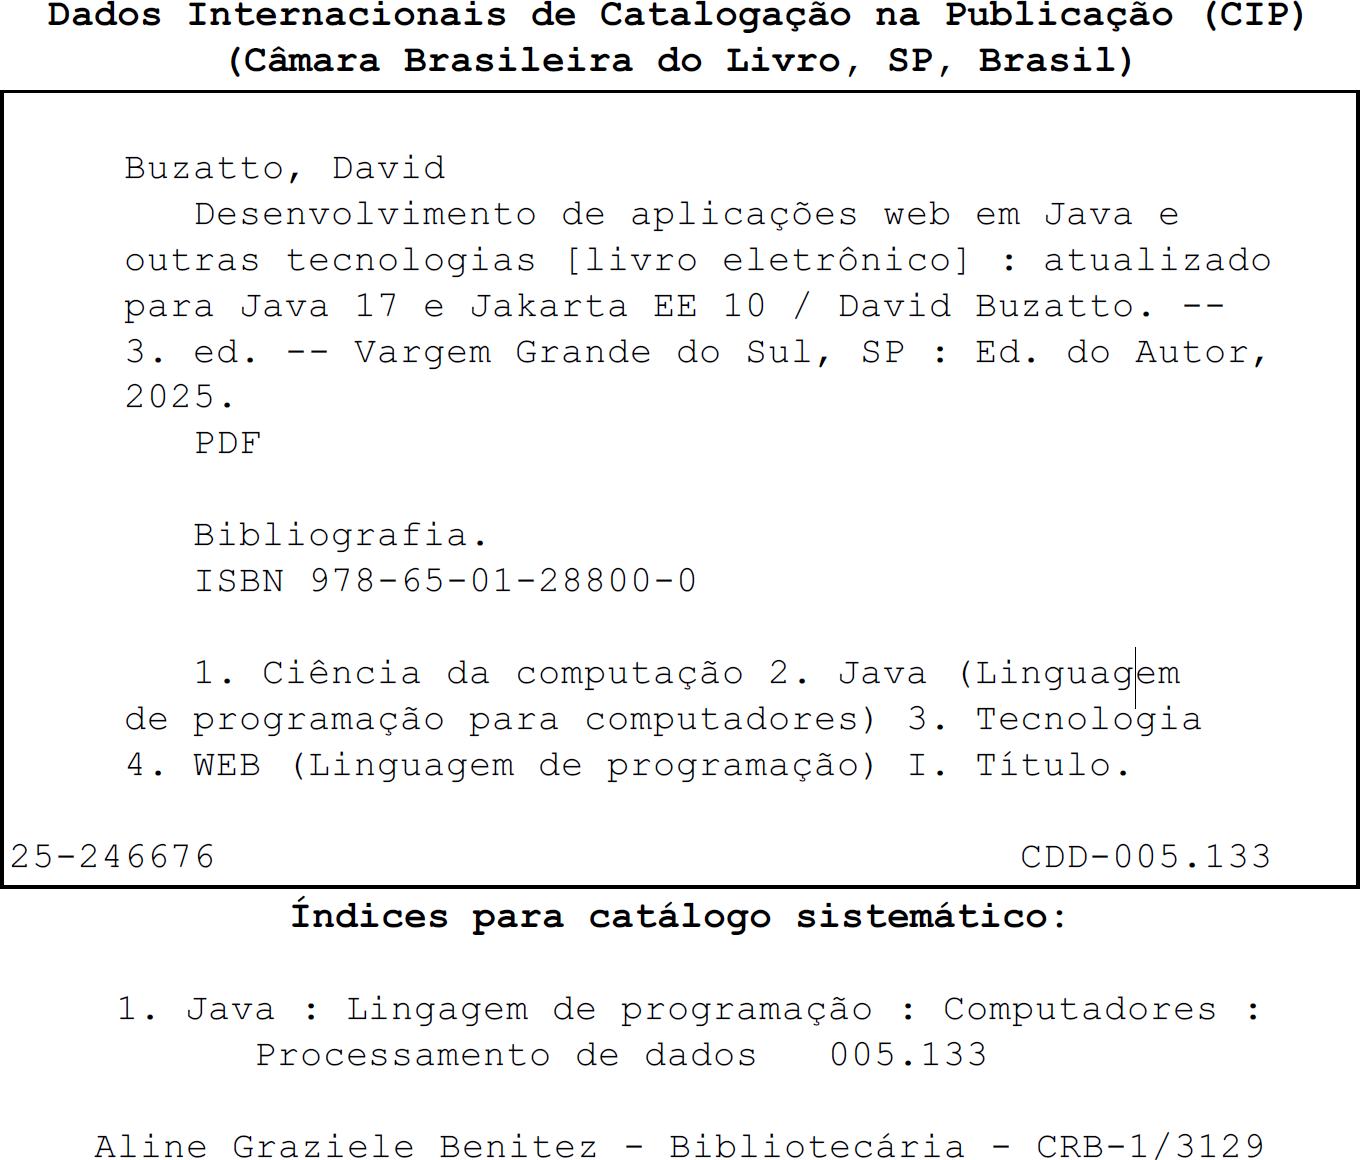
\includegraphics[scale=0.45]{imagens/ficha-978-65-01-28800-0-3ed}
    \end{figure}
    
    \restoregeometry
}

%{
%    \thispagestyle{empty}
%    \newgeometry{margin=4cm}
%    
%    \vspace*{\fill}
%    Ficha Catalográfica
%    
%    \restoregeometry
%}
%\begin{titlingpage}
    
    \thispagestyle{empty}
    \newgeometry{margin=4cm}
        
    \vspace*{\fill}
   	\centering
   	\noindent
    \noindent\rule{5cm}{0.4pt}\\
    \vspace*{0.4cm}
    \large\textit{À Aurora,\\luz da minha vida}\\
    \noindent\rule{5cm}{0.4pt}
    \vspace*{\fill}
    
    \restoregeometry
    
\end{titlingpage}

\renewcommand\chaptitlefont{\normalfont\huge\bfseries\scshape\color{corTema}}
    
%\pdfbookmark[0]{\listfigurename}{lof}
%\listoffigures*
%\cleardoublepage

%\pdfbookmark[0]{\listtablename}{lot}
%\listoftables*
%\cleardoublepage

\renewcommand\contentsname{Sumário}
\pdfbookmark[0]{\contentsname}{toc}
\tableofcontents*
\cleardoublepage

\chapter*{Prefácio}
\addcontentsline{toc}{chapter}{Prefácio}
\chaptermark{Prefácio}
\epigraph{``\textit{Any fool can write code that a computer can understand. Good programmers write code that humans can understand}''.}{Martin Fowler}

\lettrine[lines=4, lhang=0.1, lraise=0, loversize=0.2, findent=0.1em]{\textcolor{corTema}{P}}{rezado} leitor, seja bem-vindo! Os Capítulos deste livro foram organizados de forma a guiá-lo no processo de fixação dos conteúdos aprendidos durante a sua leitura por meio de exercícios, desafios e de projetos práticos aplicados no contexto de desenvolvimento de aplicações Web em Java e outras tecnologias. A ordem dos Capítulos obedece a um caminho lógico que será empregado para auxiliá-lo no processo de aprendizagem das tecnologias e técnicas discutidas, ou seja, a organização dos Capítulos segue a ordem cronológica dos tópicos que serão apresentados, ensinados e treinados.

\begin{wrapfigure}{R}{0.3\textwidth}
    \centering
    
\includegraphics[width=0.25\textwidth]{imagens/david}
\end{wrapfigure}

Antes de começar, eu gostaria de me apresentar. Meu nome é David Buzatto e sou Bacharel em Sistemas de Informação pela Fundação de Ensino Octávio Bastos (2007), Mestre em Ciência da Computação pela Universidade Federal de São Carlos (2010) e Doutor em Biotecnologia pela Universidade de Ribeirão Preto (2017). Atualmente meus principais interesses giram em torno de temas relacionados à construção de compiladores, teoria da computação, análise e projeto de algoritmos, estruturas de dados, algoritmos em bioinformática e desenvolvimento de jogos eletrônicos. Atualmente sou professor efetivo do Instituto Federal de Educação, Ciência e Tecnologia de São Paulo (IFSP), câmpus São João da Boa Vista. A melhor forma de contatar é através do e-mail \textcolor{corTema}{\href{mailto:davidbuzatto@ifsp.edu.br}{davidbuzatto@ifsp.edu.br}}.

Para que você possa aproveitar a leitura deste livro de forma plena, vale a pena entender alguns padrões que serão utilizados neste texto. As quatro caixas apresentadas abaixo serão empregadas para mostrar, a você leitor, respectivamente, boas práticas de programação, conteúdos complementares para melhorar e aprofundar seu aprendizado, observações pertinentes ao que está sendo apresentado e, por fim, itens que precisam ser tratados com cuidado ou que podem acarretar em erros comuns de programação.

\begin{boaPratica}
    Essa é uma caixa de ``Boa Prática''.
\end{boaPratica}

\begin{saibaMais}
    Essa é uma caixa de ``Saiba Mais''.
\end{saibaMais}

\begin{observacao}
    Essa é uma caixa de ``Observação''.
\end{observacao}

\begin{atencao}
    Essa é uma caixa de ``Atenção!''.
\end{atencao}

Você notará que este este livro foi escrito de forma quase coloquial, com o objetivo de conversar com você e não com o objetivo de ser um material de pesquisa. É de suma importância que você procure implementar os exemplos apresentados e que resolva cada um dos exercícios básicos de cada Capítulo, visto que a utilização de uma linguagem de programação ou tecnologia, e mais importante ainda, a obtenção de maturidade no desenvolvimento de \textit{software}, é ferramenta primordial para o seu sucesso profissional e intelectual.

Vale ressaltar que este livro e os projetos apresentados serão constantemente atualizados, sendo assim, sempre obtenha as últimas versões dos mesmos \textcolor{corTema}{\href{https://github.com/davidbuzatto/Livro-Desenvolvimento-de-Aplicacoes-Web-em-Java/releases}{aqui}}. Espero que essa obra, de distribuição totalmente gratuita, lhe seja útil!
    

\vspace*{\fill}



\mainmatter

%\part{O Básico do Básico...}
\chapter{Java para Web}\label{cap:javaParaWeb}
\epigraph{``\textit{Uma longa viagem começa com um único passo}''.}{Lao-Tsé}

\lettrine[lines=4, lhang=0.1, lraise=0, loversize=0.2, findent=0.1em]{\textcolor{corTema}{N}}{ESTE} Capítulo teremos como objetivos entender o funcionamento e a arquitetura de aplicações Web desenvolvidas em Java, entender o funcionamento dos Servlets e dos JSPs e aprender a configurar e a utilizar a \textit{Integrated Development Environment} (IDE) Apache NetBeans para o apoio ao desenvolvimento de aplicações Web em Java.


\section{Introdução}

Para que você seja capaz de construir aplicações Web, primeiramente é preciso conhecer como esse serviço é estruturado. A \textit{World Wide Web} (WWW), ou simplesmente Web, é um serviço executado em diversos computadores interligados em uma rede mundial, sendo que em alguns desses computadores são executados programas chamados de \textbf{servidores}, enquanto na maioria dos outros são executados programas chamados de \textbf{clientes}, que se comunicam com os servidores que, por sua vez, servem recursos para esses clientes. Na Figura~\ref{fig:cap01ClienteServidor} é ilustrado um recorte desta rede mundial.

\FloatBarrier
\begin{figure}[!htbp]
    \centering
    \caption{Recorte da estrutura da WWW}
    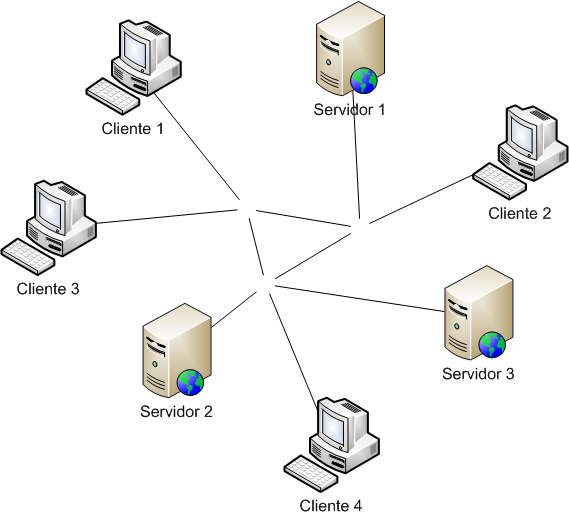
\includegraphics[scale=0.6]{imagens/cap01ClienteServidor}
    \\\textbf{Fonte:} Elaborada pelo autor
    \label{fig:cap01ClienteServidor}
\end{figure}
\FloatBarrier

Perceba que no recorte apresentado na Figura~\ref{fig:cap01ClienteServidor} são mostrados sete computadores, sendo que quatro deles atuam como clientes e os outros três como servidores. É importante entender que o que faz um computador ser cliente ou servidor é o tipo de programa que está sendo usado/executado. No nosso exemplo, as máquinas que atuam como servidores executam um programa denominado Servidor Web, que tem a capacidade de servir (disponibilizar) aos outros computadores da rede, recursos que fazem parte de uma aplicação Web, por exemplo, arquivos \textit{Hypertext Markup Language} (HTML), imagens em diversos formatos, arquivos de estilo, arquivos de \textit{script} etc. Os clientes, por sua vez, são, na maioria das vezes, os conhecidos navegadores Web, ou \textit{browsers}, que usamos no nosso dia a dia para acessar a Web e navegar em diversos \textit{sites}.

Da mesma forma que existem diversos navegadores, existem também alguns Servidores Web, sendo o Apache o mais famoso e o mais utilizado. Como já foi dito, um Servidor Web tem a função de servir recursos requisitados pelos clientes. Vamos aprender como isso funciona. Veja a Figura~\ref{fig:cap01RequestResponse}.

\FloatBarrier
\begin{figure}[!htbp]
    \centering
    \caption{Processo de requisição e resposta (\textit{request}/\textit{response})}
    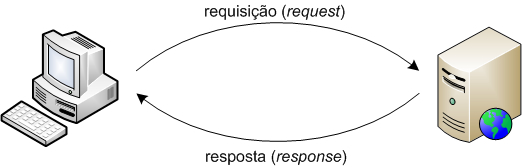
\includegraphics[scale=0.6]{imagens/cap01RequestResponse}
    \\\textbf{Fonte:} Elaborada pelo autor
    \label{fig:cap01RequestResponse}
\end{figure}
\FloatBarrier

Na Figura~\ref{fig:cap01RequestResponse} é mostrado o processo de requisição e resposta. Nesse processo, o cliente à esquerda (navegador), envia uma requisição a um recurso contido no Servidor Web (à direita) através de uma \textit{Uniform Resource Locator} (URL), sendo que nessa requisição, o cliente especifica o protocolo a ser usado, o endereço do servidor e o caminho para o recurso. Assim, uma URL tem a seguinte forma:

\begin{center}
    \textbf{\texttt{protocolo://máquina/caminho\_do\_recurso}}
\end{center}

\begin{itemize}
    
    \item Onde:
    
    \begin{itemize}
    
        \item \textbf{protocolo:} É a parte da URL que diz ao servidor qual o protocolo a ser utilizado. Quando acessamos páginas Web, por padrão, o protocolo utilizado é o \textit{Hypertext Transfer Protocol} (HTTP);
        
        \item \textbf{máquina:} É o nome ou o endereço codificado pelo \textit{Internet Protocol} (IP) da máquina que está executando o Servidor Web;
        
        \item \textbf{caminho\_do\_recurso:} É o caminho completo do recurso desejado que é disponibilizado pelo servidor.
        
    \end{itemize}
    
\end{itemize}

Confuso? Nem tanto. Vamos a um exemplo! Imagine a seguinte situação: Queremos acessar o site do IFSP. Para isso, abra o seu navegador e preencha o campo endereço com \texttt{http://www.ifsp.edu.br/} e tecle \texttt{<ENTER>}. Fazendo isso, o navegador envia uma requisição através de uma URL, usando o protocolo HTTP para a máquina \texttt{www.ifsp.edu.br}, que por sua vez retorna ao navegador uma página HTML que representa aquele endereço. 

Perceba que não especificamos o caminho do recurso! Isso não foi necessário, pois os Servidores Web são normalmente configurados para ter um comportamento padrão para responder às requisições onde só seja especificado o nome da máquina e esse comportamento padrão é direcionar para o recurso \texttt{index.html}, que é um arquivo HTML. Portanto, usar o endereço \texttt{http://www.ifsp.edu.br/} é o mesmo que usar o endereço \texttt{http://www.ifsp.edu.br/index.html}. Faça um teste! Coloque o endereço com o caminho do recurso (\texttt{index.html}) e tecle \texttt{<ENTER>}. O que aconteceu? A mesma página foi exibida não foi? Ótimo!

Vamos fazer mais um teste? Preencha novamente a barra de endereços no seu navegador com o endereço \texttt{http://j.i.uol.com.br/galerias/psp/patapon201.jpg} e tecle \texttt{<ENTER>}. Deve ter aparecido uma imagem de um jogo não foi? Vamos analisar a URL: usamos o protocolo HTTP, para pedir para o Servidor Web que está executando na máquina \texttt{j.i.uol.com.br} o recurso \texttt{patapon201.jpg}, que está armazenado no caminho \texttt{/galerias/psp/}. Este processo é ilustrado na Figura~\ref{fig:cap01ExemploRequestResponse}.

\FloatBarrier
\begin{figure}[!htbp]
    \centering
    \caption{Exemplo do processo de requisição e resposta a um recurso}
    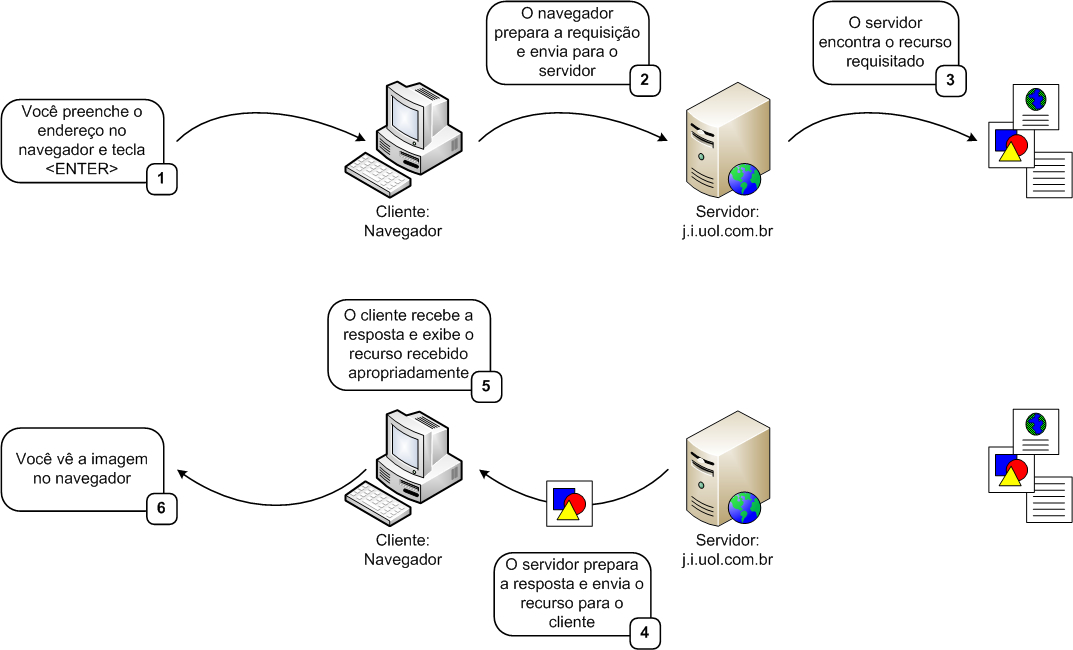
\includegraphics[scale=0.38]{imagens/cap01ExemploRequestResponse}
    \\\textbf{Fonte:} Elaborada pelo autor
    \label{fig:cap01ExemploRequestResponse}
\end{figure}
\FloatBarrier

Perceba que os passos 1, 2 e 3 da Figura~\ref{fig:cap01ExemploRequestResponse} representam o processo de requisição, enquanto os passos 4, 5 e 6 representam o processo de resposta. Note também que ao clicar em qualquer \textit{link}\footnote{O termo \textit{link} será usado para designar os \textit{hyperlinks} dos arquivos HTML} em uma página, todo esse processo é executado pelo navegador.

Muito bem! Agora que você já sabe como funciona o processo de requisição e resposta entre um navegador e um Servidor Web, podemos prosseguir com nossos estudos, agora focando em como a linguagem e a plataforma Java são utilizadas para trabalhar com aplicações Web.


\section{Contêineres de Servlets e Servidores de Aplicações}

Na Seção anterior você aprendeu algumas coisas novas\footnote{Provavelmente você já sabia disso!}, mas onde que a linguagem Java se encaixa nisso tudo? Quando criamos aplicações Web, além de termos páginas com código HTML e outros recursos como imagens, por exemplo, precisamos ter também componentes que processem informações que queremos que nossa aplicação manipule. Imagine que você vai fazer \textit{login} na sua rede social favorita (Facebook, Instagram etc.). Você preenche um campo com seu nome de usuário, sua senha e clica no botão para acessar o sistema e então eu lhe pergunto: O que acontece? Quem que vai validar seu usuário e sua senha? Como você deve saber uma página HTML não consegue fazer isso não é mesmo? Veja a tela de \textit{login} do Facebook na Figura~\ref{fig:cap01LoginFacebook}.

\FloatBarrier
\begin{figure}[!htbp]
    \centering
    \caption{Tela de login da rede social Facebook}
    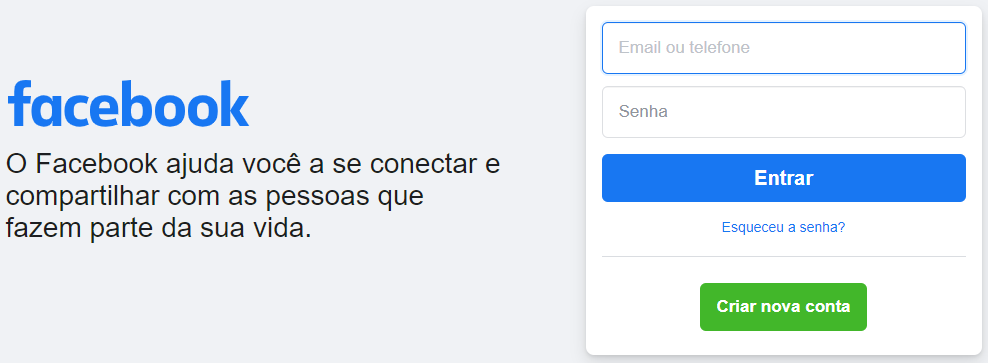
\includegraphics[scale=0.38]{imagens/cap01LoginFacebook}
    \\\textbf{Fonte:} \textit{Print screen} de \url{http://www.facebook.com}, acessado em 18/06/2021
    \label{fig:cap01LoginFacebook}
\end{figure}
\FloatBarrier

O responsável em processar os dados enviados é um componente de software que é executado no servidor em que a aplicação Web está implantada. Se a aplicação é feita em PHP, um script PHP vai fazer essa validação e retornar algum resultado com base no que foi verificado. Se a aplicação for feita em ASP.NET, Node.js etc. acontece o mesmo, ou seja, algum componente vai tratar a requisição -que enviou o usuário e a senha- e vai validá-la. Em Java é a mesma coisa!

Para que possamos utilizar código Java em nossas aplicações Web, recorremos a alguns componentes que podem ser criados dentro delas, sendo que o tipo principal desses componentes é o Servlet. Você se lembra do nosso exemplo do Facebook? Os desenvolvedores do Facebook, se usassem Java, poderiam ter criado um Servlet para receber os dados do formulário de \textit{login}, processá-los e retornar alguma resposta para o cliente, que no caso, normalmente é um navegador.

Muito bem. Sabemos então que se usarmos Java para desenvolver nossas aplicações Web, os componentes que são capazes de processar dados nas nossas aplicações e retornar resultados são os Servlets. Os Servlets são executados e gerenciados pelos Contêineres de Servlets, que funcionam como um Servidor Web simples, mas com alguns ``poderes'' a mais. Esses Contêineres também podem ser componentes de infraestruturas ainda mais robustas, que no caso são os Servidores de Aplicações. Um Servidor de Aplicações é como se fosse um Contêiner de Servlets com anabolizantes, pois além de implementar toda a especificação dos Servlets e as especificações ligadas a eles, esse tipo de servidor também implementa uma série de outras especificações da plataforma Jakarta EE (\textit{Enterprise Edition})\footnote{\url{https://jakarta.ee/}}, antigamente denominada Java EE, que fogem do propósito deste livro.

Da mesma forma que existem navegadores e Servidores Web diferentes, adivinhe só, existem também Servidores de Aplicações e Contêineres de Servlets diferentes! Iremos utilizar na nossa disciplina a implementação de referência das especificações do Jakarta EE 8, que é feita pelo Servidor de Aplicações Eclipse GlassFish 5.1.0. Trabalharemos com essa versão, que mesmo não sendo a mais recente, será a ideal para o que precisaremos fazer e que tem um melhor suporte no NetBeans. Quando estamos no mundo ``Java para Web'', várias dúvidas surgem o tempo todo, visto que existe uma infinidade de termos diferentes e que normalmente causam confusão, além de existir um ecossistema absurdamente vasto. Na próxima seção vamos aprender mais alguns detalhes teóricos e na última seção vamos realizar algumas atividades!


\section{Servlets e JSPs}

Um carro serve para dirigir. Uma televisão para assistir. Uma sandália para andar. Cada um tem suas características e vão evoluindo com o tempo. Há muito tempo atrás, quando foi inventada a televisão, a imagem que era gerada não era muito boa e era em preto e branco. Foram passando os anos e a indústria foi evoluindo o equipamento. Primeiro a imagem melhorou, depois colocaram cores, depois foram criando telas cada vez maiores, mais finas, com maior resolução, inventaram outras formas de emitir imagens, gastar menos energia elétrica e assim por diante. E daí?

Tudo evolui. O que não evolui é descartado e/ou substituído. A primeira especificação dos Servlets foi lançada em 1997 e de lá para cá, a especificação foi evoluindo, permitindo que os Servlets se tornassem componentes mais versáteis e mais fáceis de utilizar. Na versão 5.1.0 do Eclipse GlassFish (perfil \textit{Web}) que implementa as especificações do Jakarta EE 8 (perfil \textit{Web}), é implementada a especificação 4.0 dos Servlets, a especificação 2.3 das JSPs (JavaServer Pages), entre outras.

Já aprendemos que os Servlets são componentes de uma aplicação Web feita em Java e que têm a capacidade de processar dados enviados a eles e gerar respostas. Um Servlet pode gerar como resposta o código HTML de uma página, entretanto essa abordagem era utilizada nas versões mais antigas dos Servlets e é totalmente desencorajada hoje em dia. Como eu disse agora a pouco, tudo evolui. Para que os desenvolvedores não precisassem mais gerar código HTML dentro do código Java de um Servlet, foram inventadas as páginas JSP. Uma página JSP é um arquivo que pode conter –e geralmente contém– código HTML e que pode interagir diretamente com algumas funcionalidades de uma aplicação Web.

A rigor, um JSP é processado pelo Servidor de Aplicações e todo o seu conteúdo é traduzido em um Servlet, que por sua vez é compilado e executado pelo Servidor. Todo esse processo é realizado nos bastidores, então não precisamos nos preocupar com esses detalhes, mas é sempre bom saber um pouquinho como as coisas funcionam não é mesmo?

Por causa desse comportamento de tradução das JSPs para Servlets, nós podemos inserir código Java dentro das JSPs, mas novamente não iremos usar essa abordagem, muito menos irei ensinar como fazer, visto que da mesma forma que gerar HTML dentro de um Servlet manualmente é desencorajado, essa abordagem de inserir código Java dentro das JSPs também não deve ser utilizada. Uma JSP deve ser usada para exibir dados, não para processá-los diretamente usando código Java. Note que não estou dizendo que não iremos manipular dados dentro das JSPs, mas sim que existem formas seguras e corretas para fazer isso. Aprenderemos esses detalhes só no Capítulo~\ref{cap:elTagLibs}, pois até lá, já teremos aprendido outros detalhes que ainda não foram apresentados.


\section{Preparação do Ambiente de Desenvolvimento}

Nesta seção você aprenderá a instalar e configurar a IDE Apache NetBeans e o Servidor de Aplicações Eclipse GlassFish 5.1 (perfil \textit{Web}).


\subsection{Apache NetBeans}

Você conhece a linguagem Java, aprendeu a teoria e a prática da programação orientada a objetos e provavelmente usou a IDE Apache NetBeans para escrever seus códigos. Neste livro trabalharemos com a versão 12 desta IDE e nos passos abaixo é explicado como deve ser feito o \textit{download} e a instalação da mesma. Esses passos podem ser pulados caso você já tenha essa versão da ferramenta instalada em seu computador. Além disso, na playlist disponível no \textit{link} \url{https://www.youtube.com/playlist?list=PLqEuQ0dDknqVcfcBHGaYrET7IBfchVS-U} você encontrará tutoriais de preparação de ambientes de desenvolvimento para trabalhar com Java para Web, que serão mantidos atualizados.

\begin{enumerate}

    \item Acesse o endereço: \url{https://www.apache.org/dyn/closer.cgi/netbeans/netbeans/12.4/Apache-NetBeans-12.4-bin-windows-x64.exe};
    
    \item Ao acessar esse \textit{link}, a versão 12.4 do Apache NetBeans será baixada;
    
    \item Baixou? Execute o instalador. As versões atuais dos instaladores NetBeans farão a instalação completa da IDE. Basta seguir o assistente, escolher o JDK instalado (8 ou superior) e aguardar o fim da instalação.
    
\end{enumerate}

Com o NetBeans instalado, abra-o. Caso o esteja executando pela primeira vez, uma página de boas-vindas será exibida. Você pode fechá-la se quiser, além de marcar para que não seja exibida novamente. Antes de criarmos o nosso primeiro projeto Java Web, precisamos baixar, instalar e configurar o Servidor de Aplicações Eclipse GlassFish.


\subsection{Eclipse GlassFish}

Como já dito, iremos instalar a versão 5.1.0 do Eclipse GlassFish, que pode ser encontrado no \textit{link} 
\url{https://www.eclipse.org/downloads/download.php?file=/GlassFish/web-5.1.0.zip}. Como não existe um instalador, faremos a instalação manualmente. Ao terminar de baixar o arquivo, descompacte-o na sua pasta de usuário do Windows. Se fez certo, vai ter algo como \texttt{C:\textbackslash Users\textbackslash <SeuUsuário>\textbackslash glassfish5\textbackslash} no seu sistema de arquivos. Pronto! O GlassFish está instalado! A última coisa que precisaremos fazer é copiar o \textit{Driver Java Database Conectivit}y (JDBC) do Sistema Gerenciador de Banco de Dados (SGBD) MariaDB/MySQL que usaremos nos próximos Capítulos deste livro.

Para isso, baixe o arquivo acessível através do \textit{link} \url{https://downloads.mariadb.com/Connectors/java/connector-java-2.7.3/mariadb-java-client-2.7.3.jar} e, ao terminar de baixar, copie-o para o diretório \texttt{C:\textbackslash Users\textbackslash SeuUsuario\textbackslash GlassFish5\textbackslash GlassFish\textbackslash\\domains\textbackslash domain1\textbackslash lib\textbackslash}.

Por fim, vamos registrar o GlassFish no NetBeans. Com o NetBeans aberto, do lado esquerdo, clique na aba \textit{Services}. Nessa aba, há um nó chamado \destaque{\textit{Servers}}. Clique com o botão direito do mouse nele e escolha \destaque{\textit{Add Server...}}. Veja a Figura~\ref{fig:cap01Servers}.

\FloatBarrier
\begin{figure}[!htbp]
    \centering
    \caption{Registrando um servidor no NetBeans}
    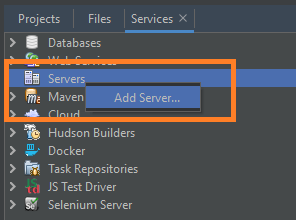
\includegraphics[scale=0.7]{imagens/cap01Servers}
    \\\textbf{Fonte:} Elaborada pelo autor
    \label{fig:cap01Servers}
\end{figure}
\FloatBarrier

Ao clicar em \destaque{\textit{Add Server...}} o assistente para registrar o servidor no NetBeans aparecerá. No primeiro passo, mostrado na Figura~\ref{fig:cap01AddServerP01}, na lista de servidores suportados, escolha \destaque{\textit{GlassFish Server}}. Na caixa de texto \destaque{\textit{Name:}} edite o nome da instância do servidor. No meu caso, adicionei a versão do mesmo, ficando ``GlassFish Server 5.1''. Ao fazer isso, clique em \destaque{\textit{Next >}}.

\FloatBarrier
\begin{figure}[!htbp]
    \centering
    \caption{Registrando um servidor no NetBeans - Passo 1}
    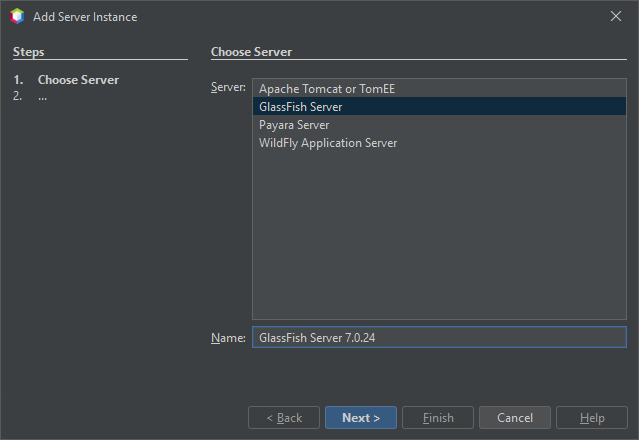
\includegraphics[scale=0.7]{imagens/cap01AddServerInstanceP01}
    \\\textbf{Fonte:} Elaborada pelo autor
    \label{fig:cap01AddServerP01}
\end{figure}
\FloatBarrier

O segundo passo do assistente precisamos definir onde os arquivos do servidor estão, como apresentado na Figura~\ref{fig:cap01AddServerP02}. Como já instalamos manualmente o servidor, não precisamos fazer o \textit{download}. Nesse passo, clique no botão \destaque{\textit{Browse...}} e procure pela instalação que fizemos há pouco. Se tudo estiver certo, a mensagem ``Detected a GlassFish...'' aparecerá logo acima dos botões dos passos do assistente. Se no seu caso estiver igual ao da Figura~\ref{fig:cap01AddServerP02}, quer dizer que está tudo certo, então basta clicar em \destaque{\textit{Next >}} para realizarmos o terceiro e último passo do assistente.

\FloatBarrier
\begin{figure}[!htbp]
    \centering
    \caption{Registrando um servidor no NetBeans - Passo 2}
    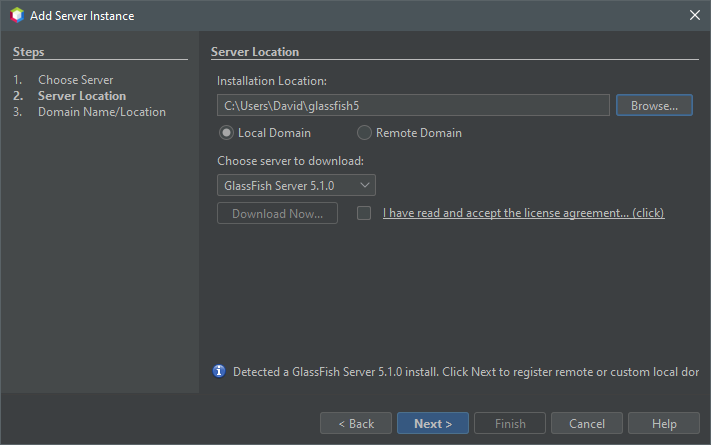
\includegraphics[scale=0.7]{imagens/cap01AddServerInstanceP02}
    \\\textbf{Fonte:} Elaborada pelo autor
    \label{fig:cap01AddServerP02}
\end{figure}
\FloatBarrier

Nesse passo, faremos a última configuração necessária, que consiste apenas em definir o nome do usuário administrador do servidor. Na Figura~\ref{fig:cap01AddServerP03} isso pode ser visto na caixa de texto \destaque{\textit{User Name:}} que está preenchida com ``admin''. Ao preencher o nome de usuário, clique em \destaque{\textit{Finish}}.

\FloatBarrier
\begin{figure}[!htbp]
    \centering
    \caption{Registrando um servidor no NetBeans - Passo 3}
    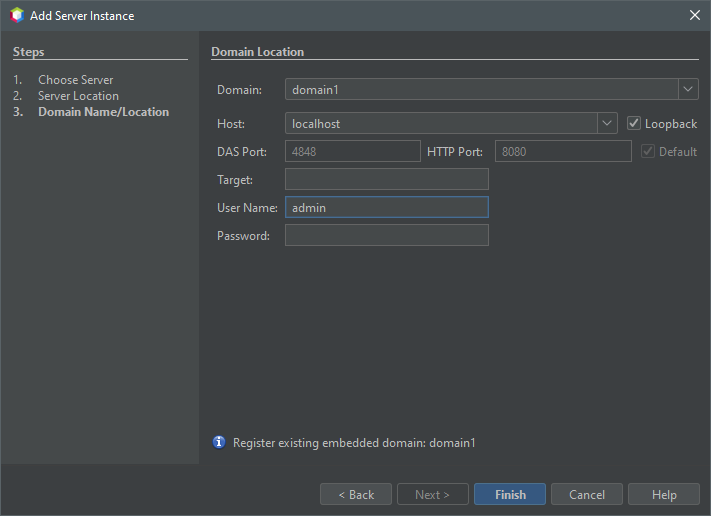
\includegraphics[scale=0.7]{imagens/cap01AddServerInstanceP03}
    \\\textbf{Fonte:} Elaborada pelo autor
    \label{fig:cap01AddServerP03}
\end{figure}
\FloatBarrier

Ao fazer isso, o GlassFish estará pronto para ser utilizado. Caso haja alguma dúvida, visite o \textit{link} mencionado que contém uma playlist de tutoriais para a configuração de ambientes de desenvolvimento.


\subsection{Primeiro Projeto Java para Web}\label{subsec:primeiroProjeto}

Agora que temos tudo configurado, iremos criar nosso primeiro projeto Java para Web! Siga os passos abaixo:

\begin{itemize}

    \item \textbf{Passo 1:} Clique no menu \destaque{\textit{File}} e depois em  \destaque{\textit{New Project...}}. Fazendo isso, o assistente para criação de projetos será aberto. Na lista de categorias, expanda o item  \destaque{\textit{Java with Ant}} e escolha  \destaque{\textit{Java Web}}. Na lista de tipos de projeto, escolha  \destaque{\textit{Web Application}} e clique no botão  \destaque{\textit{Next >}};
    
    \item \textbf{Passo 2:} Preencha o campo \destaque{\textit{Project Name:}} com ``OlaMundoWeb'' (sem acentos, sem as aspas e tudo junto). Em \destaque{\textit{Project Location:}}, defina o diretório onde o projeto será salvo. Deixe a opção \destaque{\textit{Use Dedicated Folder for Storing Libraries}} marcada e clique no botão \destaque{\textit{Next >}};
    
    \item \textbf{Passo 3:} Na opção \destaque{\textit{Server:}} escolha o ``GlassFish Server 5.1'', ou a opção com o nome que você definiu ao registrar o GlassFish. Em \destaque{\textit{Java EE Version:}} escolha ``Jakarta EE 8 Web''. Em \destaque{\textit{Context Path:}} deixe o valor padrão (/OlaMundoWeb), que é o mesmo nome que demos ao nosso projeto. Clique em \destaque{\textit{Next >}};
    
    \item \textbf{Passo 4:} No último passo, o assistente perguntará quais \textit{frameworks} nós queremos inserir no nosso projeto. Nós não vamos usar nenhum, então basta clicar em \destaque{\textit{Finish}}. Fazendo isso, o novo projeto será criado e será aberto no NetBeans, sendo que por padrão será criado um arquivo HTML (\texttt{index.html}) que será a página inicial da nossa aplicação.
    
\end{itemize}

\begin{saibaMais}
    Existem diversas definições para \textit{framework}, sendo que, informalmente, podemos definí-los como um conjunto de classes que incorporam uma abstração que tem como objetivo de solucionar problemas de um tipo ou domínio específico.
\end{saibaMais}

Muito bem, criamos nosso primeiro projeto. Vamos executá-lo para ver o que acontece? Na barra de ferramentas do NetBeans tem um botão com uma seta verde, igual a um botão de ``\textit{play}'' de um reprodutor de mídias. Quando você clicar nesse botão, você vai ver que várias mensagens começarão a aparecer na janela de saída do NetBeans. Essas mensagens irão mostrar para nós o que está acontecendo no momento, como a inicialização do GlassFish (caso não esteja iniciado) etc. O que está esperando? Clique lá no ``\textit{play}''. Assim que tudo estiver pronto, será aberta uma janela do seu navegador, onde será mostrado o conteúdo do \texttt{index.html}, que no nosso caso será uma página com ``TODO write content'' escrito.

Muito bem! Temos nossa primeira aplicação rodando no GlassFish! Fácil não é mesmo? Por enquanto não vamos nos preocupar com a estrutura do projeto, iremos aprender os detalhes aos poucos. Vamos colocar um pouco de código HTML no nosso \texttt{index.html}? Ele deve estar aberto no NetBeans. Se não estiver, procure o arquivo \texttt{index.html} na pasta \destaque{\textit{Web Pages}} do seu projeto e clique duas vezes no arquivo para abri-lo no editor. Vamos mudar o título, escrevendo ``Meu Primeiro Projeto Java para Web'' no lugar de ``TODO supply a title'' e dentro da \textit{tag} \inlineHTMLCode{<body>} do arquivo, inserir um \textit{heading} \inlineHTMLCode{<h1>} e um parágrafo com um \textit{link} para o site do IFSP. Veja na Listagem~\thechapter.\ref{listagem:projetos/capitulo01/OlaMundoWeb/web/index.html} como deve ficar seu código.

\htmlCode{Arquivo \texttt{index.html}}{projetos/capitulo01/OlaMundoWeb/web/index.html}

Salve o arquivo depois de editá-lo. Se o navegador ainda estiver aberto no \texttt{index.html}, volte a ele e aperte a tecla \texttt{<F5>} do seu teclado para mandar o navegador atualizar a página. Se não estiver, dê o ``\textit{play}'' no projeto de novo. Você vai ver que a página vai exibir as alterações que fizemos. Teste o \textit{link} para ver se está funcionando. A página deve ter ficado como mostrada na Figura~\ref{fig:cap01OlaMundoIndex}.

\FloatBarrier
\begin{figure}[!htbp]
    \centering
    \caption{Arquivo \texttt{index.html} em exibição}
    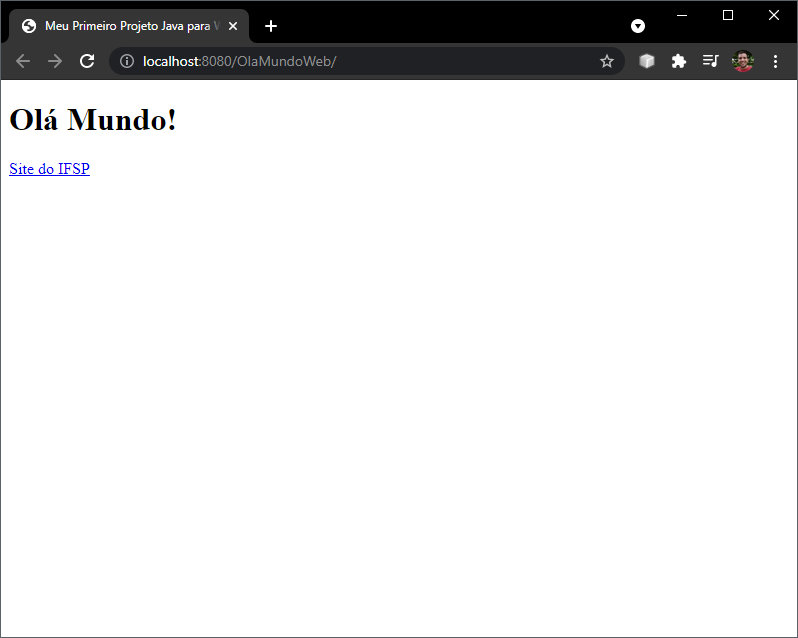
\includegraphics[scale=0.7]{imagens/cap01OlaMundoIndex}
    \\\textbf{Fonte:} Elaborada pelo autor
    \label{fig:cap01OlaMundoIndex}
\end{figure}
\FloatBarrier

Poderíamos ter usado um arquivo \textit{JavaServer Pages} (JSP) ao invés de usar um arquivo HTML, permitindo a existência de outros tipos de estruturas que vamos aprender no decorrer da disciplina, mas por enquanto vamos manter o HTML. Vamos testar os Servlets agora? Como primeiro exemplo, nós vamos criar um Servlet manualmente, enquanto os outros que vamos desenvolver durante o nosso curso serão feitos usando um assistente do NetBeans, mas essa forma fácil nós só vamos aprender a partir do Capítulo~\ref{cap:processamentoFormularios}.

Aprenderemos como criar manualmente um Servlet, para que possamos aprender alguns detalhes importantes sobre o funcionamento de aplicações Web feitas em Java. Antes disso, e daqui por diante, sempre que você criar um projeto Web, antes de qualquer coisa, siga os seguintes passos para adicionar a biblioteca necessária para viablizar o desenvolvimento.

\begin{itemize}
    
    \item \textbf{Passo 1:} Na árvore do projeto, clique com o botão direito do mouse em \destaque{\textit{Libraries}} e clique no item \destaque{\textit{Add Library...}}. Veja a Figura~\ref{fig:cap01AddLibraryProjeto};
    
    \FloatBarrier
    \begin{figure}[!htbp]
        \centering
        \caption{Inserção de bibliotecas no projeto}
        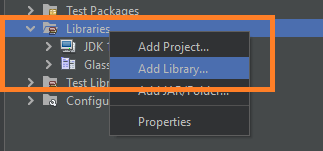
\includegraphics[scale=0.9]{imagens/cap01AddLibraryProjeto}
        \\\textbf{Fonte:} Elaborada pelo autor
        \label{fig:cap01AddLibraryProjeto}
    \end{figure}
    \FloatBarrier
    
    \item \textbf{Passo 2:} Ao fazer isso, o diálogo \destaque{\textit{Add Library}} será exibido assim como apresentado na Figura~\ref{fig:cap01AddLibraryDialog}. Clique no botão \destaque{\textit{Import...}};
    
    \FloatBarrier
    \begin{figure}[!htbp]
        \centering
        \caption{Diálogo de inserção de bibliotecas}
        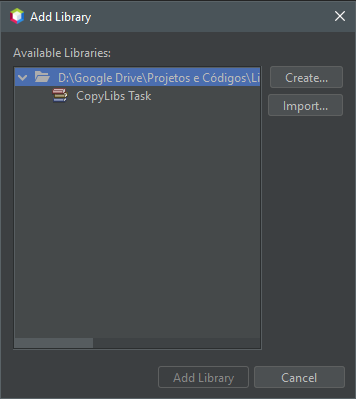
\includegraphics[scale=0.9]{imagens/cap01AddLibraryDialog}
        \\\textbf{Fonte:} Elaborada pelo autor
        \label{fig:cap01AddLibraryDialog}
    \end{figure}
    \FloatBarrier
    
    \item \textbf{Passo 3:} Outro diálogo, intitulado \destaque{\textit{Import Library}}, aparecerá. Nesse diálogo, mostrado na Figura~\ref{fig:cap01AddLibraryImport}, escolha a biblioteca \destaque{\textit{Jakarta EE Web 8 API} Library}\footnote{API é sigla para \textit{Application Programming Interface} ou Interface de Programação de Aplicações. Uma API pode ser entendida informalmente como um conjunto de funcionalidades implemetadas em uma linguagem e disponibilizadas através de interfaces públicas para que os usuários da linguagem possam usá-las.} e clique no botão \destaque{\textit{Import Library}};
    
    \FloatBarrier
    \begin{figure}[!htbp]
        \centering
        \caption{Diálogo de importação de bibliotecas}
        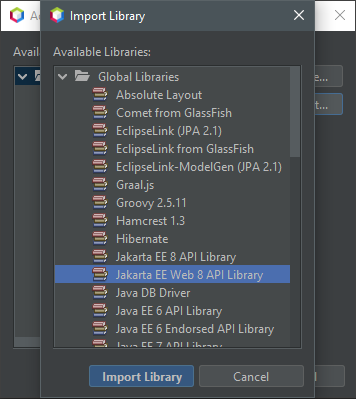
\includegraphics[scale=0.9]{imagens/cap01AddLibraryImport}
        \\\textbf{Fonte:} Elaborada pelo autor
        \label{fig:cap01AddLibraryImport}
    \end{figure}
    \FloatBarrier
    
    \item \textbf{Passo 4:} Ao fazer isso, a biblioteca será importada no projeto, ou seja, uma cópia dela será feita para dentro da sua estrutura. Note que na Figura~\ref{fig:cap01AddLibraryImported} é mostrado novamente o diálogo \destaque{\textit{Add Library}}, mas agora a biblioteca importada está disponível para ser inserida no projeto. Para isso, selecione a bibliteca e clique no botão \destaque{\textit{Add Library}};
    
    \FloatBarrier
    \begin{figure}[!htbp]
        \centering
        \caption{Diálogo de inserção de bibliotecas com biblioteca importada}
        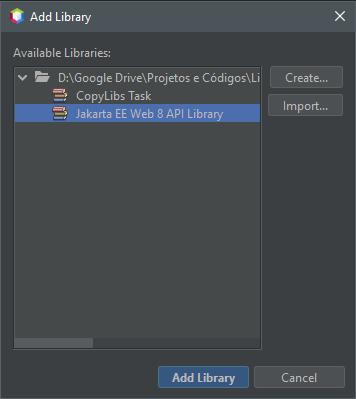
\includegraphics[scale=0.9]{imagens/cap01AddLibraryImported}
        \\\textbf{Fonte:} Elaborada pelo autor
        \label{fig:cap01AddLibraryImported}
    \end{figure}
    \FloatBarrier
    
    \item \textbf{Passo 5:} Por fim, você perceberá que a biblioteca agora faz parte das bibliotecas do projeto, podendo ser usada. Veja a Figura~\ref{fig:cap01AddLibraryFinished}.
    
    \FloatBarrier
    \begin{figure}[!htbp]
        \centering
        \caption{Biblioteca inserida no projeto}
        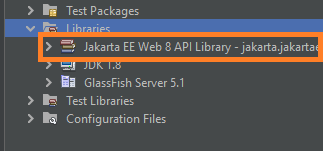
\includegraphics[scale=0.9]{imagens/cap01AddLibraryFinished}
        \\\textbf{Fonte:} Elaborada pelo autor
        \label{fig:cap01AddLibraryFinished}
    \end{figure}
    \FloatBarrier
    
\end{itemize}

Agora que importamos e inserimos a biblioteca \destaque{\textit{Jakarta EE Web 8 API Library}} no nosso projeto, podemos usar as funcionalidades Web implementadas pelo Jakarta EE. Nos próximos passos criaremos e testaremos nosso primeiro Servlet.

\begin{itemize}
    
    \item \textbf{Passo 1:} Na árvore que representa a estrutura do projeto, procure pela pasta \destaque{\textit{Source Packages}} e expanda-a (clique no sinal de ``+'' à esquerda). Dentro dela haverá um pacote com o ícone cinza chamado \destaque{\textit{<default package>}}. Como vocês devem saber, é desencorajado que se trabalhe com pacotes padrão em Java, então vamos criar um pacote. Clique com o botão direito na pasta \destaque{\textit{Source Packages}} e escolha \destaque{\textit{New}}, procure pela opção \destaque{\textit{Java Package...}} e clique nela. Se esta opção não estiver sendo exibida, clique na opção \destaque{\textit{Other...}} (no final da lista), escolha \destaque{\textit{Source Packages}} nas categorias, e \destaque{\textit{Java `Package}} nos tipos de arquivos e clique em \destaque{\textit{Next >}}. Preencha o campo \destaque{\textit{Package Name:}} com ``olamundoweb'' (sem as aspas) e clique em \destaque{\textit{Finish}}. O pacote será criado;
        
    \item \textbf{Passo 2:} Repita o Passo 1, só que agora clicando com o botão direito no pacote que você criou e crie um pacote chamado ``servlets'' (sem as aspas). O nome do pacote deverá ser preenchido com ``olamundoweb.servlets''. Seu projeto agora terá um pacote chamado ``olamundoweb.servlets''. O resultado desses dois primeiros passos podem ser vistos na Figura~\ref{fig:cap01CriacaoPacote};
    
    \FloatBarrier
    \begin{figure}[!htbp]
        \centering
        \caption{Criação do pacote \texttt{olamundoweb.servlets}}
        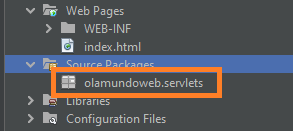
\includegraphics[scale=0.9]{imagens/cap01CriacaoPacote}
        \\\textbf{Fonte:} Elaborada pelo autor
        \label{fig:cap01CriacaoPacote}
    \end{figure}
    \FloatBarrier
            
    \item \textbf{Passo 3:} Clique com o botão direito no pacote  \destaque{\texttt{olamundoweb.servlets}}, escolha \destaque{\textit{New}} e clique na opção \destaque{\textit{Java Class...}}. Novamente, se não a encontrar, clique em \destaque{\textit{Other...}} e procure por \destaque{\textit{Java Class...}} (está na categoria ``Java'') e clique em \destaque{\textit{Next >}}. Preencha o campo \destaque{\textit{Class Name:}} com ``OlaServlet'' (sem as aspas) e clique em \destaque{\textit{Finish}}. A classe será criada dentro do pacote especificado e será aberta no editor. Você vai ter algo como apresentado na Listagem~\thechapter.\ref{listagem:projetos/capitulo01/parciais/OlaServlet.java} (sem os comentários);
    
    \javaCode{olamundoweb/servlets/OlaMundoWeb.java}{projetos/capitulo01/parciais/OlaServlet.java}
    
    \item \textbf{Passo 4:} Para que uma classe seja um Servlet, precisamos estender a classe \texttt{HttpServlet}, que está contida no pacote \texttt{javax.servlet.http}\footnote{O Jakarta EE 8 segue a nomenclatura antiga do Java EE, onde o pacote base é o \texttt{javax}. A partir da versão 9, esse pacote foi renomeado para \texttt{jakarta}.} e então implementar os métodos HTTP que queremos que nosso Servlet trate. Não se preocupe, ainda vamos aprender sobre os métodos HTTP, então o mais importante a saber, por enquanto, é que os métodos HTTP mais usados são o \texttt{GET} (\inlineJavaCode{doGet(...)} de \texttt{HttpServlet}) e o  \texttt{POST} (\inlineJavaCode{doPost(...)} de  \texttt{HttpServlet}). Então teremos que sobrescrever cada um desses métodos e ainda criaremos um terceiro que será invocado a partir dos outros dois. Confuso? Vamos ver como o código ficaria. Leia os comentários e copie o código da Listagem~\thechapter.\ref{listagem:projetos/capitulo01/OlaMundoWeb/src/java/olamundoweb/servlets/OlaServlet.java} para o seu editor.
    
\end{itemize}

\FloatBarrier
\javaCode{olamundoweb/servlets/OlaMundoWeb.java}{projetos/capitulo01/OlaMundoWeb/src/java/olamundoweb/servlets/OlaServlet.java}
\FloatBarrier
    
Até agora criamos uma classe chamada \texttt{OlaServlet}, que estende a classe \texttt{HttpServlet}. Sobrescrevemos os métodos \inlineJavaCode{doGet(...)} e \inlineJavaCode{doPost(...)} herdados de \texttt{HttpServlet} que tratam respectivamente os métodos \texttt{GET} e \texttt{POST} do protocolo HTTP e criamos um terceiro método, chamado \inlineJavaCode{processRequest(...)}, que tem a mesma assinatura dos métodos \inlineJavaCode{doGet(...)} e \inlineJavaCode{doPost(...)} e que é invocado dentro deles. É no \texttt{processRequest} que iremos colocar o código que queremos executar, sendo que no nosso exemplo, estamos mandando imprimir na saída duas Strings: ``Olá Mundo!'' e ``Meu Primeiro Servlet!''. Ou seja, se chamarmos o Servlet usando o método \texttt{GET}, o método \inlineJavaCode{doGet(...)} será invocado e passará o controle para o método \inlineJavaCode{processRequest(...)} que irá imprimir as mensagens na saída. O mesmo acontece para o método \texttt{POST}.

Muito bem, você tem um Servlet totalmente funcional, mas ai você se pergunta: ``Como vou chamar esse Servlet através do navegador?''. Então eu respondo: no código completo, você percebeu que há uma anotação chamada \inlineJavaCode{@WebServlet}? É essa anotação que vai fornecer essa informação\footnote{Antigamente precisávamos fazer o mapemanto em um arquivo \textit{Extensible Markup Language} (XML) (\url{http://pt.wikipedia.org/wiki/XML}) chamado de Descritor de Implantação (DI, em inglês \textit{Deployment Descriptor}), representado pelo arquivo \texttt{web.xml}, o que atualmente, com as versõs mais novas do Jakarta/Java EE, não é mais necessário para algumas situações.}, expecificamente no parâmetro \texttt{urlPatterns}. Perceba que configuramos esse parâmetro com um array de Strings com um elemento: ``/ola''. Com isso, podemos agora acessar o \texttt{OlaServlet} a partir de uma URL, que no nosso caso é ``\url{http://localhost:8080/OlaMundoWeb/ola}'', ou seja, usamos o protocolo HTTP, para a máquina \texttt{localhost} (que é o endereço da nossa máquina), na porta 8080 (que é a porta que o GlassFish ouve por padrão), para acessar a aplicação chamada \texttt{OlaMundoWeb} (isso vem do contexto que criamos no Passo 3 da Subseção~\ref{subsec:primeiroProjeto}, volte lá para dar uma olhadinha), para por fim acessar o recurso mapeado sob o nome de ``ola'' que no caso é o nosso Servlet. 

Sei que pode parecer um pouco confuso no começo, mas logo você vai pegar o jeito da coisa. Dê um ``play'' no projeto de novo. O navegador vai abrir no endereço da aplicação novamente. Insira o ``ola'' (sem as aspas) no final da URL e tecle \texttt{<ENTER>}. O que aconteceu? Apareceu uma página em branco não foi? É claro, afinal, nosso Servlet não gera HTML, mas apenas imprime duas mensagens na saída padrão não é mesmo? Mas como podemos ver essas mensagens? Volte no NetBeans e procure, logo abaixo, uma aba chamada \destaque{\textit{Output}}. Ela provavelmente vai estar selecionada. Dentro dela devem haver outras três abas: \destaque{\textit{OlaMundoWeb (run)}} que deve estar selecionada e que é usada para mostrar o processo de construção do projeto da nossa aplicação, \destaque{\textit{Java DB Database Process}}, que exibe o \textit{status} do Java DB e, por fim, \destaque{\textit{GlassFish Server 5.1}}, que exibe a saída padrão do GlassFish. Clique nessa última aba e veja o que está escrito lá embaixo: as duas mensagens que enviamos para a saída padrão através do método \inlineJavaCode{System.out.println(...)} dentro do Servlet, sendo que o fim de cada linha conterá os caracteres \texttt{|\#]}\footnote{Esse sufixo é inserido automaticamente pelo servidor.}! Veja o resultado na Figura~\ref{fig:cap01SaidaGlassFish}. Volte ao navegador e tecle \texttt{<ENTER>} novamente no endereço do Servlet. Volte no NetBeans. Mais duas mensagens! Fácil não é mesmo?

\FloatBarrier
\begin{figure}[!htbp]
    \centering
    \caption{Saída do GlassFish 5.1}
    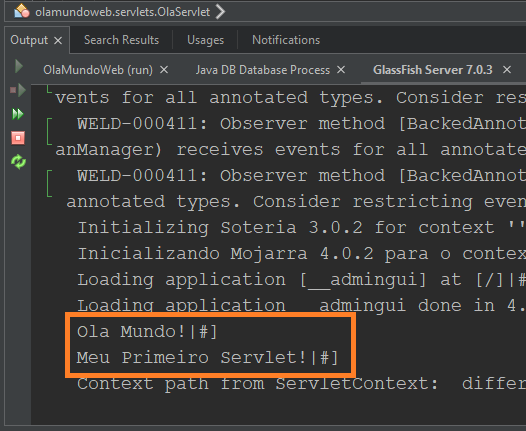
\includegraphics[scale=0.9]{imagens/cap01SaidaGlassFish}
    \\\textbf{Fonte:} Elaborada pelo autor
    \label{fig:cap01SaidaGlassFish}
\end{figure}
\FloatBarrier
    
Por mais que nosso exemplo não tenha nenhuma utilidade aparente, ele foi importante para nós entendermos o funcionamento básico de uma aplicação Web feita em Java. Nos próximos Capítulos vamos colocar o que aprendemos em prática, além de aprender várias outras coisas com o objetivo de criarmos um sistema de cadastro na forma de uma aplicação Web. Não se esqueça de praticar o que aprendemos até agora. 


\section{Resumo}

Neste Capítulo aprendemos o que é e como funciona uma aplicação Web em Java. Aprendemos a criar nosso primeiro projeto e alguns detalhes sobre a tecnologia que estamos utilizando. Executamos nossa aplicação e fizemos algumas modificações nela para vermos o que estava sendo feito. Criamos também –de forma manual– um Servlet, que como aprendemos é um dos componentes principais de uma aplicação Web em Java.


\section{Exercícios}

\begin{exercicioSemArquivo}{}{}{}
    O que é um Servidor Web?
\end{exercicioSemArquivo}

\begin{exercicioSemArquivo}{}{}{}
    Como são chamados os clientes que utilizamos para acessar aplicações servidas por um Servidor Web? Cite alguns exemplos.
\end{exercicioSemArquivo}

\begin{exercicioSemArquivo}{}{}{}
    Diferencie um Servidor Web de um Contêiner de Servlets.
\end{exercicioSemArquivo}


\section{Projetos}

\begin{projetoSemArquivo}{}{}{}
    Crie um novo projeto Java Web no NetBeans, com o nome de ``MinhaPagina'', edite o \texttt{index.html} de modo a exibir seus dados pessoais, seus interesses etc. Tente inserir uma imagem também. Dica: a imagem deve estar dentro do projeto do NetBeans. Pense se você entende o motivo pelo qual o arquivo \texttt{index.html} é mostrado por padrão quando você acessa sua página através da URL \url{HTTP://localhost:8080/MinhaPagina}.
\end{projetoSemArquivo}

\begin{projetoSemArquivo}{}{}{}
    Crie um novo projeto Java Web no NetBeans, com o nome de ``Contador''. Nesse projeto você deve criar um Servlet manualmente e dentro do método \inlineJavaCode{processRequest(...)} use uma estrutura de repetição para direcionar para a saída padrão os números de 1 a 30.
\end{projetoSemArquivo}

\begin{projetoSemArquivo}{}{}{}
    Crie um novo projeto Java Web no NetBeans, com o nome de ``Fibonacci''. Nesse projeto, você deve criar um Servlet manualmente e dentro do método \inlineJavaCode{processRequest(...)} use uma estrutura de repetição para exibir os 30 primeiros termos da série de Fibonacci. Crie um método chamado \texttt{fibonacci} dentro do seu Servlet, sendo que este método deve receber como parâmetro um inteiro e retornar um inteiro. O inteiro que é recebido como parâmetro é o número do termo desejado, enquanto o inteiro que é retornado é o termo correspondente ao parâmetro que foi recebido. A série de Fibonacci é formada inicialmente pelos números 1 e 1, sendo que os próximos números da série são gerados a partir da soma dos dois números anteriores. Os sete primeiros termos da série de Fibonacci são $1, 1, 2, 3, 5, 8, 13$, onde: $2 = 1 + 1, 3 = 1 + 2, 5 = 2 + 3, 8 = 3 + 5, 13 = 5 + 8$.
    
    Exemplos de chamadas da função fibonacci:
    \begin{itemize}
        \item \texttt{fibonacci(2)}: retorna 1
        \item \texttt{fibonacci(5)}: retorna 5
        \item \texttt{fibonacci(7)}: retorna 13
    \end{itemize}
    
\end{projetoSemArquivo}
%\chapter{Processamento de Formulários}\label{cap:processamentoFormularios}
\epigraph{``\textit{O modo como você reúne, administra e usa a informação determina se vencerá ou perderá}''.}{Bill Gates}

\lettrine[lines=4, lhang=0.1, lraise=0, loversize=0.2, findent=0.1em]{\textcolor{corTema}{N}}{ESTE} Capítulo teremos como objetivos entender o funcionamento de formulários HTML e conseguirmos diferenciar os métodos do protocolo HTTP e como tratá-los.


\section{Introdução}

Neste Capítulo vamos começar a aprender a criar algo útil! No Capítulo~\ref{cap:javaParaWeb}, aprendemos as bases do desenvolvimento Web em Java, criamos alguns programas de brinquedo\footnote{Programa de brinquedo é todo programa criado para apresentar algum conceito e que, normalmente, não tem uma utilidade prática além da pedagógica.} para aplicar as técnicas que aprendemos e agora vamos aprender mais alguns detalhes, mas dessa vez nossos programas serão mais elaborados. Vamos começar?


\section{Formulários}

A forma tradicional de se desenvolver aplicações para Web que interajam com o servidor é utilizando os chamados formulários. Um formulário é composto normalmente por um conjunto de componentes que permitem que o usuário forneça dados para serem submetidos ao servidor. Quando esses dados são recebidos pelo servidor, algum componente da aplicação vai tratá-los, sendo que no nosso caso, esse componente vai ser implementado na forma de um Servlet.

Atualmente existem diversas técnicas para a criação de aplicações Web, sendo que, dependendo da técnica/tecnologia, a forma de submeter dados ao servidor é diferente. Uma dessas técnicas é o chamado \textit{Asynchronous JavaScript and XML} (AJAX) que hoje em dia é implementado de inúmeras formas. Neste livro aprenderemos sobre AJAX no Capítulo~\ref{cap:javaScript}.

Abra o NetBeans e crie um novo projeto Java Web. Dê o nome de ``PrimeiroFormulario'' (sem as aspas). Sempre que for criar um novo projeto, siga os passos descritos na Subseção~\ref{subsec:primeiroProjeto} do Capítulo~\ref{cap:javaParaWeb}. Com o projeto criado, vamos editar o \texttt{index.html}. Nele vamos alterar o título da página e criar nosso primeiro formulário, que será usado para preenchermos dados pessoais de um cliente. Veja na Listagem~\thechapter.\ref{listagem:projetos/capitulo02/parciais/indexInicio.html} como ficou o código. Não se esqueça de copiá-lo no seu \texttt{index.html}.

\htmlCode{Protótipo do formulário de dados do cliente (\texttt{index.html})}{projetos/capitulo02/parciais/indexInicio.html}

Copiou? Salve o arquivo e execute a aplicação. Você vai ter algo como o mostrado na Figura~\ref{fig:cap02PrimeiroFormulario}.

\FloatBarrier
\begin{figure}[!htbp]
    \centering
    \caption{Visualização do protótipo do formulário de dados do cliente}
    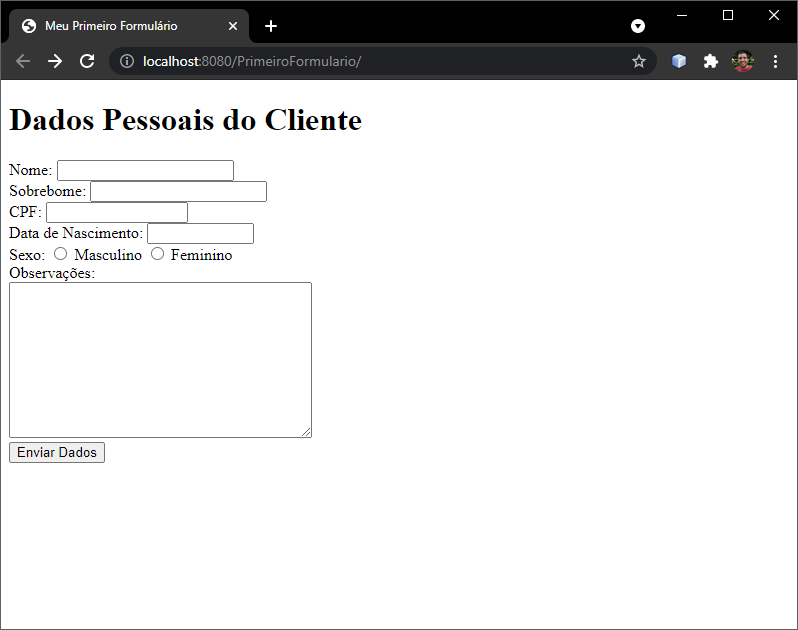
\includegraphics[scale=0.7]{imagens/cap02PrimeiroFormulario}
    \\\textbf{Fonte:} Elaborada pelo autor
    \label{fig:cap02PrimeiroFormulario}
\end{figure}
\FloatBarrier

Quanta coisa! O formulário não ficou uma obra prima, mas esse não é nosso objetivo agora. Precisamos entender o que cada \textit{tag} faz. Vamos agora analisar o código da Listagem~\thechapter.\ref{listagem:projetos/capitulo02/parciais/indexInicio.html} e entender o protótipo que fizemos. Irei detalhar apenas as \textit{tags} \inlineHTMLCode{<form>} e seus componentes, pois acredito que você já conheça as outras que foram utilizadas. Vamos lá então:

\begin{itemize}
    \item \textbf{Linha 13:} Nesta linha abrimos a \textit{tag} \inlineHTMLCode{<form>} que delimita um formulário HTML. Note que fechamos a \textit{tag} \inlineHTMLCode{<form>} na linha 43. Todas as \textit{tags} que forem inseridas entre \inlineHTMLCode{<form>} e \inlineHTMLCode{</form>} farão parte do formulário;
    
    \item \textbf{Linha 15:} Criamos um \textit{label} (tag \inlineHTMLCode{<label>}) com o conteúdo ``Nome: ''. A \textit{tag} \inlineHTMLCode{<label>} é usada para criar um rótulo. Ao invés de usar a \textit{tag} \inlineHTMLCode{<label>}, poderíamos simplesmente ter inserido o texto que queremos mostrar no formulário, mas como o texto que estamos utilizando tem o propósito de ser um rótulo para um campo do formulário, iremos utilizar essa tag para deixar nosso código mais organizado e inserir uma certa carga semântica no nosso código;
    
    \item \textbf{Linha 16:} Criamos um \textit{input} (campo de entrada) do tipo \textit{text} (texto) com tamanho de 20 colunas e com o nome de ``nome''. Dentre as \textit{tags} que representam componentes nos formulários, a \inlineHTMLCode{<input>} é uma delas. Existem vários tipos de \textit{inputs}, diferenciados pela propriedade \texttt{type}, e que vamos aprender aos poucos. A propriedade \texttt{size}, como você deve ter percebido, é utilizada para configurar a largura do campo de texto. A propriedade \texttt{name} é utilizada pelo navegador para identificar os dados do componente em questão no momento de enviar os dados para o servidor. Não entendeu a utilidade da propriedade \texttt{name}? Não se preocupe, logo vai fazer sentido;
    
    \item \textbf{Linha 17:} Usamos a \textit{tag} \inlineHTMLCode{<br/>} para pular uma linha;
    
    \item \textbf{Linhas 19 a 29:} Os próximos três campos (sobrenome, CPF e data de nascimento) são bem parecidos com o primeiro;
    
    \item \textbf{Linha 32:} Criamos um \textit{input} do tipo \textit{radio} (botão de rádio), com nome configurado como ``sexo'' e com o valor (\texttt{value}) configurado com ``M'';
    
    \item \textbf{Linha 33:} Idem à linha anterior, com a diferença que o valor é ``F''. Note que a propriedade name de ambos os radios é a mesma, pois eles representam o mesmo campo (sexo). Perceba que no navegador, se você selecionar um deles e depois clicar no outro, o que estava selecionado previamente deixa de ser selecionado. Se a propriedade \texttt{name} for diferente, eles serão considerados campos diferentes e então esse comportamento da seleção não existirá. Note ainda que você pode ``amarrar'' quantos radios você precisar;
    
    \item \textbf{Linha 38:} Nessa linha definimos uma área de texto. Esse componente, representado pela \textit{tag} \inlineHTMLCode{<textarea>} é utilizado, como o próprio nome já diz, para criar uma área de texto livre, onde o usuário poderá digitar uma quantidade arbitrária de texto. Note que para utilizar um \inlineHTMLCode{<textarea>} nós precisamos usar a \textit{tag} de fechamento (\inlineHTMLCode{</textarea>}), ao invés de fazer da forma que estamos fazendo com os \textit{inputs}. A novidade nesse componente são as propriedades \texttt{cols} e \texttt{rows}, que são usadas respectivamente para definir a quantidade de colunas e de linhas do componente;
    
    \item \textbf{Linha 41:} Por fim, nessa linha definimos um \textit{input} do tipo \textit{submit}, que é um botão que tem o comportamento padrão de, ao ser clicado, submeter (enviar) os dados do formulário para o servidor. Note que usamos a propriedade \texttt{value} para definir o texto do botão.
\end{itemize}

Agora que já conhecemos alguns dos componentes que podemos utilizar nos nossos formulários, mas você deve estar se perguntando: ``Tudo bem, o \textit{input} do tipo \textit{submit} é usado para enviar os dados do formulário para o servidor, mas onde eu digo ao \textit{submit} para onde os dados do formulário devem ser enviados?''. Vamos à resposta!

Eu tenho dito várias vezes que o componente que vai tratar os dados de um formulário na nossa aplicação é o Servlet não é mesmo? Então precisamos criar um Servlet que vai receber esses dados e então configurar o formulário para direcionar os dados inseridos nele para o Servlet apropriado.

Vamos criar o Servlet, mas agora iremos fazer de uma forma mais automática do que a que estamos fazendo desde que aprendemos a trabalhar com os Servlets. Na pasta de pacotes de código-fonte do projeto, crie um pacote chamado ``primeiroformulario.servlets'' (sem as aspas). Clique com o botão direito no pacote criado, escolha \destaque{\textit{New}} e procure pela opção \destaque{\textit{Servlet...}}. Se não encontrou, escolha a opção \destaque{\textit{Other...}}, selecione \destaque{\textit{Web}} na categoria, \destaque{\textit{Servlet}} no tipo de arquivo e clique em \destaque{\textit{Next >}}.

Preencha o campo \destaque{\textit{Class Name:}} com ``ProcessaDadosClienteServlet'' (sem as aspas) e clique em \destaque{\textit{Next >}}. Nesse passo, note que o assistente nos pede o nome do Servlet (\destaque{\textit{Servlet Name:}}) e o(s) padrão(ões) de URL (\destaque{\textit{URL Pattern(s):}}). Além disso, há a opção de inserir esses dados no descritor de implantação (\textit{deployment descriptor}), mas como estamos trabalhando com anotações para fazer o mapeamento do Servlet, essa opção deve ficar desmarcada. Falando sobre a anotação \inlineJavaCode{@WebServlet}, ao preenchermos esses campos, o NetBeans vai inserí-la para nós de forma automática! Deixe o campo \destaque{\textit{Servlet Name:}} com o valor padrão (que é o nome da classe) e preencha o campo \destaque{\textit{URL Pattern(s):}} com ``\texttt{/processaDadosCliente}'' (sem as aspas). Não iremos aprender sobre os parâmetros de inicialização (\textit{initialization parameters}) neste livro, mas nada impede que você aprenda para que eles servem, basta consultar a bibliografia recomendada nas referências bibliográficas do livro tudo bem? Tudo feito? Clique em \destaque{\textit{Finish}}.

Ao fazer isso, o nosso Servlet será criado e aberto no editor. Veja que a anotação \inlineJavaCode{@WebServlet} foi inserida apropriadamente no código da classe! Legal hein? Note também que o NetBeans já implementou o esqueleto do Servlet para nós. O primeiro método implementado é o \inlineJavaCode{processRequest(...)}. Lembra-se dele? É nele que vamos inserir o código que queremos que o Servlet execute. Após o fechamento do bloco deste método, note que existe uma linha onde está escrito ``\textit{HttpServlet methods. Click on the + sign on the left to Edit the code.}''. Siga a sugestão da frase e clique no ``+''. O que apareceu? A implementação dos métodos \texttt{GET} e \texttt{POST}, sendo que dentro delas é chamado o \inlineJavaCode{processRequest(...)}! Viu só? Da mesma forma que fazíamos manualmente! Não iremos mexer ali, então você pode contrair novamente esta seção do código clicando no sinal de ``\texttt{–}''.

Note que além de implementar o esqueleto do nosso Servlet, o NetBeans também inseriu um trecho de código dentro do \inlineJavaCode{processRequest(...)}. O código que está inserido configura o que o Servlet gerará de resposta a quem o requisitou \linebreak(\inlineJavaCode{response.setContentType(...)}), obtém o fluxo de escrita do Servlet, escreve uma série de Strings que representam uma página HTML nesse fluxo e o fecha automaticamente, dado o uso do \textit{try with resources}. Você se lembra que já falei algumas vezes que não iremos implementar Servlets que geram código HTML? Então, vamos limpar esse método, tirando todo o código que foi inserido dentro dele. Vá no editor e apague o conteúdo entre as linhas 34 (\inlineJavaCode{response.setContentType(...)}) e 46 (\texttt{\}}), incluindo elas. Seu \inlineJavaCode{processRequest(...)} deve estar vazio agora.

Antes de escrevermos nosso código, vamos a mais um pouquinho de teoria. Você se lembra, lá no comecinho do Capítulo~\ref{cap:javaParaWeb}, que eu falei que o cliente manda uma requisição para o servidor e ele manda uma resposta? Nos Servlets, essa requisição e essa resposta são representadas respectivamente por objetos do tipo \texttt{HttpServletRequest} e \texttt{HttpServletResponse}. Note que os três métodos implementados nos nossos Servlets (\inlineJavaCode{processRequest(...)}, \inlineJavaCode{doGet(...)} e \inlineJavaCode{doPost(...)}) recebem dois parâmetros, sendo eles dos tipos que mencionei. Qual a conclusão que você chega então? Os dados enviados pelo cliente ao servidor estão dentro do objeto do tipo \texttt{HttpServletRequest}, que chamamos de \texttt{request} no nosso código e os dados que enviamos de volta ao cliente, ou a quem invocou o Servlet, devem ser inseridos no objeto do tipo \texttt{HttpServletResponse}, que demos o nome de \texttt{response}.

Sabendo disso, agora ficou fácil! Os dados do formulário de clientes que estamos construindo serão recebidos pelo nosso Servlet através do objeto apontado por \texttt{request}! Legal, mas ainda falta um detalhe... Não informamos ao navegador qual o destino dos dados do formulário! Vamos fazer isso agora. Volte no \texttt{index.html} e procure pela \textit{tag} \inlineHTMLCode{<form>} (a mesma que está na linha 13 da Listagem~\thechapter.\ref{listagem:projetos/capitulo02/parciais/indexInicio.html}). Para informarmos ao navegador qual o destino do dados do formulário, utilizamos a propriedade \texttt{action}, sendo que nesta propriedade, colocamos a URL do componente que deve tratar os dados do formulário. Mapeamos nosso Servlet usando o padrão \texttt{/processaDadosCliente} não foi? Então, qual será a URL do nosso Servlet? Resposta: \texttt{processaDadosCliente}. Vamos editar nossa \textit{tag} \inlineHTMLCode{<form>} então, configurando a propriedade \texttt{action} para a URL citada. Na Listagem~\thechapter.\ref{listagem:projetos/capitulo02/parciais/indexAction.html} você pode ver como ficou o código da \textit{tag} \inlineHTMLCode{<form>}. Note que não estou listando todo o arquivo.

\htmlCode{Configurando a propriedade \texttt{action} da \textit{tag} form (\texttt{index.html})}{projetos/capitulo02/parciais/indexAction.html}

Isso quer dizer que, quando clicarmos no botão ``Enviar Dados'' (que é um \textit{input} do tipo \texttt{submit}), os dados que estiverem nos componentes que estão dentro desse formulário serão enviados para o recurso \texttt{processaDadosCliente}, que é o endereço do nosso Servlet! Já alterou o arquivo? Salvou? Legal! Atualize a página, preencha os campos e clique no botão ``Enviar Dados''. O que aconteceu? Uma página em branco foi exibida não é? E na barra de endereços, o que apareceu? O endereço do Servlet mais um monte de ``coisas''! Os detalhes sobre isso nós iremos aprender na próxima seção, então não se preocupe por enquanto.

Você se lembra dos nossos primeiros exemplos? Acessávamos o endereço do Servlet, uma página em branco era exibida e duas Strings eram direcionadas para a saída do servidor, lembra? Quem fazia esse direcionamento era o Servlet, não era? Vamos fazer a mesma coisa com o nosso Servlet de dados dos clientes, mas mostraremos os dados que foram preenchidos nos formulários. Vamos lá então?

Volte ao Servlet, vamos implementar o método \inlineJavaCode{processRequest(...)}. Qual é mesmo o nome do parâmetro do método \inlineJavaCode{processRequest(...)} que armazena os dados enviados pelo cliente? É o \texttt{request} certo? Veja o código da Listagem~\thechapter.\ref{listagem:projetos/capitulo02/PrimeiroFormulario/src/java/primeiroformulario/servlets/ProcessaDadosClienteServlet.java}. Leia todos os comentário que fiz.

\javaCode{Implementação do método \texttt{processRequest} (\texttt{ProcessaDadosClienteServlet.java})}{projetos/capitulo02/PrimeiroFormulario/src/java/primeiroformulario/servlets/ProcessaDadosClienteServlet.java}

Copiou o código? Legal. Vamos entender o que está acontecendo. Primeiramente, na linha 31, para mantermos a consistência da codificação em que os dados da nossa aplicação estão trafegando entre as camadas, configuramos o \texttt{request} para processar seus dados usando o encoding \texttt{UTF-8}. Mais adiante no livro aprenderemos a criar um filtro que fará isso automaticamente para todos os nossos Servlets, mas por enquanto vamos fazer um a um, da forma que está no código.

Na linha 41 é declarada uma variável do tipo \texttt{String} com o nome de ``nome''. Essa variável é inicializada com o valor obtido ao se chamar o método\linebreak%
\inlineJavaCode{getParameter( String param )} de \texttt{request}. O parâmetro passado ao método \inlineJavaCode{getParameter( String param )}, que é uma \texttt{String}, é o nome que foi dado ao componente do formulário, que no caso foi ``nome''. Estude as linhas 42, 43, 44, 45 e 46 e tente fazer um paralelo com o formulário contido no \texttt{index.html}. Note que a String que é passada como parâmetro no método \inlineJavaCode{getParameter(...)} sempre reflete o nome dado ao componente do formulário através da propriedade \texttt{name}. Veja a linha 44. Declaramos uma variável chamada \texttt{dataNascimento} que é inicializada com o valor do parâmetro ``dataNasc'' (configurado no formulário).

O que fizemos até a linha 46 foi criar uma variável que vai receber o valor de cada componente do formulário. A partir da linha 48, até o final do método, direcionamos para a saída os dados que foram obtidos. Vamos testar? Salve o Servlet e execute o projeto (botão de ``play'', lembra?). Na página, preencha o formulário, clique em ``Enviar Dados'' e volte no NetBeans para ver o que aconteceu. Olhe na janela de saída! Lá estão os dados que você preencheu no formulário! Muito bem! Imagine agora se esse fosse um sistema real. Esses dados recebidos dentro do Servlet poderiam alimentar uma \textit{query} SQL para inserir esse cliente em um banco de dados! Legal não é?! A partir desse ponto, você já deve estar entendendo melhor o que está acontecendo, mas e aquele monte de coisas escritas no endereço do navegador depois de clicar em ``Enviar Dados''? Esse comportamento está intrinsecamente ligado ao tipo de método HTTP que estamos usando. Vamos para a próxima Seção, vou explicar isso lá.


\section{Métodos HTTP}

O protocolo HTTP que usamos em nossas aplicações Web, define uma série de métodos que podem ser usados para tratar diversos tipos de requisições. Na nossa vida, como desenvolvedores Web, iremos nos importar com vários desses métodos. Neste Capítulo trataremos os métodos \texttt{GET} e \texttt{POST}, que são os únicos que podem ser usados em formulários HTML. Sendo assim vamos a eles.

\begin{saibaMais}
    Quer conhecer os outros métodos HTTP como \texttt{HEAD}, \texttt{PUT}, \texttt{DELETE} etc.? Acesse este link: \url{https://developer.mozilla.org/pt-BR/docs/Web/HTTP/Methods}
\end{saibaMais}


\subsection{Método GET}

O método \texttt{GET} (\textit{to get} = obter) é usado principalmente para pedir ao servidor algum recurso, sendo que ele retornará os dados requisitados, caso existam, claro. Quando nós fazemos uma pesquisa no Google ou clicamos em um \textit{link}, estamos usando o método \texttt{GET}. Qualquer URL que colocamos na barra de endereço do nosso navegador é enviada ao servidor usando o método \texttt{GET}. Vamos fazer um teste. Entre na página do Google (\url{www.google.com}) e pesquise por ``métodos http'' (sem as aspas). Ao clicar em pesquisar, o resultado será mostrado no navegador. Note que no meu caso eu fiz a busca digitando diretamente na barra do navegador Chrome. Veja a barra de endereços. Haverá algo assim:

\destaque{\texttt{https://www.google.com/search?q=métodos+http\&oq=métodos+http\&aqs=chrome.....}}

Parece grego, mas não é! Vamos entender a URL. Estamos usando o protocolo HTTP, para acessar a máquina \texttt{www.google.com} e o recurso inicia em \texttt{search} e, a partir do ponto de interrogação, são codificados os parâmetros enviados na requisição do recurso:

\destaque{\texttt{q=métodos+http\&oq=métodos+http\&aqs=chrome.....}}

Dividindo esse resto da URL nos símbolos ``\&''. Vamos obter isso aqui:

\destaque{\texttt{q=métodos+http}}\\
\destaque{\texttt{oq=métodos+http}}\\
\destaque{\texttt{aqs=chrome.....}}\\
\destaque{\texttt{...}}

Note que a forma de cada pedaço da parte correspondente aos parâmetros enviados corresponde a é \texttt{x=y}, onde ``\texttt{x}'' é o nome de um parâmetro e ``\texttt{y}'' é o valor associado a ele. No nosso exemplo, o parâmetro ``\texttt{q}'' tem o valor ``métodos+http'' que no caso é a nossa consulta! Ou seja, o componente que trata as pesquisas do Google (\texttt{search}), entenderá que o parâmetro ``\texttt{q}'' vai conter o valor da pesquisa que estamos fazendo!

Execute novamente o nosso projeto, limpe todos os campos e preencha o campo ``Nome'' com ``Juca'' (sem as aspas) e o campo ``Sexo'' com Masculino e clique em ``Enviar Dados''. Veja a URL que foi obtida na barra de endereços:

\destaque{\texttt{http://localhost:8080/PrimeiroFormulario/processaDadosCliente?}}\\
\destaque{\texttt{nome=Juca\&\\sobrenome=\&cpf=\&dataNasc=\&sexo=M\&observacoes=}}

Veja o caminho do recurso!

\destaque{\texttt{processaDadosCliente?nome=Juca\&sobrenome=\&cpf=\&dataNasc=\&}}\\
\destaque{\texttt{sexo=M\&\\observacoes=}}

O que isso quer dizer que, no nosso caso, o Servlet mapeado no endereço ``processaDadosCliente'' receberá os parâmetros \texttt{nome}, \texttt{sobrenome}, \texttt{cpf}, \texttt{dataNasc}, \texttt{sexo} e \texttt{observacoes}, receberá os valores associados a ele para serem usados e deverá, de alguma forma, retornar o recurso associado a eles. O ponto de interrogação após o mapeamento do Servlet (\texttt{/processaDadosCliente}) indica que o que vem depois dele (do ponto de interrogação) são parâmetros HTTP. Cada parâmetro, como já vimos, está na forma \texttt{x=y}, onde ``\texttt{x}'' é o parâmetro e ``\texttt{y}'' é o valor, sendo que eles são separadas por ``\&''. Então temos: \texttt{nome} igual a ``Juca'', \texttt{sobrenome} igual a vazio, \texttt{cpf} igual a vazio, \texttt{dataNasc} igual a vazio, \texttt{sexo} igual a ``M'' e \texttt{observacoes} igual a vazio. A saída no NetBeans deve ter ficado assim:

\texttt{Dados do Cliente:|\#]}\\
\texttt{Nome: Juca|\#]}\\
\texttt{Sobrenome: |\#]}\\
\texttt{CPF: |\#]}\\
\texttt{Data de Nascimento: |\#]}\\
\texttt{Sexo: Masculino|\#]}\\
\texttt{Observações: |\#]}

Vamos mandar a requisição novamente para o NetBeans, só que agora modificando a URL ao invés de usar o formulário. Dê o sobrenome de ``Santos'' ao Juca e defina o CPF como 123456789. Preencheu a URL na barra de endereços? Tecle \texttt{<ENTER>} e veja o que aconteceu no NetBeans. A saída deve ter sido essa aqui:

\texttt{Dados do Cliente:|\#]}\\
\texttt{Nome: Juca|\#]}\\
\texttt{Sobrenome: Santos|\#]}\\
\texttt{CPF: 123456789|\#]}\\
\texttt{Data de Nascimento: |\#]}\\
\texttt{Sexo: Masculino|\#]}\\
\texttt{Observações: |\#]}

Então, basicamente, ao usarmos o método \texttt{GET}, indicamos que queremos algum recurso do servidor. Quando enviamos dados através do método GET, esses dados, na forma de parâmetros, são codificados na própria URL. O nosso formulário do \texttt{index.html} utiliza por padrão o método \texttt{GET}. Qualquer formulário usa por padrão o método GET, mas se quisermos mudar o método de envio do formulário, precisamos usar a propriedade \texttt{method} da \textit{tag} \inlineHTMLCode{<form>}. Ai você me pergunta: Porque usaríamos outro método? O \texttt{GET} já não funciona? E eu respondo: Sim, o \texttt{GET} funciona, mas imagine a seguinte situação: você vai armazenar os dados de um usuário de um sistema. Você vai mandar vários dados para o servidor, inclusive uma senha. O que acontece? A senha enviada vai aparecer na URL! Afinal, a senha é um campo do formulário! O ideal seria ninguém a ver correto? Outro problema. O tamanho de uma URL é fixo! Então não podemos mandar conteúdos de tamanho arbitrário, visto que iremos perder dados caso usemos o método \texttt{GET}! Imagine mandar um vídeo para publicação no YouTube! Então como fazemos? Método \texttt{POST}, ao resgate!


\subsection{Método POST}

O método \texttt{POST} (\textit{to post} = postar) é usado para enviar qualquer tipo de dados ao servidor o que, normalmente, acarretará em algum tipo de mudança no recurso requisitado ou mesmo no servidor. Ao contrário do método \texttt{GET}, ao usar o método \texttt{POST}, os parâmetros de um formulário não são inseridos na URL, mas sim no corpo da requisição. Sendo assim, a quantidade dos dados enviados usando o método \texttt{POST} pode ter qualquer tamanho, desde apenas um parâmetro, até arquivos de tamanhos variados. Você já enviou uma foto para o Facebook não enviou? Saiba que ela foi enviada usando o método \texttt{POST}.

Como eu já disse na seção anterior, por padrão, o navegador envia os dados de um formulário usando o método \texttt{GET}. Caso queiramos mudar esse comportamento, basta usar a propriedade \texttt{method} da \textit{tag} \inlineHTMLCode{<form>}. Vamos fazer isso? Vá ao NetBeans, abra o arquivo \texttt{index.html} caso não esteja aberto, procure pela \textit{tag} \inlineHTMLCode{<form>} e insira a propriedade \texttt{method}. Veja na Listagem~\thechapter.\ref{listagem:projetos/capitulo02/parciais/indexMetodo.html} como deve ficar.

\htmlCode{Usando o método \texttt{POST} para enviar a requisição para o Servlet (\texttt{index.html})}{projetos/capitulo02/parciais/indexMetodo.html}

Salve o arquivo e execute o projeto novamente. Preencha o formulário e clique em ``Enviar Dados''. Verifique a URL, pois agora os parâmetros não serão mais codificados nela. Verifique a saída no NetBeans para constatar que os dados continuam a ser enviados. Edite novamente o \texttt{index.html} e mude o método para \texttt{GET}. Teste novamente. Os parâmetros devem estar aparecendo novamente na URL não é? De novo, edite o \texttt{index.html}, volte para o método \texttt{POST} e teste de novo.

Muito bem! Estamos quase acabando. Tenho certeza que você deve estar entendendo tudo. Se não estiver, releia o que está com dúvida tudo bem? Vamos à nossa última Seção, onde trataremos de mais um pouquinho de teoria.



\subsection{Tratando Métodos HTTP}

Você deve lembrar que quando criamos um Servlet manualmente, nós criávamos três métodos, o \inlineJavaCode{processRequest(...)}, o \inlineJavaCode{doGet(...)} e o \inlineJavaCode{doPost(...)}. Quando criamos um Servlet usando o assistente do NetBeans, ele também cria uma estrutura parecida com a que a gente criava manualmente, além de já realizar o mapeamento do nosso Servlet usando a anotação \inlineJavaCode{@WebServlet}. Na seção anterior falamos dos métodos \texttt{GET} e \texttt{POST} do protocolo HTTP, que são os que nós usamos como desenvolvedores Web. Você já deve ter notado, e eu também já falei, que um Servlet deve implementar o método HTTP que ele deve tratar. A implementação de um método HTTP em um Servlet deve ser feita dentro de métodos que por padrão são nomeados \inlineJavaCode{doXXX(...)}, onde \texttt{XXX} deve ser trocado pelo nome do método HTTP em questão. Sendo assim, requisições usando o método \texttt{GET} são tratadas dentro do método \inlineJavaCode{doGet(...)} do Servlet. Requisições usando o método \texttt{POST} são tratadas dentro do método \inlineJavaCode{doPost(...)} do Servlet e assim por diante.

Note então que todos os Servlets que criamos até agora se comportam da mesma forma tanto para o método \texttt{GET} quanto para o método \texttt{POST}, pois sempre que a requisição chega no Servlet, o método apropriado é escolhido, entretanto, tanto o método \inlineJavaCode{doGet(...)}, quanto o método \inlineJavaCode{doPost(...)}, direcionam o fluxo de execução para o método \inlineJavaCode{processRequest(...)}!
 
Muito legal não é mesmo? Com isso fechamos este Capítulo. No próximo iremos aprender a trabalhar com dois recursos importantes da especificação das JSPs: \textit{Expression Language} (EL) e TagLibs. Após aprender essas duas funcionalidades, estaremos prontos para começar a criar nosso primeiro projeto que trabalha com banco de dados, mas antes disso ainda iremos formalizar e aprender algumas coisinhas. Ah, não se esqueça de praticar o que aprendemos até agora! Vamos ao resumo do Capítulo.


\section{Resumo}

Neste Capítulo demos um passo muito importante para a nossa vida como desenvolvedores Web, pois aprendemos a trabalhar com formulários e entendemos o funcionamento dos métodos GET e POST que fazem parte do protocolo HTTP. Como você já deve ter percebido, os formulários desempenham um papel importantíssimo nas aplicações Web. Tenho certeza que de agora em diante, sempre que você usar uma aplicação Web, você saberá como aquele formulário funciona. Para colocar em prática o que aprendemos, criamos um projeto Java Web no NetBeans e fizemos diversos testes.

\section{Exercícios}

\begin{exercicioSemArquivo}{}{}{}
    Qual a diferença entre os métodos \texttt{GET} e \texttt{POST}? Quando devemos utilizar um ou o outro?
\end{exercicioSemArquivo}

\section{Projetos}

\begin{projetoSemArquivo}{}{}{}
    Incremente o projeto que criamos durante o Capítulo inserindo mais alguns campos no formulário: email, logradouro, número, complemento, cidade, estado, CEP, se o cliente tem ou não filhos. Utilize apropriadamente os tipos de \textit{input} que aprendemos até agora.
\end{projetoSemArquivo}

\begin{projetoSemArquivo}{}{}{}
    Crie um novo projeto Java Web, com o nome de ``FormularioDVD'' (sem as aspas), que deve ter um formulário usado para enviar dados de um DVD. Um DVD, no nosso caso, deve ter: número, título, ator/atriz principal, ator/atriz coadjuvante, diretor/diretora e ano de lançamento. Para tratar o formulário, crie um Servlet usando o assistente do NetBeans. Esse Servlet deve obter os dados enviados através do formulário e imprimi-los na saída padrão usando \inlineJavaCode{System.out.println(...)}, como foi feito no exemplo construído durante este Capítulo. Esse formulário deve usar o método \texttt{POST}.
\end{projetoSemArquivo}

\begin{projetoSemArquivo}{}{}{}
    Crie um novo projeto Java Web, com o nome de ``FormularioProduto'' (sem as aspas), que deve ter um formulário usado para enviar dados de um Produto. Um Produto, no nosso caso, deve ter: código de barras, descrição, unidade de medida (unidade ou kg), quantidade por embalagem, fabricante (nome). Para tratar o formulário, crie um Servlet usando o assistente do NetBeans. Esse Servlet deve obter os dados enviados através do formulário e imprimi-los na saída padrão usando \inlineJavaCode{System.out.println(...)}, como foi feito no exemplo construído durante este Capítulo. Esse formulário deve usar o método \texttt{POST}.
\end{projetoSemArquivo}

\begin{projetoSemArquivo}{}{}{}
    Crie um novo projeto Java Web, com o nome de ``CalculadoraWeb'' (sem as aspas), que deve ter um formulário usado para atuar como uma calculadora. Nesse formulário, deve haver dois campos (``número 1'' e ``número 2'') e um conjunto de radios para representar a operação a ser realizada (adição, subtração, multiplicação e divisão). Para tratar o formulário, crie um Servlet usando o assistente do NetBeans. Esse Servlet deve obter os dados enviados através do formulário, executar a operação escolhida pelo usuário e imprimir o resultado na saída padrão usando \inlineJavaCode{System.out.println(...)}, como foi feito no exemplo construído durante este Capítulo. Esse formulário deve usar o método \texttt{GET}. Faça testes de envio dos dados usando apenas a URL gerada depois da primeira submissão.
\end{projetoSemArquivo}

\begin{projetoSemArquivo}{}{}{}
    Crie um novo projeto Java Web, com o nome de ``TamanhoString'' (sem as aspas), que deve ter um formulário com apenas um campo usado para enviar uma String de qualquer tamanho para um Servlet. Utilize uma \inlineHTMLCode{<textarea>} para o usuário poder inserir essa String no formulário. O Servlet deve obter a String enviada e imprimir a quantidade de caracteres da String na saída padrão usando \inlineJavaCode{System.out.println(...)}, como foi feito no exemplo construído durante este Capítulo. Qual método HTTP deve ser utilizado nessa situação? Justifique sua resposta.
\end{projetoSemArquivo}

\begin{projetoSemArquivo}{}{}{}
    Crie um novo projeto Java Web, com o nome de ``EhPrimo'' (sem as aspas), que deve ter um formulário usado para enviar um número inteiro para um Servlet, que por sua vez deve verificar se este número é primo. O resultado do teste deve ser impresso na saída padrão. Esse formulário deve usar o método \texttt{GET}.
\end{projetoSemArquivo}

\begin{projetoSemArquivo}{}{}{}
    Crie um novo projeto Java Web, com o nome de ``EquacaoSegundoGrau'' (sem as aspas), que deve ter um formulário usado para enviar os coeficientes de uma equação de segundo grau para um Servlet, que por sua vez deve calcular as raízes da equação em questão e imprimir essas raízes na saída padrão. As raízes de uma equação do segundo grau podem ser determinadas usando a fórmula de Bhaskara \url{http://pt.wikipedia.org/wiki/Bhaskara_II}. O Servlet deve verificar também se os coeficientes passados representam uma equação do segundo grau válida. Esse formulário deve usar o método \texttt{GET}.
\end{projetoSemArquivo}
%\chapter{\textit{Expression Language} e \textit{TagLibs}}\label{cap:elTagLibs}
\epigraph{``\textit{A magia da linguagem é o mais perigoso dos encantos}''.}{Edward Bulwer-Lytton}

\lettrine[lines=4, lhang=0.1, lraise=0, loversize=0.2, findent=0.1em]{\textcolor{corTema}{N}}{ESTE} Capítulo teremos como objetivo entender a sintaxe, o propósito e como utilizar tanto a \textit{Expression Language} quanto as \textit{tags} JSP, além de aprendermos a lidar com as \textit{tags} disponibilizadas na \textit{JavaServer Pages Standard Tag Library} (JSTL).


\section{Introdução}

Neste Capítulo iremos aprender duas funcionalidades muito importantes e úteis do mundo Java Web: a \textit{Expression Language} (EL) e as TagLibs. Essas duas funcionalidades nos ajudarão na tarefa de não misturar código Java nas nossas JSPs. Você se lembra quando falei que era possível inserir código Java dentro das JSPs, não lembra? Falei também que isso não deveria ser feito, pois deixa o código difícil de ler e de manter, além de fazer com que o trabalho do Web designer (que normalmente conhece mais HTML e CSS) se torne difícil, visto que ele teria que ter um bom conhecimento em Java e em como as JSPs funcionam. Usando a EL e as TagLibs, a manipulação de dados, provenientes dos Servlets, se torna muito mais fácil, pois utiliza uma sintaxe simples e fácil de entender, ajudando no trabalho de quem não conhece muito bem o funcionamento de aplicações Web em Java. Vamos começar?


\section{\textit{Expression Language} (EL)}

A EL é um recurso da especificação das JSPs que permite utilizarmos uma sintaxe especial para obter dados que gostaríamos de mostrar nas nossas páginas, além de permitir que façamos algumas outras coisas, como por exemplo, avaliar uma expressão lógica. Como de costume, iremos utilizar um projeto para aprendermos o recurso que estamos estudando. Crie um projeto Java Web com o nome ``UsandoELeTagLibs'' (sem as aspas). Nesse projeto teremos um formulário no \texttt{index.html} que terá seus dados tratados por um Servlet, que por sua vez irá fazer algum processamento e direcionar o resultado gerado para uma página JSP, chamada \texttt{exibeDados.jsp}.

Edite o \texttt{index.html} e insira um formulário. O meu ficou como mostrado na Listagem~\thechapter.\ref{listagem:projetos/capitulo03/UsandoELeTagLibs/web/index.html}. Copie o código para o seu \texttt{index.html} e teste. 

\htmlCode{Formulário para envio de dados de um produto (\texttt{index.html})}{projetos/capitulo03/UsandoELeTagLibs/web/index.html}

Note que nesse arquivo temos algumas coisas novas. A primeira novidade é a \textit{tag} \inlineHTMLCode{<style>} na linha 10. Usamos essa \textit{tag} para criar regras de estilo para formatar/estilizar a visualização do nosso nosso documento. Tudo que usarmos de formatação como alinhamento, cor de texto etc., será definido usando estilos. Esses estilos são codificados usando as folhas de estilo \textit{Cascading Style Sheets} (CSS). A sintaxe é muito simples. As definições em CSS são chamadas de seletores. Sendo assim, a definição \inlineCSSCode{.alinharDireita} (linha 11) indica que estamos definindo um seletor que é uma classe de formatação (denotada pelo ponto (.)) que tem como nome \texttt{alinharDireita}. Todas as propriedades de formatação de um seletor são inseridas entre chaves. Note que usei a propriedade \texttt{text-align} com o valor de ``right''. Ou seja, todas as \textit{tags} que usarem a classe (atributo \texttt{class}) \inlineCSSCode{.alinharDireita} vão ser formatadas de forma a alinhar seu texto à direita.

Você já deve conhecer as tabelas do HTML não é mesmo? Note que organizei todo o formulário dentro de uma tabela e que a primeira coluna da tabela usa a classe \inlineCSSCode{.alinharDireita}, que definimos no começo do arquivo. Verifique a linha 26 para ver um exemplo. Outra modificação que fiz foi em relação à \textit{action} da \textit{tag} \inlineHTMLCode{<form>}. Note que o caminho expresso na \textit{action} é o mapeamento do Servlet que tratará a requisição, assim como estamos fazendo nos Capítulos anteriores. Esse tipo de caminho se chama ``caminho relativo'', pois o mapeamento do Servlet\footnote{\texttt{http://localhost:8088/UsandoELeTagLibs/processaDadosProduto}} está no mesmo diretório em relação ao \texttt{index.html}\footnote{\texttt{http://localhost:8088/UsandoELeTagLibs/index.html}}, sendo assim, não precisamos colocar o caminho completo, pois os dois recursos estão no mesmo diretório. Ao prosseguirmos com o conteúdo, irei ensinar uma técnica muito útil para não termos problema com os caminhos dos recursos.

A última novidade no nosso formulário é o uso da \textit{tag} \inlineHTMLCode{<select>} (linha 36) que é usada para criar uma caixa de seleção (\textit{combo box}). Veja que a propriedade \texttt{name} é definida na \textit{tag} \inlineHTMLCode{<select>} e que dentro dessa \textit{tag} existem três \textit{tags} do tipo \inlineHTMLCode{<option>} (opção). A \textit{tag} \inlineHTMLCode{<option>} é usada para criar um item da caixa de seleção. Cada \texttt{option} tem um valor associado que será enviado para o servidor com base na seleção feita. Por exemplo, se a opção ``Unidade'' for selecionada, será enviado o valor ``un'' no parâmetro ``unidade'', definido na propriedade \texttt{name} da \textit{tag} \inlineHTMLCode{<select>}.

Com o formulário pronto, vamos criar uma classe que vai representar o nosso produto. Na pasta \destaque{\textit{Source Packages}}, crie um novo pacote chamado ``entidades'' (sem as aspas). Nesse pacote, crie uma classe com o nome de ``Produto'' (sem as aspas). Nosso produto contém um código, uma descrição, uma unidade de medida e uma quantidade em estoque. Sendo assim, nossa classe também terá esses quatro campos, que devem ser implementados como membros privados. Você deve ter aprendido que quando criamos uma classe, devemos tornar seus campos privados e então criar métodos públicos para configurar e obter esses dados. Em Java, nós usamos um padrão chamado JavaBeans, que define algumas regras para se nomear os métodos que serão usados. Por exemplo, nosso produto terá um membro privado chamado \texttt{quantidade}, então teremos dois métodos públicos para acessar esse campo. O método \inlineJavaCode{setQuantidade(...)} (configure a quantidade) será usado para configurar a quantidade, enquanto o método \inlineJavaCode{getQuantidade()} (obtenha a quantidade) será usado para obter o valor da quantidade. Utilizando essa abordagem de usar métodos para obter e configurar certos campos, nós obtemos o que chamamos de propriedades de uma determinada classe, pois independente de como os métodos são implementados, os usuários da classe só enxergam os métodos públicos. Lembra-se da propriedade do encapsulamento da programação orientada a objetos? Olha ela ai! Note que usamos os prefixos \texttt{set} e \texttt{get} para nomear métodos que respectivamente alteram e obtenham uma determinada propriedade do objeto. O uso desses prefixos, entre outros detalhes, é descrito no padrão JavaBeans.

Quantos detalhes hein? Veja na Listagem~\thechapter.\ref{listagem:projetos/capitulo03/UsandoELeTagLibs/src/java/entidades/Produto.java} como ficou a implementação da classe \texttt{Produto}.

\javaCode{Implementação da classe Produto (\texttt{entidades/Produto.java})}{projetos/capitulo03/UsandoELeTagLibs/src/java/entidades/Produto.java}

Com a classe \texttt{Produto} implementada, agora podemos criar objetos do tipo \texttt{Produto} que vão conter os dados obtidos no formulário. Quem obtém e processa os dados enviados pelo formulário são os Servlets, então vamos criar um. Crie o pacote ``servlets'' -no mesmo nível do pacote ``entidades'' que já foi criado- para conter o Servlet que será criado. A classe do nosso Servlet, que deverá estar dentro do pacote recém-criado, terá o nome de ``ProcessaDadosProdutoServlet'' e deverá ser mapeada para ``/processaDadosProduto'' em \destaque{\textit{URL Pattern(s):}}. A implementação do método \texttt{processRequest} do Servlet criado pode ser vista na Listagem~\thechapter.\ref{listagem:projetos/capitulo03/UsandoELeTagLibs/src/java/servlets/ProcessaDadosProdutoServlet.java}.

\javaCode{Implementação do Servlet que cria um novo Produto (\texttt{servlets/ProcessaDadosProdutoServlet.java})}{projetos/capitulo03/UsandoELeTagLibs/src/java/servlets/ProcessaDadosProdutoServlet.java}

Vamos às novidades apresentadas nesse Servlet. Entre as linhas 29 e 32 declaramos as variáveis que vão conter o valor dos campos do formulário, sendo que só obtemos os valores da descrição e da unidade de medida, pois o método getParameter retorna Strings.

Para as variáveis inteiras, nós precisamos converter o valor retornado de ``codigo'' e ``quantidade'' para inteiro. Você já deve conhecer esse tipo de conversão não é mesmo? Entre as linhas 34 e 44 usamos dois blocos \texttt{try} para verificar se a conversão de cada valor que deve ser inteiro foi bem sucedida. Caso você não conheça essa construção da linguagem, segue então uma explicação bem rápida.

O bloco \texttt{try} (tentar) é usado na linguagem Java para englobar trechos de código que, ao serem executados, podem emitir certos tipos de ``erros''. Esses ``erros'' são chamados de exceções. O método \inlineJavaCode{parseInt(...)} da classe \texttt{Integer} pode gerar um tipo desses erros quando é passado para ele uma String que não representa um número. Exemplo: imagine que no formulário dos dados do produto, você preencheu ``um'' ao invés de ``1'' no campo código. Esse valor (``um'') vai para o Servlet e quando o método \texttt{parseInt} tenta convertê-lo para um inteiro, ele verifica que ``um'' não representa um número, então ele dá um tipo de ``grito'', que avisa quem está usando o método que alguma coisa errada aconteceu. Para ouvir esse ``grito'', precisamos usar o bloco \inlineJavaCode{try} e, logo em seguida, usar um \inlineJavaCode{catch}, que é como se fosse um tipo de ``ouvido'' que só ouve um tipo de ``grito''. O \inlineJavaCode{parseInt(...)} tentou converter ``um'', não conseguiu e então gritou: ``\texttt{NumberFormatException!!!}'' Como temos um \inlineJavaCode{catch} (``ouvido'') configurado para ouvir esse tipo de ``grito'', quando o \inlineJavaCode{parseInt(...)} ``gritar'', o \inlineJavaCode{catch} vai entender o ``grito'' e vai fazer alguma coisa, que no caso é mostrar na saída ``Erro ao converter o código.''. A mesma coisa é feita para o valor da quantidade. Resumindo –o \inlineJavaCode{try} é usado para englobar uma ou mais linhas de código que potencialmente podem lançar algum tipo de exceção, sendo que a exceção que é lançada dentro do \inlineJavaCode{try} deve ser capturada em um catch correspondente. Essa explicação é uma forma bem simples de entender o mecanismo de tratamento de exceções do Java, visto que existem muitos outros detalhes, como exceções que obrigatoriamente precisam ser tratadas ou lançadas ou não precisam ser verificadas, assim como a \texttt{NumberFormatException} no nosso caso.

Voltando ao Servlet... Na linha 48 da Listagem~\thechapter.\ref{listagem:projetos/capitulo03/UsandoELeTagLibs/src/java/servlets/ProcessaDadosProdutoServlet.java} é instanciado um novo \texttt{Produto} e este é atribuído a uma referência do tipo \texttt{Produto} chamada \texttt{prod}. Entre as linhas 49 e 52 são configuradas as propriedades do produto a partir dos dados obtidos através do formulário. Na linha 56, inserimos um atributo no \texttt{request}. Damos o nome de ``produtoObtido'' a esse atributo e configuramos seu valor como sendo o produto que criamos e configuramos entre as linhas 48 a 52. Isso quer dizer que a próxima página ou Servlet que receber a requisição a partir deste Servlet, vai receber um objeto \texttt{request} com esse atributo, ou seja, o objeto ``prod'', que é um \texttt{Produto}, vai ficar acessível a outro componente da nossa aplicação! Confuso? Já você vai entender, fique calmo.

Na linha 61 criamos um \texttt{RequestDispatcher}, que é usado para direcionar o fluxo de execução do Servlet que está sendo executado para um outro recurso. No caso, esse recurso foi definido como \texttt{exibeDados.jsp}, uma página JSP que ainda vamos criar e que vai usar o atributo ``produtoObtido'' configurado no \texttt{request} para exibir os dados do produto.

Por fim, na linha 64, o método \texttt{forward} de \texttt{disp}, que é o nosso \texttt{RequestDispatcher} para o recurso \texttt{exibeDados.jsp} é invocado, passando como parâmetro o \texttt{request} e o \texttt{response} do Servlet. Quando o método \texttt{forward} é invocado, o servidor direciona o fluxo para o recurso configurado e devolve o controle para o navegador caso o recurso deva ser exibido por ele. Uma JSP, por padrão, é usada para isso não é mesmo?

O que a página \texttt{exibeDados.jsp} vai fazer é pegar o atributo ``produtoObtido'' configurado no \texttt{request} e mostrar seus dados. Vamos criar então essa página. No NetBeans, procure pela pasta chamada \destaque{\textit{Web Pages}}. Clique com o botão direito nela, escolha \destaque{\textit{New}} e procure por \destaque{\textit{JSP...}}. Se não achar essa opção, você já deve saber como proceder não é mesmo? Preencha o campo \destaque{\textit{File Name:}} com ``exibeDados'' (sem as aspas) e clique em \destaque{\textit{Finish}}. O arquivo será criado e exibido no editor. Veja na Listagem~\thechapter.\ref{listagem:projetos/capitulo03/UsandoELeTagLibs/web/exibeDados.jsp} como ficou o código depois de ser editado.

\htmlCode{Código do arquivo  (\texttt{exibeDados.jsp})}{projetos/capitulo03/UsandoELeTagLibs/web/exibeDados.jsp}

Copiou? Salvou? Faça um teste então! Execute o projeto, preencha o formulário e clique em ``Enviar Dados''. O Servlet será invocado, processará os dados e vai redirecionar para a página \texttt{exibeDados.jsp}, que por sua vez vai mostrar os dados do produto. Legal não é? Mágica? Não! Vamos entender o que está acontecendo no código do arquivo \texttt{exibeDados.jsp}. Veja as linhas 25, 29, 33 e 37. A construção \texttt{\$\{...\}} é a EL! Usando a EL, nós podemos acessar valores que estão configurados no \texttt{request} e em outros escopos também, que vamos aprender depois. No caso, o objeto \texttt{requestScope} da EL faz referência ao objeto \texttt{request} do Servlet que é gerado a partir da JSP. Lembre-se que uma JSP é convertida em um Servlet automaticamente pelo servidor!

Usar a expressão \texttt{\$\{requestScope.produtoObtido.codigo\}} em EL quer dizer: obtenha o código do objeto configurado no atributo \texttt{produtoObtido} do \texttt{request}. Lembre-se, nós configuramos no atributo ``produtoObtido'' no \texttt{request} (linha 56 da Listagem~\thechapter.\ref{listagem:projetos/capitulo03/UsandoELeTagLibs/src/java/servlets/ProcessaDadosProdutoServlet.java}) um produto, que por sua vez tem um código (acessado pelo método \texttt{getCodigo}).

O propósito da EL é obter objetos que estão ativos nos diversos escopos da aplicação e poder obter suas propriedades, sem precisar lidar diretamente com código Java. Sei que esse foi um exemplo bem simples, mas tenho certeza que você deve ter entendido. Veja que o \texttt{codigo} usado na EL é relativo ao método \inlineJavaCode{getCodigo(...)} e não ao membro privado da classe \texttt{Produto} chamado \texttt{codigo}. Essa mágica se dá pelo uso do padrão JavaBeans! Como exercício mental, analise as linhas 29, 33 e 37 e tente imaginar o que está acontecendo. Agora que já sabemos o que é a EL e como utilizá-la, vamos às \textit{tags} JSP.


\section{Tags JSP}

Na especificação das JSPs, existem uma série de \textit{tags} especiais que devem ser implementadas por quem implementa a especificação. Essas \textit{tags} são nomeadas usando o prefixo ``jsp''. Na verdade, nós quase não iremos utilizar essas \textit{tags} e as que utilizarmos, explicarei no momento oportuno, mas para você ter uma ideia de como elas funcionam, crie uma página JSP chamada ``testesTags'' na pasta \destaque{\textit{Web Pages}} do projeto que estamos trabalhando. Veja na Listagem~\thechapter.\ref{listagem:projetos/capitulo03/UsandoELeTagLibs/web/testesTags.jsp} o código que você deve copiar para o arquivo \texttt{testesTags.jsp}. 

\htmlCode{Exemplo das \textit{tags} \texttt{<jsp:useBean>} \texttt{<jsp:setProperty>}  (\texttt{testesTags.jsp})}{projetos/capitulo03/UsandoELeTagLibs/web/testesTags.jsp}

Copie o código no seu arquivo, salve e acesse o endereço \linebreak \texttt{http://localhost:8080/UsandoELeTagLibs/testesTags.jsp} no seu navegador para testar a página. O que aconteceu? O produto criado foi exibido assim ``4, Arroz, kg, 100'' não foi? Vamos analisar o código no arquivo \texttt{testesTags.jsp}. Entre as linhas 13 e 16 definimos um comentário, que nas JSPs é delimitado entre \texttt{<\%--} e \texttt{--\%>}. Esse comentário não pode ser visto no código-fonte da página HTML gerada! Nas linhas 17 e 19 usamos a \textit{tag} \inlineHTMLCode{<jsp:useBean>} para criar um objeto com nome de ``meuProduto'', configurado pelo atributo \texttt{id}, do tipo \texttt{entidades.Produto}, configurado pelo atributo \texttt{class}, que vai existir no escopo da página, ou seja, esse objeto só existe nesta página. Note que precisamos colocar o caminho completo da classe no atributo \texttt{class} para informarmos qual o tipo de objetos que queremos instanciar. A partir da linha 20, usamos a \textit{tag} \inlineHTMLCode{<jsp:setProperty>} para configurar as propriedades do objeto chamado ``meuProduto'' que foi criado usando a \textit{tag} \inlineHTMLCode{<jsp:useBean>}. Entre as linhas 20 e 22, referenciamos o objeto ``meuProduto'' e configuramos a propriedade ``codigo'' ((\texttt{property="codigo"}) com o valor ``4''. A instrução em Java equivalente a estas duas linhas é \inlineJavaCode{meuProduto.setCodigo( 4 )}. A partir da linha 33, mostramos então os dados do objeto ``meuProduto'' que foi criado usando EL. Note que desta vez, usamos \texttt{pageScope} ao invés de \texttt{requestScope}, visto que o objeto existe apenas no escopo da página (veja na linha 19).

Da mesma forma que existem as \textit{tags} JSP padrão, você pode criar suas próprias \textit{tags} que podem ter comportamentos dos mais variados possíveis, entretanto nós não iremos aprender a fazer isso. Como é possível criar \textit{tags} personalizadas, nós podemos usar conjuntos de \textit{tags} que são implementadas por terceiros em nossos projetos. Um desses conjuntos é a \textit{JavaServer Pages Standard Tag Library} (JSTL), que vamos aprender na próxima Seção. Vamos lá então!



\section{\textit{JavaServer Pages Standard Tag Library} - JSTL}

A JSTL é uma biblioteca formada por um conjunto de \textit{tags} (TagLib = \textit{tag} \textit{Library} = Biblioteca de \textit{tags}) que visam apoiar o desenvolvedor na tarefa de construir suas páginas JSP, permitindo que várias coisas possam ser feitas sem o uso direto de código Java, por exemplo, iterar por uma lista de objetos, executar testes lógicos, formatar dados, entre muitos outros. Quando formos implementar nosso primeiro projeto no Capítulo~\ref{cap:primeiroProjeto}, iremos utilizar muitos recursos da JSTL, mas por agora vamos aprender apenas como inseri-la no nosso projeto e fazer um pequeno exemplo.

Vamos implementar um exemplo bem simples. Iremos criar um \inlineJavaCode{for} usando \textit{tags} da JSTL. Crie mais uma página JSP, com o nome de ``testesJSTL''. O NetBeans vai abrir o arquivo quando este for criado. Vamos editá-lo? Copie então o código da Listagem~\thechapter.\ref{listagem:projetos/capitulo03/UsandoELeTagLibs/web/testesJSTL.jsp}.

\htmlCode{Exemplo de uso da JSTL  (\texttt{testesJSTL.jsp})}{projetos/capitulo03/UsandoELeTagLibs/web/testesJSTL.jsp}

Copiou? Testou? Se tudo deu certo, você deve ter visto uma tabela zebrada (cor sim/cor não). Veja a Figura~\ref{fig:cap03VisualizacaoTestesJSTL}.

\FloatBarrier
\begin{figure}[!htbp]
    \centering
    \caption{Visualização da página \texttt{testesJSTL.jsp}}
    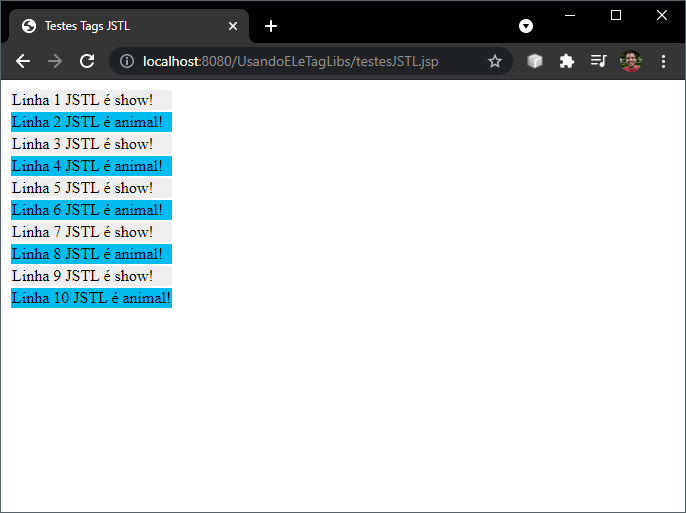
\includegraphics[scale=0.7]{imagens/cap03VisualizacaoTestesJSTL}
    \\\textbf{Fonte:} Elaborada pelo autor
    \label{fig:cap03VisualizacaoTestesJSTL}
\end{figure}
\FloatBarrier

Vamos analisar o código da Listagem~\thechapter.\ref{listagem:projetos/capitulo03/UsandoELeTagLibs/web/testesJSTL.jsp}. Talvez você tenha se assustado, mas não se preocupe, estou aqui para te explicar. Vamos começar pela primeira linha. Nessa linha, como em todos os JSPs que criamos até agora, usamos a diretiva \texttt{page}. As diretivas nos JSPs são delimitadas por \texttt{<\%@} e \texttt{\%>} e são usadas para realizar algumas configurações no Servlet que será gerado a partir do JSPs. A diretiva \texttt{page}, no nosso caso, é usada para configurar o \texttt{response} do Servlet, informando que ele vai conter um documento do tipo ``text/html'' (atributo \texttt{contentType}) e que o encoding utilizado (como os caracteres são codificados) é o UTF-8 (atributo \texttt{pageEncoding}). Veja que isso é análogo ao que estamos fazendo manualmente na primeira linha do método \inlineJavaCode{processRequest(...)} dos nossos Servlets.

Na linha 2 utilizamos a diretiva \texttt{taglib}. Essa diretiva vai permitir que nós digamos qual TagLib queremos utilizar. O atributo \texttt{uri} é usado para informarmos qual biblioteca de \textit{tags} queremos utilizar. No nosso caso, queremos utilizar as funcionalidades principais da JSTL, que são chamadas de ``core''. A \textit{Uniform Resource Identifier} (URI) para definir isso é a \texttt{http://java.sun.com/jsp/jstl/core}. O outro atributo, \texttt{prefix} (prefixo), nos permite definir um prefixo para usar as \textit{tags}. O prefixo padrão para a parte ``core'' da JSTL é ``c'', mas podemos usar o prefixo que quisermos. Para manter o padrão, iremos usar o ``c'' mesmo. Assim, quando qualquer desenvolvedor Web que conheça a JSTL bater o olho no código e ver alguma \textit{tag} que inicie com ``\texttt{c:}'' vai saber que a \textit{tag} que está sendo utilizada faz parte do core da JSTL.

Entre as linhas 12 e 20 definimos duas classes CSS. Sendo que uma usaremos para colorir o fundo das linhas pares de uma tabela, enquanto a outra será usada para colorir o fundo das linhas ímpares. A propriedade usada em ambas as classes é a \texttt{background} (fundo), sendo que em cada uma usamos uma cor diferente usando a notação \textit{Red Green Blue} (RGB) em hexadecimal. Nas linhas 25 e 40 delimitamos uma tabela.

\begin{saibaMais}
    Nunca ouviu falar de cores na notação em hexadecimal? De uma olhada nesses links: \url{http://dematte.at/colorPicker/}, \url{http://paletton.com/}, \url{https://pt.wikipedia.org/wiki/Tripleto_hexadecimal} e \url{http://en.wikipedia.org/wiki/Web_colors}
\end{saibaMais}

Na linha 26, usamos a \textit{tag} \inlineHTMLCode{<c:forEach>} (olhe o prefixo!), usada para iterar um determinado número de vezes ou sobre alguma lista de objetos. No nosso caso, queremos que o que está entre \inlineHTMLCode{<c:forEach>} e \inlineHTMLCode{</c:forEach>} seja executado dez vezes, pois definimos que a iteração deve iniciar em 1, usando o atributo \texttt{begin}, e ir até 10, usando o atributo \texttt{end}. Queremos também que o \textit{status} da iteração seja armazenado na variável \texttt{i}, definida no atributo \texttt{varStatus}. Então temos um \inlineJavaCode{for} que vai executar dez vezes. Durante estas dez iterações, vamos construir nossa tabela, inserindo linhas nela com apenas uma coluna, mas queremos que as linhas pares sejam coloridas usando a classe \inlineCSSCode{.linhaPar}, enquanto que as linhas ímpares sejam coloridas usando a classe \inlineCSSCode{.linhaImpar}. Sabemos que todo número par tem resto igual à zero numa divisão por dois, correto? Então precisamos saber em qual iteração estamos, calcular o resto e verificar se é zero. Se for, cria uma linha da tabela usando a classe \inlineCSSCode{.linhaPar}, caso contrário, usa \inlineCSSCode{.linhaImpar}.

Para criar séries de testes lógicos como numa estrutura \texttt{if/else}, nós usamos a \textit{tag} \inlineHTMLCode{<c:choose>} (\textit{to choose} = escolher) e dentro dela colocamos as condições que queremos testar usando a \textit{tag} \inlineHTMLCode{<c:when>} que é equivalente aos \texttt{if’s} e \texttt{else if’s} e, por fim, se necessário, usamos a \textit{tag} \inlineHTMLCode{<c:otherwise>} que é equivalente ao \inlineJavaCode{else}. Vamos analisar o código então: entre as linhas 27 e 38 nós definimos nossa estrutura condicional usando a \textit{tag} \inlineHTMLCode{<c:choose>}. Dentro dela, definimos na linha 28 uma \textit{tag} \inlineHTMLCode{<c:when>}, que testa (atributo \texttt{test}) se a divisão da propriedade \texttt{count} da variável \texttt{i} por dois é igual a zero (par). Note o uso da EL e que podemos executar operações aritméticas dentro dela! Se o resultado for \inlineJavaCode{true}, o número é par e o conteúdo deste \inlineHTMLCode{<c:when>} é gerado, ou seja, uma linha da tabela usando a classe \inlineCSSCode{.linhaPar}. Caso contrário, como não temos mais nenhum \inlineHTMLCode{<c:when>}, é gerado o código dentro do \inlineHTMLCode{<c:otherwise>}, que por sua vez também gera uma linha da tabela, só que usando a classe \inlineCSSCode{.linhaImpar}. Fique à vontade para mudar o conteúdo gerado dentro de cada linha, bem como as classes.

Viu como não é tão complicado? Na verdade é bem simples e fácil de usar, mas precisamos praticar para ficarmos craques. Depois dessa introdução à EL e a JSTL, nós já estamos quase prontos para começarmos o nosso primeiro projeto Web de verdade, mas ainda temos que formalizar algumas coisas que serão vistas no próximo Capítulo~\ref{cap:padroesDeProjeto}. Novamente, não se esqueça de praticar o que fizemos até agora.  


\section{Resumo}

Neste Capítulo nós aprendemos a criar um formulário que teve seus dados tratados por um Servlet, que por sua vez redirecionou o fluxo da aplicação para outra página JSP, utilizada para mostrar os dados informados no formulário. Com isso, tivemos uma noção do que é a EL e como ela funciona. Depois aprendemos um pouco sobre as \textit{tags} padrão da especificação dos JSPs e, por fim, aprendemos utilizar a JSTL em nosso projeto, além de fazermos alguns testes. No Capítulo~\ref{cap:padroesDeProjeto} vamos dar uma paradinha com os JSPs e Servlets para podermos aprender como estruturar um projeto Web que trabalha com banco de dados. Tenho certeza que você vai gostar bastante.


\section{Exercícios}

\begin{exercicioSemArquivo}{}{}{}
    Explique, com suas palavras, qual a importância da EL.
\end{exercicioSemArquivo}

\begin{exercicioSemArquivo}{}{}{}
    Justifique porque é melhor usar a JSTL ou qualquer outra TagLib ao invés de usar código Java diretamente nas JSPs.
\end{exercicioSemArquivo}

\section{Projetos}

\begin{projetoSemArquivo}{}{}{}
    Modifique o Projeto~\ref{cap:processamentoFormularios}.1 do Capítulo~\ref{cap:processamentoFormularios} para executar da mesma forma que o projeto criado neste Capítulo, ou seja, o formulário deve submeter os dados para um Servlet, que por sua vez deve criar e enviar um objeto através do \texttt{request} para um JSP, que deve exibir ao usuário usando EL.
\end{projetoSemArquivo}

\begin{projetoSemArquivo}{}{}{}
    Modifique o Projeto~\ref{cap:processamentoFormularios}.2 do Capítulo~\ref{cap:processamentoFormularios} para executar da mesma forma que o projeto criado neste Capítulo, ou seja, o formulário deve submeter os dados para um Servlet, que por sua vez deve criar e enviar um objeto através do \texttt{request} para um JSP, que deve exibir ao usuário usando EL.
\end{projetoSemArquivo}

\begin{projetoSemArquivo}{}{}{}
    Você já sabe que uma JSP na verdade é um Servlet não é mesmo? Será então que podemos definir na \texttt{action} de um formulário o endereço de um arquivo JSP ao invés de um Servlet? Crie um novo projeto Java Web, chamado ``JSPTrataFormulario'', onde você deve ter um formulário no \texttt{index.html} que contenha dois campos: nome e idade. A action deste formulário deve apontar para um arquivo JSP chamado ``exibeDadosForm.jsp'' (sem as aspas). Nesse arquivo, você deve mostrar os dados recebidos do formulário do \texttt{index.html} usando EL. Dica: para acessar os parâmetros do \texttt{request} usando EL, usa-se \texttt{\$\{param.nomeDoParametro\}}. Por exemplo, o parâmetro idade é acessado usando \texttt{\$\{param.idade\}}.
\end{projetoSemArquivo}

\begin{projetoSemArquivo}{}{}{}
    Crie um novo projeto Java Web, com o nome de ``TabelaArbitraria'', onde no \texttt{index.html} você deve ter um formulário que pede ao usuário que seja digita a quantidade de linhas e de colunas que ele deseja que uma tabela seja gerada. Aponte a \texttt{action} deste formulário para outro arquivo JSP, chamado ``montadorTabela.jsp'', que obtém os dados enviados pelo formulário do \texttt{index.html} usando EL e usa dois \inlineHTMLCode{<c:forEach>} aninhados para construir a tabela de dimensões arbitrárias. Monte a tabela somente se o tamanho de linhas e de colunas for maior que zero. Se não for, exiba uma mensagem ao usuário. Dica: para testar se duas condições são verdadeiras, ou seja, se \texttt{param.colunas > 0} e \texttt{param.linhas > 0}, use o operador \texttt{and} (e) da EL, enquanto o operador ``maior que'' é o \texttt{gt} (\textit{greater than}). Ou seja, \texttt{test="\$\{(param.linhas gt 0) and (param.colunas gt 0)\}"}.
\end{projetoSemArquivo}
%\chapter{Padrões de Projeto: \textit{Factory}, DAO e MVC}\label{cap:padroesDeProjeto}
\epigraph{``\textit{É longo o caminho que vai do projeto à coisa}''.}{Molière}

\lettrine[lines=4, lhang=0.1, lraise=0, loversize=0.2, findent=0.1em]{\textcolor{corTema}{N}}{ESTE} Capítulo teremos como objetivo entender e aplicar os Padrões de Projeto \textit{Factory}, DAO e MVC. Além disso iremos aprender a integrar o acesso à banco de dados em uma aplicação Java.


\section{Introdução}

A partir de agora iremos dar um passo importantíssimo em nossos estudos sobre desenvolvimento de software, pois iremos aprender a lidar com um banco de dados em um sistema de testes que iremos construir. Isso nos dará o embasamento necessário para que no Capítulo~\ref{cap:sistemaControleClientes} nós consigamos fazer essa mesma integração em aplicações Web. Além de aprendermos a conectar nossa aplicação com uma base de dados, iremos aprender também alguns padrões de projeto que nos ajudarão a organizar nossa aplicação de forma a melhorar sua manutenção. 

Antes de começarmos a discussão e a implementação desses padrões, nós precisamos preparar nosso ambiente de desenvolvimento. O NetBeans já temos instalado. O Sistema Gerenciador de Banco de Dados (SGBD) que iremos utilizar, o MariaDB\footnote{Provavelmente você deve ter instalado na sua máquina o MariaDB que é distribuído junto ao XAMPP}/MySQL, você provavelmente já deve ter instalado também. Com isso pronto, precisamos instalar uma ferramenta para nos ajudar a criar nossa base de dados. Iremos utilizar o MySQL Workbench, uma ferramenta gratuita para gerenciamento do MariaDB/MySQL. 


\section{Preparando o Ambiente}\label{sec:preparandoAmbiente}

Para começar, vamos fazer o download da ferramenta. Acesse o endereço \url{https://dev.mysql.com/downloads/workbench/}, escolha Microsoft Windows como plataforma, que provavelmente é o sistema operacional que você está utilizando e clique no botão ``\textit{Download}''. Fazendo isso, você será direcionado para uma página onde é requisitado um nome de usuário e senha. Se você não quiser se cadastrar (não precisa), clique no link embaixo do formulário de \textit{login} onde está escrito ``\textit{No thanks, just start my download}''. O download do instalador será iniciado.

Baixou? Legal! Execute o instalador. Na época da elaboração desse livro, a última versão disponível era a \texttt{8.0.25}. Basta seguir os passos, fazendo a instalação completa. Ao terminar, deixe marcada a opção \destaque{\textit{Launch MySQL Workbench now}} e clique em \destaque{\textit{Finish}}. Aguarde o MySQL Workbench abrir. A interface principal da versão 8.0.25 do Workbench pode ser vista na Figura~\ref{fig:cap04MySQLWorkbench}.

\FloatBarrier
\begin{figure}[!htbp]
    \centering
    \caption{Interface principal do MySQL Workbench}
    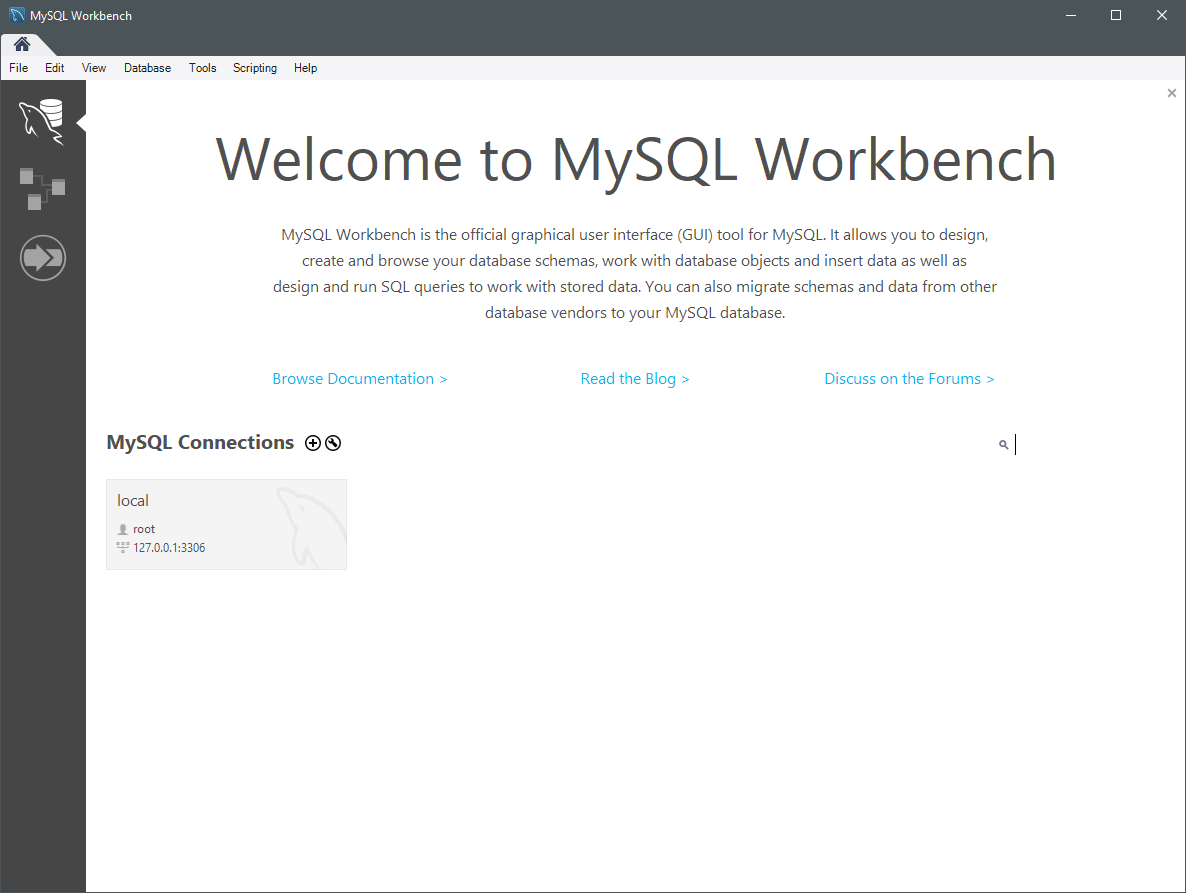
\includegraphics[scale=0.45]{imagens/cap04MySQLWorkbench}
    \\\textbf{Fonte:} Elaborada pelo autor
    \label{fig:cap04MySQLWorkbench}
\end{figure}
\FloatBarrier

Verifique se existe alguma instância configurada abaixo de \destaque{\textit{MySQL Connections}}, se não houver, clique em \destaque{\texttt{+}}. Um assistente aparecerá. Em \destaque{\textit{Connection Name:}} dê um nome para a conexão, pode ser qual você desejar. No meu caso, é ``localhost''. \destaque{\textit{Connection Method:}} deve ficar com a opção ``Standard (TCP/IP)'' selecionada. \destaque{\textit{Hostname:}} deve estar preenchido com o IP \texttt{127.0.0.1} que é o endereço de \textit{loopback}. Como o servidor está instalado na máquina que você está trabalhando, deixe como está. Em \destaque{\textit{Username:}} mantenha ``root'' e não será necessário configurar uma senha. Em \destaque{\textit{Port:}}, mantenha \texttt{3306}, que é a porta padrão que o MariaDB/MySQL ouve. Deixe \destaque{\textit{Default Schema:}} vazio. Note que estou assumindo que você está usando o MariaDB distribuído no XAMPP e que não realizou nenhuma mudança na instalação e no usuário administrador. Caso tenha realizado alguma alteração, você precisará replicá-las na configuração do MySQL Workbench. Clique no botão \destaque{\textit{Test Connection}}. A ferramenta vai avisar que há uma incompatibilidade de protocolos, pois ela está tentando conectar numa instância do MySQL, mas estamos rodando o MariaDB. Esse aviso pode ser ignorado, clicando em \destaque{\textit{Continue Anyway}}. Se tudo estiver correto, a conexão será bem sucedida, sendo avisada através de um diálogo com a mensagem ``\textit{Successfully made the MySQL connection}''. Lembre-se que o MariaDB/MySQL deve estar em execução! Por fim, clique no botão \destaque{\textit{OK}}, o diálogo será fechado e a conexão aparecerá.

Clique duas vezes na conexão criada. Novamente, será mostrado um aviso, dizendo sobre a incompatibilidade de protocolos. \textcolor{red}{\textbf{\underline{Não marque a opção} ``\textit{Don't show this message again}''}} e clique em \destaque{\textit{Continue Anyway}}. Pronto? Muito bem! Sempre que abrirmos o Workbench, essas configurações já estarão feitas, não se preocupe. Agora nós vamos criar uma base de dados para trabalharmos nos exemplos deste Capítulo.

Na interface que se abriu, do lado esquerdo, em \destaque{\textit{Navigator}} há duas abas que ficam abaixo. Uma é chamada \destaque{\textit{Administration}}, que é a que está selecionada por padrão, e outra chamada \destaque{\textit{Schemas}}. Clique em \destaque{\textit{Schemas}}. No aba de esquemas, na parte em branco, clique com o botão direito e escolha \destaque{\textit{Create Schema}}. Preencha o campo \destaque{\textit{Name:}} com ``\texttt{testes\_padroes}'' (sem as aspas) e deixe o campo \destaque{\textit{Charset/Collation:}} como ``Default Charset'' e ``Default Collation''. Clique em \destaque{\textit{Apply}}. Um diálogo será aberto para mostrar o código SQL que será executado. Clique em \destaque{\textit{Apply}} e se der tudo certo, clique em \destaque{\textit{Finish}}. A aba de criação de esquemas continuará aberta, podendo ser fechada. Ao terminar esse processo, o novo esquema (vamos chamar os esquemas de base de dados a partir de agora) será criado e estará listado na lista \destaque{\textit{SCHEMAS}}. Vamos configurar a base de dados que acabamos de criar como padrão, ou seja, as instruções SQL que realizarmos serão aplicados nessa base. Para isso, clique com o botão direito em \texttt{testes\_padroes} e escolha a opção \destaque{\textit{Set as Default Schema}}. Veja a Figura~\ref{fig:cap04SelecionandoEsquema}. Após fazer isso, o nome da base de dados ficará em negrito.

\FloatBarrier
\begin{figure}[!htbp]
    \centering
    \caption{Selecionando a base de dados \texttt{testes\_padroes}}
    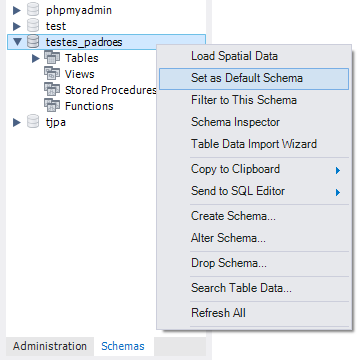
\includegraphics[scale=0.8]{imagens/cap04SelecionandoEsquema}
    \\\textbf{Fonte:} Elaborada pelo autor
    \label{fig:cap04SelecionandoEsquema}
\end{figure}
\FloatBarrier

Com a base \texttt{testes\_padroes} configurada como padrão, expanda-a e em \destaque{\textit{Tables}} clique com o botão direito e escolha \destaque{\textit{Create Table...}}. Vamos criar agora uma tabela que vai armazenar os dados de teste que iremos mexer durante este Capítulo. Preencha \destaque{\textit{Table Name:}} com ``pais'' (sem as aspas). \textit{Pais} é país, mas vamos omitir o acento tudo bem? Deixe os valores padrão nos campos \destaque{\textit{Charset/Collation:}}, \destaque{\textit{Engine:}} e \destaque{\textit{Comments:}}. Logo abaixo, clique duas vezes na primeira linha da coluna \destaque{\textit{Column Name}}. A ferramenta vai preencher o nome da primeira coluna automaticamente com o valor ``idpais''. Edite esse nome e deixe apenas ``id''. O tipo (Datatype) deve ficar como INT (inteiro) e as colunas \texttt{PK} (\textit{primary key}/chave primária), \texttt{NN} (\textit{not null}/não nulo) e \texttt{AI} (auto-increment/auto-incremento) devem ficar marcadas. Essa coluna da tabela será nossa chave primária. Agora vamos às outras colunas. Nossos países terão um nome e uma sigla. Então precisamos criar mais duas colunas, uma com nome de ``nome'' e a outra com nome de ``sigla''. A coluna ``nome'' terá o tipo \inlineSQLCode{VARCHAR(100)}, ou seja, um \inlineSQLCode{VARCHAR} de 100 posições e a coluna ``sigla'' terá o tipo \inlineSQLCode{VARCHAR(2}). Marque essas duas colunas como \texttt{NN}, ou seja, elas terão dados obrigatoriamente quando um país for ser inserido na tabela. Veja como ficou na Figura~\ref{fig:cap04CriandoTabelaPais}.

\FloatBarrier
\begin{figure}[!htbp]
    \centering
    \caption{Criando a tabela ``pais''}
    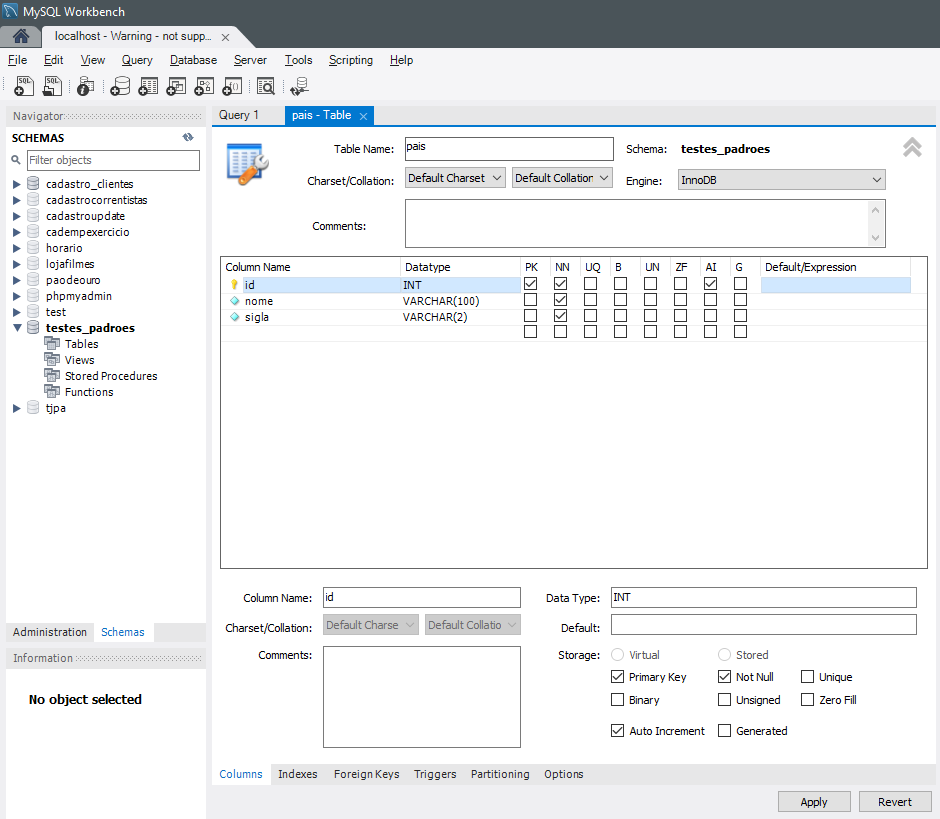
\includegraphics[scale=0.6]{imagens/cap04CriandoTabelaPais}
    \\\textbf{Fonte:} Elaborada pelo autor
    \label{fig:cap04CriandoTabelaPais}
\end{figure}
\FloatBarrier

Feito isso, clique em \destaque{\textit{Apply}}. Um diálogo será aberto para exibir o código SQL que será executado (Listagem~\thechapter.\ref{listagem:projetos/capitulo04/pais.sql}). Clique em \destaque{\textit{Apply}} e depois em \destaque{\textit{Finish}}. Pronto, criamos a nossa tabela para armazenar dados dos países, ela poderá ser vista do lado esquerdo, na aba \destaque{\textit{Schemas}}, dentro da base \texttt{testes\_padroes}. Deixe o Workbench aberto e abra o NetBeans. 

\sqlCode{Instrução \texttt{CREATE TABLE} para a tabela ``pais''}{projetos/capitulo04/pais.sql}

\section{Padrão de Projeto Factory}

Primeiramente, vamos criar um novo projeto no NetBeans, só que agora ele não será um projeto Web, pois o que vamos fazer não precisa ser em um projeto desse tipo. Siga os passos que você está acostumado a fazer ao criar um projeto Java Web, só que desta vez escolha \destaque{\textit{Java with Ant}} na categoria e \destaque{\textit{Java Application}} nos tipos de projeto. Dê o nome de ``PadroesEmPratica'' para o projeto. Não se esqueça de marcar a opção \destaque{\textit{Use Dedicated Folder for Storing Libraries}}.

Como iremos conectar no banco de dados MariaDB, precisamos adicionar no nosso projeto a biblioteca que implementa esse conector. Infelizmente o NetBeans não vem com essa biblioteca pronta para ser usada, então teremos que baixá-la e inseri-la no projeto. Para isso, primeiro baixe o arquivo \texttt{.jar} da bibliteca no endereço \url{NOME}. Com o arquivo baixado, clique com o botão direito no nó \destaque{\textit{Libraries}} e escolha a opção \destaque{\textit{Add Library...}}. No diálogo que foi aberto, clique em \destaque{\textit{Create...}}. No diálogo que vai se abrir, preencha \destaque{\textit{Library Name:}} com ``MariaDB-ConnectorJ-3.0.6'' (ou o nome que você quiser) e em \destaque{\textit{Library Type}} deixe ``Class Libraries'' e clique em \destaque{\textit{OK}}. Mais um diálogo será aberto. Clique no botão \destaque{\textit{Add JAR/Folder...}} e procure pelo arquivo \texttt{.jar} da biblioteca que acabou de baixar. Antes de selecioná-lo, certifique-se que do lado direito do diálogo de abertura de arquivo a opção \destaque{\textit{Copy to Libraries Folder:}} esteja marcada para que o arquivo seja copiado para dentro do nosso projeto. Após essa conferência, selecione o arquivo e clique em \destaque{\textit{Add JAR/Folder}}. Ao clicar nesse botão, um alerta perguntará se você que criar um diretório na pasta de bibliotecas do projeto, clique em \destaque{\textit{Yes}}. Agora clique no botão \destaque{\textit{OK}} do diálogo \destaque{\textit{Customize Library}} e, agora que a biblioteca foi criada, selecione-a no diálogo \destaque{\textit{Add Library}} e clique no botão \destaque{\textit{Add Library}}. Perceba que ao fazer isso, um aparecerá um novo nó dentro da pasta \destaque{\textit{Libraries}} do projeto com o nome da bibliteca que foi criada e adicionada.

A partir de agora, podemos conectar ao banco de dados a partir do nosso código. Como você deve saber, para que possamos usar um banco de dados em Java, nós usamos uma especificação chamada \textit{Java Database Connectivity} (JDBC). Essa especificação deve ser implementada pelos fabricantes dos SGBDs, permitindo assim que os programas feitos em Java possam se comunicar com estes SGBDs. Normalmente, esses pacotes que implementam o JDBC são chamados de ``Drivers JDBC'' e são obtidos nos sites dos fabricantes dos SGBDs.

A questão agora é: ``Como conectar no banco de dados?''. Para que possamos conectar no MariaDB, existem uma série de ``comandos'' que precisamos fazer cada vez que queremos estabelecer uma conexão. Você, como desenvolvedor, sabe que uma boa prática de programação é encapsular trechos de código que fazem uma determinada tarefa em funções e que as funções em Java são chamadas de métodos.

Legal, mas e o que o tal do ``padrão de projeto'' tem haver com isso? Ou melhor, o que é um padrão de projeto? O termo padrão de projeto (\textit{design pattern} em inglês) foi criado por Christopher Alexander \cite{Alexander1977} na década de 1970 para designar soluções de sucesso para problemas recorrentes na área da arquitetura. Alexander definiu nessa época uma série de padrões que apresentavam soluções padrão para problemas que aconteciam de forma corriqueira, sendo que uma série de padrões correlatos foram o que podemos chamar de linguagem de padrões. A partir do termo cunhado por Alexander, alguns programadores começaram a criar padrões de projeto para a computação, iniciando esse trabalho do domínio da programação orientada a objetos.

O livro ``Padrões de Projeto: Soluções Reutilizáveis de Software Orientado a Objetos'' \cite{Gamma2000} é a referência básica para os padrões de projeto criados para resolver problemas relacionados ao desenvolvimento orientado a objetos. A partir de agora, quando você ler ``padrão de projeto'', entenda que estarei falando de padrões relacionados ao desenvolvimento de software orientado a objetos, tudo bem? Sendo assim, o primeiro padrão que iremos aprender se chama \textit{Factory} (fábrica). 

Vamos entender o contexto do padrão. Imagine que no seu programa você precisa criar e utilizar um determinado tipo de objeto muitas e muitas vezes e que este objeto precisa ser inicializado com uma série de valores, sendo que esses valores normalmente são sempre os mesmos. Assim, cada vez que você instância esse objeto, você precisa executar uma determinada quantidade de código. Como resolver isso? Criar um método que faça essa tarefa é uma boa solução não é mesmo? Mas em qual classe eu vou escrever esse método? No padrão \textit{Factory}, nós criamos classes especializadas que serão fábricas de objetos e que terão um método que executará a tarefa da fábrica, ou seja, criar um determinado tipo de objeto.

No nosso projeto, um tipo de objeto que usaremos muito, é um objeto que representa a conexão entre nosso programa escrito em Java e o SGBD. Sendo assim, nós precisamos de uma fábrica de conexões! Vamos implementar a fábrica? No projeto que você criou agora a pouco, o NetBeans gerou por padrão um pacote chamado ``padroesempratica'' dentro da pasta \destaque{\textit{Source Packages}}. Crie dentro deste pacote outro com o nome de ``jdbc'' (sem as aspas) e dentro do pacote ``padroesempratica.jdbc'', crie uma classe Java com o nome de ``ConnectionFactory'' (sem as aspas). Essa classe conterá o método que vai fabricar a conexão. Veja o código dela na ListagemListagem~\thechapter.\ref{listagem:projetos/capitulo04/PadroesEmPratica/src/padroesempratica/jdbc/ConnectionFactory.java}.

\javaCode{Uma fábrica de conexões (\texttt{padroesempratica/jdbc/ ConnectionFacotory.java})}{projetos/capitulo04/PadroesEmPratica/src/padroesempratica/jdbc/ConnectionFactory.java}

Copiou o código? Ótimo! Esta classe tem um método estático chamado \texttt{getConnection()} que vai fabricar a conexão para nós e que caso ocorra algum problema, vai lançar uma exceção do tipo SQLException. Toda vez que chamarmos esse método, ele vai retornar uma nova conexão para nós e o Driver JDBC apropriado será carregado automaticamente pelo \texttt{DriverManager}. 

Agora precisamos testar esse método para ver se não está havendo nenhum erro. Clique novamente com o botão direito no pacote ``padroesempratica'' e crie um novo pacote chamado ``testes''. Dentro do pacote ``padroesempratica.testes'', crie uma classe chamada ``TesteConnectionFactory''. Como você deve saber, para que uma classe em Java possa ser executada, nós precisamos implementar o método \inlineJavaCode{main(...)} com uma determinada assinatura. O que vamos fazer no método \inlineJavaCode{main(...)} da classe ``TesteConnectionFactory'' é tentar criar uma conexão e ver se nenhum erro é retornado. Na Listagem~\thechapter.\ref{listagem:projetos/capitulo04/PadroesEmPratica/src/padroesempratica/testes/TesteConnectionFactory.java} você pode ver o código desta classe.

\javaCode{Classe para teste de conexão (\texttt{padroesempratica/testes/ TesteConnectionFactory.java})}{projetos/capitulo04/PadroesEmPratica/src/padroesempratica/testes/TesteConnectionFactory.java}

Copie o código para a classe e salve o arquivo. Para executarmos apenas uma classe que tem o método \inlineJavaCode{main(...)}, basta clicar com o botão direito no editor e escolhe a opção \destaque{\textit{Run File}}, ou então, com o arquivo aberto no editor, usar o atalho \texttt{<Shift+F6>}. Fazendo isso, a classe vai ser compilada e executada pelo NetBeans. Se tudo estiver correto, você verá na saída a mensagem ``Conexão criada com sucesso!''. Deu erro? Verifique se o código da classe \texttt{ConnectionFactory} está correto e se a senha do usuário \texttt{root}, definida dentro do método \inlineJavaCode{getConnection()} está correta. No nosso caso, ela é vazia. Agora que está tudo certo, vamos simular um erro. Entre na classe \texttt{ConnectionFactory} e coloque uma senha inválida (terceiro parâmetro do método \inlineJavaCode{getConnection(...)} de \texttt{DriverManagaer}) para o usuário \texttt{root}, por exemplo, ``123''. Volte na classe de testes e execute-a novamente (\texttt{<Shift+F6>}). Gerou um erro não foi? A mensagem ``Erro ao tentar criar a conexão!'' deve ter sido exibida, seguida de várias linhas que explicam o erro ocorrido. A primeira linha dos erros diz que o acesso foi negado para o usuário ``root@localhost'' não foi? Por que aconteceu isso? Porque a senha está errada! Volte na fábrica de conexões e coloque a senha correta (vazia). Teste novamente. Agora deve estar tudo certo.

Legal, temos uma fábrica de conexões, mas do que adianta uma fábrica de alguma coisa se a gente não usar o que é fabricado? Vamos para o próximo padrão, onde iremos organizar uma camada de persistência para nossa aplicação e usaremos a fábrica de conexões para viabilizar a comunicação entre nossa aplicação e o SGBD.


\section{Padrão de Projeto \textit{Data Access Object} (DAO)}

Quando temos o nosso primeiro contato com JDBC, normalmente nos é ensinado a colocar todo o código SQL que vai executar uma determinada operação em um método que trata o ``clique'' de um botão. Sendo assim, imagine uma interface gráfica de uma aplicação \textit{desktop} (em Swing) onde poderíamos criar, alterar e/ou excluir países. Quando implementamos o botão responsável por criar um novo país, somos ensinados a inserir todo o código SQL para fazer isso, sendo que esse código é implementado usando uma instrução \inlineSQLCode{INSERT}. O mesmo aconteceria para os botões alterar e excluir. Será que essa é a melhor solução? Será que a classe que implementa nossa interface gráfica tem que ter essa responsabilidade, ou seja, lidar com SQL? E se por algum motivo nós quiséssemos usar o código para criar um novo país em alguma outra janela? Teríamos que copiar o código de inserção novamente? Tenho certeza que para essa última pergunta você já deve ter respondido mentalmente que ``NÃO!'', pois podemos criar métodos que executariam essa operação, mas então te pergunto: Como fazer isso?

Para resolver esse problema, existe um padrão de projeto onde a ideia é isolar todo acesso ao banco de dados em classes que seriam responsáveis em fazer a comunicação entre a aplicação Java, ou qualquer aplicação escrita usando uma linguagem orientada a objetos, e o banco de dados. Esse padrão se chama \textit{Data Access Object} (DAO), sendo este um dos mais famosos. Vamos aprender como implementá-lo?

Um objeto do tipo DAO deve ter a capacidade de executar as operações básicas sobre uma determinada tabela de um banco de dados. Essas operações são comumente chamadas de ``CRUD'' que vem de ``\textit{Create, Read, Update e Delete}'' (Criar, Ler, Atualizar e Excluir). Praticamente cada tabela do nosso banco de dados terá no lado da aplicação uma classe implementada que representará um registro da tabela (tabela ``pais'', classe Pais) por meio de um objeto do tipo em questão, além de ter uma classe DAO que vai manipular esses objetos. Como precisamos definir essas quatro operações básicas que cada DAO vai conter, vamos criar uma classe abstrata que servirá de modelo.

No pacote ``padroesempratica'', crie um novo pacote chamado ``dao''. Dentro do pacote ``padroesempratica.dao'', crie uma classe chamada ``DAO'' e copie o código apresentado na Listagem~\thechapter.\ref{listagem:projetos/capitulo04/PadroesEmPratica/src/padroesempratica/dao/DAO.java}.

\javaCode{Implementação da classe abstrata DAO (\texttt{padroesempratica/dao/DAO.java})}{projetos/capitulo04/PadroesEmPratica/src/padroesempratica/dao/DAO.java}

Copiou o código? Ótimo! Vamos entendê-lo. Na linha 13 definimos uma classe abstrata\footnote{Classes abstratas não podem ser instanciadas, são usadas como modelos.} chamada DAO que diz que toda classe que for implementá-la deve fornecer um tipo genérico chamado de \texttt{Tipo}. As construções entre \inlineJavaCode{<} e \inlineJavaCode{>} são chamadas de ``Tipos Genéricos'' em Java. Note que o tipo \texttt{Tipo} é usado em todo o corpo da classe. Está confuso? Acalme-se, logo você vai entender.

Na linha 16 é declarada uma variável de instância que referenciará uma conexão, que sempre será obtida usando o método \inlineJavaCode{getConnection()} definido na linha 39. Observe que poderíamos ter declarado essa conexão como \inlineJavaCode{protected}, mas vamos deixá-la como \inlineJavaCode{private} e usar o método \inlineJavaCode{getConnection()} para obtê-la. Na linha 49 é definido o método para fechar a conexão, afinal, sempre depois de usarmos uma conexão, precisamos fechá-la.

Veja que no construtor da classe a conexão é obtida usando a fábrica que criamos na Seção anterior! Esse construtor será executado quando instanciarmos os objetos das classes que estenderem esse DAO, então, quando criarmos nossos objetos DAO, uma conexão com o banco de dados será estabelecida.

A partir da linha 62 são definidos todos os métodos CRUD deste DAO genérico. Note que temos dois métodos que correspondem à parte ``R'' do CRUD, onde um obtém todas as entidades cadastradas e outro obtém apenas uma usando como base seu identificador.

Com o DAO genérico pronto, vamos implementar a classe que vai representar a tabela ``pais''. Crie um novo pacote chamado ``entidades'' dentro do pacote ``padroesempratica''. Dentro do pacote ``padroesempratica.entidades'', crie uma classe chamada ``Pais'' (sem as aspas). Os objetos dessa classe representarão registros da tabela ``pais'', sendo assim, precisamos que essa classe tenha os mesmos atributos da tabela correspondente. Lembre-se que na tabela ``pais'' nós definimos três colunas: id (\inlineSQLCode{INT}), nome (\inlineSQLCode{VARCHAR}) e sigla (\inlineSQLCode{VARCHAR}). Na nossa classe, iremos usar o tipo \inlineJavaCode{int} como tipo correspondente ao \inlineSQLCode{INT} da tabela. Para o tipo \inlineSQLCode{VARCHAR}, usaremos \inlineJavaCode{String}. Veja na Listagem~\thechapter.\ref{listagem:projetos/capitulo04/parciais/Pais.java} como deve ficar a implementação parcial da classe \texttt{Pais}.

\javaCode{Implementação parcial da classe Pais (\texttt{padroesempratica/entidades/Pais.java})}{projetos/capitulo04/parciais/Pais.java}

Tenho certeza que você se lembra da discussão sobre o padrão JavaBeans não é mesmo? Onde foi dito que devemos expor ao mundo ``fora da classe'' os atributos que nós queremos que possam ser configurados e obtidos por seus utilizadores? Da primeira vez que falamos sobre isso, nós implementamos manualmente cada método \texttt{set} e \texttt{get} correspondente a um campo privado não foi? Como essa tarefa é muito corriqueira, o NetBeans tem uma funcionalidade que faz isso automaticamente para nós. Com a classe implementada, como exibido na Listagem~\thechapter.\ref{listagem:projetos/capitulo04/parciais/Pais.java}, clique com o botão direito no editor e escolha \destaque{\textit{Insert Code...}}. Ao clicar nesta opção, uma pequena lista com o nome de \destaque{\textit{Generate}} será exibida no editor. Nessa lista, escolha a opção \destaque{\textit{Getter and Setter...}}. Adivinhe o que vamos fazer? Gerar os métodos \texttt{get} e \texttt{set} para cada campo da classe! Fazendo isso, um diálogo será exibido, mostrando todos os campos privados da classe. Marque cada um dos campos clicando na caixa de seleção correspondente, ou então, a classe inteira e clique no botão \destaque{\textit{Generate}}. Veja o que aconteceu! A IDE gerou o código dos \texttt{gets} e \texttt{sets} para nós! Segue na Listagem~\thechapter.\ref{listagem:projetos/capitulo04/PadroesEmPratica/src/padroesempratica/entidades/Pais.java} o código completo da classe Pais.

\javaCode{Implementação da classe Pais (\texttt{padroesempratica/ entidades/Pais.java})}{projetos/capitulo04/PadroesEmPratica/src/padroesempratica/entidades/Pais.java}

Muito legal não é mesmo? Agora que temos a classe que representa a estrutura da tabela ``pais'' da nossa base de dados, vamos implementar nosso primeiro DAO concreto, ou seja, uma classe que vai estender a classe abstrata DAO. Novamente, no pacote ``padroesempratica.dao'', crie uma classe chamada ``PaisDAO'' (sem as aspas). Essa classe irá lidar com os objetos do tipo \texttt{Pais}, fazendo a ponte entre nossos objetos e o banco de dados. Com a classe criada, copie o código apresentado na Listagem~\thechapter.\ref{listagem:projetos/capitulo04/parciais/PaisDAOP1.java}.

\javaCode{Implementação parcial da classe PaisDAO (\texttt{padroesempratica/dao/PaisDAO.java})}{projetos/capitulo04/parciais/PaisDAOP1.java}

Veja que nosso \texttt{PaisDAO} vai estender \texttt{DAO}, informando como tipo a classe \texttt{Pais} (\texttt{DAO<Pais>}). Ao copiar o código, você perceberá que o NetBeans vai reclamar, dizendo que tem um erro na classe. O nome da classe ficará destacado em vermelho. Passe o mouse por cima do nome e aguarde. Será exibida a causa do erro. No erro, é dito que a classe \texttt{PaisDAO} não implementa todos os métodos abstratos da classe \texttt{DAO} e isso é verdade, visto que como estamos estendendo a classe \texttt{DAO}, precisamos implementar todos os métodos abstratos que foram definidos nela e ainda não fizemos isso. Teríamos então que implementar manualmente todos os métodos marcados como abstratos na classe \texttt{DAO}. Ao invés de fazermos isso manualmente, o NetBeans pode nos ajudar novamente. Veja que na linha do erro, à esquerda, é mostrada uma pequena lâmpada com uma bolinha vermelha. Clique nela. Ao clicar, o NetBeans vai listar as alternativas que ele pode executar para resolver o erro. Veja a Figura~\ref{fig:cap04ImplementacaoAutomatica}.

\FloatBarrier
\begin{figure}[!htbp]
    \centering
    \caption{Implementando automaticamente os métodos abstratos de DAO}
    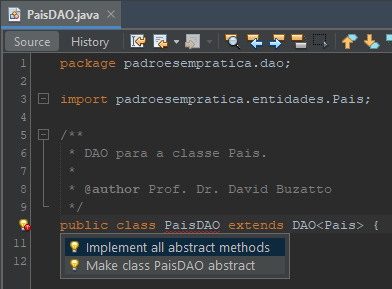
\includegraphics[scale=1]{imagens/cap04ImplementacaoAutomatica}
    \\\textbf{Fonte:} Elaborada pelo autor
    \label{fig:cap04ImplementacaoAutomatica}
\end{figure}
\FloatBarrier

Clique na opção \destaque{\textit{Implement all abstract methods}} e, novamente, como num passe de mágica, o NetBeans gera todo o esqueleto da classe para nós, criando uma implementação padrão para cada método abstrato da classe \texttt{DAO}. Mesmo ao fazer isso, o NetBeans continua reclamando que existe um erro. Nesse caso, é dito que é lançada uma exceção no construtor padrão\footnote{O construtor padrão é o construtor que não tem nenhum parâmetro.}. Você se lembra que lá no \texttt{DAO} genérico nós temos um construtor que cria a conexão e que ele lança uma \texttt{SQLException}? Pois bem, quando criamos um objeto de uma determinada classe, o construtor da superclasse da classe em questão a primeira coisa que será executada. Como estendemos \texttt{DAO} em \texttt{PaisDAO}, ao tentarmos instanciar um objeto do tipo \texttt{PaisDAO}, o construtor de \texttt{PaisDAO} será executado, além do construtor de \texttt{DAO}, que é sua superclasse. Como o construtor de \texttt{DAO} lança uma exceção caso ocorra algum problema, nós precisamos ou tratar ou dizer que o construtor de \texttt{PaisDAO} também lança esse tipo de exceção. Nós iremos usar a segunda abordagem. Para isso, basta implementar o construtor padrão de \texttt{PaisDAO} e dizer que ele lança esse tipo de exceção. Sendo assim, segue na Listagem~\thechapter.\ref{listagem:projetos/capitulo04/parciais/PaisDAOP2.java} a implementação que temos até agora da classe \texttt{PaisDAO}.

\javaCode{Implementação parcial da classe PaisDAO com o construtor padrão (\texttt{padroesempratica/dao/PaisDAO.java})}{projetos/capitulo04/parciais/PaisDAOP2.java}

Muito bom! Até agora preparamos toda o esqueleto do nosso \texttt{PaisDAO}, mas SQL que é bom, nada. Vamos agora implementar nosso primeiro método do CRUD, o ``salvar''. Antes de implementar o método ``salvar'', importe a classe \texttt{java.sql.PreparedStatement}. Na Listagem~\thechapter.\ref{listagem:projetos/capitulo04/parciais/PaisDAOSalvar.java} pode ser vista a implementação do método \texttt{salvar} da classe \texttt{PaisDAO}.

\javaCode{Implementação do método ``salvar'' da classe PaisDAO (\texttt{padroesempratica/dao/PaisDAO.java})}{projetos/capitulo04/parciais/PaisDAOSalvar.java}

Vamos analisar o código para ver o que está acontecendo. Na linha 20 está definida a assinatura do método. O método \texttt{salvar} recebe um parâmetro do tipo \texttt{Pais}, sendo que os dados do objeto passado nesse parâmetro serão persistidos no banco de dados. Nas linhas 22 e 23 é definida a instrução \inlineSQLCode{INSERT} do banco de dados. Como a coluna \texttt{id} da tabela \texttt{pais} foi definida como auto-incremento, nós não precisamos fornecê-la. Ao invés de definirmos manualmente os valores das colunas nome e sigla, perceba que utilizamos sinais de interrogação, indicando que no lugar de cada ponto de interrogação será trocado pelo valor correto. Na linha 25 é criado um \texttt{PreparedStatement} a partir da conexão do \texttt{DAO} usando o código SQL que foi definido nas linhas 22 e 23. Na linha 26, o primeiro parâmetro do código SQL (primeiro ponto de interrogação) é ``trocado'' pelo valor retornado pelo método \inlineJavaCode{getNome()} do objeto referenciado por \texttt{obj} que é do tipo \texttt{Pais}. A mesma coisa acontece na linha 27, onde o segundo parâmetro do código SQL (segundo ponto de interrogação) é ``trocado'' pelo valor retornado pelo método \inlineJavaCode{getSigla()}. Com o \texttt{PreparedStatement} configurado, na linha 29 mandamos que seja executado o \texttt{PreparedStatement}. Por fim, na linha 30, fechamos o \texttt{PreparedStatement}. Fácil não é?

Vamos testar? No pacote ``padroesempratica.testes'', crie uma classe chamada \texttt{TestePaisDAO} e copie o código da Listagem~\thechapter.\ref{listagem:projetos/capitulo04/PadroesEmPratica/src/padroesempratica/testes/TestePaisDAO.java}.

\javaCode{Código de teste para o PaisDAO (\texttt{padroesempratica/ testes/TestePaisDAO.java})}{projetos/capitulo04/PadroesEmPratica/src/padroesempratica/testes/TestePaisDAO.java}

Copiou o código? Execute a classe (botão direito no arquivo, \destaque{\textit{Run File}} ou \texttt{<Shift+F6>}). Se tudo estiver correto, a classe será compilada e executada e nenhum erro será emitido. Fazendo isso, um novo registro na tabela ``pais'' será inserido. Vamos confirmar isso? No MySQL Workbench deve haver um editor SQL já aberto. Se não houver, abra um clicando no ícone com uma folha com a sigla SQL e um sinal de \texttt{+}. Confirme também se a base de dados ``testes\_padroes'' está configurado como padrão ou está ativa. No editor, digite \inlineSQLCode{SELECT * FROM pais;} e clique no botão que tem um desenho de um raio na barra de ferramentas da aba do editor. O código SQL digitado será executado e o resultado será exibido logo abaixo. Veja a Figura~\ref{fig:cap04ExecucaoSelect}.

\FloatBarrier
\begin{figure}[!htbp]
    \centering
    \caption{Fazendo uma consulta do MySQL Workbench}
    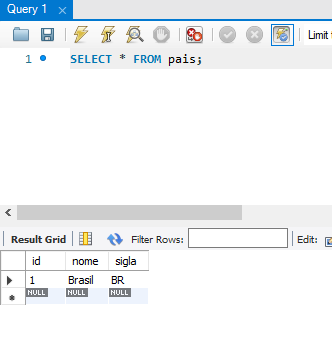
\includegraphics[scale=1]{imagens/cap04ExecucaoSelect}
    \\\textbf{Fonte:} Elaborada pelo autor
    \label{fig:cap04ExecucaoSelect}
\end{figure}
\FloatBarrier

Muito bem! Nosso método \texttt{salvar} de \texttt{PaisDAO} está funcionando corretamente. Vamos analisar o código da Listagem~\thechapter.\ref{listagem:projetos/capitulo04/PadroesEmPratica/src/padroesempratica/testes/TestePaisDAO.java}. Entre as linhas 16 e 18 instanciamos e configuramos um objeto do tipo \texttt{Pais}. O nome desse país é \texttt{Brasil} e a sigla é \texttt{BR}. Na linha 20, declaramos uma referência do tipo \texttt{PaisDAO} que foi inicializada com \inlineJavaCode{null}. Como todo o código dos métodos do \texttt{DAO} podem lançar uma exceção do tipo \texttt{SQLException}, temos que usar um bloco \inlineJavaCode{try}. Na linha 24 instanciamos o \texttt{PaisDAO} e na linha 25 passamos o objeto do tipo \texttt{Pais} que criamos para o método ``salvar'' do \texttt{DAO}, que por sua vez vai executar o código SQL que definimos. Caso ocorra algum problema durante a execução de uma dessas duas linhas, o \inlineJavaCode{catch} que ouve exceções do tipo \texttt{SQLException} captura o erro e manda mostrar esses problemas dando um \inlineJavaCode{printStackTrace()} no objeto que representa a exceção. Por fim, temos um bloco \inlineJavaCode{finally} que trata do fechamento da conexão. Sempre quando usarmos um \texttt{DAO}, precisamos fechar sua conexão quando terminarmos de usar. Na linha 31 verifica-se se o \texttt{dao} aponta para \inlineJavaCode{null}. Se não apontar, tenta fechar a conexão, que também pode lançar uma exceção do tipo \texttt{SQLException} e que é tratada dentro do bloco \inlineJavaCode{try} que está aninhado no \inlineJavaCode{finally}.

Agora que já criamos e testamos nosso primeiro método do \texttt{PaisDAO}, vamos implementar o restante dos métodos. Os métodos de pesquisa (``R'' do CRUD) serão um pouco diferente, sendo assim, eu os discutirei depois. Vamos lá, copie o restante do código para que seu \texttt{PaisDAO} fique igual ao da Listagem~\thechapter.\ref{listagem:projetos/capitulo04/PadroesEmPratica/src/padroesempratica/dao/PaisDAO.java}.

\javaCode{Implementação da classe PaisDAO (\texttt{padroesempratica/ dao/PaisDAO.java})}{projetos/capitulo04/PadroesEmPratica/src/padroesempratica/dao/PaisDAO.java}

Não se esqueça de importar as classes \texttt{java.sql.ResultSet}, \texttt{java.util.ArrayList} e \texttt{java.util.List}. Para finalizar essa seção, vamos discutir o código da Listagem~\thechapter.\ref{listagem:projetos/capitulo04/PadroesEmPratica/src/padroesempratica/dao/PaisDAO.java}. O método \inlineJavaCode{listarTodos()} retorna uma lista que pode conter apenar objetos do tipo \texttt{Pais}. Essa lista que será retornada é instanciada e inicializada na linha 72. Neste momento, temos a lista de objetos do tipo \texttt{Pais}, só que ela ainda está vazia. Na linha 75, cria-se o \texttt{PreparedStatement} com o SQL que foi definido na linha 73 e, na linha 75, executamos o \texttt{PreparedStatement} usando o método \inlineJavaCode{executeQuery()}, que retorna um objeto do tipo \texttt{ResultSet}. Os objetos do tipo \texttt{ResultSet} representam os resultados que são retornados em consultas SQL (instrução \inlineSQLCode{SELECT}). Na linha 78 usamos um \inlineJavaCode{while}, que é executado enquanto \inlineJavaCode{rs.next()} retornar \inlineJavaCode{true}. Na primeira vez que \inlineJavaCode{rs.next()} é invocado, o ponteiro de registros do \texttt{ResultSet} passa a apontar para o primeiro resultado obtido na consulta. Dentro do \inlineJavaCode{while}, entre as linhas 80 e 83, nós criamos um objeto do tipo \texttt{Pais} e configuramos seus dados a partir dos dados obtidos no \texttt{ResultSet}, usando o método apropriado para cada tipo de cada coluna. Na linha 85, o objeto \texttt{Pais} que acabou de ser criado e configurado é inserido na lista. O corpo do \inlineJavaCode{while} é repetido até que \inlineJavaCode{rs.next()} retorne \inlineJavaCode{false}, ou seja, quando todos os resultados da consulta foram obtidos. Nesse ponto, temos a lista de objetos completa. Nas linhas 89 e 90 são fechados o \texttt{ResultSet} e o \texttt{PreparedStatement}. Por fim, na linha 92, a lista com os objetos do tipo \texttt{Pais} é retornada.

Note que o método \inlineJavaCode{obterPorId( int id )} tem uma implementação muito parecida com o método \inlineJavaCode{listarTodos()}, só que no caso do \texttt{obterPorId}, apenas um objeto pode ser retornado, visto que cada registro da tabela \texttt{pais} tem um identificador específico. Caso o \texttt{id} passado como parâmetro não represente um registro da tabela \texttt{pais}, o método retorna \inlineJavaCode{null}.

Agora, como exercício, modifique a classe \texttt{TestePaisDAO} para testar todos os métodos que foram implementados. Verifique se todos estão corretos usando o MySQL Workbench para comparar os resultados obtidos. Tente entender a implementação de cada método do CRUD. Não fez o exercício? Então faça! Ele não é opcional.

Viu só que legal? Com tudo isso que fizemos, conseguimos isolar toda a camada de persistência da nossa aplicação. Para cada tabela nova que tivermos na base de dados, precisamos implementar a classe correspondente à tabela (que chamamos de entidade) e a classe DAO que vai manipular os objetos da classe criada e fazer o intercâmbio entre o mundo orientado a objetos com o mundo relacional. Essa comunicação entre objetos e o modelo relacional é chamada de Object-Relational Mapping (ORM). Existem alguns \textit{frameworks} que automatizam esse processo, gerando todo o código SQL automaticamente para nós. Infelizmente não teremos tempo para aprendê-los. Um desses \textit{frameworks} é o Hibernate.

\begin{saibaMais}
    Quer saber mais sobre ORM? Dê uma olhada nesses \textit{links}: \url{http://pt.wikipedia.org/wiki/Mapeamento_objeto-relacional}, \url{http://en.wikipedia.org/wiki/Object-relational_mapping}, \url{http://www.hibernate.org/}
\end{saibaMais}

Estamos quase acabando! Vamos para o último padrão de projeto.


\section{Padrão de Projeto \textit{Model-View-Controller} (MVC)}


O padrão MVC é um padrão muito utilizado no desenvolvimento de aplicações que utilizam linguagens orientadas a objetos. Este padrão ajuda os desenvolvedores a separar as regras de negócio da aplicação, ou seja, as regras de como os dados devem se armazenados, qual a ordem que devem ser gravados etc., da lógica de apresentação desses dados, ou seja, como eles serão exibidos aos usuários do sistema. Essa separação se dá utilizando três camadas: 

\begin{itemize}

    \item \textbf{\textit{Model} (Modelo):} A camada \textit{Model} é usada para organizar como os dados são armazenados e gerenciados dentro da aplicação. No exemplo que construímos durante este Capítulo, as classes \texttt{Pais} e \texttt{PaisDAO} fazem parte do modelo;
    
    \item \textbf{\textit{View} (Visualização):} Essa camada organiza os recursos utilizados para exibir ao usuário os dados que são gerenciados pela camada de modelo;
    
    \item \textbf{\textit{Controller} (Controle):} A camada \textit{Controller}, como o próprio nome já diz, é responsável por controlar o fluxo de execução da aplicação.
    
\end{itemize}

A partir dessas definições, nós podemos ver nitidamente, nos exemplos que estamos construindo desde o início do livro, qual recurso faz parte de cada camada. A entidade Pais faz parte do modelo. Uma JSP faz parte da visualização, pois é usada pelo usuário tanto para inserir dados no sistema quanto para visualizá-los. Os Servlets que construímos fazem parte do controle, pois são eles que recebem os dados, os utilizam usando a camada de modelo e decidem para onde o fluxo da aplicação deve ser direcionado, por exemplo, uma página JSP que vai exibir a saída gerada por eles.

Essa foi uma pequena introdução do MVC, pois durante Capítulo~\ref{cap:sistemaControleClientes} nós iremos usá-lo extensivamente no projeto que iremos criar. Tenho certeza que você vai achar muito legal e útil! Como de costume, pratique o que você aprendeu durante este Capítulo com as atividades de aprendizagem.


\section{Resumo}

Neste Capítulo demos um passo muito importante na nossa vida como desenvolvedores. Nós aprendemos que existem os chamados ``padrões de projeto'' ou ``\textit{design patterns}'', que são padrões que guiam os desenvolvedores na solução de problemas recorrentes através do uso de soluções de sucesso. Estudamos os padrões \textit{Factory} e DAO implementando exemplos e aprendemos o básico do funcionamento do padrão MVC. No Capítulo~\ref{cap:sistemaControleClientes} iremos implementar um projeto completo usando esses três padrões. 


\section{Exercícios}

\begin{exercicioSemArquivo}{}{}{}
    Defina, com suas palavras, o padrão \textit{Factory}.
\end{exercicioSemArquivo}

\begin{exercicioSemArquivo}{}{}{}
    Defina, com suas palavras, o padrão DAO.
\end{exercicioSemArquivo}

\begin{exercicioSemArquivo}{}{}{}
    Defina, com suas palavras, o padrão MVC.
\end{exercicioSemArquivo}


\section{Projetos}

\begin{projetoSemArquivo}{}{}{}
    Da mesma forma que fizemos para a tabela \texttt{pais}, crie uma tabela na base de dados \texttt{testes\_padroes}, usando o MySQL Workbench, com o nome de ``fruta''. Essa tabela deve ter como colunas um campo identificador (\inlineSQLCode{INT}), um campo que armazenará o nome da fruta (\inlineSQLCode{VARCHAR}) e um campo para armazenar a cor predominante da fruta (\inlineSQLCode{VARCHAR}). Implemente, no projeto que criamos durante este Capítulo, a entidade \texttt{Fruta} e a classe \texttt{FrutaDAO}. Crie uma classe de testes chamada \texttt{TesteFrutaDAO} para testar os métodos do DAO da fruta. 
\end{projetoSemArquivo}

\begin{projetoSemArquivo}{}{}{}
    Repita o Projeto~\ref{cap:padroesDeProjeto}.1, só que agora para a tabela ``carro''. Um carro deve ter um identificador, um nome (\inlineSQLCode{VARCHAR}), um modelo (\inlineSQLCode{VARCHAR}) e um ano de fabricação (\inlineSQLCode{INT}).
\end{projetoSemArquivo}

\begin{projetoSemArquivo}{}{}{}
    Repita o Projeto~\ref{cap:padroesDeProjeto}.1, só que agora para a tabela ``produto''. Um produto deve ter um identificador, uma descrição (\inlineSQLCode{VARCHAR}) e uma quantidade em estoque (\inlineSQLCode{INT}).
\end{projetoSemArquivo}



%\chapter{Sistema para Controle de Clientes}\label{cap:sistemaControleClientes}
\epigraph{``\textit{É fazendo que se aprende a fazer aquilo que se deve aprender a fazer}''.}{Aristóteles}

\lettrine[lines=4, lhang=0.1, lraise=0, loversize=0.2, findent=0.1em]{\textcolor{corTema}{N}}{ESTE} Capítulo teremos como objetivos entender e realizar a construção de uma aplicação Web em Java completa.


\section{Introdução}

Chegou a hora de colocar em prática tudo o que aprendemos nos Capítulos anteriores com o objetivo de criar uma aplicação Web em Java completa. Iremos passar por todos os passos do desenvolvimento da aplicação para que no Capítulo~\ref{cap:primeiroProjeto}, você possa usar um conjunto de requisitos para desenvolver um sistema sozinho. Vamos começar?


\section{Analisando os Requisitos}

Imagine que fomos contratados para criar um sistema para controle de cadastro de clientes. Esse sistema deve manter vários dados de um cliente: nome, sobrenome, data de nascimento, CPF, e-mail, logradouro, número, bairro, cidade e CEP. O contratante também deseja que seja possível manter um cadastro de cidades e de estados, sendo que as cidades devem ter um nome e um estado, enquanto um estado deve ter um nome e uma sigla. Cada um dos cadastros (cliente, cidade e estado), deve conter as funcionalidades de inserir, alterar e excluir um determinado registro.

Vamos analisar esses requisitos. Primeiramente, vamos identificar os tipos de entidades que farão parte do sistema, fazendo a seguinte pergunta: Quais são os tipos de ``coisas'' que o sistema deve gerenciar? O sistema deve manter um cadastro de Clientes, um cadastro de Cidades e um cadastro de Estados. Sendo assim, identificamos três entidades, ou seja, Cliente, Cidade e Estado.

Cada um desses tipos de entidade tem uma determinada lista de características ou atributos. Vamos organizá-las em uma tabela. Veja essa organização na Tabela~\ref{tab:caracteristicasEntidades}.

\FloatBarrier
\begin{table}[ht]
    \centering
    \caption{Atributos dos tipos de entidade}
	\begin{tabular}{cl}
	    \hline
	        \textbf{Entidade}     & \textbf{Atributos (características)} \\ \hline
	    \multirow{10}{*}{Cliente} & - nome                                 \\
	                              & - sobrenome                            \\
	                              & - data de nascimento                   \\
	                              & - CPF                                  \\
	                              & - e-mail                               \\
	                              & - logradouro                           \\ 
	                              & - número                               \\
	                              & - bairro                               \\
	                              & - Cidade                               \\
	                              & - CEP                                  \\ \hline
	     \multirow{2}{*}{Cidade}  & - nome                                 \\
	                              & - Estado                               \\ \hline
	     \multirow{2}{*}{Estado}  & - nome                                 \\
	                              & - sigla                                \\ \hline
	\end{tabular}
    \\ \vspace{0.2cm}
    \textbf{Fonte:} Elaborada pelo autor
    \label{tab:caracteristicasEntidades}
\end{table}
\FloatBarrier

Sabemos que esses tipos de entidade que foram identificados se tornarão tabelas na nossa base de dados relacional não é mesmo? Cada atributo de cada tipo de entidade se tornará uma coluna na tabela correspondente. Sabemos também que cada registro de uma determinada tabela precisa ser diferenciado dos outros não é mesmo? Para isso analisamos as tabelas até que consigamos identificar as chaves primárias de cada uma delas. Uma chave primária é o conjunto mínimo de um ou mais atributos de um determinado tipo de entidade que garante a unicidade de um registro, sendo assim, precisamos encontrar, na lista de características de cada entidade, uma ou mais características que, usadas em conjunto, garantem que um registro é diferente de outro. Tomemos como exemplo o tipo de entidade Estado. Veja na Tabela~\ref{tab:exemplosEstados} uma lista de registros da tabela \texttt{estado} do nosso provável banco de dados.

\FloatBarrier
\begin{table}[ht]
    \centering
    \caption{Exemplos de registros da tabela ``estado''}
	\begin{tabular}{cc}
	    \hline
	    \multicolumn{2}{l}{\textbf{Tabela: estado}} \\ \hline
	    \textbf{nome}  &       \textbf{sigla}       \\ \hline
	      São Paulo    &             SP             \\ \hline
	    Rio de Janeiro &             RJ             \\ \hline
	     Minas Gerais  &             MG             \\ \hline
	         ...       &            ...             \\ \hline
	\end{tabular}
    \\ \vspace{0.2cm}
    \textbf{Fonte:} Elaborada pelo autor
    \label{tab:exemplosEstados}
\end{table}
\FloatBarrier

O que diferencia um estado de outro? Se usarmos os atributos \texttt{nome} e \texttt{sigla}, nós sempre teremos um estado diferente do outro, ou seja, não seria permitido a criação de um novo estado que tivesse o mesmo nome \textbf{e} a mesma sigla do que ume estado que já existe na tabela, concorda? Agora pense, e se usarmos apenas o \texttt{nome} ou somente a \texttt{sigla}, qual seria suficiente? Temos então três opções para definir a chave primária dessa tabela. Podemos usar \texttt{nome} \textbf{e} \texttt{sigla}, somente \texttt{nome} ou somente \texttt{sigla}. Dentre essas três opções, qual ou quais são as que têm o menor conjunto de atributos? Somente \texttt{nome} ou somente \texttt{sigla}, correto? Como temos duas opções, podemos escolher qualquer uma delas, desde que, para o cenário ou ``minimundo'' que está sendo modelado, um desses atributos garanta a unicidade de tupla. Vamos dizer que nós escolhemos a opção de definir a chave primária da tabela usando o atributo \texttt{sigla}. Legal, agora sabemos que um Estado é diferenciado do outro pela sua sigla, então não pode existir mais de um registro com a mesma sigla.

Agora temos outro problema: o desempenho do banco de dados. Quando criarmos a tabela \texttt{cidade}, esta vai ter que referenciar a tabela \texttt{estado}, usando uma coluna que vai ter o mesmo tipo da coluna que representa a chave primária da tabela \texttt{estado}. Essa coluna, como você deve se lembrar, é denominada chave estrangeira. Como cada estado tem uma sigla de dois caracteres, sempre que um estado for referenciado em um registro da tabela \texttt{cidade}, essa referência vai ter que ter o mesmo valor do registro contido na tabela sigla. Apesar de essa abordagem funcionar, nós podemos atacar esse problema de outra forma. Podemos definir que a coluna \texttt{sigla} tem valor único (\textit{unique}) nos registros da tabela \texttt{estado} e então criar uma chave primária que contém apenas um número. Essa chave primária é chamada de chave artificial, ou \textit{surrogate}, sendo que normalmente é chamada de \texttt{id} (identificador). Note que como o próprio nome diz, essa chave é artificial. O que vai garantir a unicidade dos registros é a configuração de cada uma das colunas.

O que ganhamos com isso? Ganhamos desempenho, pois estamos usando números para referenciar colunas de outras tabelas, não Strings. Imagine definir a chave primária de um Cliente como CPF. Ao precisarmos referenciar um cliente em outra tabela, digamos uma tabela de \texttt{pedidos}, precisaríamos ter uma cópia do CPF do cliente em cada pedido, gastando cerca de 11 a 14 caracteres (um CPF é no formato 000.000.000-00), ao passo que poderíamos usar apenas um número! Veja, se cada caractere ocupar 4 bytes em disco/memória, um CPF de 11 dígitos (só os números) ocupará 44 bytes (352 bits), enquanto um número inteiro provavelmente ocupará 4 ou 8 bytes (32 ou 64 bits). Pense nas implicações! Sabendo de tudo isso, podemos partir para o projeto do banco de dados.


\section{Projetando Banco de Dados}

Não irei documentar aqui todo o processo de projeto do banco de dados, que vai desde a análise dos requisitos, passando pela criação do DER (Diagrama Entidade-Relacionamento) até a implementação do modelo físico, pois este não é o objetivo deste livro, mas note que no desenvolvimento de um sistema esses passos são normalmente realizados. Iremos partir diretamente para a implementação do modelo físico. Antes de criarmos o código escrito em \textit{Structured Query Language} (SQL) para a criação da estrutura da nossa base de dados, vamos organizar os atributos das nossas tabelas –que são baseadas nas características dos tipos de entidade– e especificar suas características. Veja a Tabela~\ref{tab:detalhesTabelas}.

\FloatBarrier
\begin{table}[ht]
    \centering
    \caption{Detalhamento das colunas de cada tabela}
	\begin{tabular}{cllc}
	    \hline
	         \textbf{Tabela}      & \textbf{Coluna}                         & \textbf{Tipo}               & \textbf{É único?} \\ \hline
	    \multirow{11}{*}{cliente} & \texttt{id\textsuperscript{*}}          & \inlineSQLCode{INT}         &         x         \\
	                              & \texttt{nome}                           & \inlineSQLCode{VARCHAR(45)} &                   \\
	                              & \texttt{sobrenome}                      & \inlineSQLCode{VARCHAR(45)} &                   \\
	                              & \texttt{dataNascimento}                 & \inlineSQLCode{DATE}        &                   \\
	                              & \texttt{cpf}                            & \inlineSQLCode{VARCHAR(14)} &         x         \\
	                              & \texttt{email}                          & \inlineSQLCode{VARCHAR(60)} &                   \\
	                              & \texttt{logradouro}                     & \inlineSQLCode{VARCHAR(50)} &                   \\
	                              & \texttt{numero}                         & \inlineSQLCode{VARCHAR(6)}  &                   \\
	                              & \texttt{bairro}                         & \inlineSQLCode{VARCHAR(30)} &                   \\
	                              & \texttt{cep}                            & \inlineSQLCode{VARCHAR(9}   &                   \\
	                              & \texttt{cidade\_id\textsuperscript{**}} & \inlineSQLCode{INT}         &                   \\ \hline
	     \multirow{3}{*}{cidade}  & \texttt{id\textsuperscript{*}}          & \inlineSQLCode{INT}         &         x         \\
	                              & \texttt{nome}                           & \inlineSQLCode{VARCHAR(30)} &                   \\
	                              & \texttt{estado\_id\textsuperscript{**}} & \inlineSQLCode{INT}         &                   \\ \hline
	     \multirow{3}{*}{estado}  & \texttt{id\textsuperscript{*}}          & \inlineSQLCode{INT}         &         x         \\
	                              & \texttt{nome}                           & \inlineSQLCode{VARCHAR(30)} &                   \\
	                              & \texttt{sigla}                          & \inlineSQLCode{VARCHAR(2)}  &         x         \\ \hline
	    \multicolumn{4}{l}{\textsuperscript{\texttt{ *}} chave primária}                                                      \\ \hline
	    \multicolumn{4}{l}{\textsuperscript{\texttt{**}} chave estrangeira}                                                   \\ \hline
        \multicolumn{4}{l}{todas as colunas são não nulas (\texttt{NOT NULL})}                                                \\ \hline
	\end{tabular}
    \\ \vspace{0.2cm}
    \textbf{Fonte:} Elaborada pelo autor
    \label{tab:detalhesTabelas}
\end{table}
\FloatBarrier

Usei o MySQL Workbench para criar um diagrama do nosso modelo físico. Veja como ficou na Figura~\ref{fig:cap05ModeloFisico}.

\FloatBarrier
\begin{figure}[!htbp]
    \centering
    \caption{Diagrama do modelo físico da base de dados}
    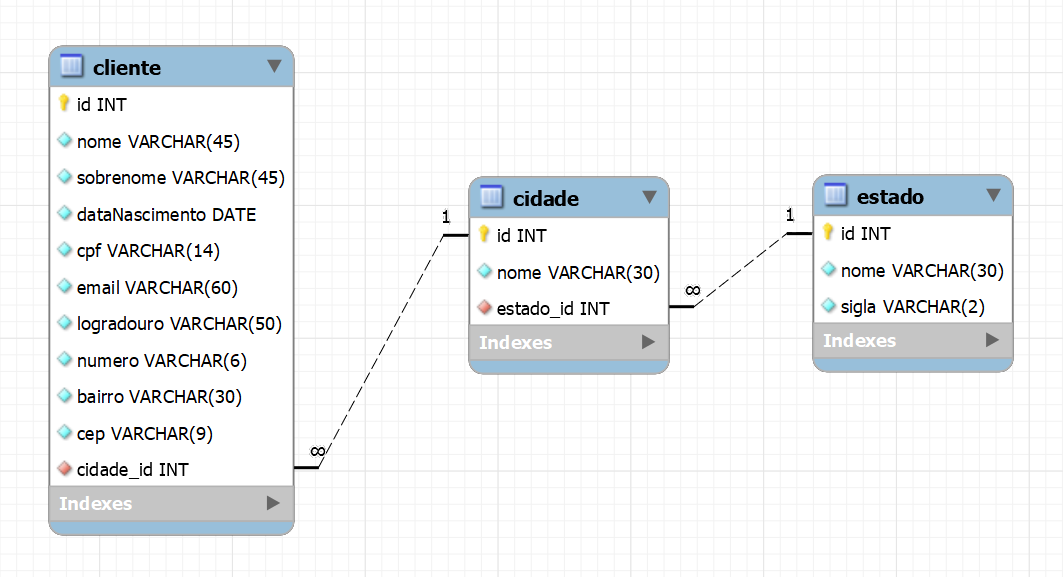
\includegraphics[scale=0.5]{imagens/cap05ModeloFisico}
    \\\textbf{Fonte:} Elaborada pelo autor
    \label{fig:cap05ModeloFisico}
\end{figure}
\FloatBarrier

Vamos agora implementar o banco de dados. No MySQL Workbench, crie uma nova base de dados com o nome de \texttt{cadastro\_clientes} como feito na Seção~\ref{sec:preparandoAmbiente}. Com a base criada, torne-a padrão, abra uma aba para digitar código SQL e copie o código da Listagem~\thechapter.\ref{listagem:projetos/capitulo05/banco/estado.sql} no editor e execute o \textit{script}.

\sqlCode{\textit{Script} SQL para criação da tabela ``estado''}{projetos/capitulo05/banco/estado.sql}

Faça o mesmo processo para a Listagem~\thechapter.\ref{listagem:projetos/capitulo05/banco/cidade.sql} e para a Listagem~\thechapter.\ref{listagem:projetos/capitulo05/banco/cliente.sql}.

\sqlCode{Script SQL para criação da tabela ``cidade''}{projetos/capitulo05/banco/cidade.sql}

\sqlCode{Script SQL para criação da tabela ``cliente''}{projetos/capitulo05/banco/cliente.sql}

Ao fazer esses três passos, temos nossas três tabelas criadas dentro da base de dados. Expanda o banco \texttt{cadastro\_clientes} e então expanda o nó \destaque{\textit{Tables}}. Lá dentro estarão as três tabelas criadas. Muito bem, terminamos a implementação do banco. Vamos agora criar um diagrama de classes para representar cada uma das nossas entidades, que serão mapeamentos das nossas tabelas no mundo orientado a objetos.


\section{Criando o Diagrama de Classes}

Para criar nosso diagrama de classes UML eu usei a ferramenta Astah UML. Existem diversas ferramentas de modelagem gratuítas. Infelizmente o Astah não poussi mais esse tipo de versão desde 2018. Você pode usar qualquer uma caso queria fazer a modelagem, mas ela não é obrigatória. Como já disse cada tabela do nosso banco de dados vai ter uma representação na nossa aplicação. Essa representação, como você já sabe, é criada usando classes. No diagrama de classes da Figura~\ref{fig:cap05DiagramaClasses}, você pode ver as três classes que representam nossas entidades. Note que cada classe contém uma série de atributos privados, denotados pelo sinal de ``\texttt{-}'', que representam as colunas da tabela e que o acesso a esses atributos é feito usando os métodos \texttt{get} e \texttt{set} correspondentes, omitidos no diagrama.

\FloatBarrier
\begin{figure}[!htbp]
    \centering
    \caption{Diagrama de classes das entidades}
    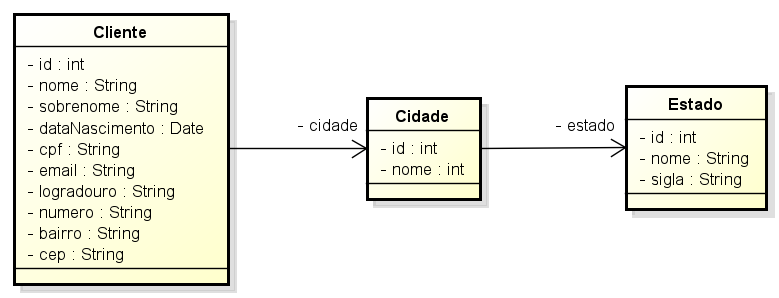
\includegraphics[scale=0.6]{imagens/cap05DiagramaClasses}
    \\\textbf{Fonte:} Elaborada pelo autor
    \label{fig:cap05DiagramaClasses}
\end{figure}
\FloatBarrier

Outro detalhe é que criei apenas o diagrama das classes que são as entidades do sistema, não me preocupando com as outras classes que nosso sistema conterá. Novamente, como no exemplo do nosso banco de dados, em um sistema de verdade, normalmente são desenvolvidos diagramas de classes muito mais completos e complexos, dependendo do nível de representação que se deseja, bem como outros tipos de diagramas UML que forem necessários. Com tudo isso pronto, podemos partir para o desenvolvimento do sistema propriamente dito! Novamente, essa não é a nossa preocupação neste livro.


\section{Construindo o Sistema}

Antes de qualquer coisa precisamos fazer um ajuste no GlassFish, pois ele precisa que todas as biblitecas/APIs que não fazem parte do Java \textit{Standard Edition} (SE), ou do Java/Jakarta EE, sejam fornecidas à ele. Para isso, faça uma cópia do arquivo \texttt{.jar} do \textit{driver} JDBC do MariaDB para o diretório:

\destaque{\texttt{C:\textbackslash Users\textbackslash <SeuUsuário>\textbackslash glassfish5\textbackslash glassfish\textbackslash domains\textbackslash domain1\textbackslash lib\textbackslash}}

Com isso, nossa aplicação poderá usar o \textit{driver} quando estiver implantada no servidor, mas note que ainda precisaremos configurá-lo do projeto, visto que ele será necessário no processo de \textit{build}.

Agora nossa tarefa será criar o projeto no NetBeans. Para isso, abra o NetBeans e crie um novo projeto do tipo Java Web com o nome de ``CadastroClientes'' (sem as aspas). Siga os passos que você tem seguido em todos os projetos criados, além de, é claro, configurar a bibliteca do \textit{driver} JDBC do MariaDB, como descrito no Capítulo~\ref{cap:padroesDeProjeto}. Em \destaque{\textit{Source Packages}}, crie o pacote ``\texttt{cadastroclientes}'' (sem as aspas) e, dentro dele, os pacotes ``controladores'', ``dao'', ``entidades'', ``jdbc'' e ``testes'' dentro do pacote ``cadastroclientes''. Em \destaque{\textit{Web Pages}}, crie os diretórios ``\texttt{css}'' e ``\texttt{formularios}'' (sem acento) e dentro deste, crie os diretórios ``\texttt{cidades}'', ``\texttt{clientes}'' e ``\texttt{estados}''. Apague o arquivo \texttt{index.html} e crie um arquivo JSP chamado \texttt{index.jsp}. Veja na Figura~\ref{fig:cap05EstruturaProjeto} como deve ficar a estrutura do projeto. Ignore os pacotes \texttt{...filtros} e \texttt{...servicos} por enquanto!

\FloatBarrier
\begin{figure}[!htbp]
    \centering
    \caption{Estrutura do projeto}
    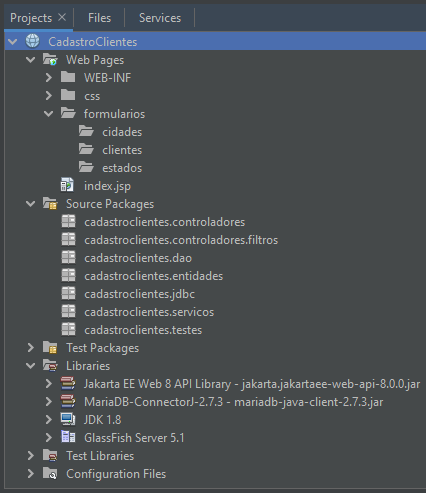
\includegraphics[scale=0.7]{imagens/cap05EstruturaProjeto}
    \\\textbf{Fonte:} Elaborada pelo autor
    \label{fig:cap05EstruturaProjeto}
\end{figure}
\FloatBarrier

Com a estrutura configurada, vamos agora copiar algumas classes do projeto ``PadroesEmPatrica'' que criamos no Capítulo~\ref{cap:padroesDeProjeto}. Para isso abra esse projeto, se ainda não estiver aberto, no NetBeans. Expanda o pacote ``\texttt{padroesempratica.jdbc}'', clique com o botão direito no arquivo ``\texttt{ConnectionFactory.java}'' e escolha \destaque{\textit{Copy}}. Volte ao projeto ``CadastroClientes'', clique com o botão direito no pacote ``cadastroclientes.jdbc'', escolha \destaque{\textit{Paste}} e então \destaque{\textit{Refactor Copy...}}. Um diálogo será aberto. Clique no botão \destaque{\textit{Refactor}}. O arquivo será copiado para o projeto e as alterações que forem necessárias fazer no arquivo, como mudar a cláusula \inlineJavaCode{package}, serão feitas pelo NetBeans. Faça o mesmo processo para o arquivo ``DAO.java'' contido no pacote ``pradoesempratica.dao'' do projeto ``PadroesEmPratica'', copiando-o no pacote ``cadastroclientes.dao'' do projeto ``CadastroClientes''. Talvez o NetBeans aponte um erro no arquivo depois da cópia. Para corrigir, abra o arquivo no editor e altere o \inlineJavaCode{import} que está com problema. 

Outro detalhe é que precisamos mudar a URL da nossa fábrica de conexões para fazer com que as conexões criadas sejam relativas à base de dados \texttt{cadastro\_clientes}. Para isso, abra o arquivo ``\texttt{ConnectionFactory.java}'' do pacote\linebreak%
``\texttt{cadastroclientes.jdbc}'' e mude a URL de:

\destaque{\texttt{jdbc:mariadb://localhost/testes\_padroes}}

Para:

\destaque{\texttt{jdbc:mariadb://localhost/cadastro\_clientes}}

Agora vamos preparar toda a camada de persistência. No pacote\linebreak%
``\texttt{cadastroclientes.entidades}'', crie três classes: ``\texttt{Estado}'', ``\texttt{Cidade}'' e ``\texttt{Cliente}'' (sem as aspas). Nas três listagens a seguir estão listados os códigos-fonte das três classes. Note que estou omitindo os gets e os sets, mas isso não significa que eles não devam existir. Fica por sua conta criá-los ok? Não se esqueça de fazer isso!

\javaCode{Entidade ``Estado''\newline%
Arquivo: \texttt{cadastroclientes/entidades/Estado.java}}{projetos/capitulo05/CadastroClientes/src/java/cadastroclientes/entidades/Estado.java}

\javaCode{Entidade ``Cidade''\newline%
Arquivo: \texttt{cadastroclientes/entidades/Cidade.java}}{projetos/capitulo05/CadastroClientes/src/java/cadastroclientes/entidades/Cidade.java}

\javaCode{Entidade ``Cliente''\newline%
Arquivo: \texttt{cadastroclientes/entidades/Cliente.java}}{projetos/capitulo05/CadastroClientes/src/java/cadastroclientes/entidades/Cliente.java}

Com as entidades prontas, vamos criar os DAOs. No pacote ``\texttt{cadastroclientes.dao}'', crie três classes: ``\texttt{EstadoDAO}'', ``\texttt{CidadeDAO}'' e ``\texttt{ClienteDAO}''. O código-fonte de cada uma dessas classes é apresentado nas listagens a seguir.

\javaCode{Código da classe ``EstadoDAO''\newline%
Arquivo: \texttt{cadastroclientes/dao/EstadoDAO.java}}{projetos/capitulo05/CadastroClientes/src/java/cadastroclientes/dao/EstadoDAO.java}

\javaCode{Código da classe ``CidadeoDAO''\newline%
Arquivo: \texttt{cadastroclientes/dao/CidadeDAO.java}}{projetos/capitulo05/CadastroClientes/src/java/cadastroclientes/dao/CidadeDAO.java}

\javaCode{Código da classe ``ClienteDAO''\newline%
Arquivo: \texttt{cadastroclientes/dao/ClienteDAO.java}}{projetos/capitulo05/CadastroClientes/src/java/cadastroclientes/dao/ClienteDAO.java}

Quantos códigos hein? Copiou tudo? Crie algumas classes de teste no pacote\linebreak%
``\texttt{cadastroclientes.teste}'' e teste a persistência de cada entidade. Com isso, terminamos a parte da persistência do nosso projeto.

Agora nós vamos começar a implementar as visualizações e os controladores. Nossa aplicação terá três \textit{links} no \texttt{index.jsp}, sendo que cada \textit{link} levará a um determinado cadastro. Cada cadastro vai conter uma página principal onde todos os itens desse cadastro serão exibidos e onde poderão ser alterados, excluídos ou então poderemos cadastrar um novo item.

Vamos começar pelo cadastro de estados. Na pasta ``\texttt{estados}'' dentro da pasta\linebreak%
``\texttt{formularios}'', crie um arquivo JSP com o nome de ``\texttt{listagem.jsp}'' (sem as aspas). Nesse arquivo vão ser listados todos os estados, portanto precisamos obter esses estados de alguma forma. Você se lembra que nos nossos DAOs existe um método chamado \inlineJavaCode{listarTodos()} que retorna todos os registros de uma determinada tabela? Nós não vamos usar esse método diretamente no JSP, então vamos criar uma classe de serviços que vai instanciar o DAO, gerar a lista e fechar a conexão para nós. Nos pacotes de código-fonte, crie um novo pacote dentro do ``\texttt{cadastroclientes}'' chamado ``\texttt{servicos}'' (sem o ``ç''). Nesse pacote, crie uma classe chamada ``\texttt{EstadoServices}'' (sem as aspas). Essa classe vai ter apenas um método, chamado \inlineJavaCode{getTodos()}, que retornará uma lista de estados. Veja o código-fonte dela na Listagem~\thechapter.\ref{listagem:projetos/capitulo05/CadastroClientes/src/java/cadastroclientes/servicos/EstadoServices.java}.

\javaCode{Código-fonte da classe de serviços para Estados\newline%
Arquivo: \texttt{cadastroclientes/servicos/EstadoServices.java}}{projetos/capitulo05/CadastroClientes/src/java/cadastroclientes/servicos/EstadoServices.java}

Criamos essa classe para que ela encapsule todo o processo de obtenção da lista de estados. Note que é no método \inlineJavaCode{getTodos()} que o \texttt{EstadoDAO} vai ser instanciado e gerenciado.

Agora que temos o JSP que vai obter a lista de estados para nós, além de gerenciar o DAO, nós podemos implementar o nosso arquivo de listagem de estados. Abra o arquivo \texttt{/formularios/estados/listagem.jsp} e copie o código da Listagem~\thechapter.\ref{listagem:projetos/capitulo05/CadastroClientes/src/java/cadastroclientes/servicos/EstadoServices.java}.

\htmlCode{Código da listagem de Estados\newline%
Arquivo: \texttt{/formularios/estados/listagem.jsp}}{projetos/capitulo05/CadastroClientes/web/formularios/estados/listagem.jsp}

Perceba que a identação do código foi feita com dois espaços para economizar espaço nas listagens, mas você pode manter os quatro espaços usados por padrão.

Vamos analisar o código, detalhando as novidades que aparecerem. Nas linhas 3 e 4 usamos a \textit{tag} \inlineHTMLCode{<c:set>} para configurar no escopo da página dois valores que usaremos no código. Um deles, chamado de \texttt{cp} será o caminho do contexto da aplicação, obtido através da instrução \inlineHTMLCode{${pageContext.request.contextPath}}. Essa instrução da EL retornará no nosso caso o valor \texttt{/CadastroClientes}, pois é esse o contexto da aplicação configurado na criação do projeto. Faremos dessa forma para que, independente do contexto, ele seja obtido apropriadamente. Estamos fazendo isso para que possamos configurar sempre caminhos absolutos para os nossos recursos, evitando problemas de referenciamento relativo. Poderemos acessar esse valor agora usando a construção \inlineHTMLCode{${cp}}. O mesmo acontece na linha 4, onde o valor \texttt{processaEstados?acao=preparar} é configurado na variável \texttt{prefixo}. Veremos o motivo adiante.

Entre as linhas 21 e 25, criamos um link que aponta para o arquivo\linebreak%
\texttt{/CadastroClientes/formularios/estado/novo.jsp} –que ainda não implementamos– e que será o formulário responsável em criar um novo estado. Perceba que usamos a variável de página \texttt{cp} para obter o contexto da aplicação. Este mesmo código é repetido entre as linhas 65 e 69. Na linha 27, abrimos a \textit{tag} de uma tabela e, até a linha 36, criamos seu cabeçalho. Na linha 31, usamos a \textit{tag} \inlineHTMLCode{<jsp:useBean>} para instanciar um objeto do tipo \texttt{EstadoServices}, que contém o método que vamos usar para obter a lista de estados. Demos o nome de \texttt{servicos} para essa instância. Na linha 44, usamos um \inlineHTMLCode{<c:forEach>} para iterar sobre a lista retornada pelo método \inlineJavaCode{getTodos()} da instância \texttt{servicos}. Note que a chamada do método \inlineJavaCode{getTodos()} é somente \inlineJavaCode{todos}, pois seguimos o padrão JavaBeans nas ELs como você deve se lembrar. Essa chamada é feita usando EL no atributo \texttt{items}. No atributo \texttt{var}, damos o nome da variável que vai armazenar a instância atual durante a iteração, no caso, \texttt{estado}. Entre as linhas 45 e 59 nós definimos o código que será gerado a cada iteração do \inlineHTMLCode{<c:forEach>}, que corresponde à uma linha da tabela. As três primeiras colunas da tabela são fáceis de entender, entretanto a quarta e a quinta mudam um pouco. Entre as linhas 49 e 53, a coluna é formada por um \textit{link} que aponta para \texttt{\textbf{\textcolor{Fuchsia}{\$\{cp\}}}/\textbf{\textcolor{ForestGreen}{\$\{prefixo\}}}Alteracao\&id=\${estado.id}}, que após ser processado gerará o caminho \texttt{\textbf{\textcolor{Fuchsia}{/CadastroClientes}}/\textbf{\textcolor{ForestGreen}{processaEstados?acao=prepararar}}Alteracao\&}\linebreak%
\texttt{id=AlgumId}. Veja que usamos \textcolor{Fuchsia}{\texttt{\textbf{cp}}} e \textcolor{ForestGreen}{\texttt{\textbf{prefixo}}}, sendo que, respetivamente serão substituídas por \textcolor{Fuchsia}{\texttt{\textbf{/CadastroClientes}}} e \textcolor{ForestGreen}{\texttt{\textbf{processaEstados?acao=prepararar}}}. Note que estamos codificando na URL duas variáveis. A primeira, chamada ``acao'', vai informar para o Servlet que vai estar mapeado para \texttt{/processaEstados} o que queremos fazer, no caso, ``prepararAlteracao''. A segunda variável, chamada ``\texttt{id}'' vai conter o identificador do estado daquela linha da tabela, ou seja, queremos alterar um estado que tem um determinado \texttt{id}. O mesmo acontece entre as linhas 54 e 59, mudando a ação para ``prepararExclusao''. Sei que pode estar um pouco confuso, mas na hora que terminarmos todos os arquivos do cadastro de estados tudo isso vai ficar fácil de entender, não se preocupe.

Note que deixei a linha 13 por último. Nela usamos a \textit{tag} \inlineHTMLCode{<link>} para referenciar um arquivo de folhas de estilos. Nos exemplos dos Capítulos anteriores nós usamos estilos declarados dentro dos arquivos HTML e/ou JSP usando a \textit{tag} \inlineHTMLCode{<style>}. A partir de agora iremos separar os estilos em arquivos e é por isso que foi usada a \textit{tag} \inlineHTMLCode{<link>} para a pontar para \texttt{\$\{cp\}/css/estilos.css}. Note novamente o uso da variável \texttt{cp}!. Vamos criar esse arquivo? Na pasta ``\texttt{css}'' dentro de \destaque{\textit{Web Pages}} -que criamos quando preparamos o projeto- clique com o botão direito sobre ele e escolha \destaque{\textit{New}}. Provavelmente o item que queremos não estará visível, então escolha \destaque{\textit{Other...}}. Escolha \destaque{\textit{Web}} na categoria e em \destaque{\textit{File Types}} escolha \destaque{\textit{Cascading Style Sheet}}. Clique em próximo e dê o nome de ``estilos'' ao arquivo. Copie o código da Listagem~\thechapter.\ref{listagem:projetos/capitulo05/CadastroClientes/web/css/estilos.css}. neste arquivo.

\cssCode{Arquivo de estilos da aplicação\newline%
Arquivo: \texttt{/css/estilos.css}}{projetos/capitulo05/CadastroClientes/web/css/estilos.css}

Execute o projeto e aponte o navegador para a página de listagem para ver como está ficando. Se você já tiver alguns estados previamente cadastrados via SQL, vai ver que eles aparecerão na tabela. Vamos agora criar nosso formulário para criar estados. Na pasta \texttt{/formularios/estados}, crie um arquivo JSP chamado ``novo'' (sem as aspas). O código-fonte do arquivo pode ser visto na Listagem~\thechapter.\ref{listagem:projetos/capitulo05/CadastroClientes/web/formularios/estados/novo.jsp}.

\htmlCode{Formulário de cadastro de novos Estados\newline%
Arquivo: \texttt{/formularios/estados/novo.jsp}}{projetos/capitulo05/CadastroClientes/web/formularios/estados/novo.jsp}

Salve o arquivo e veja se ele está sendo exibido corretamente no navegador. Acesse-o pelo link ``Novo Estado'' da página de listagem de estados. Vamos analisar o código. Na linha 12 referenciamos o nosso arquivo de estilos. Na linha 20 declaramos a \textit{tag} do formulário. Note que a \texttt{action} está apontando para \texttt{\$\{cp\}/processaEstados} que será a URL que mapearemos o Servlet que tratará os estados. A novidade nesse formulário é o uso de um \textit{input} do tipo \texttt{hidden} (escondido). Esses tipos de \textit{input} são usados para guardar valores que o usuário do sistema não tem acesso diretamente. No nosso caso, esse \textit{input}, que tem o nome de \texttt{acao} e valor \texttt{inserir}, vai indicar ao Servlet que queremos criar um novo estado. Nós precisamos tratar isso na implementação do nosso Servlet ok? Além disso, perceba que utilizamos alguns atributos nos \textit{inputs} para que nosso formulário seja validado antes de ser submetido. Por exemplo, o \textit{input} do atributo nome do estado tem tamanho máximo de 30 caracteres (\texttt{maxlength}) e é obrigatório (\texttt{required}). Como já temos nossa página de listagem e o nosso formulário de criação de estados, está na hora de criarmos o Servlet que vai gerenciar isso. No pacote \texttt{cadastroclientes.controladores}, crie um Servlet com o nome de ``EstadosServlet'' (sem as aspas) e configure o mapeamento dele para ``/processaEstados'' (sem as aspas).

A seguir, na Listagem~\thechapter.\ref{listagem:projetos/capitulo05/CadastroClientes/src/java/cadastroclientes/controladores/EstadosServlet.java} é apresentado o código completo da classe \texttt{EstadosServlet}.

\javaCode{Código-fonte do Servlet ``EstadosServlet''\newline%
Arquivo: \texttt{cadastroclientes/controladores/EstadosServlet.java}}{projetos/capitulo05/CadastroClientes/src/java/cadastroclientes/controladores/EstadosServlet.java}

Perceba que a linha que contém o código para a configuração do \textit{encoding} do \texttt{request} que estávamos usando até agora foi removida pois, para não precisarmos ter essa configuração em cada Servlet, criaremos um Filtro para realizar essa ação padrão para nós. Os filtros das aplicações Web em Java são componentes que podem atuar antes e/ou depois de requisições à outros componentes da aplicação, inclusive outros filtros. Para isso, crie primeiramente o pacote ``\texttt{filtros}'' dentro do pacote\linebreak%
``\texttt{controladores}''. No pacote ``\texttt{filtros}', crie uma nova classe chamada\linebreak%
``\texttt{ConfigurarEncodingFilter.java}'' e copie o código apresentado na Listagem~\thechapter.\ref{listagem:projetos/capitulo05/CadastroClientes/src/java/cadastroclientes/controladores/filtros/ConfigurarEncodingFilter.java}. Note que poderíamos ter criado o filtro usando a opção apropriada nos tipos de arquivo disponíveis no NetBeans, entretanto, nosso filtro é bastante simples e todo o código inserido pelo NetBeans quando criamos usando o \textit{template} é praticamente desnecessário para a nossa necessidade, sendo assim, faremos manualmente.

\javaCode{Filtro de configuração de encoding padrão\newline%
Arquivo: \texttt{cadastroclientes/controladores/filtros/ConfigurarEncoding-\newline%
Filter.java}}{projetos/capitulo05/CadastroClientes/src/java/cadastroclientes/controladores/filtros/ConfigurarEncodingFilter.java}

Veja que na linha 17 é usada anotação \inlineJavaCode{@WebFilter} que será responsável em indicar ao servidor de aplicações que essa classe é um Filtro. O nome do filtro, indicado pelo atributo \texttt{filterName}, é usado para indentificar o filtro, enquanto o atributo \texttt{urlPatterns} indica em quais URLs esse filtro será aplicado. No nosso caso, queremos que todas as requisições da aplicação passem por ele, então usamos o padrão \texttt{/*}, onde o asterisco denota ``tudo''. O método \inlineJavaCode{doFilter()} realiza a atividade de filtragem, sendo que será executado antes das requisições. Queremos sempre definir a codificação para \texttt{UTF-8} para padronizarmos o \textit{encoding} que a aplicação utiliza, evitando problemas com caracteres acentuados e símbolos especiais. Isso é feito na linha 28. Na linha 29, dá-se a chance de outros filtros que porventura tenham sido criados atuarem na requisição.

Voltando ao EstadosServlet apresentado na Listagem~\thechapter.\ref{listagem:projetos/capitulo05/CadastroClientes/src/java/cadastroclientes/controladores/EstadosServlet.java}, copie todo o código e execute o projeto. Acesse a listagem de estados e clique para criar um novo estado. Preencha o formulário e salve. O novo estado será salvo e a listagem aparecerá novamente. Teste a inserção de estados com nomes que contém palavras acentuadas, por exemplo, ``São Paulo'' e verifique se os caracteres acentuados estão sendo persistidos apropriadamente. Como exercício, tente entender o que está acontecendo no Servlet. Todo o código apresentado já foi estudado nos exemplos anteriores. Perceba que foram tratadas todas as ações possíveis, mas ainda faltam dois arquivos JSP para implementarmos. O \texttt{alterar.jsp} e o \texttt{excluir.jsp}. Vamos fazer isso? Crie um arquivo JSP na pasta \texttt{/formularios/estados} com o nome de ``\texttt{alterar}'' (sem as aspas) e copie o código da Listagem~\thechapter.\ref{listagem:projetos/capitulo05/CadastroClientes/web/formularios/estados/alterar.jsp}.

\htmlCode{Formulário de alteração de Estados cadastrados\newline%
Arquivo: \texttt{/formularios/estados/alterar.jsp}}{projetos/capitulo05/CadastroClientes/web/formularios/estados/alterar.jsp}

As diferenças importantes em relação ao arquivo \texttt{novo.jsp} são poucas. O que foi alterado é o \textit{input} \texttt{hidden} nomeado como \texttt{acao}, que agora tem o valor \texttt{alterar}. Foi criado outro \textit{input} \texttt{hidden} para armazenar o \texttt{id} do estado que será alterado. Note que os valores dos campos são preenchidos usando o atributo ``estado'' que foi configurado no \texttt{request} dentro do Servlet, na seção do código que trata a ação \texttt{prepararAlteracao}.

O arquivo \texttt{excluir.jsp} é bem parecido, só que neste arquivo não precisamos ter campos de entrada para nome e sigla, pois não vamos alterar esses dados. O importante é o \texttt{id}, que novamente vai ser configurado em um campo escondido. Veja na Listagem~\thechapter.\ref{listagem:projetos/capitulo05/CadastroClientes/web/formularios/estados/excluir.jsp} o código do arquivo \texttt{/formularios/estados/excluir.jsp} que você deve criar.

\htmlCode{Formulário de exclusão de Estados cadastrados \newline%
Arquivo: \texttt{/formularios/estados/excluir.jsp}}{projetos/capitulo05/CadastroClientes/web/formularios/estados/excluir.jsp}

Copiou tudo? Teste! Verifique se tudo está funcionando corretamente. Antes de partirmos para os outros cadastros, vamos alterar o \texttt{index.jsp} criando três links, um para cada listagem dos cadastros. O novo código do \texttt{index.jsp} pode ser visto na Listagem~\thechapter.\ref{listagem:projetos/capitulo05/CadastroClientes/web/index.jsp}.

\htmlCode{Código-fonte do ``index.jsp''\newline%
Arquivo: \texttt{/index.jsp}}{projetos/capitulo05/CadastroClientes/web/index.jsp}

Teste o index.jsp e veja que agora ele tem três links para cada um dos cadastros. O que falta agora para terminarmos nosso projeto é implementar todos os JSPs dos outros cadastros, bem como seus respectivos Servlets e classes de serviço. A seguir, vou listar cada um desses arquivos, agrupando-os por tipo de cadastro, sendo que só irei comentar as linhas que contenham código que ainda não utilizamos ou que precisem de alguma explicação. Não se esqueça de testar o projeto sempre que tiver implementado os arquivos necessários para o funcionamento de uma determinada funcionalidade. No cabeçalho de cada listagem é indicado o arquivo em que ela deve estar, sendo assim lembre-se de criá-lo antes! Vamos começar?

\javaCode{Código-fonte da classe de serviços para Cidades\newline%
Arquivo: \texttt{cadastroclientes/servicos/CidadeServices.java}}{projetos/capitulo05/CadastroClientes/src/java/cadastroclientes/servicos/CidadeServices.java}
 
\htmlCode{Código da listagem de Cidades \newline%
Arquivo: \texttt{/formularios/cidades/listagem.jsp}}{projetos/capitulo05/CadastroClientes/web/formularios/cidades/listagem.jsp}

\htmlCode{Formulário de cadastro de novas Cidades \newline%
Arquivo: \texttt{/formularios/cidades/novo.jsp}}{projetos/capitulo05/CadastroClientes/web/formularios/cidades/novo.jsp}

Note que na linha 45 da Listagem~\thechapter.\ref{listagem:projetos/capitulo05/CadastroClientes/web/formularios/cidades/novo.jsp} nós usamos o serviço \inlineJavaCode{getTodos()} da classe \texttt{EstadoServices} para obter todos os estados cadastrados e com isso gerar as opções (\textit{tag} \inlineHTMLCode{<option>}) do \texttt{select} (\textit{combo box}). Note que o valor de cada option é o \texttt{id} associado a determinado estado, enquanto o que aparece ao usuário é a concatenação do nome e da sigla do mesmo estado. O \texttt{id} do estado selecionado será enviado ao Servlet por meio do parâmetro \texttt{idEstado}, configurada no atributo \texttt{name} da \textit{tag} \inlineHTMLCode{<select>}.

\javaCode{Código-fonte do Servlet ``CidadesServlet''\newline%
Arquivo: \texttt{cadastroclientes/controladores/CidadesServlet.java}}{projetos/capitulo05/CadastroClientes/src/java/cadastroclientes/controladores/CidadesServlet.java}

\htmlCode{Formulário de alteração de Cidades cadastradas\newline%
Arquivo: \texttt{/formularios/cidades/alterar.jsp}}{projetos/capitulo05/CadastroClientes/web/formularios/cidades/alterar.jsp}

Na Listagem~\thechapter.\ref{listagem:projetos/capitulo05/CadastroClientes/web/formularios/cidades/alterar.jsp} temos algo muito interessante. Note que construímos nosso \texttt{select} da mesma forma que fizemos na Listagem~\thechapter.\ref{listagem:projetos/capitulo05/CadastroClientes/web/formularios/cidades/novo.jsp}, entretanto precisamos saber qual é o estado que é usado na cidade que será alterada. Para isso, ao usarmos o \inlineHTMLCode{<c:forEach>}, nós comparamos o \texttt{id} de cada estado do cadastro com o \texttt{id} do estado associado à cidade que vai ser alterada. Caso os ids sejam iguais, isso quer dizer que é o estado relacionado à cidade, sendo assim, a \textit{tag} \inlineHTMLCode{<option>} é gerada com um atributo a mais, o \texttt{selected}, que não possui valor. Usando esse atributo, nós dizemos ao navegador que aquele item deve estar selecionado por padrão.

\htmlCode{Formulário de exclusão de Cidades cadastradas \newline%
Arquivo: \texttt{/formularios/cidades/excluir.jsp}}{projetos/capitulo05/CadastroClientes/web/formularios/cidades/excluir.jsp}
 
\javaCode{Código-fonte da classe de serviços para Clientes\newline%
Arquivo: \texttt{cadastroclientes/servicos/ClienteServices.java}}{projetos/capitulo05/CadastroClientes/src/java/cadastroclientes/servicos/ClienteServices.java}
 
\htmlCode{Código da listagem de Clientes \newline%
Arquivo: \texttt{/formularios/clientes/listagem.jsp}}{projetos/capitulo05/CadastroClientes/web/formularios/clientes/listagem.jsp}

\htmlCode{Formulário de cadastro de novos Clientes\newline%
Arquivo: \texttt{/formularios/clientes/novo.jsp}}{projetos/capitulo05/CadastroClientes/web/formularios/clientes/novo.jsp}

Na Listagem~\thechapter.\ref{listagem:projetos/capitulo05/CadastroClientes/web/formularios/clientes/novo.jsp} usamos diversos atributos para implementar a validação do formulário do cliente que será cadastrado. No \textit{input} do tipo \texttt{date} (data), apresentado na linha 48, usamos o atributo \texttt{placeholder} para indicar o formato esperado para a data, que no caso é \inlineHTMLCode{"dd/mm/yyyy"}, ou seja, dia com dois dígitos (\texttt{dd}), mês com dois dígitos (\texttt{mm}) e ano com quatro dígitos (\texttt{yyyy}), todos separados por barra. Esse tipo de \textit{input} normaliza o formato da data que será enviado e que receberá como valor. Esse formato é sempre \inlineHTMLCode{"yyyy-mm-dd"}. No \textit{input} do CPF usamos o atributo \texttt{placeholder} para indicar ao usuário o formato esperado e o atributo \texttt{pattern} para validar esse formato. O valor do atributo \texttt{pattern} é uma expressão regular que no nosso caso é \inlineHTMLCode{"\d{3}.\d{3}.\d{3}-\d{2}"}. Cada \texttt{\textbackslash d} indica que ali é esperado um dígito e o valor entre chaves é a quantidade esperada de símbolos. Sendo assim, para o CPF temos três digitos, um ponto, mais três dígitos e um ponto, mais três dígitos, um traço/hífen e mais dois dígitos.

\javaCode{Código-fonte do Servlet ``ClientesServlet''\newline%
Arquivo: \texttt{cadastroclientes/controladores/ClientesServlet.java}}{projetos/capitulo05/CadastroClientes/src/java/cadastroclientes/controladores/ClientesServlet.java}

Note que no início da Listagem~\thechapter.\ref{listagem:projetos/capitulo05/CadastroClientes/src/java/cadastroclientes/controladores/ClientesServlet.java} (linha 36), nós usamos a classe\linebreak%
\inlineJavaCode{java.time.format.DateTimeFormatter} para converter a data inserida pelo usuário no formulário, que vem como texto, para um objeto do tipo \inlineJavaCode{java.sql.Date}. Para fazer essa conversão, precisamos criar o \inlineJavaCode{DateTimeFormatter} com o formato que a data chegará, no caso \inlineJavaCode{"yyyy-MM-dd"}, ou seja, ano com quatro dígitos (\texttt{yyyy}), mês com dois dígitos (\texttt{MM}) e dia com dois dígitos (\texttt{dd}). Com o formatador criado, usamos o método \inlineJavaCode{parse(...)} de \inlineJavaCode{java.time.LocalDate}, sendo que a String com a data que é passada para o método \inlineJavaCode{parse(...)} deve estar no formato especificado no construtor do \inlineJavaCode{DateTimeFormatter}. Ainda, o objeto do tipo \inlineJavaCode{java.time.LocalDate} é usado como parâmetro do método \inlineJavaCode{valueOf(...)} da classe \inlineJavaCode{java.sql.Date} para converter o \inlineJavaCode{java.time.LocalDate} para \inlineJavaCode{java.sql.Date} e configurar no objeto do tipo Cliente que está sendo populado com os dados apropriados.

\htmlCode{Formulário de alteração de Clientes cadastrados\newline%
Arquivo: \texttt{/formularios/clientes/alterar.jsp}}{projetos/capitulo05/CadastroClientes/web/formularios/clientes/alterar.jsp}

Para que possamos apresentar a data de nascimento (tipo java.sql.Date) do cliente que está passando pelo processo de edição em um formato específico, nós usamos a \textit{tag} \inlineHTMLCode{<fmt:formatDate>} (linha 52 da Listagem~\thechapter.\ref{listagem:projetos/capitulo05/CadastroClientes/web/formularios/clientes/alterar.jsp}), que faz parte da JSTL. Note que a TagLib que contém essa \textit{tag} é declarada no início da Listagem~\thechapter.\ref{listagem:projetos/capitulo05/CadastroClientes/web/formularios/clientes/alterar.jsp} usando o prefixo \texttt{fmt}. Na \textit{tag} \inlineHTMLCode{<fmt:formatDate>}, usamos o atributo \texttt{pattern} (padrão) para configurarmos o formato da String que deve ser gerada a partir da data de nascimento do cliente. O atributo \texttt{value} é usado para indicar o objeto da data que faz parte do objeto \texttt{cliente} contido no \texttt{requestScope}, ou seja, o objeto que queremos formatar. O atributo \texttt{var} é usado para indicar o nome da variável usada para armazenar o resultado da formatação, sendo que no caso, configuramos o nome da variável como \texttt{data}. Por fim, o atributo \texttt{scope} é usado para definir o escopo que essa variável vai existir, no caso, cofiguramos para \texttt{page}, ou seja, a variável só vai existir dentro dessa página. A seguir, como valor do input da data de nascimento, usamos a variável \texttt{data}, obtida usando EL na forma \texttt{\$\{data\}}.

\htmlCode{Formulário de exclusão de Clientes cadastrados\newline%
Arquivo: \texttt{/formularios/clientes/excluir.jsp}}{projetos/capitulo05/CadastroClientes/web/formularios/clientes/excluir.jsp}

Veja que no final da Listagem~\thechapter.\ref{listagem:projetos/capitulo05/CadastroClientes/web/formularios/clientes/excluir.jsp} usamos novamente um formatador de datas (\textit{tag} \inlineHTMLCode{<fmt:formatDate>}) para apresentar a data de nascimento do cliente. Note que desta vez o uso do formatador foi simplificado, visto que agora não precisamos inserir a data formatada dentro de um input como fizemos na Listagem~\thechapter.\ref{listagem:projetos/capitulo05/CadastroClientes/web/formularios/clientes/alterar.jsp}. Quando queremos apenas exibir a data formatada, basta usarmos a \textit{tag} \inlineHTMLCode{<fmt:formatDate>} com os atributos ``pattern'' e ``value'' configurados que a data formatada será gerada onde a \textit{tag} foi usada.

Ufa! Quanta coisa! Copiou todos os arquivos? Testou tudo o que você fez? Que bom! Se tudo funcionou, parabéns! Caso tenha dado algum problema, verifique o que pode ter acontecido, principalmente comparando o código que você copiou com o código das listagens. Agora você é capaz de criar uma aplicação Web em Java que contenha cadastros. Muito legal não é mesmo? Com essa bagagem teórica e prática que tivemos neste e nos Capítulos anteriores, nós seremos capazes de trabalhar no projeto que será proposto no Capítulo~\ref{cap:primeiroProjeto}.

\section{Resumo}

Neste Capítulo construímos uma aplicação Web completa que mantém o cadastro de Clientes, Cidades e Estados. Durante o nosso aprendizado, nós usamos os padrões que aprendemos no Capítulo~\ref{cap:padroesDeProjeto} para criar a arquitetura da nossa aplicação, dividindo as responsabilidades entre as classes, bem como usando as camadas propostas no padrão MVC, organizando assim o nosso projeto. 


\section{Projetos}

\begin{projetoSemArquivo}{}{}{}
    Na listagem de clientes, insira uma nova coluna na tabela para apresentar a data de nascimento de cada cliente. Use a \textit{tag} \inlineHTMLCode{<fmt:formatDate>} para formatar a data no formato \texttt{dd/MM/yyyy} (dia com dois dígitos, mês com dois dígitos e ano com quatro dígitos). Não se esqueça de usar a diretiva \texttt{<\%@taglib ... \%>} para configurar a TagLib de formatadores da JSTL. 
\end{projetoSemArquivo}

\begin{projetoSemArquivo}{}{}{}
    No projeto implementado durante o Capítulo, implementamos a validação dos formulários através de diversos atributos dos \textit{inputs}. Como você deve saber, esse tipo de validação pode ser contornado pelo usuário usando a inspeção do código fonte pelas ferramentas do desenvolvedor. Tente criar um mecanismo de validação dos dados fornecidos pelo usuário no cadastro de estados. Caso algum campo não tenha as características necessárias (sigla com mais de dois caracteres, por exemplo), direcione o usuário para uma página de erro, onde deve ser apresentado ao usuário qual erro ocorreu. Nessa página deve existir um botão ``Voltar'', que levará o usuário de volta à listagem de estados.
\end{projetoSemArquivo}

\begin{projetoSemArquivo}{}{}{}
    Crie um mecanismo de validação de dados para o cadastro de cidades, da mesma forma que você fez para o cadastro de estados.
\end{projetoSemArquivo}

\begin{projetoSemArquivo}{}{}{}
    Crie um mecanismo de validação de dados para o cadastro de clientes, da mesma forma que você fez para o cadastro de estados.
\end{projetoSemArquivo}
%\chapter{Primeiro Projeto: Sistema para Locação de DVDs v1.0}\label{cap:primeiroProjeto}
\epigraph{``\textit{Só se conhece o que se pratica}''.}{Barão de Montesquieu}

\lettrine[lines=4, lhang=0.1, lraise=0, loversize=0.2, findent=0.1em]{\textcolor{corTema}{N}}{ESTE} Capítulo aplicaremos o conhecimento adquirido até o momento na construção de uma aplicação Web em Java.


\section{Introdução}

Neste Capítulo será apresentada uma série de requisitos que devem ser usados para criar uma aplicação Web da mesma forma que fizemos no Capítulo~\ref{cap:sistemaControleClientes}. Tudo que será requisitado estará baseado no que já aprendemos, sendo assim, todas as funcionalidades requeridas poderão ser implementadas com recursos já vistos no Capítulo~\ref{cap:sistemaControleClientes}. Note que apesar do projeto ser intitulado como um sistema para locação de DVDs, por enquanto a implementação da locação em si será deixada de lado, pois você a fará no projeto do Capítulo~\ref{cap:segundoProjeto}. Isso se dá porque ainda precisamos aprender mais algumas coisas, principalmente do lado do cliente, para sermos capazes de implementar cadastros que lidem com relacionados muitos-para-muitos.


\section{Apresentação dos Requisitos}

Você foi contratado para criar um sistema para controle de cadastro de DVDs. Esse sistema irá manter apenas o cadastro de DVDs e não irá gerenciar a locação dos mesmos. Os dados que deverão ser mantidos para todos os DVDs são: título, ano de lançamento, ator principal, ator coadjuvante, data de lançamento, duração em minutos, gênero e classificação etária. Os dados dos atores, dos gêneros e das classificações etárias deverão ser mantidos através de cadastros específicos. Um ator deve ter um nome, um sobrenome e uma data de estreia (indica quando foi o primeiro filme do ator). Um gênero deve ter uma descrição. Uma classificação etária deve ter também apenas uma descrição. Cada um dos cadastros (DVD, ator, gênero e classificação etária), deve conter as funcionalidades de criar, alterar e excluir um determinado registro. A página principal da aplicação deve conter um link para cada tipo de cadastro.


\section{Desenvolvimento do Projeto}

O projeto Web que deverá ser criado deve ter o nome de ``LocacaoDVDs''. Configure o projeto para conter as bibliotecas internamente. O pacote de código-fonte base do projeto deve ter o nome de ``\texttt{locacaodvds}''. A estrutura do projeto deve ser igual à estrutura do projeto criado no Capítulo~\ref{cap:sistemaControleClientes}, sendo que, obviamente, o nome das classes e suas respectivas implementações serão diferentes do projeto daquele Capítulo. A base de dados com as tabelas das entidades obtidas a partir da análise dos requisitos na seção anterior deve ter o nome de ``\texttt{locacao\_dvds}''. Note que nos arquivos de código fonte disponibilizados, na pasta deste Capítulo, é fornecido um arquivo do MySQL Workbench com um modelo do cenário apresentado acima. Não se esqueça de que cada entidade deverá conter um identificador. As páginas da aplicação deverão ter sua aparência configurada usando uma folha de estilos, da mesma forma que fizemos no projeto do Capítulo~\ref{cap:sistemaControleClientes}. Personalize os estilos, mudando as cores etc., além de usar imagens ou quaisquer outros artifícios que julgar interessante para mudar a aparência da sua aplicação.


\section{Resumo}

Neste Capítulo foi requisitado que você implementasse uma aplicação Web em Java para gerenciar o cadastro de DVDs de uma locadora (ainda sem a locação), por isso, não há atividades a serem realizadas.

%
%\part{O Que Falta do Básico?}
%\chapter{Introdução à Linguagem JavaScript}\label{cap:javaScript}
\epigraph{``\textit{A vida vai ficando cada vez mais dura perto do topo}''.}{Friedrich Nietzsche}

\lettrine[lines=4, lhang=0.1, lraise=0, loversize=0.2, findent=0.1em]{\textcolor{corTema}{N}}{ESTE} Capítulo temos como objetivo aprender as construções básicas da linguagem de programação JavaScript, vastamente utilizada no desenvolvimento de aplicações Web.

\section{Introdução}

Chegamos a talvez à cereja do bolo, ou à cereja do livro ou então à cereja do desenvolvimento para Web: a linguagem de \textit{script} JavaScript. A primeira coisa que precisamos deixar claro é que Java e JavaScript são duas linguagens diferentes, com sintaxe baseada em C e com construções similares, mas o comum entre as duas para por aqui. A linguagem JavaScript não é uma linguagem orientada a objetos, mas sim baseada em protótipos. Nesse tipo de linguagem não existem classes, mas apenas objetos. Novos objetos são criados a partir de cópias de objetos existentes. O JavaScript ``moderno'', baseado no padrão ECMAScript 2015 (sexta edição), possui algumas construções que lembram àquelas de linguagens orientadas a objetos como classes e herança, mas tudo isso é \textit{syntax sugar} para simplificar coisas que já existiam anteriormente. Outras construções também são suportadas na linguagem como as funções de primeira classe etc.

Neste Capítulo não entraremos em detalhes sobre a história da linguagem e da sua evolução, mas sim no que eu acho útil e fundamental para que possamos começar a usá-la. Iremos ter uma visão geral da linguagem como declaração de variáveis, manipulação do \textit{Document Object Model} (DOM) e requisições assíncronas. Durante o Capítulo serão apresentadas inúmeras caixas do tipo ``Saiba Mais'' com \textit{links} úteis. A maioria desses links serão da \textit{Mozilla Developer Network}\footnote{\url{https://developer.mozilla.org/}} (MDN), uma referência confiável e oficial da maioria, senão de todas, das tecnologias para Web. Sempre fornecerei os \textit{links} da versão em inglês do site, mas se quiser, você pode verificar a versão em português clicando no botão ``\textit{Change language}'' presente em todas as páginas do site. Sinceramente recomendo a leitura em inglês, pois o texto sempre estará completo, atualizado com a terminologia correta.

\begin{saibaMais}
    Quer conhecer um pouco mais da história e dos detalhes da linguagem JavaScript? Veja o \textit{link} \url{https://developer.mozilla.org/en-US/docs/Web/JavaScript}.
\end{saibaMais}

\begin{saibaMais}
    A referência da linguagem JavaScript pode ser acessada pelo \textit{link} \url{https://developer.mozilla.org/en-US/docs/Web/JavaScript/Reference}.
\end{saibaMais}

\begin{saibaMais}
    As documentações e referências das tecnologias e APIs usadas para o desenvolvimento para Web podem ser acessadas pelo \textit{link} \url{https://developer.mozilla.org/en-US/docs/Web/API}.
\end{saibaMais}

\begin{saibaMais}
    Caso deseje fazer um tutorial completo sobre a linguagem, recomendo o ótimo tutorial da própria MDN: \url{https://developer.mozilla.org/en-US/docs/Learn/JavaScript}.
\end{saibaMais}

Antes de começarmos a falar do JavaScript propriamente dito, vamos montar nosso palco, que é um projeto Java para Web. Neste Capítulo ainda faremos a construção dos projetos do zero, mas a partir do próximo focarei apenas nas novidades que serão apresentadas.

Vamos lá. Crie um projeto Java Web com o nome de ``ExemplosEmJavaScript'' da forma que tem feito até aqui. Os passos descritos a seguir são somente estruturais. Os respectivos códigos dos arquivos serão apresentados e explicados posteriormente. Sendo assim, no nó \destaque{\textit{Web Pages}} do projeto:

\begin{itemize}
    \item Remova o arquivo \texttt{index.html};
    \item Crie um JSP chamado \texttt{index.jsp};
    \item Crie uma pasta chamada \texttt{css};
    \item Crie uma pasta chamada \texttt{js} (JavaScript);
    \item Dentro da pasta \texttt{css} crie um arquivo CSS chamado \texttt{estilos.css};
    \item Dentro da pasta \texttt{js} crie 12 arquivos JavaScript, chamados \texttt{exemplo01.js}, \texttt{exemplo02.js}... \texttt{exemplo12.js};
    \item Em \destaque{\textit{Source Packages}} crie os pacotes \texttt{exemplosemjavascript.pojo} e\newline%
    \texttt{exemplosemjavascript.servlets};
    \item No pacote \texttt{exemplosemjavascript.pojo} crie uma classe chamada \texttt{Pessoa};
    \item No pacote \texttt{exemplosemjavascript.servlets} crie os Servlets \texttt{CalculaTabuadaServlet} e \texttt{ListagemPessoasServlet};
    \item Importe e insira no projeto a biblioteca \texttt{Jakarta EE Web 8 API};
    \item Clique com o botão direito do mouse no nó raiz do projeto e escolha o último item do menu de contexto, chamado \destaque{\textit{Properties}};
    \begin{itemize}
        \item Do lado esquerdo, em \destaque{\textit{Categories:}}, clique no item \destaque{CDNJS}, situado dentro do nó \destaque{\textit{JavaScript Libraries}};
        \item Do lado direito, clique no botão \destaque{\textit{Add}};
        \item No diálogo que abriu, intitulado \destaque{\textit{Add CDNJS Library}}, preencha o campo \destaque{\textit{Find:}} com ``\texttt{jquery}'' (sem as aspas) e clique em \destaque{\textit{Search}};
        \item Após a busca na \textit{Content Delivery Network} (CDN) aparecerão diversos componentes na \textit{Graphical User Interface} (GUI). Em \destaque{\textit{Libraries:}} escolha \texttt{jquery}, provavelmente o primeiro item;
        \item Em \destaque{\textit{Files:}} marque a \textit{checkbox} na frente do item \texttt{jquery.min.js} e clique em \destaque{\textit{Add Library}} como na Figura~\ref{fig:cap07AddCDNJSLibrary};
        \FloatBarrier
        \begin{figure}[!htbp]
            \centering
            \caption{Adicionando uma biblioteca JavaScript}
            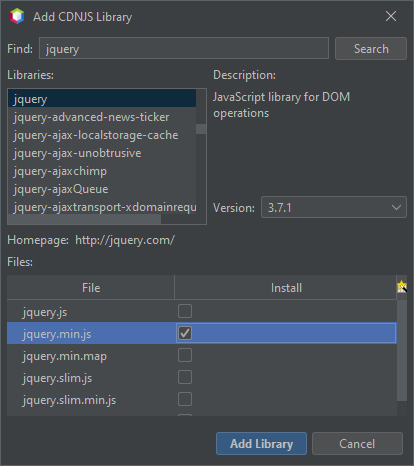
\includegraphics[scale=0.7]{imagens/cap07AddCDNJSLibrary}
            \\\textbf{Fonte:} Elaborada pelo autor
            \label{fig:cap07AddCDNJSLibrary}
        \end{figure}
        \FloatBarrier
        \item Clique em \destaque{OK}. A biblioteca jQuery será baixada e inserida no projeto dentro da pasta \texttt{js/libs/jquery}.
    \end{itemize}
\end{itemize}

Realizando todos os passos descritos anteriormente, você terá um projeto com a estrutura apresentada na Figura~\ref{fig:cap07EstruturaDoProjeto}. Agora vamos começar a preencher cada um dos arquivos e aprender o que está acontecendo em cada um deles.

\FloatBarrier
\begin{figure}[!htbp]
    \centering
    \caption{Estrutura do projeto}
    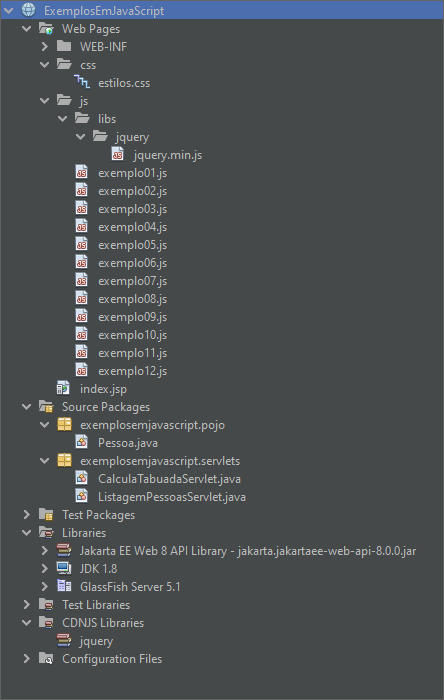
\includegraphics[scale=0.7]{imagens/cap07EstruturaDoProjeto}
    \\\textbf{Fonte:} Elaborada pelo autor
    \label{fig:cap07EstruturaDoProjeto}
\end{figure}
\FloatBarrier

Começaremos com o \texttt{index.jsp} apresentado na Listagem~\thechapter.\ref{listagem:projetos/capitulo07/ExemplosEmJavaScript/web/index.jsp}. Entre as linhas 10 e 22 usamos a \textit{tag} \inlineHTMLCode{<script>} para carregarmos no documento treze arquivos de código JavaScript. Inclusive, essa mesma \textit{tag} pode ser utilizada para inserir código JavaScript no próprio documento. Veremos isso mais adiante. Na linha 10 é carregada a biblioteca jQuery que há alguns anos atrás era absolutamente relevante, mas que hoje em dia tem caído em desuso visto a evolução do JavaScript. Ela será tratada no livro pela sua importância em software legado, por facilitar e padronizar algumas coisas e também, é claro, por preferência minha :D. No restante das linhas são associados os arquivos com os exemplos que aprenderemos. O restante do documento consiste na construção de uma GUI com alguns componentes e \textit{tags} que serão manipulados pelo nosso código em JavaScript. 

Os cinco primeiros exemplos são relativos às construções principais da linguagem. Veja que da linha 30 à 34 temos um parágrafo (\textit{tag} \inlineHTMLCode{<p>}) com um botão dentro (\textit{tag} \inlineHTMLCode{<button>}) e que em seu evento \textit{click}, representado pelo atributo \texttt{onclick}, é registrado uma função tratadora/manipuladora/ouvinte de evento (\textit{event handler} ou \textit{event listener}). Para registrar uma função como tratadora de um determinado evento, basta inserir seu nome no valor do atributo \texttt{onclick} e adicionar, entre os parânteses da mesma, a palavra \texttt{event}. Esse \texttt{event} carregará o objeto do evento que será disparado pela \textit{tag} e ouvido pela função. Essa função precisa estar declarada e implementada em algum lugar. No nosso caso, estará no arquivo \texttt{exemplo01.js}, referenciado acima. Note que como o JavaScript é interpretado, para se poder usar algo, essa ``coisa'' precisa ter sido declarada antes ou as vezes ``vista'' pelo interpretador pela primeira vez, sendo que esse segundo comportamento pode gerar muitos problemas caso não seja entendido apropriadamente, mas veremos isso também. Resumindo, ao se clicar (\texttt{onclick}) nesse primeiro botão, afunção \inlineJavaScriptCode{executarExemplo01(event)} será invocada. Fácil não é? Existe uma infinidade de eventos permitidos para cada \textit{tag}, mas falaremos de alguns deles à medida que for necessário. Esse padrão de um botão invocando uma função se repetirá em praticamente todos os exemplos. Os cinco primeiros têm a mesma estrutura.

Nos exemplos 06, 07 e 08 trataremos da manipulação das \textit{tags}, como dinamicamente inserir conteúdo nas mesmas ou ler/escrever dados em componentes de formulário. Esses exemplos estão dentro da seção ``Manipulação do DOM'', onde DOM significa \textit{Document Object Mode}l que nos bastidores é uma árvore composta de objetos que representam o resultado do processo de \textit{parsing} do arquivo HTML pelo navegador ou outro tipo de cliente. Usando JavaScript podemos mexer nessa árvore, alterando atributos dos nós, que na maioria das vezes representam as \textit{tags}, além de inserir e remover nós. Todas as modificações são replicadas automaticamente pelo navegador que entende que a árvore foi alterada e precisa ser redesenhada no processo de renderização do documento. Antigamente, quando isso era novidade há mais de 20 anos, era chamado de ``HTML Dinâmico'' (\textit{Dynamic} HTML (DHTML)). Sim, estou ficando velho :D. Perceba que nesses exemplos, além dos botões temos \textit{divs} que serão usadas para mostrar o resultado de algum processamento, além de componentes de formulário e outros botões no exemplo 08.

No exemplo 09 falaremos um pouco de tratamento de eventos, como já comentei anteriormente. Nesse exemplo, na linha 171, temos a invocação da função\newline%
\inlineJavaScriptCode{registrarEventosExemplo09()} em que, programaticamente, faremos o registro dos ouvintes de eventos ao invés de usar os atributos prefixados com ``\texttt{on}'' das \textit{tags}.

No exemplo 10 trataremos do uso da \textit{tag} \inlineHTMLCode{<canvas>} usada para desenhar programaticamente, realizando uma simulação física de uma bolinha.

Nos dois últimos exemplos trataremos das requisições assíncronas e de intercâmbio de dados entre cliente e servidor.

\htmlCode{Página principal da aplicação\newline%
Arquivo: \texttt{/index.jsp}}{projetos/capitulo07/ExemplosEmJavaScript/web/index.jsp}

Caso queira, durante os testes de execução, comente trechos do código do \texttt{index.jsp} para que você não precise ficar rolando a página para chegar em alguma parte toda vez que for testar uma funcionalidade.

Na Listagem~\thechapter.\ref{listagem:projetos/capitulo07/ExemplosEmJavaScript/web/css/estilos.css} é apresentado o arquivo com as folhas de estilo usadas no \texttt{index.jsp}. O código já contém os comentários para você entender o que se trata cada coisa.

\cssCode{Folhas de estilo do projeto\newline%
Arquivo: \texttt{/css/estilos.css}}{projetos/capitulo07/ExemplosEmJavaScript/web/css/estilos.css}

\begin{saibaMais}
    Sobre CSS, consulte \url{https://developer.mozilla.org/en-US/docs/Web/CSS} e \url{https://developer.mozilla.org/en-US/docs/Web/CSS/Reference}.
\end{saibaMais}

Nas próximas três listagens serão mostrados os componentes do lado do servidor que utilizaremos para os dois últimos exemplos. Na Listagem~\thechapter.\ref{listagem:projetos/capitulo07/ExemplosEmJavaScript/src/java/exemplosemjavascript/pojo/Pessoa.java} definimos a classe \texttt{Pessoa}, um \textit{Plain Old Java Object} (POJO) ou \textit{Value Object} (VO) que é uma classe que utilizaremos para criar objetos para transportar dados.

\javaCode{Classe Pessoa\newline%
Arquivo: \texttt{exemplosemjavascript/pojo/Pessoa.java}}{projetos/capitulo07/ExemplosEmJavaScript/src/java/exemplosemjavascript/pojo/Pessoa.java}

Na Listagem~\thechapter.\ref{listagem:projetos/capitulo07/ExemplosEmJavaScript/src/java/exemplosemjavascript/servlets/CalculaTabuadaServlet.java} é apresentado o código do Servlet \texttt{CalculaTabuadaServlet}, mapeado em \texttt{/calcularTabuada} que recebe um valor inteiro e retorna o texto representando a ``tabuada'' do número processado. Esse retorno é gerado pelo próprio Servlet no seu fluxo de saída (linhas 41, 42 e 43), sendo que o objeto response é configurado para indicar ao cliente que o que está chegando é no formato de texto/html (linha 28).

\javaCode{Servlet de tabuada\newline%
Arquivo: \texttt{exemplosemjavascript/servlets/CalculaTabuadaServlet.java}}{projetos/capitulo07/ExemplosEmJavaScript/src/java/exemplosemjavascript/servlets/CalculaTabuadaServlet.java}

Por fim, na Listagem~\thechapter.\ref{listagem:projetos/capitulo07/ExemplosEmJavaScript/src/java/exemplosemjavascript/servlets/ListagemPessoasServlet.java} é apresentado o código do Servlet \texttt{ListagemPessoasServlet}, mapeado em \texttt{/listarPessoas} que indica ao cliente que os dados que serão retornados irão no formato JavaScript Object Notation\footnote{O formato JSON será tratado no exemplo 05. Por enquanto assuma que é uma forma de codificar os dados de um objeto em forma de texto.} (JSON) (linha 33). Nesse Servlet é criada uma lista de objetos do tipo \texttt{Pessoa}, baseada na quantidade recebida via requisição e essa lista é serializada em JSON usando a camada de \textit{bindind} JSON-B do Java/Jakarta EE. Na linha 35 é criado o objeto serializador e na linha 56 ele é usado, convertendo a lista com os objetos do tipo \texttt{Pessoa} em uma representação em texto, que no nosso caso é o JSON.

\javaCode{Servlet de listagem de pessoas usando JSON\newline%
Arquivo: \texttt{exemplosemjavascript/servlets/ListagemPessoasServlet.java}}{projetos/capitulo07/ExemplosEmJavaScript/src/java/exemplosemjavascript/servlets/ListagemPessoasServlet.java}

Agora que temos toda a infraestrutura básica do nosso projeto, podemos começar a falar sobre JavaScript. Vamos começar!



\section{Funções de E/S e Operadores Aritméticos}

Começaremos nossa breve jornada de descoberta da linguagem JavaScript aprendendo uma forma de obter dados do usuário, que normalmente não é usada em um software em produção, mas para aprender conceitos vai nos servir no momento, como gerar saída, declarar variáveis e realizar as operações aritméticas básicas. Na Listagem~\thechapter.\ref{listagem:projetos/capitulo07/ExemplosEmJavaScript/web/js/exemplo01.js} pode ser visto o código completo do primeiro exemplo. Veja que logo na primeira linha há a declaração da função \inlineJavaScriptCode{executarExemplo01(event)} que é a função que tratará o evento \texttt{click} do primeiro botão do \texttt{index.jsp}.

\javaScriptCode{Exemplo 01\newline%
Arquivo: \texttt{/js/exemplo01.js}}{projetos/capitulo07/ExemplosEmJavaScript/web/js/exemplo01.js}

Na linha 5 é declarada uma variável local usando a palavra chave \inlineJavaScriptCode{let}\footnote{Veremos o propósito da palavra chave \texttt{let} no exemplo 02.}, com o identificador \inlineJavaScriptCode{n1} e atribuímos a ela o retorno da função \inlineJavaScriptCode{prompt}. Essa função recebe como parâmetro uma String e, ao ser executada, apresenta ao usuário um diálogo com uma mensagem (a String passada), um campo de texto, um botão de confirmação e um de cancelamento. Ao se clicar no botão de confirmação o valor fornecido do campo de texto será retornado ao chamador, no caso, atribuído à variável \inlineJavaScriptCode{n1} e se o diálogo for cancelado, será retornado o valor \inlineJavaScriptCode{null}. O retorno, quando válido, é do tipo String. Note que não declaramos o tipo das variáveis em JavaScript, pois a tipagem das variáveis é dinâmica, visto que o tipo de cada variável depende do valor atribuído ou referenciado por ela.

Na linha 9 fazemos basicamente a mesma coisa para a variável \inlineJavaScriptCode{n2}, mas o retorno da função \inlineJavaScriptCode{prompt} é usada como argumento da função \inlineJavaScriptCode{Number} que converterá a String retornada por \inlineJavaScriptCode{prompt} em um número e então esse valor será atribuído a \inlineJavaScriptCode{n2}.

Entre as linhas 12 e 16 declaramos cinco novas variáveis e atribuímos a elas o resultado de cinco operações. Note que como \inlineJavaScriptCode{n1} referencia uma String, o operador \inlineJavaScriptCode{+} será tratado como operador de concatenação de Strings ao invés de adição, ou seja, \inlineJavaScriptCode{n2} será convertida para String e concatenada com \inlineJavaScriptCode{n1}! Como os outros operadores como são aplicáveis apenas à números, \inlineJavaScriptCode{n1} será convertido implicitamente e a operação será realizada. O resultado disso será visto na saída que será gerada e exibida.

Falando da saída, na linha 19 declaramos a variável \inlineJavaScriptCode{saida} e concatenamos diversas Strings para gerar o resultado. Em JavaScript existem três literais para Strings:
  
\begin{enumerate}
    \item Delimitadas por aspas simples (apóstrofo): \inlineJavaScriptCode{'uma string'};
    \item Delimitadas por aspas duplas (aspas): \inlineJavaScriptCode{"outra string"};
    \item Delimitadas por acento grave (crase): \inlineJavaScriptCode{`mais uma string`};
\end{enumerate}

Os dois primeiros são análogos, com a diferença que quando se usa aspas simples como delimitador e queremos ter uma aspas simples dentro da String, precisamos escapá-la com contrabarra (barra invertida) e as aspas duplas não precisam. Por exemplo, \inlineJavaScriptCode{'a\'b"c'} corresponde à \destaque{\texttt{a\textquotesingle{}b"c}}. Quando delimitamos a String com aspas duplas temos o contrário, ou seja, \inlineJavaScriptCode{"a'b\"c"} correspondendo à \destaque{\texttt{a\textquotesingle{}b"c}}.

O terceiro tipo de delimitador é mais interessante, pois permite que façamos a interpolação de valores dentro da String usando uma notação parecida com a da EL do Java/Jakarta EE, mas que não tem relação a não ser a sintaxe similar. Para o nosso exemplo, se \inlineJavaScriptCode{n1} valer \inlineJavaScriptCode{"10"} e \inlineJavaScriptCode{n2} valer \inlineJavaScriptCode{5}, o resultado de \inlineJavaScriptCode{`${n1} e ${n2}`} será \destaque{\texttt{10 e 5}}.

Por fim, para apresentar a String gerada, usamos duas formas. A primeira, na linha 29, com a função \inlineJavaScriptCode{alert} que, assim como \inlineJavaScriptCode{prompt}, é bloqueante, fazendo a execução do código parar naquele ponto ao esperar a interação do usuário. Essa função recebe uma String como parâmetro e a mostra num diálogo ao ser executada. A outra forma é usando a função \inlineJavaScriptCode{log} do objeto \inlineJavaScriptCode{console}, que recebe um ou vários objetos como parâmetro e os mostram no console do navegador. No nosso exemplo, a exibição no console está condicionada ao retorno da função \inlineJavaScriptCode{confirm} que exibe uma mensagem ao usuário e aguarda a interação. Caso o usuário confirme a mensagem, a função retornará um valor verdadeiro, usado na estrutura condicional \inlineJavaScriptCode{if} do exemplo.



\section{Declarações de Variáveis e Suas Implicações}

Como já dito, as variáveis em JavaScript não tem um tipo definido, visto que a linguagem é dinamicamente tipada, implicando que o tipo da variável varia de acordo com o que ela referencia. Em JavaScript temos Strings, números, valores lógicos, funções, objetos entre outros.

Toda variável em JavaScript ao ser declarada passará pelo processo de \textit{hoisting}. Nesse processo, a variável será elevada ou içada até o início ou topo do contexto em que ela foi declarada e que passará a existir. A ideia é que quando o interpretador encontra uma declaração de variável e ela é bem sucedida, ou seja, é válida sintática e semanticamente, ela passará a existir como se houvesse sido declarada no início do escopo em que reside.

Podemos influenciar em como a inicialização das variáveis será feita. Veja a lista abaixo, temos quatro formas de declarar variáveis:

\begin{enumerate}
    \item \inlineJavaScriptCode{let variavel = "valor";};
    \item \inlineJavaScriptCode{const constante = "valor";};
    \item \inlineJavaScriptCode{var variavel = "valor";};
    \item \inlineJavaScriptCode{variavel = "valor";};
\end{enumerate}

Quando a palavra-chave \inlineJavaScriptCode{let} é usada, a variável só poderá ser usada depois da sua inicialização, mesmo havendo \textit{hoisting} para ela. O mesmo acontece com as constantes, declaradas com \inlineJavaScriptCode{const}. Já as variáveis declaradas com a palavra-chave \inlineJavaScriptCode{var} serão inicializadas com \inlineJavaScriptCode{undefined}. Por fim, as variáveis que são declaradas sem indicar nenhuma dessas três palavras-chave passarão a existir no escopo global, o que pode trazer uma série de problemas. Imagine que você declarou mais de uma variável com o mesmo nome em dois ou mais escopos diferentes. A declaração de fato ocorrerá quando o interpretador a encontrar pela primeira vez e, independende de onde for, ela passará a existir no escopo global e a partir desse ponto você pode perder o controle do valor que a variável referencia se não tomar muito cuidado com o que está fazendo. O ideal é não utilizar ok?

O exemplo apresentado na Listagem~\thechapter.\ref{listagem:projetos/capitulo07/ExemplosEmJavaScript/web/js/exemplo02.js} mostra todos esses efeitos quando for executado. O ``problema'' da variável declarada sem \inlineJavaScriptCode{let}, \inlineJavaScriptCode{var} ou \inlineJavaScriptCode{const} pode ser reproduzido ao se clicar pela segunda vez no botão do exemplo 02.

\javaScriptCode{Exemplo 02\newline%
Arquivo: \texttt{/js/exemplo02.js}}{projetos/capitulo07/ExemplosEmJavaScript/web/js/exemplo02.js}

Veja o exemplo, todo o código está comentado, não sendo necessário entrar em mais detalhes. Recomendo que você dê uma olhada nos \textit{links} disponibilizados nas próximas duas caixas ``Saiba Mais''.

\begin{saibaMais}
    Para uma explicação mais detalhada sobre essas implicações, acesse \url{http://www.constletvar.com/}.
\end{saibaMais}

\begin{saibaMais}
    Para mais detalhes sobre declaração de variáveis em JavaScript, acesse \url{https://developer.mozilla.org/en-US/docs/Web/JavaScript/Reference/Statements}.
\end{saibaMais}

Esse conceito pode gerar muita confusão, inclusive se declararmos uma variável com \inlineJavaScriptCode{var} no contexto global (fora de funções) ela será uma variável global (uma propriedade do objeto \texttt{window}), ao passo que dentro de uma função ela terá escopo local, assim como \inlineJavaScriptCode{let} e \inlineJavaScriptCode{const}, mas inicializada como \inlineJavaScriptCode{undefined}. Ainda, é importante frisar que uma constante tem ligação imutável (\textit{immutable binding}) com o que ela referencia, ou seja, ela não pode receber um novo valor, mas o objeto que ela referencia pode ser modificado (ele não é imutável).



\section{Estruturas Condicionais e Operadores}

Em JavaScript temos as mesmas estruturas condicionais presentes na maioria das linguagens de programação ou seja, um \inlineJavaScriptCode{if} com \inlineJavaScriptCode{else}s aninhados e opcionais e um \inlineJavaScriptCode{switch}. Os operadores relacionais e lógicos também são os operadores padrão encontrados na maioria das linguages derivadas de C, com a adição de mais dois operadores relacionais que são o operador de identidade (\inlineJavaScriptCode{===}) e o operador de não identidade (\inlineJavaScriptCode{!==}). Ao passo que os operadores de igualdade e de desigualdade verificam se o valor dos operandos comparados são respectivamente iguais ou difentes, inclusive após a conversão implícita de algum deles, os operadores de identidade e de não identidade verificam, além do valor (sem conversão implícita), respectivamente, se o tipo é o mesmo ou diferente. Na Listagem~\thechapter.\ref{listagem:projetos/capitulo07/ExemplosEmJavaScript/web/js/exemplo03.js} pode ser visto o emprego das estruturas condicionais e a declaração de variáveis com alguns valores permitidos.

\javaScriptCode{Exemplo 03\newline%
Arquivo: \texttt{/js/exemplo03.js}}{projetos/capitulo07/ExemplosEmJavaScript/web/js/exemplo03.js}

\begin{saibaMais}
    Para mais detalhes sobre os operadores em JavaScript, acesse \url{https://developer.mozilla.org/en-US/docs/Web/JavaScript/Reference/Operators}.
\end{saibaMais}


\section{Estruturas de Repetição e Arrays}

Os Arrays em JavaScript atuam como arrays na linguagem Java e C, sendo indexados iniciando em 0, mas podendo crescer ou diminuir quando necessário, assemelhando-se mais com listas do que arrays de tamanho fixo. Podemos usar a notação de colchetes para ``simular'' arrays associativos (tabelas de símbolos), mas de fato o que acontece é que estamos criando ou lendo propriedades do objeto do array. Na Listagem~\thechapter.\ref{listagem:projetos/capitulo07/ExemplosEmJavaScript/web/js/exemplo04.js} pode se ver a criação de três arrays e a utilização da estrutura de repetição \inlineJavaScriptCode{for} para iterar por seus elementos.

\javaScriptCode{Exemplo 04\newline%
Arquivo: \texttt{/js/exemplo04.js}}{projetos/capitulo07/ExemplosEmJavaScript/web/js/exemplo04.js}

Na linha 4 um array de uma dimensão é criado e inicializado com os valores 1, 2, 3 e 4, contidos respectivamente nas posições 0, 1, 2 e 3. Na linha 7 é criado um array em que nas posições 0 e 1 estão contidos dois outros arrays, um com os valores 1 e 2 e o outro com os valores 3 e 4.

Na linha 10 um novo array vazio é criado e entre as linhas 11 e 14 são inseridas quatro propriedades no objeto em si. Note que essas propriedades são criadas no objeto e pela sintaxe usada, há a impressão que estamos lidando com o array como se fosse um array associativo ou uma tabela de símbolos, mapa ou dicionário, mas não é o caso! Podemos usar a notação de colchetes para lidar com objetos para, por exemplo, acessar propriedades ou atributos que contenham espaço nos nomes. Note que posteriomente, ao se tentar iterar por esse array usando um \inlineJavaScriptCode{for} ``normal'', não se entrará no bloco da estrutura de repetição, visto que, apesar de parecer que o array contém quatro elementos, na verdade ele não tem nenhum, fazendo com que o atributo \inlineJavaScriptCode{length} valha zero.

A inserção e remoção de elementos dos arrays podem ser feitas usando os métodos \inlineJavaScriptCode{push} que insere um elemento no fim do array, \inlineJavaScriptCode{pop} que remove um elemento do fim, \inlineJavaScriptCode{unshift} que insere um elemento no início, \inlineJavaScriptCode{shift} que remove do início e \inlineJavaScriptCode{splice} que remove de uma posição arbitrária. Na caixa ``Saiba Mais'' abaixo você pode dar uma olhada na documentação do objeto Array da linguagem JavaScript.

\begin{saibaMais}
    Para mais detalhes sobre o tipo Array em JavaScript, acesse \url{https://developer.mozilla.org/en-US/docs/Web/JavaScript/Reference/Global_Objects/Array}.
\end{saibaMais}

Entre as linhas 24 e 26 usa-se um \inlineJavaScriptCode{for} para iterar pelos elementos do array \inlineJavaScriptCode{a1}. Entre as linhas 30 e 32 usa-se o método \inlineJavaScriptCode{forEach} do objeto Array para iterar pelos elementos, usando uma função de \textit{callback} para processar cada posição. A mesma coisa acontece entre as linhas 34 e 41, com a diferença de se usar a notação de \textit{closure} para a definição da função de \textit{callback} utilizada no método \inlineJavaScriptCode{forEach} de \inlineJavaScriptCode{a2}.

Como mencionado anteriormente, o uso de um \inlineJavaScriptCode{for} padrão -ou mesmo um \inlineJavaScriptCode{forEach}- para \inlineJavaScriptCode{a3} não surtirá efeito, pois esse array está vazio! Nós inserimos quatro propriedades no mesmo, não quatro elementos. Quando usamos um array dessa forma, inclusive poderia ser qualquer objeto, e queremos iterar por essas propriedades temos basicamente duas formas: ou fazemos como entre as linhas 58 e 60, usando um \inlineJavaScriptCode{for ... in} ou obtemos as chaves do objeto como um array e as processamos usando um \inlineJavaScriptCode{forEach} como mostrado entre as linhas 63 e 65.

Além do método \inlineJavaScriptCode{forEach} existem alguns outros para o processamento dos elementos de um array. Dois desses métodos são mostrados a partir da linha 80: \inlineJavaScriptCode{every} e \inlineJavaScriptCode{some}. Como os nomes sugerem, o primeiro é utilizado com a premissa de testar alguma condição em todos os elementos do array, enquanto o outro espera-se que algum elemento não se enquadre em algo desejado. Podemos utilizar esses métodos para, por exemplo, executar uma busca/pesquisa sequencial/linear no array e parar a iteração quando o elemento for encontrado, retornando um valor verdadeiro ou falso, dependendo da situação e do método empregado. Veja os comentários do exemplo e teste a execução do código para entender exatamente do que se trata.



\section{``Classes'', Objetos e JSON}

Antes do ECMAScript 2015 (sexta edição) a criação de objetos com um ``tipo'' era feito a partir do uso de uma função e o operador \inlineJavaScriptCode{new}. A partir do ECMAScript 2015 existe uma sintaxe para a definição de tipos abstratos de dados em forma de classes, inclusive permitindo herança entre os tipos definidos. Na Listagem~\thechapter.\ref{listagem:projetos/capitulo07/ExemplosEmJavaScript/web/js/exemplo05.js}, entre as linhas 1 e 17 é definida a classe \texttt{Forma}. As classes em JavaScript podem ter apenas um construtor e, dentro dele, as propriedades do objeto devem ser criadas utilizando a palavra chave \inlineJavaScriptCode{this}.

\javaScriptCode{Exemplo 05\newline%
Arquivo: \texttt{/js/exemplo05.js}}{projetos/capitulo07/ExemplosEmJavaScript/web/js/exemplo05.js}

Entre as linhas 20 e 43 são declaradas as classes \texttt{Retangulo} e \texttt{Circulo} que herdam de \texttt{Forma}, sobrescrevendo o método \inlineJavaScriptCode{calcularArea()}. Nas linhas 47 e 48 cria-se respectivamente uma instância de \texttt{Retangulo} e uma de \texttt{Circulo}. Entre as linhas 51 e 66 cria-se um novo objeto genérico, usando o inicializador de objetos (abre e fecha chaves). Note que esse objeto e os outros dois tem como tipo \texttt{object} (linhas 69 a 71), mas é possível verificar se são instância de uma determinada classe/tipo usando o operador \inlineJavaScriptCode{instanceof} como visto entre as linhas 74 e 87.

Podemos também representar objetos inteiros como Strings usando a notação de objetos JavaScript, chamada de JSON. Veja na linha 91 onde temos uma String codificando um objeto usando algo similar à notação de inicilização de objetos. Isso é o JSON. Para transformar essa String em um objeto, usa-se o método \inlineJavaScriptCode{parse()} do objeto global \inlineJavaScriptCode{JSON} e, quando se quer o contrário, ou seja, transformar um objeto em uma String no formato JSON, usa-se o método \inlineJavaScriptCode{stringfy()} também do objeto \inlineJavaScriptCode{JSON}. O formato JSON é amplamanete utilizado atualmente em detrimento do formado XML, pois é mais enxuto, ou seja, é necessário menos texto para codificar o mesmo objeto em JSON do que em XML. Tanto o formato JSON quanto XML são utilizados para a serialização de objetos, ou seja, transformar uma representação binária, específica de linguagem, em uma representação serial fácil de ser processada e independente de plataforma. O processo de converter um objeto para um formato de intercâmbio de dados é chamado de serialização, enquanto o processo inverso, ou seja, a partir de um formato de intercâmbio de dados gerar um objeto específico de tecnologia é chamado de desserialização.

O restante do código do exemplo é facilmente entendido ao ser lido. Nas próximas caixas ``Saiba Mais'' há varios links úteis sobre o tema.

\begin{saibaMais}
    Para saber mais sobre classes em JavaScript, acesse \url{https://developer.mozilla.org/en-US/docs/Web/JavaScript/Reference/Classes}.
\end{saibaMais}

\begin{saibaMais}
    Para consultar a documentação sobre o tipo String em JavaScript, acesse \url{https://developer.mozilla.org/en-US/docs/Web/JavaScript/Reference/Global_Objects/String}.
\end{saibaMais}

\begin{saibaMais}
    Para consultar a documentação sobre JSON em JavaScript, acesse \url{https://developer.mozilla.org/en-US/docs/Web/JavaScript/Reference/Global_Objects/JSON}.
\end{saibaMais}



\section{Manipulação do DOM}

Nesta Seção aprenderemos a manipular o DOM com objetivo de extrair dados do documento ou então modificá-lo em tempo de execução. Isso já foi comentado brevemente.

\begin{saibaMais}
    A documentação do DOM pode ser vista no \textit{link} \url{https://developer.mozilla.org/en-US/docs/Web/API/Document_Object_Model}.
\end{saibaMais}

Vamos manipular o DOM de duas formas, uma usando JavaScript puro, que normalmente é mais verboso, e a outra usando a biblioteca jQuery\footnote{\url{https://jquery.com/}}, que já foi padrão na construção de aplicações para Web e tem caído em desuso, mas ainda é relevante, principalmente por facilitar algumas coisas e ainda estar presente de forma consistente em diversas aplicações criadas e que você provavelmente terá que dar manutenção na sua vida profissional.


\subsection{JavaScript Puro}

A ideia desse exemplo é que ao se clicar no botão, um novo nó da \textit{tag} \inlineHTMLCode{<p>} seja inserido na \inlineHTMLCode{<div>} que tem \texttt{id} igual à \texttt{divExemplo06}, usando um contador para mostrar as sucessivas inserções. Na linha 6 da Listagem~\thechapter.\ref{listagem:projetos/capitulo07/ExemplosEmJavaScript/web/js/exemplo06.js} obtém-se tal \inlineHTMLCode{<div>} utilizando o método \inlineJavaScriptCode{getElementById("id")} do objeto \inlineJavaScriptCode{document}. Caso bem-sucedido, o método retornará uma referência ao nó dessa \inlineHTMLCode{<div>} no DOM e então poderemos manipulá-lo! Na linha 9 criamos um novo nó para inserir na \inlineHTMLCode{<div>} do tipo correspondente à \textit{tag} \inlineHTMLCode{<p>}. Entre as linhas 12 e 13 inserimos o conteúdo do parágrafo criado e defimos qual é sua classe. Veja no arquivo \texttt{estilos.css} que temos a definição de um seletor de classe chamado \inlineCSSCode{.pDOM} que refletirá na inserção desses parágrafos, sendo que todo item par terá uma cor de fundo azulada. Por fim, na linha 16 esse novo parágrafo é inserido na \inlineHTMLCode{<div>} e essa alteração é prontamente refletida na renderização do documento! Pare e pense agora todas as possibilidades existentes!

\javaScriptCode{Exemplo 06\newline%
Arquivo: \texttt{/js/exemplo06.js}}{projetos/capitulo07/ExemplosEmJavaScript/web/js/exemplo06.js}


\subsection{Usando jQuery}

Talvez os dois principais diferenciais ou chamarizes da jQuery que a tornaram famosa é a utilização da sintaxe de seletores do CSS para obter elementos do DOM, o que já foi implementado de forma nativa no JavaScript através de função \inlineJavaScriptCode{querySelector} do objeto \inlineJavaScriptCode{document} e a facilidade para lidar com requisições assíncronas com o servidor, o que também já foi endereçado nas versões mais novas do JavaScript.

No exemplo apresentado na Listagem~\thechapter.\ref{listagem:projetos/capitulo07/ExemplosEmJavaScript/web/js/exemplo07.js} temos algo análogo ao exemplo anterior, só que usando as funcionalidades dessa biblioteca. Na linha 7 obtemos a \inlineHTMLCode{<div>} que tem \texttt{divExemplo07} como \texttt{id} usando a notação de seletores do CSS! As funcionalidades da jQuery são acessadas através do símbolo de cifrão (\texttt{\$}) que é um \textit{alias} (apelido) para o objeto chamado \texttt{jQuery}, disponível para ser utilizado nos \textit{scripts} a partir do momento em que a biblioteca é inserida no documento. A criação do parágrafo também é mais direta, bastando inserir o par de \textit{tags} como String no argumento da função \texttt{\$} e então encadear a invocação dos métodos \inlineJavaScriptCode{html} e \inlineJavaScriptCode{addClass}. A linha 16 é idêntica ao exemplo anterior.

\javaScriptCode{Exemplo 07\newline%
Arquivo: \texttt{/js/exemplo07.js}}{projetos/capitulo07/ExemplosEmJavaScript/web/js/exemplo07.js}

\begin{saibaMais}
    Se quiser aprender um pouco mais sobre a jQuery, acesse \url{https://learn.jquery.com/}.
\end{saibaMais}

\begin{saibaMais}
    Sobre a função \inlineJavaScriptCode{querySelector}, acesse \url{https://developer.mozilla.org/pt-BR/docs/Web/API/Document/querySelector}.
\end{saibaMais}



\section{Manipulação de Formulários}

A ideia central presente neste Capítulo é fazer com que você entenda um pouco sobre JavaScript para podermos ter formulários mais sofisticados, permitindo a construção de cadastros que envolvam relacionamos muitos-para-muitos. Claro que estamos vendo várias coisas a mais, mas a ideia é dar subsídios para implementarmos coisas novas no projeto iniciado no Capítulo~\ref{cap:sistemaControleClientes}. No exemplo apresentado na Listagem~\thechapter.\ref{listagem:projetos/capitulo07/ExemplosEmJavaScript/web/js/exemplo08.js} veremos a obtenção e a inserção de dados em componentes de formulários. Detalharei alguns pontos do código e, para não ficar muito maçante, o restante é com você. Tenho certeza que entenderá o que está acontecendo com base no que foi visto até agora.

\javaScriptCode{Exemplo 08\newline%
Arquivo: \texttt{/js/exemplo08.js}}{projetos/capitulo07/ExemplosEmJavaScript/web/js/exemplo08.js}

Neste exemplo são definidas seis funções que tratarão o evento \textit{click} de seis botões. A ideia é apresentar três situações de duas formas diferentes, uma com JavaScript puro e uma usando jQuery. Na linha 11 da primeira função, \inlineJavaScriptCode{lerDadosFormulario(event)}, obtemos o valor do campo de texto identificado por \texttt{campo01} em seu \texttt{id}. Veja que obtemos o elemento pelo \texttt{id} (método \inlineJavaScriptCode{getElementById( "id" )}), acessamos a propriedade \texttt{value} e atribuímos à variável \inlineJavaScriptCode{campo01}. Podemos também obter componentes pelo atributo \texttt{name}, entretanto pode haver mais de um componente com o mesmo \texttt{name}, então o método \inlineJavaScriptCode{getElementsByName( "name" )} retorna um array. No nosso exemplo há apenas um componente com o nome \texttt{campo02}, mas como o retorno do método \inlineJavaScriptCode{getElementsByName( "name" )} é um array, precisamos obter o primeiro elemento do array retornado e então obter o valor.

Entre as linhas 18 e 20 obtemos o valor de dois componentes \inlineHTMLCode{<select>} e um \inlineHTMLCode{<textarea>}. Note que para os \textit{selects} o valor retornado será o da opção selecionada no momento. Por fim, entre as linhas 22 e 27, apresentamos os valores lidos usando um alerta.

A segunda função implementada, \inlineJavaScriptCode{lerDadosFormularioJQuery(event)}, faz a mesma coisa que a primeira, entretanto usando jQuery. Perceba que o código fica mais limpo e enxuto. Basta usar o seletor de \texttt{id} do CSS para obter o componente desejado e usar o método \inlineJavaScriptCode{val()} para obter o valor.

O segundo conjunto de funções, \inlineJavaScriptCode{inserirDadosFormulario(event)} e \newline%
\inlineJavaScriptCode{inserirDadosFormularioJQuery(event)}, faz o processo inverso, ou seja, ao invés de ler os dados para fazer alguma coisa, os dados são inseridos nos componentes. Perceba que a definição da função \inlineJavaScriptCode{inserirDadosFormulario(event)} é feita usando a notação de \textit{closures}, atribuindo a função à variável \inlineJavaScriptCode{inserirDadosFormulario}.

Por fim, na última dupla de funções, \inlineJavaScriptCode{inserirNovaOpcao(event)} e \newline%
\inlineJavaScriptCode{inserirNovaOpcaoJQuery(event)} temos o exemplo de criar uma nova opção para os componentes \textit{select}. Isso será útil no nosso próximo projeto.



\section{Eventos}

Quase todas as \textit{tags} HTML disparam uma vasta quantidade de tipos de eventos que podem ser tratados. Claro que a maioria dos eventos ``úteis'' são ouvidos em componentes visíveis, mas há inúmeras possibilidades. Na Listagem~\thechapter.\ref{listagem:projetos/capitulo07/ExemplosEmJavaScript/web/js/exemplo09.js} é apresentado como se faz programaticamente o registro de tratadores de eventos em nós do DOM ao invés de fazer isso direto no HTML como estamos fazendo com os botões.

\javaScriptCode{Exemplo 09\newline%
Arquivo: \texttt{/js/exemplo09.js}}{projetos/capitulo07/ExemplosEmJavaScript/web/js/exemplo09.js}

É importante perceber que essa função precisa ser executada para que os tratadores de eventos sejam registrados de fato, sendo assim, na linha 171 da Listagem~\thechapter.\ref{listagem:projetos/capitulo07/ExemplosEmJavaScript/web/index.jsp}, essa função é invocada dentro da \textit{tag} \inlineHTMLCode{<script>}. Normalmente quando se quer registrar eventos programaticamente no documento isso é feito quando todo o documento está pronto para ser processado, ou seja, todo o DOM foi construído. Veremos isso na prática no Capítulo~\ref{cap:sistemaVendaProdutos}.

Usando JavaScript puro, o registro de eventos é feito associando às propriedades prefixadas com \texttt{on} dos nós do DOM uma função para o tratamento dos mesmos. Na linha 4 da Listagem~\thechapter.\ref{listagem:projetos/capitulo07/ExemplosEmJavaScript/web/js/exemplo09.js} pode-se ver a obtenção de um campo de texto e o registro do tratador de evento para o evento ``key down'' (tecla pressionada) que mostrará, via \inlineJavaScriptCode{console.log(...)}, o caractere digitado no campo de texto.

Já na linha 9 fazemos o registro do evento \textit{change} de um \textit{select} usando jQuery. Veja como a sintaxe é diferente. O evento \textit{change} é disparado quando se seleciona uma opção do \textit{select} em questão, desde que a opção seja diferente da opção selecionada no momento. No nosso caso, o valor da opção selecionada será mostrada usando um alerta.

Na caixa ``Saiba Mais'' abaixo você poderá conferir uma lista completa de todos os eventos que existem e podem ser usados.

\begin{saibaMais}
    A documentação completa sobre os eventos que podem ser tratados pode ser vista em  \url{https://developer.mozilla.org/en-US/docs/Web/Events}.
\end{saibaMais}



\section{Simulação Usando a Canvas API}

Nesta Seção falaremos um pouco sobre o \textit{tag} \inlineHTMLCode{<canvas>} e sobre a Canvas API, que nos permitirá realizar operações de desenho em Duas Dimensões (2D). Atualmente, além de trabalhar com desenhos em duas dimensões, podemos também usar a WebGL API para realizar desenhos em 2D ou Três Dimensões (3D) usando aceleração em \textit{hardware}, mas isso foge demais do escopo deste livro. Focaremos no 2D realizando a simulação da física de ``bolinhas'' que serão animadas para que você possa conhecer um pouco sobre a Canvas API e sobre a utilização da função \inlineJavaScriptCode{setInterval(...)} que nos permetirá executar código repetidamente em um intervalo predefinido de tempo. Na Listagem~\thechapter.\ref{listagem:projetos/capitulo07/ExemplosEmJavaScript/web/js/exemplo10.js} podemos ver o código completo do exemplo.

\javaScriptCode{Exemplo 10\newline%
Arquivo: \texttt{/js/exemplo10.js}}{projetos/capitulo07/ExemplosEmJavaScript/web/js/exemplo10.js}

Entre as linhas 3 e 121 definimos uma classe chamada \texttt{Bolinha}. A ideia é que essa classe modele uma bolinha, na verdade um círculo pequeno, que estará suscetível à forças físicas que simularemos. O construtor da classe, iniciado na linha 6, possui seis parâmetros:

\begin{itemize}
    \item \inlineJavaScriptCode{x}: é a posição do centro da bolinha no eixo $x$;
    \item \inlineJavaScriptCode{y}: é a posição do centro da bolinha no eixo $y$;
    \item \inlineJavaScriptCode{velocidadeX}: é a quantidade de \textit{pixels} que a bolinha vai ser movida no eixo $x$ a cada passo da simulação;
    \item \inlineJavaScriptCode{velocidadeY}: é a quantidade de \textit{pixels} que a bolinha vai ser movida no eixo $y$ a cada passo da simulação;
    \item \inlineJavaScriptCode{raio}: representa o raio do círculo;
    \item \inlineJavaScriptCode{cor}: é a cor que será utilizada para desenhar a bolinha.
\end{itemize}

Ao construir a bolinha esses valores serão usados para inicializar os atributos correspondentes e, além desses, outros atributos serão criados com valores fixos:

\begin{itemize}
    \item \inlineJavaScriptCode{elasticidade}: representa algo como o coeficiente de elasticidade do ``material'' da bolinha. Na nossa simulação ele será fixo para todas as bolinhas criadas e será usado quando uma bolinha bater em alguma parede;
    \item \inlineJavaScriptCode{atrito}: é a tentativa de simular o coeficiente de atrito do material da bolinha com o meio em que ela está imersa;
    \item \inlineJavaScriptCode{emArraste}: indica se a bolinha está sendo arrastada na simulação, ou seja, se o usuário a ``pegou'' com o mouse e a está arrastando no \inlineHTMLCode{<canvas>}.
\end{itemize}

Entre as linhas 18 e 35 é definido o método \inlineJavaScriptCode{desenhar( ctx )} da bolinha. Esse método deve receber como parâmetro um objeto do tipo \texttt{CanvasRenderingContext2D} que será o responsável em realizar o desenho propriamente dito. Uma analogia que podemos fazer é que esse objeto atua como uma caneta super poderosa que pode trocar de cor, de traço etc. Chamaremos esse objeto de ``contexto gráfico''. Na linha 22 é informado ao contexto gráfico a cor que deve ser usada, ou seja, a cor definida na construção da bolinha. Precisamos desenhar um círculo para representar nossa bolinha, mas não há um método específico para círculos no contexto gráfico da Canvas API. Para fazer isso, inicia-se um caminho na linha 25 e, na linha 29, usamos o método \inlineJavaScriptCode{arc(...)} que é capaz de desenhar arcos. Esse método recebe a coordenada onde o arco deve começar, no nosso caso é representada pelo centro da bolinha, ou seja, o par ordenado $\{x, y\}$ em conjunto com o raio da mesma e quantos radianos devem ser usados no início e no fim da traçagem do arco. No nosso caso iniciamos em $0$ e vamos até $2\pi$ que representa uma volta completa em torno de $\{x, y\}$, fazendo assim o círculo que precisamos. Na linha 33 o contexto gráfico é informado que o caminho que foi iniciado na linha 25 deve ser fechado e preenchido com a cor definida.

Na linha 38 temos a definição do método \inlineJavaScriptCode{mover()} que será responsável em atualizar o estado da bolinha durante a simulação, trocando sua posição de acordo com as velocidades em $x$ e $y$, detectando a colisão com as ``paredes'' do \inlineHTMLCode{<canvas>} a aplicando as forças que já citamos, além da gravidade, que será um valor global à simulação. Esse método será executado a cada passo da simulação. Logo veremos isso acontecendo. A implementação desse método é relativamente fácil de entender. Nas linhas 45 e 46 a posição da bolinha é incrementada com base nas velocidades. Ou seja, se a bolinha está na posição $\{50, 60\}$\footnote{Costumeiramente em APIs gráficas, o sistema de coordenadas cartesianas em um plano é centralizado no canto superior esquerdo dos componentes gráficos, ou seja, a origem de ambos os eixos, o ponto $\{0, 0\}$, está situado nesse canto, com o eixo $x$ crescendo para a direita e o eixo $y$ crescendo para baixo, ou seja, para o eixo $y$ temos o contrário do que estamos acostumados na matemática.} e supondo que a velocidade no momento desse incremento é de $5$ em $x$ e $-2$ em $y$, após o incremento a bolinha estará na posição $\{55, 58\}$. Perceba que esse cálculo e as próximas verificações serão feitas apenas se a bolinha não estiver sendo arrastada pelo mouse, pois se o estiver, a posição da bolinha dependerá do cursor e não da simulação física. Essa verificação é feita na linha 41. Entre as linhas 49 e 94 são feitas as verificações se a bolinha passou os limites/``paredes'' do \inlineHTMLCode{<canvas>} e, caso tenha, precisa ser reposicionada para não ``sumir'', ou seja, sair dos limites do \inlineHTMLCode{<canvas>}. Além disso, quando a bolinha bater na parede, é necessário incidir a elasticidade do material, pois ela terá que perder momento. Por fim, nas linhas 97 e 98 as velocidades atuais são recalculadas aplicando o atrito e na linha 101 a gravidade será aplicada à velocidade do componente $y$.

Entre as linhas 108 e 113 é implementado o método \inlineJavaScriptCode{intercepta( x, y )} que retornará \inlineJavaScriptCode{true} caso a coordenada passada nos parâmetros interceptar a bolinha ou \inlineJavaScriptCode{false} caso contrário, ou seja, se está dentro do círculo que a define. Esse cálculo é relativamente simples, bastando usar o teorema de pitágoras para calcular a distância do centro da bolinha até a coordenada fornecida. Se essa distância, que é a hipotenusa do triângulo retângulo formado por esses dois pontos, considerando que os mesmos são os vértices dos ângulos agudos do triângulo, for menor ou igual ao raio do círculo, quer dizer que a coordenada está dentro do círculo.

O método \inlineJavaScriptCode{gerarNovaVelocidade()} é definido entre as linhas 116 e 119 e gerará uma nova velocidade aleatória para a bolinha quando for invocado, variando de $-30$ a $30$.

Após a definição da classe da bolinha, temos o restante do código da simulação. Note que todo o código está comentado, por isso não ficarei esmiuçando todos os detalhes aqui.

Caso tenha interesse em explorar a Canvas API acesse o \textit{link} disponível na caixa ``Saiba Mais'' abaixo.

\begin{saibaMais}
    A API do Canvas pode ser vista em \url{https://developer.mozilla.org/en-US/docs/Web/API/Canvas_API}.
\end{saibaMais}



\section{Requisições Assíncronas e Intercâmbio de Dados}

Vamos agora lidar com o último tópico deste Capítulo em que trataremos as requisições assíncronas ao servidor. A linguagem JavaScript atualmente possui diversas funcionalidades e construções para trabalharmos com requisições assíncronas e com linhas de execução (\textit{threads}) em segundo plano. Lidaremos com o chamado \textit{Asynchronous JavaScript and XML} (AJAX). Esse nome não se encaixa mais muito bem com o que é feito atualmente, mas mesmo assim continuaremos a utilizá-lo, visto que se tornou o termo técnico para designar requisições ao servidor que são feitas em segundo plano e que, ao terminarem, são processadas do lado do cliente.

A ideia se baseia em, a partir da execução de código JavaScript, podermos criar um outro canal de comunicação com o servidor, além dos já criados pelo navegador para baixar o código HTML da página, baixar imagens, sincronizar o \textit{stream} de dados de um vídeo que está sendo transmitido pelo servidor e assistido pelos clientes e assim por diante. Essa conversa com o servidor ocorre em segundo plano, ou seja, a invocação do AJAX não é bloqueante como a chamada da função \inlineJavaScriptCode{alert} que faz o código ``parar'' de executar naquele ponto até que a função termine. Dada essa característica assíncrona é necessário que esse canal de comunicação seja tratado no futuro, após a chamada do AJAX começar, pois não sabemos quando ela terminará ou mesmo se terminará a contento.

Antigamente, antes da criação da jQuery, o preparo para a comunicação assíncrona com o servidor era um tanto quanto ``bagunçado'', pois isso não era padronizado entre os navegadores e cada um implementava de uma forma. Como precisamos desenvolver de forma a atender a maior quantidade de navegadores possíveis, era necessário ter um código que verificasse em qual navegador estava rodando e as vezes levando em consideração até a versão do mesmo. Enfim, quase um caos.

Depois que John Resig criou a jQuery e ela foi sendo adotada amplamente pelos desenvolvedores de aplicações Web, essa tarefa se tornou muito mais transparente, pois a biblioteca encapsulava essa questão do tratamento entre navegadores diferentes e esse foi um dos principais fatores para sua popularização. Veremos como fazer requisições AJAX com a jQuery, principalmente pelo fato já informado relacionado à software legado, mas também aprenderemos a fazer a mesma requisição usando a Fetch API que se baseia nas \textit{Promises}, outra novidade do JavaScript ``moderno''. Uma \textit{Promise} é utilizada justamente na viabilização de rotinas que necessitam de processamento assíncrono e, como o nome diz, se trata de uma promessa, algo deveria acontecer no futuro, mas que pode falhar também. Já falamos disso anteriormente quando definimos o AJAX não é?

Nas próximas caixas ``Saiba Mais'' você poderá encontrar mais material sobre as APIs de nível mais baixo para a execução de processamento assíncrono.

\begin{saibaMais}
    Mais sobre Promises: \url{https://developer.mozilla.org/pt-BR/docs/Web/JavaScript/Reference/Global_Objects/Promise}
\end{saibaMais}

\begin{saibaMais}
    Mais sobre a API Web Workers: \url{https://developer.mozilla.org/en-US/docs/Web/API/Web_Workers_APII}.
\end{saibaMais}



\subsection{AJAX com jQuery e com Fetch API}

Neste exemplo faremos a invocação do Servlet de cálculo de tabuadas de forma assíncrona, utilizando tanto a função \inlineJavaScriptCode{ajax(...)} da jQuery, quanto a função \inlineJavaScriptCode{fetch(...)} da Fetch API. Veja que na Listagem~\thechapter.\ref{listagem:projetos/capitulo07/ExemplosEmJavaScript/web/js/exemplo11.js} são definidas duas funções que fazem basicamente a mesma coisa, mudando o meio de execução, pois uma usa jQuery e a outra JavaScript puro.

\javaScriptCode{Exemplo 11\newline%
Arquivo: \texttt{/js/exemplo11.js}}{projetos/capitulo07/ExemplosEmJavaScript/web/js/exemplo11.js}

As duas funções obtém um valor, que se espera que seja um número inteiro, pois não há tratamento, e então o usam como parâmetro em uma requisição ao Servlet mapeado na URL \texttt{/calcularTabuada}. Como o \textit{script} executará no mesmo diretório em que o Servlet está mapeado, não há necessidade de informar o caminho da URL da requisição de forma absoluta.

Como o código está totalmente comentado não ficarei explicando-o detalhadamente, mas a ideia é que quando a requisição for enviada ela será tratada pelas funções de \textit{callback} apropriadas dependendo do que acontecer. Vejam, é uma promessa do tipo ``vou enviar algo para o servidor pedindo algum recurso e esperar que ele me responda algo''. Essa resposta pode acontecer em um milésimo de segundo ou em alguns segundos ou mesmo nunca retornar! Então espera-se que no futuro o retorno (ou não retorno!) da requisição seja tratado. O que diferencia as chamadas assíncronas nos dois exemplos é justamente a sintaxe das funções. Ambas têm como primeiro parâmetro a URL que deve ser alcançada e como segundo um objeto de opções, que variará de acordo com a função utilizada. Na \inlineJavaScriptCode{ajax(...)} criaremos um objeto com as propriedades \texttt{data}, que contém os parâmetros que serão codificados na requisição e \texttt{dataType} que informa ao chamador que tipo de dado será retornado pelo servidor. Já na \inlineJavaScriptCode{fetch(...)} os parâmetros devem ser encapsulados em um objeto do tipo \texttt{URLSearchParams} e configurados na propriedade \texttt{body} do objeto de opções, que na Fetch API é chamado de objeto de inicialização (\textit{init object}). Em ambas as funções, caso o método HTTP que deve ser utilizado não for informado, o padrão será utilizar GET.

Recomendo a leitura das respectivas documentações fornecidas nas três caixas ``Saiba Mais'' abaixo.

\begin{saibaMais}
    Documentação da função jQuery.ajax(): \url{https://api.jquery.com/jquery.ajax/}.
\end{saibaMais}

\begin{saibaMais}
    Documentação da Fetch API: \url{https://developer.mozilla.org/en-US/docs/Web/API/Fetch_API}.
\end{saibaMais}

\begin{saibaMais}
    Usando a Fetch API: \url{https://developer.mozilla.org/en-US/docs/Web/API/Fetch_API/Using_Fetch}.
\end{saibaMais}


\subsection{AJAX com jQuery e com Fetch API Processando JSON}

Nosso último exemplo é parecido com o primeiro, com a diferença que agora o servidor, ao invés de responder texto puro, nos enviará dados em JSON. Sim, JSON é texto puro também, mas como o servidor informará que o texto que está vindo é em JSON, as funções conseguirão fazer a desserialização dos dados de forma automática para que possamos tratá-los por causa do cabeçalho da resposa. Na Listagem~\thechapter.\ref{listagem:projetos/capitulo07/ExemplosEmJavaScript/web/js/exemplo12.js} podem ser vistas as definições das duas funções, novamente uma usando jQuery e a outra a Fetch API.

\javaScriptCode{Exemplo 12\newline%
Arquivo: \texttt{/js/exemplo12.js}}{projetos/capitulo07/ExemplosEmJavaScript/web/js/exemplo12.js}

Veja que agora os dados retornados serão processados, transformados em objetos JavaScript e então utililizados de forma transparente. Muito interessante concorda? Mais uma vez, todas as novidades estão comentadas!



\section{Resumo}

Chegamos ao fim de mais um Capítulo, onde aprendemos o básico sobre JavaScript que é a linguagem que, invariavelmente, qualquer desenvolvedor Web terá que lidar no seu trabalho. É importante que você tenha um certo domínio sobre a mesma e que, após a leitura e entendimento do Capítulo, você seja capaz de continuar seu aprendizado. No próximo Capítulo usaremos JavaScript para implementarmos um formulário de venda de produtos, com a definição da quantidade que certo produto será vendido. Usaremos também AJAX para podermos cancelar uma venda. Enfim, isso é assunto para o próximo Capítulo!



\section{Projetos}

\begin{projetoSemArquivo}{}{}{}
    Implemente um cadastro simples (apenas a inserção) de dados de uma ``fruta''. A tabela deve ter como colunas um campo identificador (\inlineSQLCode{INT}), um campo que armazenará o nome da fruta (\inlineSQLCode{VARCHAR}) e um campo para armazenar a cor predominante da fruta (\inlineSQLCode{VARCHAR}). Deve-se listar as frutas cadastrados usando AJAX, montando uma tabela dinamicamente, ao invés de processar os objetos no JSP do lado do servidor. Note que esse projeto é parecido com o Projeto~\ref{cap:padroesDeProjeto}.1 do Capítulo~\ref{cap:padroesDeProjeto}.
\end{projetoSemArquivo}

\begin{projetoSemArquivo}{}{}{}
    Repita o Projeto~\ref{cap:javaScript}.1, só que agora para a tabela ``carro''. Um carro deve ter um identificador, um nome (\inlineSQLCode{VARCHAR}), um modelo (\inlineSQLCode{VARCHAR}) e um ano de fabricação (\inlineSQLCode{INT}). Note que esse projeto é parecido com o Projeto~\ref{cap:padroesDeProjeto}.2 do Capítulo~\ref{cap:padroesDeProjeto}.
\end{projetoSemArquivo}

\begin{projetoSemArquivo}{}{}{}
    Repita o Projeto~\ref{cap:javaScript}.1, só que agora para a tabela ``produto''. Um produto deve ter um identificador, uma descrição (\inlineSQLCode{VARCHAR}) e uma quantidade em estoque (\inlineSQLCode{INT}). Note que esse projeto é parecido com o Projeto~\ref{cap:padroesDeProjeto}.3 do Capítulo~\ref{cap:padroesDeProjeto}.
\end{projetoSemArquivo}
%\chapter{Sistema para Venda de Produtos}\label{cap:sistemaVendaProdutos}
\epigraph{``\textit{A imaginação é mais importante que o conhecimento}''.}{Albert Einstein}

\lettrine[lines=4, lhang=0.1, lraise=0, loversize=0.2, findent=0.1em]{\textcolor{corTema}{N}}{ESTE} Capítulo iremos construir mais um projeto completo, concluindo o aprendizado dos conhecimentos básicos para que você possa construir praticamente qualquer tipo de sistema que lide com bancos de dados relacionais, ou seja, aprenderemos a lidar com a implementação de cadastros que têm relacionamentos muitos-para-muitos.


\section{Introdução}

Finalmente estamos aptos a construir uma aplicação Web em Java com a maioria das funcionalidades necessárias à maioria das aplicações Web que você desenvolverá na sua vida profissional. Iremos incrementar a aplicação criada no Capítulo~\ref{cap:sistemaControleClientes} desenvolvendo mais alguns cadastros e amarrando todos eles em um cadastro de vendas de produtos. Vamos lá!

Além de clientes, cidades e estados, criaremos mais três cadastros com inserção, alteração e remoção de registros: unidades de medida, produtos e fornecedores. Com esses seis cadastros desenvolveremos a interface gráfica das vendas, onde poderemos gerar novas vendas e que, após serem feitas, poderão ser canceladas.

Na Figura~\ref{fig:cap08DER} pode ser visto o DER da base de dados \texttt{venda\_produtos}. Note que o nome da base é diferente do projeto anterior. Para esse projeto o \textit{script} SQL para a criação da base de dados não será fornecido pois, além da estrutura, teremos algumas inserções já prontas para podermos testar. Para gerar a base, com o MariaDB/MySQL em execução, abra o modelo da base no MySQL Workbench, disponibilizado nos arquivos do Capítulo. Com o modelo aberto, clique no menu \destaque{\textit{Database}} escolha a opção \destaque{\textit{Forward Engineer...}} e siga o assistente. A base de dados, as tabelas e os relacionamentos serão criados, além de várias inserções para as tabelas estado, cidade, cliente, fornecedor, unidade\_medida e produto que serão realizadas.

\FloatBarrier
\begin{figure}[!htbp]
    \centering
    \caption{DER da base de dados}
    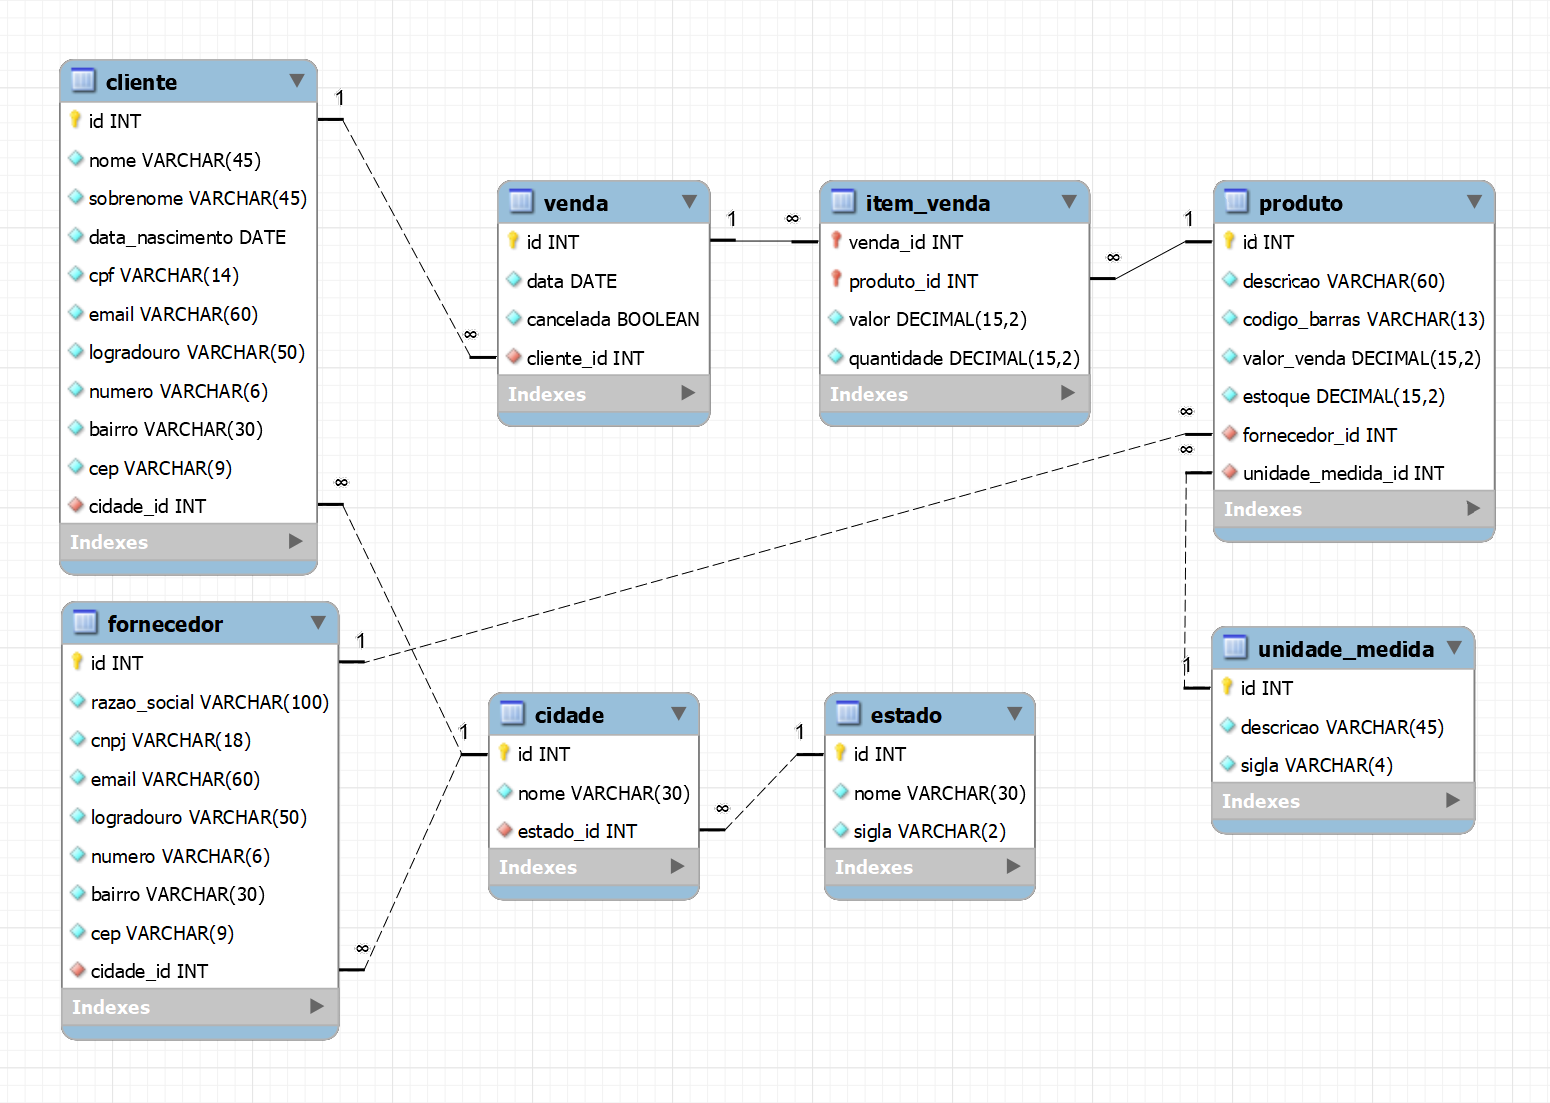
\includegraphics[scale=0.4]{imagens/cap08DER}
    \\\textbf{Fonte:} Elaborada pelo autor
    \label{fig:cap08DER}
\end{figure}
\FloatBarrier

O diagrama de classes das entidades do projeto pode ser visto Figura~\ref{fig:cap08DiagramaClasses}. Veja que a classe \texttt{ItemVenda} é a classe que fará o papel de viabilizar o relacionamento muitos-para-muitos entre produtos e vendas. Note que na UML existe a notação de classe associativa que poderia ter sido usada para representar esse relacionamento.

\FloatBarrier
\begin{figure}[!htbp]
    \centering
    \caption{Diagrama de classes das entidades}
    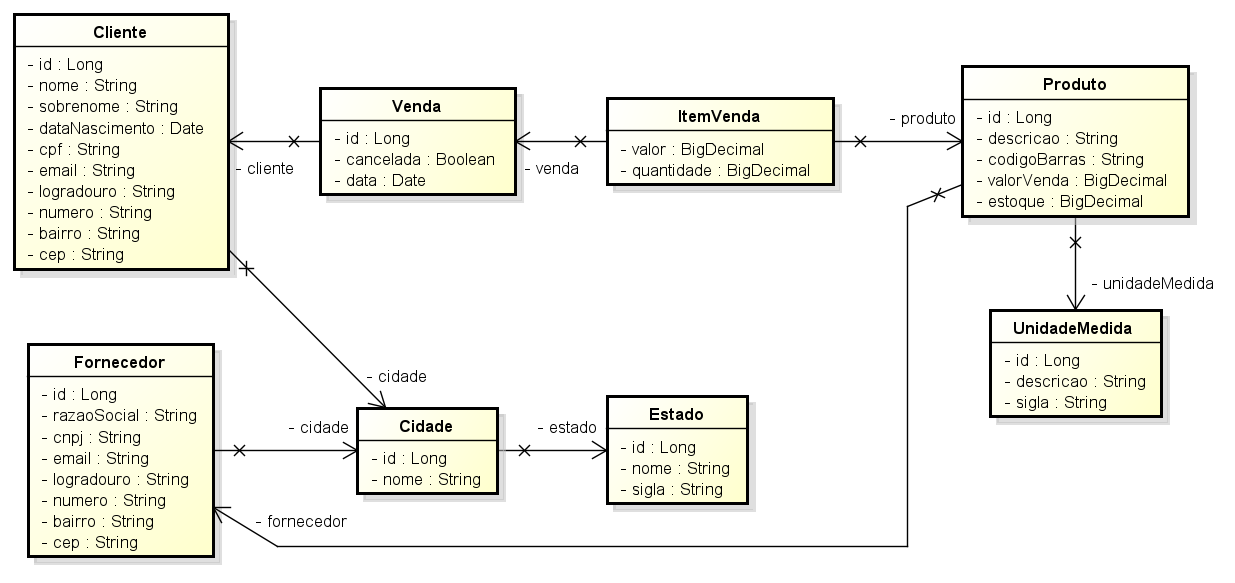
\includegraphics[scale=0.45]{imagens/cap08DiagramaClasses}
    \\\textbf{Fonte:} Elaborada pelo autor
    \label{fig:cap08DiagramaClasses}
\end{figure}
\FloatBarrier

Para que esse Capítulo não fique gigantesco, focaremos apenas nas novidades ou modificações que foram feitas em relação ao projeto anterior. Você poderá pegar o projeto pronto nos arquivos do Capítulo. A entidade \texttt{Produto} será usada como base para entendermos o que foi alterado e depois toda a parte da venda propriamente dita será detalhada com mais afinco.


\section{Construindo o Sistema}

Esta seção será dividida em várias subseções para que possamos organizar o que foi modificado em relação ao sistema anterior além, é claro, das funcionalidades novas. Os seis cadastros base são similares, então apenas um, como já explicado, será detalhado e o restante é por sua conta dar uma olhada, bastando consultar o código pronto no projeto disponibilizado.


\subsection{Entidades e Validações}

Começaremos discutindo nossas entidades. Todos os membros de todas elas agora serão de tipos de referência, ou seja, qualquer tipo que não seja primitivo. Os membros de tipo \inlineJavaCode{int}, que usamos anteriormente para definir os identificadores, passarão a ser do tipo \texttt{Long}. Todos os tipos numéricos decimais serão do tipo \texttt{BigDecimal}, principalmente quando precisarmos representar valores monetários, fugindo assim da imprecisão dos tipos de ponto flutuante, pois dinheiro é algo muito importante e precisamos tomar muito, muito, MUITO cuidado com esse tipo de dado em um sistema de verdade. Além disso, cada atributo será anotado com pelo menos uma anotação de validação, pois todos os nossos objetos das entidades serão validados, obrigatoriamente antes de serem submetidos aos seus respectivos DAOs, filtrando possíveis tentativas de adulteração dos dados submetidos através dos formulários. Na entidade \texttt{Produto}, apresentada na Listagem~\thechapter.\ref{listagem:projetos/capitulo08/VendaProdutos/src/java/vendaprodutos/entidades/Produto.java}, podemos ver isso.

\javaCode{Entidade ``Produto''\newline%
Arquivo: \texttt{vendaprodutos/entidades/Produto.java}}{projetos/capitulo08/VendaProdutos/src/java/vendaprodutos/entidades/Produto.java}

Sempre precedendo a definição de um atributo da classe utilizaremos essas anotações. Na linha 17 o atributo identificador da entidade \texttt{Produto} é declarado e, logo antes, na linha 16, é usada a anotação \inlineJavaCode{@NotNull} que indica que um objeto do tipo \texttt{Produto}, ao ser validado, não poderá ter esse atributo configurado com \inlineJavaCode{null}. Veremos o mecanismo de validação já, já. O atributo \texttt{descricao} é anotado com \inlineJavaCode{@NotNull}, que já aprendemos, e \inlineJavaCode{@Size} que, dependendo do tipo, verificará o tamanho do valor do mesmo. Para \texttt{Strings}, que é o nosso caso, é a quantidade de caracteres. Na linha 20 temos então que a descrição dos produtos pode ter no mínimo um caracetere e no máximo 60. Note que todas as nossas validações serão consistentes com as restrições existentes no DER do banco de dados. O código de barras de um produto terá obrigatoriamente que bater com um padrão de 13 dígitos, usando para isso a anotação \inlineJavaCode{@Pattern} com o atributo \texttt{regexp} (\textit{regular expression}). Essa expressão regular diz que o padrão deve casar com a String inteira, sendo que isso é indicado pelos meta-símbolos \^{} e \$ que significam, respectivamente, início e fim da \texttt{String}. O méta-símbolo \textbackslash{}d significa um dígito ($0$ a $9$) e há a necessidade de se usar duas contrabarras, pois como em Java a contrabarra indica um caracetere de escape, precisamos usar duas para escapá-la. O atributo \texttt{message} de \inlineJavaCode{@Pattern} é usado para criarmos uma mensagem personalizada para quando o produto for validado e esse atributo estiver fora do que é esperado.

A anotação \inlineJavaCode{@PositiveOrZero} indica que o atributo do tipo \texttt{BigDecimal} deve ser zero ou qualquer valor positivo. As outras anotações que usaremos nas outras entidades são \inlineJavaCode{@Positive} para valores positivos obrigatoriamente (zero não é positivo nem negativo!) e \inlineJavaCode{@Email} para verificar se o valor representa um formato válido de e-mail. A implementação de referência da \textit{Jakarta Bean Validation} faz parte do Jakarta EE 10, que estamos usando, e é fornecida pelo Hibernate Validator.

\begin{saibaMais}
    O site oficial da especificação e da implementação da API \textit{Bean Validation} pode ser acessada pelo link \url{https://beanvalidation.org/}
\end{saibaMais}

A validação dos objetos será feita sempre nos Servlets e é implementada pelo método \inlineJavaCode{validar}, que tem sua implementação iniciada na linha 187 da classe \texttt{Utils}, mostrada na Listagem~\thechapter.\ref{listagem:projetos/capitulo08/VendaProdutos/src/java/vendaprodutos/utils/Utils.java}.

\javaCode{Classe ``Utils'' com métodos estáticos utilitários\newline%
Arquivo: \texttt{vendaprodutos/utils/Utils.java}}{projetos/capitulo08/VendaProdutos/src/java/vendaprodutos/utils/Utils.java}

Na nossa implementação da validação de objetos forneceremos a opção do usuário do método ignorar a validação de atributos de uma classe, caso seja necessário. Por exemplo, um \texttt{Produto} novo não terá identificador até que seja persistido, mas precisaremos validá-lo antes de ser enviado ao seu DAO. O método validar faz uso do método estático privado \inlineJavaCode{validarObj} que é quem invoca de fato a infraestrutura de validação. Veja o código, está todo comentado. O método \inlineJavaCode{validar} lançará uma exceção do tipo \texttt{SQLException} caso o objeto seja inválido e essa exceção terá encapsulada como mensagem a descrição de todas as inconsistências identificadas no objeto. Essa mensagem será configurada com uma série de \textit{tags} \inlineHTMLCode{<li>} e será usada na página de erros da aplicação. Veremos essa questão da página de erros mais adiante no Capítulo.

Vamos ver agora o que mudou na nossa camada de persistência.


\subsection{DAO}

Temos duas novidades na nossa camada de persistência. A primeira é a implementação da interface \texttt{AutoCloseable} que permitirá que usemos objetos dos nossos DAOs na construção \textit{try-with-resources} que, por sua vez, fará o fechamento automático da conexão dos DAOs ao terminarem de serem utilizados. Para isso precisaremos implementar o método \inlineJavaCode{close} que substituirá o nosso antigo \inlineJavaCode{fecharConexao}. A implementação do DAO genérico é mostrada na Listagem~\thechapter.\ref{listagem:projetos/capitulo08/VendaProdutos/src/java/vendaprodutos/dao/DAO.java}, sendo que o método \inlineJavaCode{close} pode ser visto entre as linhas 57 e 59.

\javaCode{DAO genérico\newline%
Arquivo: \texttt{vendaprodutos/dao/DAO.java}}{projetos/capitulo08/VendaProdutos/src/java/vendaprodutos/dao/DAO.java}

A outra mudança que temos em nossos DAOs é que agora, toda entidade que tiver um objeto submetido ao método \inlineJavaCode{salvar(...)}, será modificada para conter o identificador que foi gerado pelo SGBD. Na Listagem~\thechapter.\ref{listagem:projetos/capitulo08/VendaProdutos/src/java/vendaprodutos/dao/ProdutoDAO.java} é apresentado o DAO para produtos.

\javaCode{Código da classe ``ProdutoDAO''\newline%
Arquivo: \texttt{vendaprodutos/dao/ProdutoDAO.java}}{projetos/capitulo08/VendaProdutos/src/java/vendaprodutos/dao/ProdutoDAO.java}

Veja que a criação do \texttt{PreparedStatement} do método \inlineJavaCode{salvar(...)} agora usa outra versão do método \inlineJavaCode{prepareStatement(...)} de \texttt{Connection}. Nessa versão, além da \texttt{String} contendo o código SQL que será executado, é passado um array de \texttt{Strings} com o nome da ou das colunas que representam as chaves primárias daquela tabela. Essa ``artimanha'' funciona para colunas que são auto-incrementáveis, que é o caso dos nossos identificadores. Precisaremos dessa característica no cadastro das vendas. Veremos isso mais para frente. Quando fazemos uso desse recurso, após a persistência do objeto, que gerará uma nova linha/registro/tupla na tabela, precisaremos usar o mesmo \texttt{PreparedStatement} para obter a ou as chaves. Isso será feito no método \inlineJavaCode{getChavePrimariaAposInsercao(...)} da classe \texttt{Utils} (linha 133 da Listagem~\thechapter.\ref{listagem:projetos/capitulo08/VendaProdutos/src/java/vendaprodutos/utils/Utils.java}). Como consistentemente estamos usando uma coluna chamada \texttt{id} como chave primária auto-incrementável, usaremos esse método para todas as nossas entidades, com exceção da \texttt{ItemVenda} que funcionará de outra forma. Note que o nome que foi usado é \texttt{insert\_id}, requisito necessário da versão atual do driver JDBC que estamos utilizando.

Muito bem, temos nossas entidades prontas para serem validadas e a camada de persistência atualizada. Vamos ver agora o que mudou nos nossos Servlets.


\subsection{Servlets}

Nossos Servlets continuarão a funcionar e a ter a mesma estrutura que vimos anteriormente, mas agora com algumas melhorias. Na Listagem~\thechapter.\ref{listagem:projetos/capitulo08/VendaProdutos/src/java/vendaprodutos/controladores/ProdutosServlet.java} pode ser visto o código completo do Servlet de produtos.

\javaCode{Código-fonte do Servlet ``ProdutosServlet''\newline%
Arquivo: \texttt{vendaprodutos/controladores/ProdutosServlet.java}}{projetos/capitulo08/VendaProdutos/src/java/vendaprodutos/controladores/ProdutosServlet.java}

As ações esperadas dos formulários serão as mesmas. Entre as linhas 37 e 39 instanciamos três DAOs, um para produtos, um para fornecedores e um para unidades de medida. Precisaremos dos dois últimos para trazer do banco de dados os objetos necessários para compor o produto.

A partir da linha 43 iniciam-se as instruções para obtenção dos dados do formulário de criação/inserção de um novo produto. Veja que entre as linhas 45 e 52 usamos os métodos \inlineJavaCode{getBigDecimal(...)} e \inlineJavaCode{getLong(...)} para a obtenção dos dados numéricos que virão do formulário. Estamos prevendo o caso de haver alguma inserção incorreta, passando a validação do lado do cliente e, nesses métodos, que estão definidos respectivamente nas linhas 42 e 61 da Listagem~\thechapter.\ref{listagem:projetos/capitulo08/VendaProdutos/src/java/vendaprodutos/utils/Utils.java}, é feita a obtenção dos valores e, caso haja algum problema, eles retornarão \inlineJavaCode{null} ao invés de lançar exceção. Nas linhas 54 e 55 usamos os DAOs dos fornecedores e unidades de medida para a obtenção dos objetos que contém os \texttt{ids} que vieram do formulário. Entre as linhas 57 e 63 configuramos todos os atributos do novo produto que será inserido e, na linha 65, antes de ``salvarmos'' o objeto no banco de dados, realizamos a validação. Note que estamos ignorando o atributo \texttt{id}, pois um novo produto ainda não o tem. O método de validação lançará uma \texttt{SQLException} caso haja algum erro na validação e, caso tudo esteja correto, o produto será salvo na linha 66 e na linha 67 preparamos o despacho para voltar à página de listagem. Outra coisa, após a execução do método \inlineJavaCode{salvar(...)} do DAO de produtos, o produto terá seu identificador configurado. Nesse caso não fará muita diferença, mas precisaremos desse comportamento da obtenção do \texttt{id} gerado pelo auto-incremento quando formos lidar com as vendas.

O restante dos tratamentos das ações dos formulários continuam praticamente as mesmas. Como nossos DAOs foram instanciados usando um \textit{try-with-resources}, não precisamos fechar as conexões dos DAOs de forma explícita, simplificando um pouco nosso código. Caso haja qualquer problema de validação ou mesmo em nível do SGBD, a \texttt{SQLException} lançada será capturada no \inlineJavaCode{catch} da linha 125. Ali usamos mais um método da classe \texttt{Utils}, definido na linha 218 da Listagem~\thechapter.\ref{listagem:projetos/capitulo08/VendaProdutos/src/java/vendaprodutos/utils/Utils.java}, em que preparamos o redirecionamento para a página de erros do nosso sistema. Note que na linha 223 da classe \texttt{Utils} configuramos um atributo do \textit{request} com o nome de \texttt{mensagemErro}, em que a mensagem da exceção será usada e na linha 224 configuramos o segundo parâmetro, chamado \texttt{voltarPara}, em que obtemos de qual recurso que veio a requisição para o Servlet, usando para isso o cabeçalho \texttt{Referer} da requisição, permitindo que criemos o \textit{link} apropriado para que possamos voltar à página de onde o erro foi gerado.

Por falar em erros, na Listagem~\thechapter.\ref{listagem:projetos/capitulo08/VendaProdutos/web/erro.jsp} pode ser visto o arquivo JSP que tratará os erros de validação e de persistência do sistema.

\htmlCode{Página para exibição de erros\newline%
Arquivo: \texttt{/erro.jsp}}{projetos/capitulo08/VendaProdutos/web/erro.jsp}

Com o conhecimento que você já adquiriu com o que estamos trabalhando você será capaz de entender o que essa página faz.


\subsection{Cadastro de Vendas}

Agora vamos detalhar todo o cadastro de vendas do sistema onde, de certa forma, todos os cadastros básicos convergirão. Começaremos com o lado do servidor, o chamado \textit{back-end}.

\subsubsection{\textit{Back-End}}

Na Listagem~\thechapter.\ref{listagem:projetos/capitulo08/VendaProdutos/src/java/vendaprodutos/entidades/Venda.java} pode ser vista a entidade \texttt{Venda}. Uma venda só poderá ser cadastrada e, caso necessário, ser cancelada. Estamos tentando simular um sistema real com anotações fiscais e esse tipo de coisa precisa acontecer, ou seja, uma venda nunca deve ser excluída! Para o tratamento do cancelamento temos o atributo \texttt{cancelada}.

\javaCode{Entidade ``Venda''\newline%
Arquivo: \texttt{vendaprodutos/entidades/Venda.java}}{projetos/capitulo08/VendaProdutos/src/java/vendaprodutos/entidades/Venda.java}

Na Listagem~\thechapter.\ref{listagem:projetos/capitulo08/VendaProdutos/src/java/vendaprodutos/entidades/ItemVenda.java} a entidade \texttt{ItemVenda} é apresentada. 

\javaCode{Entidade ``ItemVenda''\newline%
Arquivo: \texttt{vendaprodutos/entidades/ItemVenda.java}}{projetos/capitulo08/VendaProdutos/src/java/vendaprodutos/entidades/ItemVenda.java}

Cada venda pode conter um ou mais produtos que, por sua vez, podem ter sido vendidos em uma ou mais vendas, sendo assim, precisamos ter uma entidade que associa as outras duas. O valor do item da venda é o valor do produto naquele momento em que foi vendido, visto que o valor de venda de um produto pode variar com o tempo, mas o valor usado no momento da venda deve ser mantido! Além disso, todo item da venda tem uma quantidade associada, pois podemos ter comprado, por exemplo, duas caixas de ovos ou um quilo e meio de peito de frango.

O código do DAO que trata as vendas é apresentado na Listagem~\thechapter.\ref{listagem:projetos/capitulo08/VendaProdutos/src/java/vendaprodutos/dao/VendaDAO.java}. O método \inlineJavaCode{atualizar(...)} será usado para cancelar uma venda. Além disso, não há razão para excluirmos vendas realizadas, sendo assim, o corpo do método está vazio.

\javaCode{Código da classe ``VendaDAO''\newline%
Arquivo: \texttt{vendaprodutos/dao/VendaDAO.java}}{projetos/capitulo08/VendaProdutos/src/java/vendaprodutos/dao/VendaDAO.java}

Já o \texttt{ItemVendaDAO} é exibido na Listagem~\thechapter.\ref{listagem:projetos/capitulo08/VendaProdutos/src/java/vendaprodutos/dao/ItemVendaDAO.java}.

\javaCode{Código da classe ``ItemVendaDAO''\newline%
Arquivo: \texttt{vendaprodutos/dao/ItemVendaDAO.java}}{projetos/capitulo08/VendaProdutos/src/java/vendaprodutos/dao/ItemVendaDAO.java}

Nesse DAO temos a implementação do método \inlineJavaCode{salvar(...)}, mas a atualização, a exclusão, a obtenção de todos os itens de venda e a obtenção por \texttt{id} não são implementadas, visto que nunca mexeremos numa venda após ser feita, mas como poderemos cancelar uma venda, implementamos um método adicional no \texttt{ItemVendaDAO} chamado de \inlineJavaCode{obterPorIdVenda}, definido a partir da linha 82. Esse método retornará todos os itens de uma determinada venda para que, ao haver a necessidade de cancelá-la, possamos atualizar o estoque dos produtos, pois se uma venda foi cancelada, os produtos deverão ser devolvidos à loja e voltarão a compor o estoque.

Vamos agora fechar a implementação do nosso \textit{back-end} detalhando o Servlet das vendas. Na Listagem~\thechapter.\ref{listagem:projetos/capitulo08/VendaProdutos/src/java/vendaprodutos/controladores/VendasServlet.java} pode ser visto o código completo do mesmo.

\javaCode{Código-fonte do Servlet ``VendasServlet''\newline%
Arquivo: \texttt{vendaprodutos/controladores/VendasServlet.java}}{projetos/capitulo08/VendaProdutos/src/java/vendaprodutos/controladores/VendasServlet.java}

Esse Servlet tratará dois tipos de ação. Uma de inserção, entre as linhas 53 e 107 e uma de cancelamento, entre as linhas 108 e 130. A inserção de uma venda envolve a associação do cliente que está comprando do estabelecimento, a data da mesma e todos os itens que a compõe. Veja que a variável \texttt{itensVenda} é uma \texttt{String} que conterá dados codificados em JSON que virão do cliente. Precisaremos processar esse JSON do lado do servidor parar criar um objeto genérico que conterá o ou os identificadores do produtos e a ou as respectivas quantidades vendidas. O processo de construção desse JSON será visto quando formos tratar sobre o lado do cliente. Veremos isso logo.

Veja que o processamento do JSON dos itens da venda é feito inicialmente criando um objeto do tipo \texttt{JsonReader} nas linhas 60 e 61. Posteriormente, na linha 63 o processo de \textit{parsing} do JSON é feito, atribuindo o resultado à variável \inlineJavaCode{jsaItensVenda} do tipo \texttt{JsonArray}. Após salvarmos a venda na linha 73, iteraremos sobre \inlineJavaCode{jsaItensVenda} para extrairmos cada objeto genérico com os dados que precisamos para ``amarrar'' os produtos vendidos na venda realizada. Essa iteração ocorre entre as linhas 76 e 103, onde inicialmente obtemos o objeto genérico atual (linha 79), extraímos os dados necessários entre as linhas 82 e 85 e na linha 88 consultamos o produto e atualizamos o seu estoque (só no objeto por enquanto), visto que como estamos vendendo, precisamos subtrair a quantidade do estoque. Entre as linhas 92 e 96 criamos o item da venda, na linha 100 atualizamos o produto por causa do estoque (agora no banco de dados) e na linha 101 salvamos o item da venda. Não precisamos validar os itens de venda nem os produtos, visto que todo esse processamento será feito internamente.

O processo de cancelamento, tratado entre as linhas 108 e 130, atualizará a venda, marcando-a como cancelada e atualizará os estoques dos produtos associados. Note que não criaremos um \texttt{RequestDispatcher}, pois a ação de cancelamento será executada via AJAX. Não trataremos situações em que possam haver problemas no SGBD, pois após o cancelamento de uma venda retornaremos um JSON sinalizando que a requisição foi bem sucedida, mas em um sistema mais robusto teríamos que pensar nisso também. Uma outra coisa a se pensar, mas que não foi endereçada na nossa implementação, seria o caso de haver algum erro durante a inserção dos itens de venda ou na atualização dos produtos no cancelamento. Isso seria resolvido configurando o driver do SGBD para que as transações fossem gerenciadas manualmente e iniciadas antes das operações dos DAOs e finalizadas explicitamente com um \textit{commit} caso tudo ocorresse como esperado ou canceladas (\textit{rollback}) na detecção de algum problema.

Algo importante que não lidamos na nossa implementação é o caso de algum problema acontecer durante o processo de atualização vários tantos registros na base de dados. Imagine se o primeiro item de venda foi processado corretamente, mas no segundo, por algum motivo, aconteceu algum erro como o servidor perdeu a comunicação com o SGBD. Se isso acontecer, teremos dados corrompidos, pois o que deveria ter sido feito completamente foi feito parcialmente, concorda? Por exemplo, no caso de inserção/cadastro, o ideal seria iniciarmos uma transação antes de salvar a venda e dar um ``\textit{commit}'' nessa transação antes encaminharmos a requisição para a página de listagem, ou dar um ``\textit{rollback}'' em caso de algum problema acontecer, desfazendo o que foi feito desde o início da transação, evitando problemas na estrutura da base de dados que foi modificada. Novamente, para simplificarmos um pouco mais a implementação isso não foi endereçado. Trataremos esse tipo de situação no Capítulo de persistência, tudo bem?

Vamos agora tratar o lado do cliente.


\subsubsection{\textit{Front-End}}

Começaremos conferindo como a listagem das vendas foi implementada. Basicamente ela consiste na mesma estrutura dos outros cadastros, ou seja, uma \inlineHTMLCode{<table>} em que cada linha há um registro da tabela do banco de dados em questão. Estamos fazendo a construção dessa tabela a partir das classes de serviços, você se lembra? A novidade aqui é que uma venda não pode ser excluída ou atualizada, com a exceção de que ela pode ser cancelada. O cancelamento será feito através de uma chamada em AJAX. Para implementarmos isso, veja o \inlineHTMLCode{<c:choose>} construído entre as linhas 60 e 69 da Listagem~\thechapter.\ref{listagem:projetos/capitulo08/VendaProdutos/web/formularios/vendas/listagem.jsp}.

\htmlCode{Código da listagem de Vendas\newline%
Arquivo: \texttt{/formularios/vendas/listagem.jsp}}{projetos/capitulo08/VendaProdutos/web/formularios/vendas/listagem.jsp}

Caso uma venda esteja cancelada, a palavra ``Cancelada'' aparecerá na coluna de cancelamento. Caso contrário, entre as linhas 65 e 67, será gerado um \textit{link} apontando para ``\texttt{\#}'' no atributo \texttt{href}, sendo que o sinal ``\texttt{\#}'' sozinho indica que é uma âncora para lugar nenhum, ou seja, quando o \textit{link} for clicado, ele não fará nada. Outras \textit{tags} poderiam ter sido usadas aqui, mas para manter a consistência na GUI em relação aos outros cadastros, optei por usar \textit{hyperlinks} mesmo. Nosso \textit{link} terá mais dois atributos definidos. Um você já conhece, que é o \texttt{onclick}, apontando para a função \inlineJavaScriptCode{cancelarVenda(...)}. O outro é o atributo \texttt{data}. Esse atributo é interessante pois podemos armazenar dados nas \textit{tags}! Para usá-lo, começamos com a palavra \texttt{data}, inserimos um traço e depois um identificador qualquer, sem espaços ou letras maiúsculas. Caso queira um identificador com nome composto, ou seja, com mais de uma palavra, separe-as por traços. No nosso caso, o identificador é \texttt{id}. A ideia é que esse \textit{link} tenha um dado associado que é o identificador da venda. A função \inlineJavaScriptCode{cancelarVenda(...)} usará esse dado para saber qual venda deve ser cancelada. Note que também poderíamos ter passado o identificador da venda como argumento para a função, mas eu quis usar o atributo \texttt{data} para vocês saberem que ele existe.

\begin{saibaMais}
    Mais sobre os atributos \texttt{data}: \url{https://developer.mozilla.org/en-US/docs/Learn/HTML/Howto/Use_data_attributes}
\end{saibaMais}

Vamos dar uma olhada no arquivo de \textit{script} em que a função \inlineJavaScriptCode{cancelarVenda(...)} está implementada. Esse arquivo pode ser visto na Listagem~\thechapter.\ref{listagem:projetos/capitulo08/VendaProdutos/web/js/formularios/vendas/listagem.js}.

\javaScriptCode{\textit{Script} para cancelamento de Vendas\newline%
Arquivo: \texttt{/js/formularios/vendas/listagem.js}}{projetos/capitulo08/VendaProdutos/web/js/formularios/vendas/listagem.js}

Dentro da função temos a implementação da requisição AJAX feita tanto usando JavaScript puro, empregando a Fetch API entre as linhas 7 e 26, quanto usando jQuery, implementação essa que está comentada e é encontrada entre as linhas 29 e 46. Na linha 5 obtemos o identificador da venda através do atributo \texttt{dataset}, que é quem referencia os atributos \texttt{data} definidos no código HTML. Veja que acessamos o atributo \texttt{target} do evento, que representa quem disparou o evento, no caso o \textit{link} que foi clicado, acessamos o atributo \texttt{dataset} do \textit{link} e, por sua vez, o atributo \texttt{id} do \texttt{dataset}, que é quem está armazenando o dado que queremos, ou seja, o identificador da venda armazenado no banco de dados. Novamente, como já foi dito, poderíamos alternativamente ter passado o identificador da venda em um parâmetro dessa função.

Nossa requisição AJAX aponta para o Servlet de vendas, mapeado na URL\newline%
\texttt{/processaVendas}. Note que passamos o contexto da aplicação para a função, evitando problemas de referências quebradas. Veja que quando a requisição for feita, a ação ``cancelar'' será processada no Servlet, atualizando a coluna do registro que indica que a venda está cancelada, além de retornar ao estoque do ou dos produtos vendidos as suas respectivas quantidades. Note que em caso de sucesso, o JSON trazido do servidor será processado na linha 15 e então o objeto criado, chamado de data, será utilziado para verificar o status, que no caso só poderá ser ``ok'', e o conteúdo da célula da tabela onde a \textit{tag} \inlineHTMLCode{<a>} existia (\texttt{parentElement}) será atualizado para ``Cancelada'', não permitindo mais ser clicado, pois a partir desse momento não haverá mais um \textit{link} naquela posição.

Agora trataremos o nosso formulário de cadastro de uma nova venda. Esse formulário é um pouco mais elaborado que os anteriores, sendo que podemos ver seu código completo na Listagem~\thechapter.\ref{listagem:projetos/capitulo08/VendaProdutos/web/formularios/vendas/novo.jsp}.

\htmlCode{Formulário de cadastro de novas Vendas\newline%
Arquivo: \texttt{/formularios/vendas/novo.jsp}}{projetos/capitulo08/VendaProdutos/web/formularios/vendas/novo.jsp}

Graficamente, o código acima gerará algo como apresentado na Figura~\ref{fig:cap08FormularioNovaVenda}.

\FloatBarrier
\begin{figure}[!htbp]
    \centering
    \caption{Formulário para Novas Vendas}
    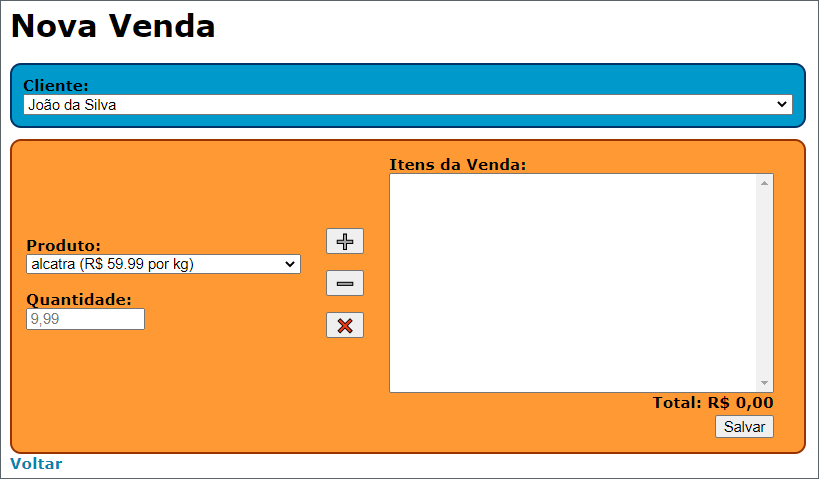
\includegraphics[scale=0.7]{imagens/cap08FormularioNovaVenda}
    \\\textbf{Fonte:} Elaborada pelo autor
    \label{fig:cap08FormularioNovaVenda}
\end{figure}
\FloatBarrier

Você já conhece praticamente todo o código utilizado na Listagem~\thechapter.\ref{listagem:projetos/capitulo08/VendaProdutos/web/formularios/vendas/novo.jsp}, sendo assim focaremos na implementação da funcionalidade apresentado na Listagem~\thechapter.\ref{listagem:projetos/capitulo08/VendaProdutos/web/js/formularios/vendas/novo.js}.

\javaScriptCode{\textit{Script} para tratamento de novas Vendas\newline%
Arquivo: \texttt{/js/formularios/vendas/novo.js}}{projetos/capitulo08/VendaProdutos/web/js/formularios/vendas/novo.js}

Neste formulário optei por fazer o registro de todos os eventos programaticamente. Na linha 6 usamos um dialeto padrão da jQuery em que registramos uma função, passada como argumento para a função \inlineJavaScriptCode{$(...)}, como ouvinte do ``evento'' \texttt{onready}. Esse evento na verdade é uma construção da biblioteca jQuery que define que quando o documento está pronto, ou seja, todo o HTML já passou pelo processo de \textit{parsing} pelo navegador, a função será executada, o que é diferente do evento \texttt{onload} da \textit{tag} \inlineHTMLCode{<body>} que é disparado quando todo o HTML e todos os recursos como imagens, arquivos externos etc. forem carregados. Note que essa função contém todas as outras que vamos usar.

Na linha 9 criamos um array que armazenará todos os itens da venda que iremos montar durante o uso do formulário. Entre as linhas 12 e 24 criamos dois formatadores de números que serão usados para formatar apropriadamente valores monetários e valores numéricos em ponto flutuante.

Entre as linhas 27 e 83 temos o evento \texttt{onclick} do botão inserir que, na Figura~\ref{fig:cap08FormularioNovaVenda}, pode ser visto entre a caixa de seleção dos produtos e a lista de itens da venda. O valor desse botão é ``\texttt{\&\#x2795;}'' que representa o emoji com sinal de mais/adição. O código em hexadecimal desse símbolo é \texttt{2795}, sendo que o prefixo \texttt{\#x} indica que é um valor em Unicode codificado em hexadecimal que deve ser processado pelo navegador e convertido em um caractere especial. Essa indicação de codificação de caractere é interpretada pelo navegador ao se iniciar tal \texttt{String} com \texttt{\&} e terminá-la com ponto e vírgula. Note que o mesmo é aplicado aos botões com o sinal de menos/subtração (botão remover) e com o símbolo de um \texttt{X} vermelho (botão limpar).

\begin{saibaMais}
    A lista completa dos emojis do Unicode pode ser vista nesse \textit{link}: \url{https://unicode.org/emoji/charts/full-emoji-list.html}
\end{saibaMais}

Para inserir um item de venda precisamos do produto e da quantidade, sendo assim obtemos os controles que detêm esses valores nas linhas 29 e 30. Entre as linhas 32 e 45 extraímos todos os dados que precisaremos para criar um objeto do item da venda. Veja que na linha 43 é criado um objeto do tipo \texttt{Decimal}. Esse tipo não é nativo do JavaScript, mas sim implementado na biblioteca \texttt{decimal.js} inserida no projeto via CDNJS. Essa biblioteca implementa tipos decimais de precisão arbitrária, assim como o tipo \texttt{BigDecimal} do Java. Como estamos lidando com quantidades de produtos do lado do cliente e não queremos arriscar ter algum tipo de erro ou problema relativo à precisão de números em ponto flutuante, vamos usar essa biblioteca. Entre as linhas 38 e 40 verificamos se o valor da venda, que é tratado como String (linha 33), contém uma vírgula separador decimal, o que provavelmente deve ser o seu caso, e caso seja, trocamos por um ponto para podermos criar um objeto do tipo Decimal quando for necessário.

Se a quantidade informada for um número maior que zero, entraremos no \inlineJavaScriptCode{if} da linha 47, ou seja, se uma quantidade válida foi informada o item da venda será criado ou a quantidade de um item existente será incrementada. Não faz sentido ter valor negativo em quantidades para o nosso problema, certo?

A primeira coisa que será feita é verificar se já existe um item de venda para o produto que está se tentando inserir na lista. Nosso banco de dados não permite que possa existir mais de um item de venda para uma mesma venda e um mesmo produto. Veja que no banco de dados a chave primária da tabela \texttt{item\_venda} é composta pelas duas chaves estrangeiras, uma de venda e uma de produto. Uma tarefa desse Capítulo será tornar isso possível. Dada essa restrição, se já houver um item de venda com o produto que se está tentando inserir, o item de venda que foi inserido posteriormente será atualizado, ou seja, sua quantidade será incrementada com a nova quantidade que se está tentando inserir. Para essa verificação, iteraremos sobre os itens da venda e, caso o identificador do produto do elemento atual for igual ao identificador do produto que se está tentando inserir na lista, a variável \inlineJavaScriptCode{itemIgual} receberá esse item e a iteração parará, por causa do retorno \inlineJavaScriptCode{true} do \textit{callback} de \inlineJavaScriptCode{some(...)}.

Na linha 59, caso o item da venda seja diferente de nulo, ou seja, foi encontrado um item da venda com o mesmo produto, atualiza-se a quantidade desse item de venda. Veja que não usamos simplesmente o operador de adição, visto que o valor do atributo quantidade é do tipo \texttt{Decimal}, havendo a necessidade de usar o método \inlineJavaScriptCode{plus} na quantidade do item, passando a quantidade a ser somada e, além disso, o retorno do método é atribuído à quantidade do item, visto que os objetos do tipo \texttt{Decimal} são imutáveis.

Se o produto que se está inserindo no novo item de venda não existe na lista, um novo item da lista será criado e inserido no array entre as linhas 68 e 73. Na linha 76 a lista de itens de venda é montada na GUI, baseando-se nos dados contidos no array \inlineJavaScriptCode{itensVenda}, além de outras atualizações na interface gráfica e na linha 77 o \textit{input} da quantidade é resetado. A linha 80 contém um alerta que será mostrado caso a quantidade fornecida na inserção seja inválida.

Entre as linhas 86 e 125 temos a implementação da remoção de itens da lista. Perceba que esta lista pode ter mais de um item selecionado ao se clicar no botão de remoção, então precisamos tratar isso. Veja na linha 108 da Listagem~\thechapter.\ref{listagem:projetos/capitulo08/VendaProdutos/web/formularios/vendas/novo.jsp} que o \inlineJavaScriptCode{<select>} de itens da venda pode ter seleção múltipla, pois contém o atributo booleano \texttt{multiple}. Essa seleção é feita na GUI mantendo pressionada a tecla \destaque{\texttt{<CTRL>}} do teclado ao se clicar nos itens.

Na linha 90 é obtido um array com todas as opções que estão selecionadas na lista. Se o tamanho desse array for zero, significa que não há itens selecionados, então uma mensagem é exibida (linha 94). Caso exista pelo menos um item, um diálogo de confirmação perguntará ao usuário se ele quer realmente remover os itens da venda selecionados. Perceba que não estamos conversando com o banco de dados! Caso o usuário escolha que os itens devem ser removidos, primeiramente precisamos iterarar pelos valores dos elementos selecionados (linha 100) e assim, para cada um desses valores, varrer o array de itens de venda (linha 103), procurando sequencialmente pelo produto e, caso encontrado, removendo esse item do array na linha 111. Ao terminar esse processo, a função \inlineJavaScriptCode{atualizarGUI()} é invocada, assim como na linha 76, para remontar a lista de itens da venda e atualizar a GUI, baseando-se no array de itens de venda.

Entre as linhas 128 e 133 temos a implementação do botão de limpar que, ao ser clicado, limpa a lista de itens de venda, ou seja, remove todos os itens de uma vez. Para isso, basta-se criar um novo array vazio para os itens da venda e, novamente, atualizar a GUI. Já falaremos dessa montagem da lista!

Entre as linhas 136 e 145 implementamos a submissão do formulário que só pode ser feita se houver pelo menos um item de venda criado. Para isso, verificamos quantos elementos do tipo \inlineHTMLCode{<option>} existem dentro do \inlineHTMLCode{<select>} de itens da venda. Se houver pelo menos um, o formulário será submetido, visto o retorno \inlineJavaScriptCode{true} na linha 143. Caso contrário, dentro do \inlineJavaScriptCode{if} de verificação dessa quantidade, será retornado o valor \inlineJavaScriptCode{false}.

Outra coisa que trataremos é remover o comportamento padrão de submissão do formulário ao se teclar \destaque{\texttt{<ENTER>}} em um campo de texto. Como temos o campo de texto das quantidades, registramos o evento \texttt{onkeydown} nele e verificamos se a tecla que foi pressionada foi o \destaque{\texttt{<ENTER>}} que tem código $13$. Se for o caso, informamos que o comportamento padrão do evento deve ser descartado, evitando a submissão do formulário.

A última coisa que precisamos conferir é a tal da função que monta os itens da venda na GUI e a atualiza. Ela está definida entre as linhas 158 e 185. Primeiramente obtém-se o componente dos itens de venda da linha 160 e na linha 161 cria-se um acumulador para armazenar o valor total da venda. Limpa-se a lista na linha 163 e itera-se sobre os itens da venda entre as linhas 165 e 180. Nessa iteração, cada item de venda é usado para criar uma nova opção para o \inlineHTMLCode{<select>} dos itens de venda. Na linha 167 calcula-se o valor do item que é composto do valor do produto multiplicado pela quantidade, entre as linhas 170 e 175 é criado um novo item da lista, na linha 177 esse item é inserido e, na linha 178, o totalizador da venda é incrementado. Ao terminar esse processo, a lista já estará atualizada com os itens que refletem o array de itens de venda, faltando atualizar o total da venda, o que acontece na linha 182 e, na linha 183, o array de itens de venda é serializado em JSON para ser enviado na submissão do formulário usando o campo escondido chamado \texttt{hiddenItensVenda}. Veja que a serialização em JSON carregará dados que não são necessários como a descrição do produto e o valor da venda. Poderíamos enviar uma forma mais enxuta desses dados mantendo um array para os dados completos e um com somente para o que é necessário para o Servlet atuar, mas deixaremos dessa forma para não complicar mais do que o necessário nesse momento.

Pronto, terminamos!


\section{Resumo}

Neste Capítulo construímos uma aplicação Web completa para a venda de produtos. Utilizamos para isso tudo que aprendemos até agora. Com isso você já é capaz de implementar a maioria dos tipos de cadastros que aparecerão em sistemas do mundo real. Parabéns! No próximo Capítulo vai ser a sua vez de desenvolver, reescrevendo e melhorando o sistema de locação de DVDs. 


\section{Projetos}

\begin{projetoSemArquivo}{}{}{}
    Modifique a implementação do projeto desenvolvido neste Capítulo para permitir que em uma venda possa existir mais de um item de venda igual. Na implementação atual isso não é permitido, pois cada registro da tabela \texttt{item\_venda} tem como chave primária a composição das duas chaves estrangeiras que a relaciona com as tabelas \texttt{produto} e \texttt{venda}. Será necessário modificar o DER e alguns detalhes da implementação do projeto, tanto do lado do servidor, quanto do lado do cliente.
\end{projetoSemArquivo}


\section{Desafios}

\begin{desafioSemArquivo}{}{}{}
    Que tal implementar a paginação das listagens dos cadastros? Imagine que numa situação real você terá centenas de produtos cadastrados, concorda? Ver todos esses produtos de uma só vez na interface gráfica pode ser um grande problema, certo? Você acabou de ser contratato em uma empresa que desenvolveu o sistema deste Capítulo e seu chefe lhe deu a tarefa de implementar a tal da paginação. Você já deve ter visto em sistemas reais, veja o destaque em laranja na Figura~\ref{fig:cap08DesafioPaginacao}. Você deve tomar todas as decisões necessárias, como quantos registros serão mostrados por página e deverá procurar como fazer esse tipo de limitação no banco de dados. Boa sorte!
    
    \FloatBarrier
    \begin{figure}[!htbp]
        \centering
        \caption{Paginação em um sistema acadêmico}
        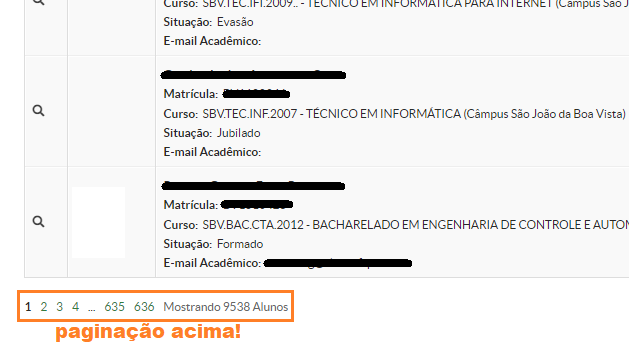
\includegraphics[scale=0.8]{imagens/cap08DesafioPaginacao}
        \\\textbf{Fonte:} Elaborada pelo autor
        \label{fig:cap08DesafioPaginacao}
    \end{figure}
    \FloatBarrier
\end{desafioSemArquivo}

\begin{desafioSemArquivo}{}{}{}
    Outra funcionalidade importante em sistemas reais é a emissão de relatórios ou de consultas personalizadas para a exibição de dados. Por exemplo, quero ter uma consulta de produtos em que eu insira parte da descrição de um produto em uma caixa de texto e, ao clicar no botão ``Consultar'', é mostrado na GUI do sistema todos os produtos que contenham na sua descrição o valor fornecido como uma substring. Pense só se o sistema tem centenas de produtos cadastrados e você precisa fazer uma venda! Imagine ficar rolando uma caixa de seleção por milhares de registro... Pois é, seu chefe gostou do seu trabalho na tarefa anterior e teu a missão de implementar essa funcionalidade no sistema. Ele quer que ao invés de ser exibida uma caixa de seleção com todos os produtos no formulário da venda, que haja um campo de texto onde o usuário fornecerá um valor que pode tanto ser o identificador do produto quanto seu código de barras e, ao teclar \destaque{\texttt{<ENTER>}} naquele campo, seja montada uma lista com os produtos obtidos, algo como mostrado na Figura~\ref{fig:cap08DesafioConsultaProduto}. Use sua imaginação e criatividade para implementar tal funcionalidade!
    
    \FloatBarrier
    \begin{figure}[!htbp]
        \centering
        \caption{Consulta de produtos no formulário de vendas}
        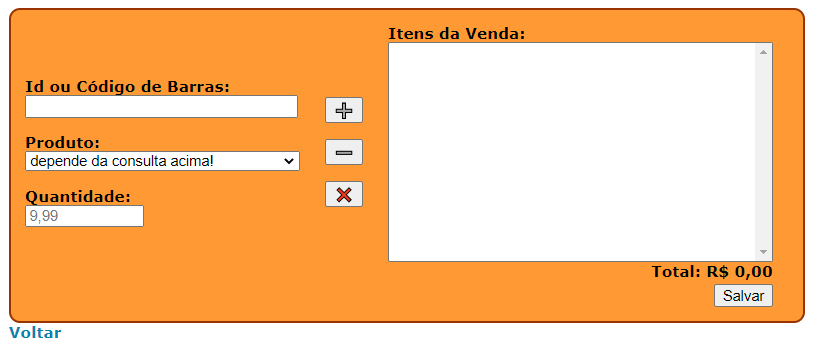
\includegraphics[scale=0.7]{imagens/cap08DesafioConsultaProduto}
        \\\textbf{Fonte:} Elaborada pelo autor
        \label{fig:cap08DesafioConsultaProduto}
    \end{figure}
    \FloatBarrier
\end{desafioSemArquivo}

\begin{desafioSemArquivo}{}{}{}
    Seu chefe adorou sua solução para o desafio anterior e agora quer mais um ``botãozinho'' no sistema. Entendedores entenderão hahaha! Ele quer que você implemente a emissão de relatórios para o sistema. Neste primeiro momento ele quer dois relatórios, um que mostre a quantidade vendida de todos os produtos em um período de tempo, ou seja, para cada produto, definindo-se uma data inicial e uma data final em um formulário, realizar a consulta no banco de dados e mostrar a quantidade que foi vendida de cada um desses produtos. O outro relatório é um relatório que mostre o montante total das vendas em um período, ou seja, ele quer saber quanto de dinheiro que entrou em um período de tempo. Você não precisa usar nada além do que já sabe, mas se quiser empregar o uso de alguma \textit{engine} de relatórios como o iReport\footnote{\url{https://community.jaspersoft.com/project/ireport-designer}}, fique à vontade. Fácil? Difícil? Seu emprego está em jogo! Mãos à obra!
\end{desafioSemArquivo}
%\chapter{Segundo Projeto: Sistema para Locação de Mídias}\label{cap:segundoProjeto}
\epigraph{``\textit{Com organização e tempo, acha-se o segredo de fazer tudo e bem feito}''.}{Pitágoras}

\lettrine[lines=4, lhang=0.1, lraise=0, loversize=0.2, findent=0.1em]{\textcolor{corTema}{N}}{ESTE} Capítulo final aplicaremos o conhecimento adquirido até o momento na construção de uma aplicação Web em Java totalmente funcional, terminando o desenvolvimento do sistema de locação de DVDs começado no Capítulo~\ref{cap:primeiroProjeto}, alterando diversas coisas que já foram feitas, inserindo a possibilidade do cadastro de mídias de vários tipos e, enfim, a locação de uma ou mais mídias por cada cliente. Sim, eu sei que locadora de DVDs, BluRays etc. não são mais tão populares, mas acredito que você saiba o que são e é um bom exemplo para podermos colocar o que sabemos em prática.


\section{Introdução}

Assim como no Capítulo~\ref{cap:primeiroProjeto}, neste Capítulo será apresentada uma série de requisitos, de forma muito simplificada, que deve ser usada para criar uma aplicação Web da mesma forma que fizemos no Capítulo~\ref{cap:sistemaVendaProdutos}. Novamente, tudo que será requisitado estará baseado no que já aprendemos, sendo assim, todas as funcionalidades requeridas poderão ser implementadas com recursos já vistos no Capítulo~\ref{cap:sistemaVendaProdutos}, mas isso não implica que você não terá que se virar de alguma forma para resolver algum problema. Agora você está apto a desenvolver um sistema completo de locação de mídias usando tudo que aprendeu até o momento. Vamos lá?


\section{Apresentação dos Requisitos}

Você foi contratado para criar um sistema para controle de cadastro de mídias. Esse sistema irá manter o cadastro dessas mídias e permitirá que clientes as aluguem. O DER do banco de dados pode ser visto na Figura~\ref{fig:cap09DER}. Para gerar a base, com o MariaDB/MySQL em execução, abra o modelo da base no MySQL Workbench, disponibilizado nos arquivos do Capítulo. Com o modelo aberto, clique no menu \destaque{\textit{Database}} escolha a opção \destaque{\textit{Forward Engineer...}} e siga o assistente. A base de dados, as tabelas e os relacionamentos serão criados, além de várias inserções em todas as tabelas, com exceção das tabelas de locação e dos itens da locação, que serão realizadas.

\FloatBarrier
\begin{figure}[!htbp]
    \centering
    \caption{DER da base de dados}
    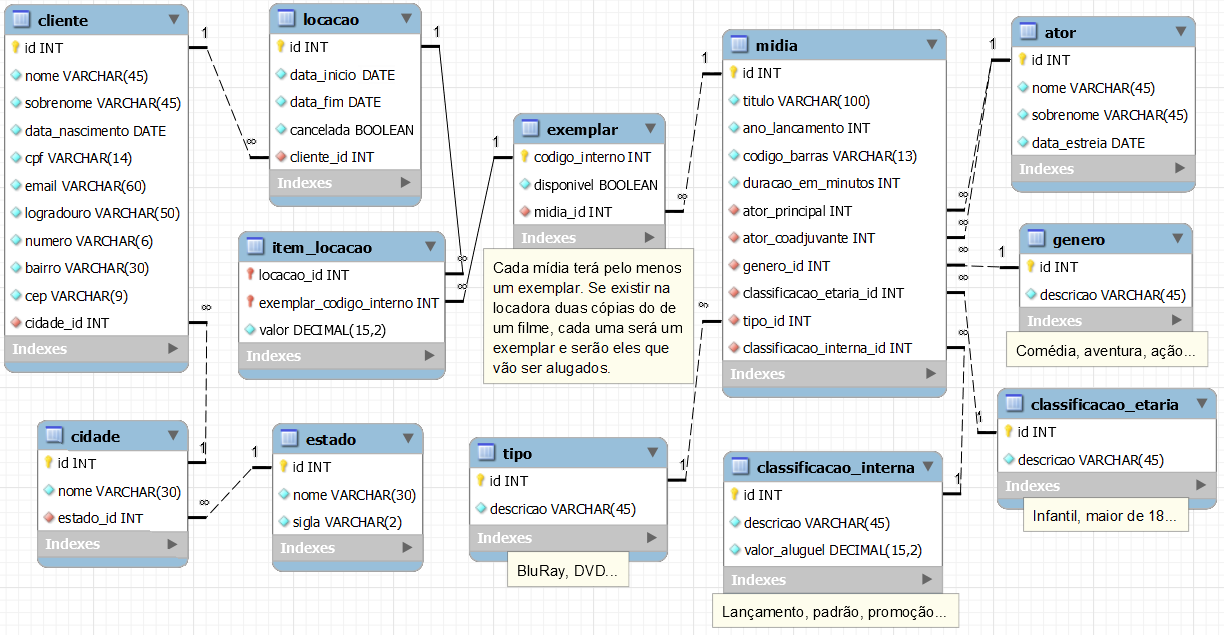
\includegraphics[scale=0.45]{imagens/cap09DER}
    \\\textbf{Fonte:} Elaborada pelo autor
    \label{fig:cap09DER}
\end{figure}
\FloatBarrier

As entidades e seus atributos você poderá ver no diagrama apresentado na Figura~\ref{fig:cap09DER}. Cada um dos cadastros base, ou seja, cadastro de mídias e seus exemplares, atores/atrizes, gêneros, classificações etárias, tipos, classificações internas, clientes, cidades e estados, deve conter as funcionalidades de criar, alterar e excluir um determinado registro. A página principal da aplicação deve conter um \textit{link} para cada tipo de cadastro. Cada mídia pode ter um ou mais exemplares. O valor da locação virá da classificação interna de uma mídia, por exemplo, quando um filme ou jogo é lançamento, a locação é mais cara, concorda? Abaixo de cada nova tabela há uma caixa de texto com alguns exemplos do que poderia haver naquele cadastro para que você possa se guiar. O processo de locação é análogo ao processo de venda de produtos do Capítulo~\ref{cap:sistemaVendaProdutos} e aqui a locação é por exemplar, então a tabela de itens de locação já está correta para a modelagem da solução desse problema, pois não será possívei alugar o mesmo examplar duas vezes na mesma locação.


\section{Desenvolvimento do Projeto}

O projeto Web que deverá ser criado deve ter o nome de ``LocacaoMidias''. Configure o projeto para conter as bibliotecas internamente. O pacote de código-fonte base do projeto deve ter o nome de ``\texttt{locacaomidias}''. A estrutura do projeto deve ser igual à estrutura do projeto criado no Capítulo~\ref{cap:sistemaVendaProdutos}, sendo que, obviamente, o nome das classes e suas respectivas implementações serão diferentes do projeto daquele Capítulo. A base de dados com as tabelas das entidades obtidas a partir da análise dos requisitos na seção anterior deve ter o nome de ``\texttt{locacao\_midias}''. Não se esqueça de que cada entidade deverá conter um identificador. As páginas da aplicação deverão ter sua aparência configurada usando uma ou mais folhas de estilos, da mesma forma que fizemos no projeto do Capítulo~\ref{cap:sistemaVendaProdutos}. Personalize os estilos, mudando as cores etc., além de usar imagens ou quaisquer outros artifícios que julgar interessante para mudar a aparência da sua aplicação. Ainda, crie um menu legal para o usuário escolher qual cadastro quer utilizar.


\section{Resumo}

Neste Capítulo foi requisitado que você implementasse uma aplicação Web em Java para gerenciar a locação de mídias como BluRays e DVDs, por isso, não há atividades a serem realizadas.


%\part{O Mundo Real}
%\chapter*{Antes de começarmos...}
\addcontentsline{toc}{chapter}{Antes de começarmos...}
\chaptermark{Antes de começarmos...}

\lettrine[lines=4, lhang=0.1, lraise=0, loversize=0.2, findent=0.1em]{\textcolor{corTema}{T}}{UDO} que vimos até agora nos serviu principalmente para criar uma base sólida de como os componentes de uma aplicação Web em Java funcionam, além de termos visto algumas coisas importantes relacionadas à linguagem JavaScript, mas apesar de ser possível criar profissionalmente aplicações Web dessa forma, talvez você tenha notado o quão demorado alguns processos são, principalmente os relacionados à persistência dos dados das entidades e a definição dos controladores da aplicação.

Nos próximos Capítulos focaremos em situações mais próximas da realidade de um desenvolvedor de aplicações Web em Java, aprendendo o essencial de vários \textit{frameworks} e bibliotecas ao aplicar o que iremos aprender na reconstrução do ``Sistema de Venda de Produtos'' do Capítulo~\ref{cap:sistemaVendaProdutos}. Nosso foco inicial será no Spring Boot, um \textit{framework} que nos ajudará a definir de forma transparente a configuração de diversos outros \textit{frameworks}, que usaremos com o objetivo de acelerar o desenvolvimento de aplicações em Java em geral que, no nosso caso, serão aplicações Web. O Spring Boot é uma baita mão na roda, pois ele cuidará de muitas coisas que teríamos que fazer manualmente, um processo tedioso e repleto de artimanhas para que as coisas funcionem da forma correta. Acredite, há alguns anos atrás, configurar diversos \textit{frameworks} e bibliotecas manualmente e, principalmente, fazer com que eles conversassem entre si era um verdadeiro pandemônio!

Agora que já sabemos mais ou menos com o que vamos lidar, nós podemos começar! Bora!!!

%\chapter{\textit{Frameworks} MVC e de Persistência}\label{cap:frameworksPersistencia}
\epigraph{``\textit{A persistência é o caminho do êxito}''.}{Charles Chaplin}

\lettrine[lines=4, lhang=0.1, lraise=0, loversize=0.2, findent=0.1em]{\textcolor{corTema}{N}}{ESTE} Capítulo reconstruiremos o ``Sistema de Venda de Produtos'' do Capítulo~\ref{cap:sistemaVendaProdutos} utilizando diversos \textit{frameworks} que tornarão nosso trabalho menos tedioso e mais direto ao ponto! A partir de agora não construiremos os nossos exemplos em sua completude, pois focaremos nas novidades e não queremos Capítulos muito extensos. Os projetos prontos estarão disponíveis como nos Capítulos anteriores.

\vfill

\section{Introdução}

Antes de começarmos a trabalhar, precisamos configurar nosso ambiente de desenvolvimento. Como lidaremos com grande parte da \textit{stack} de \textit{frameworks} e bibliotecas do Spring, poderíamos utilizar a ferramenta oficial deles para nos auxiliar, a Spring Tool Suite 4, mas não faremos isso. Eu particularmente não sou muito fã, pois ela é baseada na IDE Eclipse que, na minha opinião, é extremamente burocrática e instável, mas como ela é adotada como o padrão da indústria, uma hora ou outra acabamos ter que a adotar. Continuaremos a utilizar o NetBeans como nossa ferramenta padrão, mas você pode testar a Spring Tool Suite caso deseje. No momento em que este texto está sendo escrito, existem também versões para o Visual Studio Code (\url{https://code.visualstudio.com/}) a para a IDE Theia (\url{https://theia-ide.org/}). O \textit{download} de qualquer uma das versões pode ser feito em \url{https://spring.io/tools}.


\subsection{Criando a Primeira Aplicação Spring Boot}

A primeira coisa que vamos fazer é acessar o site Spring Initializr (\url{https://start.spring.io/}). Nesse site podermos configurar a infraestrutura básica do nosso projeto, que utilizará o Maven (\url{https://maven.apache.org/}) como ferrameta de gerenciamento do projeto. O Maven é suportado atualmente pelas principais IDEs disponíveis. Sendo um projeto Maven, espera-se que todas as IDEs trabalhem de forma semelhante, então teoriacemente podemos trabalhar com mais de uma ferramenta no mesmo projeto. Note que iremos reconstruir o ``Sistema de Venda de Produtos'' do Capítulo\ref{cap:sistemaVendaProdutos}. Vamos começar?

A versão atual da página principal do site do Spring Initializr pode ser vista na Figura~\ref{fig:cap10SpringInitializr}.

\FloatBarrier
\begin{figure}[!htbp]
    \centering
    \caption{Tela principal do site do Spring Initializr}
    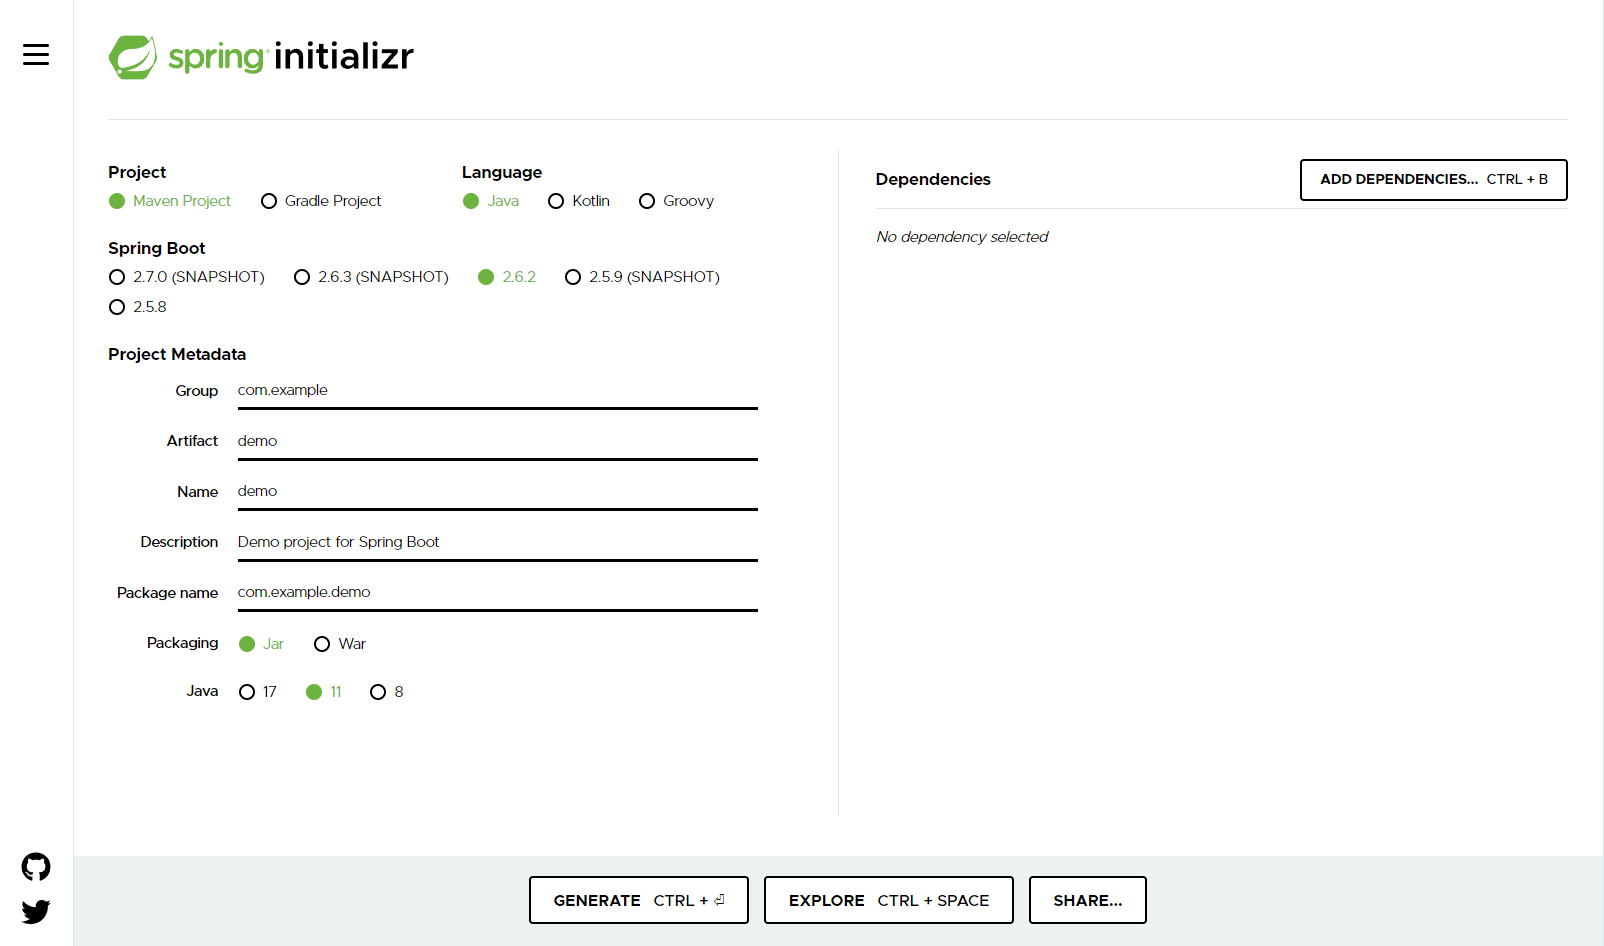
\includegraphics[scale=0.4]{imagens/cap10SpringInitializr}
    \\\textbf{Fonte:} \url{https://start.spring.io/}
    \label{fig:cap10SpringInitializr}
\end{figure}
\FloatBarrier

Basicamente, do lado esquerdo temos as opções de configuração do projeto:

\begin{itemize}

    \item \textbf{\textit{Project}:} qual ferramenta de gerencimanto de projetos que será usada (usaremos o Maven);
    
    \item \textbf{\textit{Language}:} a linguagem de programação utilizada no projeto;
    
    \item \textbf{\textit{Spring Boot}:} qual a versão do Spring Boot que usaremos;
    
    \item \textbf{\textit{Project Metadata}:} os metadados do projeto, que envolvem:
    
    \begin{itemize}
    
        \item \textbf{\textit{Group}:} nome do identificador do grupo do projeto, normalmente igual ao pacote da organização/empresa do desenvolvedor do projeto, seguindo as regras para nomeação de pacotes da linguagem Java, que por sinal podem ser acessadas usando os links apresentados na caixa ``Saiba Mais'' abaixo;
        
        \begin{saibaMais}
            \textbf{Resumo das convenções para nomeação de pacotes:}\\
            \url{https://www.oracle.com/java/technologies/javase/codeconventions-namingconventions.html}\\
            \textbf{Especificação completa sobre pacotes e módulos do Java 17:}\\
            \url{https://docs.oracle.com/javase/specs/jls/se17/html/jls-7.html}
        \end{saibaMais}
        
        \item \textbf{\textit{Artifact}:} nome do arquivo que será gerado (sem a extensão \texttt{.jar} ou \texttt{.war}) após a construção do projeto e também o identificador que será usado pelo Maven para encontrar a versão compilada e instalada do projeto dentro de seu repositório local. Normalmente se o identificador do artefato tiver mais de uma palavra, separamos as mesmas por hífens;
        
        \item \textbf{\textit{Name}:} nome do projeto, o que aparecerá na raiz do projeto aberto nas IDEs para identificá-los;
        
        \item \textbf{\textit{Description}:} breve descrição do projeto;
        
        \item \textbf{\textit{Project name}:} pacote raiz do projeto, usando como prefixo o identificador do grupo. Caso sejam usados hífens~\footnote{O Spring Initializr usará automaticamente o valor do identificador artefato aqui, trazendo hífens, que serão descartados no pacote final}, eles serão suprimidos no projeto gerado;
        
        \item \textbf{\textit{Packaging}:} tipo de empacotamento que será feito. Arquivos \texttt{.jar} podem ser executados localmente e arquivos \texttt{.war} são destinados à implantação em servidores de aplicações e/ou contêineres de Servetls. A geração de pacotes \texttt{.war} será ensinada mais adiante neste Capítulo;
        
        \item \textbf{\textit{Java}:} a versão do Java que se quer usar. Note que apenas as versões \textit{Long-Term Support} (LTS) aparecem e, além disso, você precisa ficar atento para ter um JDK de versão igual ou superior instalado na máquina de desenvolvimento e na máquina em que o projeto for executar em produção.
        
    \end{itemize}
\end{itemize}

Sabendo disso, vamos agora preparar o nosso projeto de acordo com o apresentado na Figura~\ref{fig:cap10SpringInitializrConfProjeto01}:

\FloatBarrier
\begin{figure}[!htbp]
    \centering
    \caption{Definição das propriedades do projeto}
    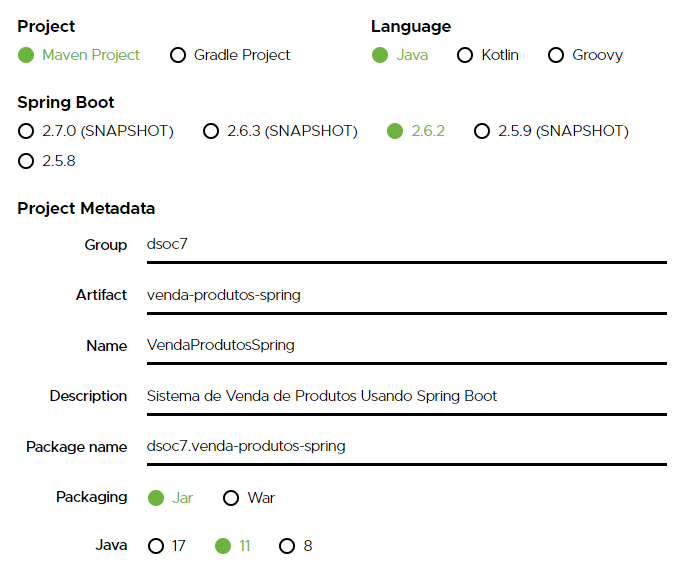
\includegraphics[scale=0.7]{imagens/cap10SpringInitializrConfProjeto01}
    \\\textbf{Fonte:} \url{https://start.spring.io/}
    \label{fig:cap10SpringInitializrConfProjeto01}
\end{figure}
\FloatBarrier

Ou seja:

\begin{itemize}

    \item \textbf{\textit{Project}:} usaremos o Maven;
    
    \item \textbf{\textit{Language}:} programaremos em Java;
    
    \item \textbf{\textit{Spring Boot}:} a última versão estável do Spring Boot, nesse caso, a \texttt{2.6.2}. Note que isso pode variar de acordo com a época que você estiver lendo esse texto. Procure usar uma versão \texttt{2.6.x} para evitarmos inconsistências, onde \texttt{x} pode ser qualquer número;
    
    \item \textbf{\textit{Project Metadata}:} os metadados do projeto, que envolvem:
    
    \begin{itemize}
    
        \item \textbf{\textit{Group}:} usaremos \texttt{dsoc7}, que é a sigla da disciplina do curso de Bacharelado em Ciência da Computação do Instituto Federal de Educação, Ciência e Tecnologia de São Paulo\footnote{Câmpus São João da Boa Vista}, para a qual esse livro foi desenvolvido incialmente, mas em um caso real, você deve preencher com a notação de domínio inverso da empresa ou instituição para a qual estiver desenvolvendo o projeto. Por exemplo, se a instuição tem o domínio \texttt{ifsp.edu.br}, você deverá preencher o identificador do grupo com \texttt{br.edu.ifsp}. Caso seja um projeto pessoal e você possuir um domínio, a regra é a mesma. Eu por exemplo tenho o domínio \texttt{davidbuzatto.com.br}, então meu identificador de grupo, para um projeto pessoal, deveria ser \texttt{br.com.davidbuzatto};
        
        \item \textbf{\textit{Artifact}:} usaremos \texttt{venda-produtos-spring};
        
        \item \textbf{\textit{Name}:} o nome preencheremos com \texttt{VendaProdutosSpring}, que é o que aparecerá no NetBeans na raiz do projeto. Aqui em um caso real você poderia usar espaços para nomear o projeto. Eu prefiro sem espaços. Note que para diferenciar do primeiro projeto de venda de produtos, adicionaremos o sufixo Spring;
        
        \item \textbf{\textit{Description}:} preencher com Sistema de Venda de Produtos Usando Spring Boot;
        
        \item \textbf{\textit{Project name}:} aqui o Spring Initializr já deve ter preenchido com a concatenção do identificador do grupo e do identificador do artefato, ficando \texttt{dsoc7.venda-produtos-spring}. Na criação do projeto esses hífens serão retirados, pois nomes de pacotes em Java não podem ter hífem;
        
        \item \textbf{\textit{Packaging}:} usaremos empacotamento em \texttt{.jar}, que é o padrão mesmo que não seja informado;
        
        \item \textbf{\textit{Java}:} usaremos o Java 11.
        
    \end{itemize}
\end{itemize}

Com isso feito, temos a configuração básica do projeto pronta, mas ainda precisamos adicionar as primeiras dependências que utilizaremos. As dependências são basicamente as bibliotecas que usaremos no projeto. A vantagem de usar um sistema de gerenciamento de projetos como o Maven é que, ao adicionarmos dependências no projeto, ele se encarregará de carregar todas as dependências que uma dependência depende, inclusive com as versões apropriadas! Nossa vida fica muito mais fácil, sem precisarmos ficar lidando com a definição de bibliotecas e isso é um super avanço na produtividade!

Para adicionar uma dependência, clique no botão \destaque{\textit{ADD DEPENDENCIES...}}. Ao fazer isso, um diálogo aparecerá, onde você poderá escolher as dependências do projeto. Ao encontrar a dependência desejada, basta clicar nela que ela será inserida na lista de dependências do projeto. Você pode procurar pelas dependências rolando a lista ou então pesquisando na caixa de texto acima. No nosso projeto utilizaremos sete dependências, apresentadas na Figura~\ref{fig:cap10SpringInitializrConfProjeto02} e descritas a seguir.

\FloatBarrier
\begin{figure}[!htbp]
    \centering
    \caption{Definição das dependências do projeto}
    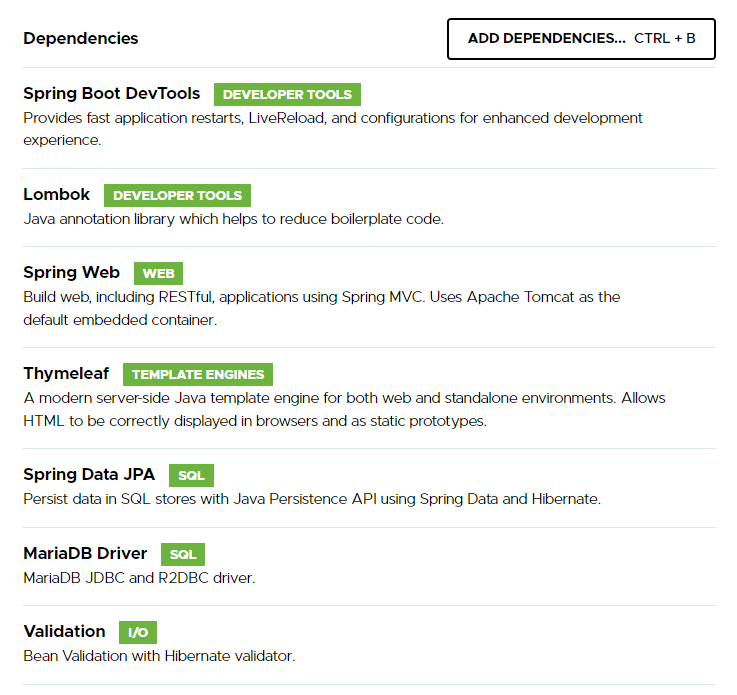
\includegraphics[scale=0.7]{imagens/cap10SpringInitializrConfProjeto02}
    \\\textbf{Fonte:} \url{https://start.spring.io/}
    \label{fig:cap10SpringInitializrConfProjeto02}
\end{figure}
\FloatBarrier

\begin{itemize}

    \item \textbf{Spring Boot DevTools:} auxília no desenvolvimento de aplicações usando Spring Boot, permitindo reinicialização rápida do servidor embarcado, integração com LiveReload etc;
    
    \item \textbf{Lombok:} é uma biblioteca de anotações que nos ajuda na criação automática de código padronizado como getters, setters, construtores etc;
    
    \item \textbf{Spring Web:} apoia a construção de aplicações Web usando o padrão de projeto MVC através do \textit{framework} Spring MVC, além da criação de Web Services RESTful;
    
    \item \textbf{Thymeleaf:} é uma \textit{template engine} que permite a definição de modelos para a criação de interfaces gráficas usando HTML, diminuindo a duplicidade de código e facilitando a manutenção;
    
    \item \textbf{Spring Data JPA:} \textit{framework} para persistência de dados usando Hibernate e a Java Persistence API (JPA);
    
    \item \textbf{MariaDB Driver:} driver de conexão com MariaDB, o SGBD que estamos utilizando neste livro;
    
    \item \textbf{Validation:} permite a validação de objetos de dados que serão gerenciados pela aplicação. Esses objetos são aqueles que estamos criando a partir das classes de modelo, nossas entidades. Podemos chamá-los também de \textit{Data Transfer Objects} (DTO), ou então de \textit{Transfer Objects} (TO). Essa validação já foi feita automaticamente nos últimos projetos, você se lembra?
    
    \begin{saibaMais}
        Se quiser saber mais sobre o Padrão de Projeto DTO/TO, dê uma olhada nesse \textit{link}: \url{https://martinfowler.com/eaaCatalog/dataTransferObject.html}.
    \end{saibaMais}
    
\end{itemize}

Agora com o inicializador do projeto configurado, clique no botão \destaque{\textit{GENERATE}}. Ao fazer isso, um arquivo \texttt{.zip} será baixado, com o nome de \texttt{venda-produtos-spring.zip}. No local onde foi salvo, descompacte-o. Abra o NetBeans e realize o procedimento de abrir projetos. Vá à pasta onde o arquivo foi descompactado. Você notará que o NetBeans reconhecerá um projeto Maven ali. Selecione-o e abra-o.

As configurações iniciais do projeto gerado no Spring Initilizr podem ser compartilhadas. Sendo assim, se você quiser, pode usar o \textit{link} abaixo para fazer o \textit{download} do projeto com as mesmas configurações apresentadas.

\url{https://start.spring.io/#!type=maven-project&language=java&platformVersion=2.6.2&packaging=jar&jvmVersion=11&groupId=dsoc7&artifactId=venda-produtos-spring&name=VendaProdutosSpring&description=Sistema%20de%20Venda%20de%20Produtos%20Usando%20Spring%20Boot&packageName=dsoc7.venda-produtos-spring&dependencies=devtools,lombok,web,thymeleaf,data-jpa,mariadb,validation}

Provavelmente, após abrir o projeto, seu NetBeans vai demorar alguns minutos --pode demorar bastante na verdade-- para baixar o índice do repositório central do Maven e prepará-lo no seu computador. Após esse processo, seu NetBeans vai ``reclamar'', informando que o repositório do Maven local não tem uma cópia das dependências do projeto. Veja na Figura~\ref{fig:cap10ConfProjeto03} o que provavelmente aparecerá, ou seja, um sinal de aviso (\textit{warning}) no ícone do projeto.

\FloatBarrier
\begin{figure}[!htbp]
    \centering
    \caption{Resolução de problema do projeto criado}
    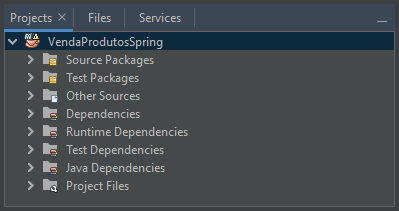
\includegraphics[scale=1]{imagens/cap10ConfProjeto03}
    \\\textbf{Fonte:} Elaborada pelo autor
    \label{fig:cap10ConfProjeto03}
\end{figure}
\FloatBarrier

Para resolvermos isso, faremos algo que talvez você já tenha feito para outras situações. Clique com o botão direito no projeto e escolha a opção \destaque{\textit{Resolve Project Problems...}} do menu de contexto. Fazendo isso, um diálogo aparecerá com um ou mais itens com o texto ``\textit{Some dependency artifacts are not in the local repository}'', indicando o problema encontrado. Clique no botão \destaque{\textit{``Resolve''}}. O Maven vai começar a realizar o processo de ``\textit{Priming}'' (preparação) do projeto, prepararando e baixando todas as dependências. Essa preparação pode demorar um pouco também. Você saberá que o processo terminou quando aparecer ``BUILD SUCESS'' na saída do NetBeans e quando o diálogo da solução dos problemas do projeto apresentar o problema apontado anteriormente com um ``check'' ou ``tick'' verde. Após esse processo, clique em \destaque{\textit{Close}}.

Agora que criamos o projeto no Spring Initializr e o abrimos no NetBeans, vamos entender sua estrutura, a qual é mostrada com seus principais nós expandidos na Figura~\ref{fig:cap10EstruturaProjeto}

\FloatBarrier
\begin{figure}[!htbp]
    \centering
    \caption{Estrutura do projeto}
    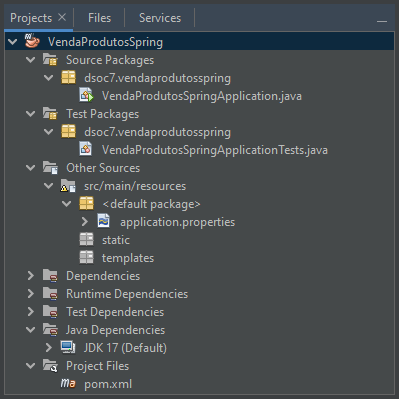
\includegraphics[scale=1]{imagens/cap10EstruturaProjeto}
    \\\textbf{Fonte:} Elaborada pelo autor
    \label{fig:cap10EstruturaProjeto}
\end{figure}
\FloatBarrier

As pastas \destaque{\textit{Source Packages}} e \destaque{\textit{Test Packages}} servirão para armazenar, respectivamente, arquivos de código fonte e arquivos de teste do projeto. A pasta \destaque{\textit{Other Sources}} será usada para armazenar quaisquer outros tipos de arquivos do nosso projeto. Note que, por padrão, o NetBeans a mostrará como as outras duas pastas, ou seja, subentendendo que é uma pasta que conterá código em Java, mas isso não é verdade. Vamos mudar a aparência de como essa pasta é exibida, deixando-a com a cara da pasta Web que estávamos acostumados nos nossos projetos anteriores, ou seja, uma exibição como uma árvore de diretórios, não de pacotes. Para isso, clique com o botão direito do mouse em \destaque{\textit{Other Sources}} e escolha a opção \destaque{\textit{Show Resources as Packages}} (Figura~\ref{fig:cap10ShowResourcesAsPackages}), desmarcando-a. 

\FloatBarrier
\begin{figure}[!htbp]
    \centering
    \caption{Estrutura do projeto}
    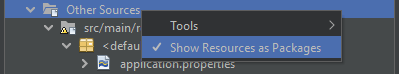
\includegraphics[scale=1]{imagens/cap10ShowResourcesAsPackages}
    \\\textbf{Fonte:} Elaborada pelo autor
    \label{fig:cap10ShowResourcesAsPackages}
\end{figure}
\FloatBarrier

Fazendo isso, a exibição dessa pasta se tornará a exibição padrão de árvore de diretórios, como mostrado na Figura\ref{fig:cap10EstruturaProjetoOK}. Dentro dela teremos inicialmente três itens: 1) O diretório \destaque{\texttt{static}} que usaremos para armazenar todos os arquivos que conterão conteúdo estático, como imagens e outros arquivos de mídia, arquivos CSS, arquivos JavaScript etc; 2) o diretório \destaque{\texttt{templates}} que conterá todos os \textit{templates} (modelos) que serão processados pelo \textit{framework} Thymeleaf e, 3) o arquivo \destaque{\texttt{application.properties}} que armazenará pares chave/valor, que serão utilizados pelo Spring Boot para alterar as configurações das dependências do projeto. Eu sei que já começaram a aparecer algumas coisas que ainda não foram explicadas, mas não se preocupe que logo veremos a serventia de cada uma delas.

\FloatBarrier
\begin{figure}[!htbp]
    \centering
    \caption{Estrutura do projeto}
    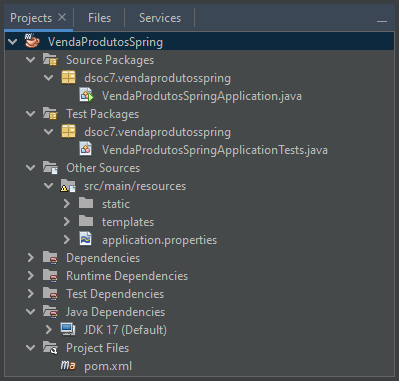
\includegraphics[scale=1]{imagens/cap10EstruturaProjetoOK}
    \\\textbf{Fonte:} Elaborada pelo autor
    \label{fig:cap10EstruturaProjetoOK}
\end{figure}
\FloatBarrier

Ainda sobre a estrutura do projeto, as pastas \destaque{\textit{Dependencies}}, \destaque{\textit{Runtime Dependencies}} e \destaque{\textit{Test Dependencies}} contém respectivamente as dependências de compilação, execução e teste do projeto. Os conteúdos delas não serão exibidos, pois contém muitos itens e eles são gerenciados diretamente pelo Maven. Na pasta \destaque{\textit{Java Dependencies}} é mostrado qual o JDK está em uso, no meu caso o 17, sendo que pode ser qualquer um com versão maior ou igual à 11 e, em \destaque{\textit{Project Files}} há um arquivo denominado \destaque{\texttt{pom.xml}} que contém as configurações do Maven para o nosso projeto. Eu não mostrarei o conteúdo aqui, pois ele estará disponível para vocês. Abra-o para dar uma olhada e siga o texto para entender o que está acontecendo em algumas de suas partes.

Entre as linhas 5 e 10 é informado que este projeto é do tipo Spring Boot, versão 2.6.2, lembrando que a versão pode variar. Entre as linhas 11 e 18 são mostrados os valores correspondentes aos metadados que preenchemos no Spring Initializr, com uma única adição, a tag \inlineHTMLCode{<version>} usada para informar a versão do projeto. Por padrão, a versão inicial vem com o conteúdo \texttt{0.0.1-SNAPSHOT}. Se você quiser mudar esse valor, fique à vontade! Agora, entre as linhas 19 e 58 são definidas todas as dependências que escolhemos no Spring Initializr. Se quisermos adicionar mais dependências, podemos editar diretamente esse arquivo ou ir no Spring Initializr, escolher a dependência que queremos inserir como gerenciada pelo Spring Boot, clicar no botão \destaque{\textit{EXPLORE}}, copiar o trecho de código XML e colar no nosso arquivo \destaque{\texttt{pom.xml}}. Dependências que não são gerenciadas pelo Spring Boot, como outras bibliotecas, também podem ser inseridas.


\subsection{Configurando e Executando a Aplicação}

Agora que já conhecemos a estrutura do projeto, poderíamos tentar executá-lo, mas como adicionamos várias dependências, nós vamos precisar configurar algumas primeiro, senão a execução não vai funcionar. Note que para colocar o projeto em execução nós \textbf{NÃO} usaremos o botão \textit{play} do NetBeans. Logo veremos como fazer. No momento vamos forçar na configuração, editando o arquivo \destaque{\texttt{application.properties}}. Abra-o e copie o conteúdo apresentado na Listagem~\thechapter.\ref{listagem:projetos/capitulo10/venda-produtos-spring/src/main/resources/application.properties}.

\propertiesCode{Primeira versão do arquivo de configuração do Spring Boot\\
Arquivo: /resources/application.properties}{projetos/capitulo10/venda-produtos-spring/src/main/resources/application.properties}

\begin{saibaMais}
    A lista completa das propriedades que podem ser configuradas no arquivo \texttt{application.properties} pode ser acessada a partir do endereço  \url{https://docs.spring.io/spring-boot/docs/current/reference/html/application-properties.html}.
\end{saibaMais}

Veja que todo o conteúdo está explicado com comentários, então não repetirei o que já foi explicado. Ainda atualizaremos esse arquivo algumas vezes durante a construção da nossa aplicação de exemplo. Vale ainda ressaltar que esse arquivo de configuração pode também ser escrito no formato YAML~\footnote{\textit{Yet Another Markup Language} \url{https://en.wikipedia.org/wiki/YAML}}. Por fim, antes de executarmos nosso projeto pela primeira vez, precisamos colocar o MariaDB no ar e criar o banco de dados com o nome de \destaque{\texttt{venda\_produtos\_spring}}. Faça isso.

Agora vamos executar nosso projeto! Logo abaixo da estrutura do projeto no NetBeans há a aba \destaque{\textit{Navigator}}. Quando o nó raiz do projeto estiver selecionado --na verdade alguns outros nós também-- serão apresentados todos os \textit{goals}/abjetivos/ações do Maven que estão disponíveis, sejam do próprio Maven ou através de \textit{plugins} definidos no arquivo \texttt{pom.xml}. Na Figura~\ref{fig:cap10PluginsMaven} essa aba é apresentada.

\FloatBarrier
\begin{figure}[!htbp]
    \centering
    \caption{\textit{Plugins} do Maven disponibilizados}
    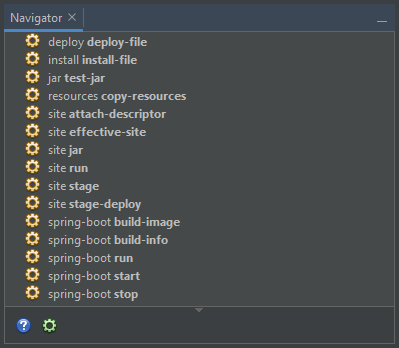
\includegraphics[scale=1]{imagens/cap10PluginsMaven}
    \\\textbf{Fonte:} Elaborada pelo autor
    \label{fig:cap10PluginsMaven}
\end{figure}
\FloatBarrier

Sendo assim, clique no nome do projeto para a aba \destaque{\textit{Navigator}} ser preenchida pelos \textit{goals} disponíveis. De todos eles, usaremos alguns. O usado para colocar o projeto no ar, compilando-o e iniciando o servidor é o \destaque{\texttt{spring-boot run}}. Clique duas vezes nele e você verá na tela de saída o Spring Boot iniciando o processo. Se tudo der certo, você terá como última linha da saída uma mensagem informando que a inicialização foi completada. Com isso, abra seu navegador (teremos que fazer isso manualmente) e acesse o endereço \url{http://localhost:8080/}. Uma página de erro será apresentada, haja vista que ainda não temos praticamente nada dentro do nosso projeto, mas com isso já sabemos que o servidor está no ar com o projeto.

Por falar em servidor, nos Capítulos anteriores tivemos que lidar com o GlassFish lembra-se? Como estamos usando o Spring MVC como dependência, o Spring Boot usará uma versão do Tomcat, que é um contêiner de Servlet como já aprendemos, embarcado no Spring MVC! Super legal não? Com isso não temos que nos preocupar com servidores durante o desenvolvimento da aplicação! Além disso, dependendo de onde a aplicação for ser implantada, poderemos executá-la igual faríamos com um \texttt{.jar} comum. Veremos isso posteriormente, além de tratarmos dos detalhes do empacotamento em arquivos \texttt{.war} para implantação em servidores remotos.

Vamos continuar, criando uma página inicial para o nosso projeto. Clique com o botão direito na pasta \destaque{\textit{templates}}, vá em \destaque{\textit{New}} e escolha \destaque{\textit{HTML File...}}. Se não houver essa opção, vá em \destaque{\textit{Other...}} e no diálogo que aparecerá, escolha a categoria \destaque{\textit{Other}}, provavelmente o último elemento da lista e do lado direito, no tipo de arquivo, \destaque{\textit{HTML File}}. Dê ok e siga o assistente, nomeando o arquivo como \destaque{\texttt{index}}. O conteúdo que seu arquivo HTML deve ter é o apresentado na Listagem~\thechapter.\ref{listagem:projetos/capitulo10/venda-produtos-spring/src/main/resources/templates/index.html}.

\htmlCode{Página inicial da aplicação\\
Arquivo: /resources/templates/index.html}{projetos/capitulo10/venda-produtos-spring/src/main/resources/templates/index.html}

Provavelmente seu projeto já está em execução, então volte ao navegador, ainda na URL \url{http://localhost:8080/} e atualize a página. Agora você verá uma página em branco com o conteúdo ``Sistema de Venda de Produtos Usando Spring Boot'' em destaque devido à \textit{tag} \inlineHTMLCode{<h1>}. Note que em comparação com o modelo usado pelo NetBeans para criar o \destaque{\texttt{index}}, a nossa versão possui algumas novidades, sendo assim, vamos explorá-las.

Perceba que a \textit{tag} \inlineHTMLCode{<html>} agora contém dois atributos. O primeiro, \inlineHTMLCode{xmlns} (XML \textit{Name Space}), indica ao navegador e também ao NetBeans --principalmente-- que nosso código HTML deve estar em conformidade com o formato \textit{EXtensible HyperText Markup Language} (XHTML), forçando que todas as nossas \textit{tags} estejam formatadas corretamente, de acordo com a versão 5 do HTML. Digo que isso é importante principalmente para o NetBeans, pois são essas duas modificações que guiarão o editor da ferramenta na acusação de erros. Para os navegadores também é importante, mas normalmente eles vão tentar se virar na hora que encontrarem erros no código HTML. O outro atributo, \inlineHTMLCode{xmlns:th}, indica que estamos criando um outro \textit{namespace}, chamado de \inlineHTMLCode{th} e associando o mesmo às \textit{tags} e atributos definidos pelo Thymeleaf. Poderia ser qualquer coisa ao invés de \inlineHTMLCode{th}, mas seguiremos o padrão. Veja que um paralelo que podemos fazer com algo que já vimos seria com as \textit{tags} da JSTL. Esse tal de Thymeleaf já apareceu algumas vezes no texto e ele logo será explicado, fique tranquilo! Note que agora precisamos obrigatoriamente terminar a \textit{tag} \inlineHTMLCode{<meta>} com uma barra, o que não era necessário se não houvesse essa restrição de conformidade ao XHTML.

Vamos fazer mais um teste para ver o que acontece. Acesse a URL \url{http://localhost:8080/index} ou \url{http://localhost:8080/index.html}. O que aconteceu? Erro novamente! Aí você se pergunta: ``Afinal, eu já não tenho o arquivo do index no projeto? Porque a URL não `funciona'?''. A resposta está em como o Spring MVC funciona. Todo e qualquer recurso que fará parte da camada \textit{View} precisa de alguma forma ser ``registrado'', associando um caminho relativo, que será exposto como URL, e o recurso em si. Automaticamente, a raiz do contexto é associada a um arquivo chamado \texttt{index.html}, mas se quisermos acessar esse arquivo de outra forma, precisamos dizer isso ao Spring MVC. Quando formos implementar nossos controladores e ao utilizar o Thymeleaf, esses registros serão feitos programaticamente, seja nas classes dos controladores, por meio de anotações, ou no código dos \textit{templates}, mas se quisermos que outro recurso seja exposto, precisamos informar isso ao \textit{framework}. Vamos fazer isso? Note que o que vamos fazer é totalmente opcional no nosso caso, mas faremos para termos como exemplo e caso você precise realizar tal operação.


\subsection{Realizando Configurações Programaticamente}

A primeira coisa que faremos é criar um novo pacote, chamado de \destaque{\texttt{web}}, dentro do pacote \destaque{\texttt{dsoc7.vendaprodutosspring}}. Cuidado, estamos trabalhando nos pacotes de código fonte, não nos pacotes de teste! Outra coisa importante. Todo e qualquer código que será gerenciado pelo Spring Boot, pelo Spring Framework e pelo Spring MVC precisa estar, obrigatoriamente, dentro do pacote principal do projeto, no nosso caso o \destaque{\texttt{dsoc7.vendaprodutosspring}}, que contém a classe \destaque{\texttt{VendaProdutosSpringApplication}}, ou em algum de seus subpacotes.

No pacote \destaque{\texttt{dsoc7.vendaprodutosspring.web}} recém criado, crie uma classe chamada de \inlineJavaCode{WebConfig}. O nome poderia ser qualquer coisa, mas vamos chamar assim para darmos a noção que essa classe fará a configuração da parte ``web'' do Spring MVC. Veja o código da classe na Listagem~\thechapter.\ref{listagem:projetos/capitulo10/venda-produtos-spring/src/main/java/dsoc7/vendaprodutosspring/web/WebConfig.java}.

\javaCode{Classe de configuração\\
Arquivo: /dsoc7/vendaprodutosspring/web/WebConfig.java}{projetos/capitulo10/venda-produtos-spring/src/main/java/dsoc7/vendaprodutosspring/web/WebConfig.java}

Na linha 12 usamos uma anotação \inlineJavaCode{@Configuration} do Spring Framework, que informa ao Spring que essa classe é uma classe de configuração, ou seja, ela executará tarefas de configuração da aplicação. Essa classe implementa a interface \inlineJavaCode{WebMcvConfigurer}, que define vários métodos para configurar programaticamente o Spring MVC. O método que vamos implementar no momento é o \inlineJavaCode{addViewControllers}, que pelo nome podemos perceber que irá realizar a adição de controladores de visualizações na nossa aplicação. Esse método tem como parâmetro um \inlineJavaCode{ViewControllerRegistry} que é o tal do registro que associa um caminho à um recurso --normalmente uma \textit{view}-- e que será usado pelo Spring MVC para chegar até o recurso desejado pela URL requisitada. Esse mapeamento é muitas vezes também chamado de rota. No nosso exemplo, adicionamos dois caminhos ao recurso \destaque{\texttt{index}}. Na linha 18, o primeiro caminho, \destaque{\texttt{/index}}, é associado ao recurso \destaque{\texttt{index}} e o caminho \destaque{\texttt{/index.html}} é associado ao mesmo recurso. Note que o caminho parte da raiz da aplicação e que o recurso está contido na pasta \destaque{\texttt{templates}} do projeto. Salve sua classe se ainda não o fez e vá no navegador testar as duas URLs que não estavam funcionando. O que aconteceu? Agora sim não é?


\subsection{O Ponto de Entrada de Uma Aplicação Spring Boot}

Vamos continuar a explorar essa fase inicial de preparação e de entendimento do nosso projeto? Uma aplicação Spring Boot pode ser tanto Web como Desktop. A nossa é Web, óbvio. Enquanto em aplicações Web ``tradicionais'' não existe muito bem definido um ponto de entrada da execução da aplicação (um ``método \texttt{main}''), pois isso fica escondido atrás dos servidores de aplicação e dos dos contêineres de Servlets, numa aplicação Spring Boot isso é definido. Veja que dentro do pacote \destaque{\texttt{dsoc7.vendaprodutosspring}} há uma classe, que já mencionamos a alguns parágrafos, chamada de \inlineJavaCode{VendaProdutosSpringApplication}, criada automaticamente pelo Spring Initializr. O código da mesma pode ser visto na Listagem~\thechapter.\ref{listagem:projetos/capitulo10/venda-produtos-spring/src/main/java/dsoc7/vendaprodutosspring/VendaProdutosSpringApplication.java}.

\javaCode{Classe de definição de aplicação Spring Boot\\
Arquivo: /dsoc7/vendaprodutosspring/VendaProdutosSpringApplication.java}{projetos/capitulo10/venda-produtos-spring/src/main/java/dsoc7/vendaprodutosspring/VendaProdutosSpringApplication.java}

Essa classe está anotada com \inlineJavaCode{@SpringBootApplication}, que é uma anotação do Spring Boot e que indica que essa classe é uma aplicação Spring Boot. Essa classe deve ter um método \texttt{main}, normalmente com uma linha de código e, apesar de poder haver configurações implementadas nela, deixaremos isso para as classes de configuração como a \inlineJavaCode{WebConfig} que criamos há pouco. Na linha de código presente dentro do método \texttt{main} o método estático \texttt{run} da classe \inlineJavaCode{SpringApplication} é executado, passando-se uma referência ao tipo da classe \inlineJavaCode{VendaProdutosSpringApplication} e os argumentos que porventura foram fornecidos ao método \texttt{main}. Não precisaremos mexer com ela se formos trabalhar com empacotamento em \texttt{.jar}, mas se mudarmos para \texttt{.war} precisaremos fazer algumas modificações. Isso fica para depois, como já falei.


\subsection{Atualizações Automáticas do Navegador Usando LiveReload}

Estamos quase terminando essa parte introdutória! Vamos tratar agora sobre outra funcionalidade que nos ajuda na produtividade. Toda vez que alteramos algo no projeto, já sabemos que o Spring Boot DevTools vai atualizar os arquivos do projeto no Tomcat que está em execução, bastando irmos no navegador e atualizar a página para testarmos o que acabamos de fazer. Isso já nos poupa de mandar o projeto rodar de novo em algumas situações. Agora vamos ver o que podemos fazer para a atualização da página ser automática, ou seja, ao alterarmos algo no projeto e salvarmos, a página já estará atualizada ou em processo de atualização no navegador.

Para isso, precisamos instalar uma extensão no Chrome (\url{http://livereload.com/}), chamada de \destaque{LiveReload}. Há versões para outros navegadores também, mas detalharei a versão do Chrome, pois é o navegador que eu uso e que provavelmente a maioria de vocês também. Para a instalação no Chrome, entre na seção de extensões da Chrome Web Store (\url{https://chrome.google.com/webstore/category/extensions}) e na caixa de pesquisa, procure por LiveReload. Pode ser que haja mais de um resultado. A que estamos procurando é a ``oferecida por \url{http://livereload.com/}'' e versão atual é a 2.1.0, mas isso, como você já sabe, pode variar de acordo com a época que você está lendo este livro. Clique nela e depois no botão \destaque{Usar no Chrome}. Isso fará com que um botão\footnote{Algo parecido com isso 
\includegraphics[scale=1]{imagens/cap10BotaoLiveReloadBranco}, ou isso 
\includegraphics[scale=1]{imagens/cap10BotaoLiveReloadPreto}.} seja adicionado na barra de endereços do Chrome. Ao clicar nele uma vez, o LiveReload será ativado. A partir de agora, toda alteração que for feita em arquivos HTML, CSS, JavaScript etc, disparará uma atualização automática na página que está atualmente sendo mostrada, visto que o DevTools enviará, via WebSocket, uma notificação ao LiveReload. Faça um teste. Mude algo no \texttt{index.html}, salve e volte ao navegador. A alteração ou já estará sendo exibida ou a página estará sendo atualizada. Se ainda não estiver funcionando matando o \textit{goal} \destaque{\texttt{spring-boot run}} que ainda está em execução clicando no \texttt{x} do indicador de processos do NetBeans\footnote{Canto inferior direito, algo parecido com isso 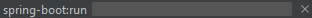
\includegraphics[scale=1]{imagens/cap10MatarProcessoSpringBootRun}}, a inicie novamente com o \textit{goal} \destaque{\texttt{spring-boot run}}, atualize a página no Chrome, faça a alteração no código HTML do \texttt{index.html} e veja a atualização ser feita automaticamente a partir de agora. Deve funcionar.

Muito bem! Temos a infraestrutura básica do nosso projeto pronta para podermos começar a trabalhar de verdade! Iremos agora começar a construir novamente, camada por camada, nossa aplicação de Venda de Produtos, mas agora usando diversas bibliotecas, \textit{frameworks} e recursos que, graças ao Spring Boot, já estão prontos para serem utilizados. Para não ficar muito extenso e cansativo, irei focar em algumas entidades para você aprender o que quero ensinar. O código completo do projeto estará disponível para consulta, como de praxe. Vamos lá!

\begin{saibaMais}
    As documentações das versões atuais do Spring Boot podem ser acessadas no endereço \url{https://spring.io/projects/spring-boot#learn}
\end{saibaMais}

\section{JPA, Hibernate, Validações e Lombok}

Agora vamos começar a definir nossas entidades começando com a \inlineJavaCode{Estado}. Teremos várias novidades na nossa classe e vamos tratar todas elas. Primeiramente, crie o pacote \inlineJavaCode{entidades} dentro do pacote \inlineJavaCode{dsoc7.vendaprodutosspring} do projeto e dentro dele crie uma classe chamada \inlineJavaCode{Estado}. Na Listagem~\thechapter.\ref{listagem:projetos/capitulo10/venda-produtos-spring/src/main/java/dsoc7/vendaprodutosspring/entidades/Estado.java} podermos ver o código de tal classe.

\javaCode{Entidade Estado\\
Arquivo: /dsoc7/vendaprodutosspring/entidades/Estado.java}{projetos/capitulo10/venda-produtos-spring/src/main/java/dsoc7/vendaprodutosspring/entidades/Estado.java}

A primeira novidade que temos é na linha 20 o uso da anotação \inlineJavaCode{@Entity}. Essa anotação faz parte da \textit{Java Persistence API} (JPA) que é uma API que trata de persistência, ou seja, da ``transferência'' de objetos do lado da linguagem Java para suas respectivas representações no modelo relacional e vice-versa, instanciadas em um SGBD específico. Esse processo de comunicação entre os mundos Orientado a Objetos e Relacional é chamado de Mapeamento Objeto-Relacional ou \textit{Object-Relational Mapping} (ORM) e é realizado por \textit{frameworks} ORM. Antes da criação da JPA, esses \textit{frameworks} precisavam ser configurados manualmente, normalmente através de arquivos XML, o que era bastante burocrático e despadronizado. A ideia da JPA foi padronizar o processo de ORM, definindo uma série de especificações que os \textit{frameworks} deveriam implementar. O Hibernate é um desses \textit{frameworks} e é ele que possui a maioria, senão todas, as implementações de referência da JPA e de especifgicações correlatas. Voltando ao código...

A anotação \inlineJavaCode{@Entity} indica à unidade de persistência --\textit{persistence unit}-- que os objetos dessa classe/entidade são objetos que passarão pelo processo de ORM. Como estamos usando o Spring Boot a criação da unidade de persistência será feita automaticamente por ele. Em um projeto sem o Spring Boot, teríamos que configurar a unidade de persistência manualmente em um arquivo de configuração chamado de \texttt{persistence.xml}. A partir do momento que anotamos a classe com \inlineJavaCode{@Entity}, podemos configurar seus atributos usando várias anotações da JPA e da API \textit{Bean Validation}, que já vimos, indicando as características que esses atributos terão no SGBD que será utilizado. Outra coisa importante é que os \textit{frameworks} ORM, no nosso caso o Hibernate, precisam saber qual SGBD está sendo utilizado para que todo o SQL que será gerado automaticamente seja escrito na sintaxe correta do SGBD em questão. Isso, novamente, será tratado automaticamente pelo Spring Boot quando definirmos a dependência de SGBD que vamos utilizar. Lembre-se que na criação do projeto no Spring Initalizr definimos que queríamos o driver do MariaDB e, ao adicionar aquela dependência, o Spring Boot já vai saber como configurar o Hibernate para o MariaDB. O que eu quero que você entenda com tanta explicação é que, sem o Spring Boot, teríamos que fazer tudo isso manualmente, enchendo nosso projeto de arquivos de configuração. Acredite, isso dá muito mais trabalho.

Veja, agora que usaremos a JPA e o Hibernate, não precisaremos mais escrever código padronizado para operações básicas no SGBD, ou seja, podemos dar tchau para os nossos antigos DAOs! Chiquérrimo não? Um problema a menos na nossa vida.

Assim que anotarmos a classe com a anotação \inlineJavaCode{@Entity}, o NetBeans vai reclamar que o projeto não tem a unidade de persistência que já informei. Você não precisa fazer nada, pois o Spring Boot vai dar conta disso. O NetBeans não entende que para um projeto usando Spring Boot ele não precisa reclamar.

Todo esse processo de criar objetos que serão usados, seja baseado em configurações que precisariam ser feitas manualmente ou então que dependem de outros recursos será gerenciado pelo Spring Framework (não é o Boot) de forma automática atravás da Inversão de Controle --\textit{Inversion of Control} (IOC)-- e de sua ``versão'' mais especializada chamada de Injeção de Dependência --\textit{Dependency Injection} (DI)-- pois, afinal de contas, o objetivo principal do Spring Framework é justamente esse. Logo veremos alguns exemplos disso na nossa implementação. Vamos continuar agora com o código da Listagem~\thechapter.\ref{listagem:projetos/capitulo10/venda-produtos-spring/src/main/java/dsoc7/vendaprodutosspring/entidades/Estado.java}.

Por enquanto, vamos pulhar as anotações usadas entre as linhas 21 e 24, mas daqui um pouco voltaremos nossa atenção à elas. Vamos tratar primeiros das anotações de persistência e validação. A classe \inlineJavaCode{Estado} possui três atributos. Um identificador do tipo \inlineJavaCode{Long}, um nome do tipo \inlineJavaCode{String} e uma sigla do tipo \inlineJavaCode{String}. Em relação ao identificador, chamado de \inlineJavaCode{id} e definido na linha 30, usamos a anotação \inlineJavaCode{@Id} na linha 27 para indicar que esse atributo faz parte de chave primária da tabela que representará a entidade \inlineJavaCode{Estado} e na linha 28 usamos a anotação \inlineJavaCode{@GeneratedValue} para indicar que o valor do identificador será gerado pelo SGBD como um auto-incrementável por causa da estratégia configurada como \inlineJavaCode{GenerationType.IDENTITY}. A anotação da linha 29 nós vamos pular, já já voltamos nela. Perceba que não usamos a anotação \inlineJavaCode{@NotNull} no identificador, pois afinal, ele será gerado automaticamente quando criarmos um novo objeto do tipo \inlineJavaCode{Estado} e o persistirmos no SGBD. Se usarmos essa anotação, ao criarmos um novo objeto do tipo \inlineJavaCode{Estado} e esse objeto for validado antes de ser persistido, o que vai acontecer de fato, esse objeto será tratado como inválido e não é isso que queremos. O atributo nome, linha 36, está anotado com as anotações \inlineJavaCode{@NotNull} e \inlineJavaCode{@Size}, linhas 32 e 33 respectivamente, que já conhecemos. Essas anotações, além de serer anotações de validação, também serão utilizadas como base para configurar os atributos/colunas da tabela no SGBD, ou seja, o atributo nome da tabela será \inlineSQLCode{NOT NULL} por causa da anotação \inlineJavaCode{@NotNull} e o tipo \inlineSQLCode{VARCHAR}, que virá do tipo \inlineJavaCode{String} do atributo da classe, terá aplicado a restrição de tamanho informada na anotação \inlineJavaCode{@Size}. Veja que o atributo sigla, definido na linha 43, está anotado também com \inlineJavaCode{@NotNull} e \inlineJavaCode{@Size}, além de ter a anotação \inlineJavaCode{@Column}, que é usada para passar configurações extras para o framework de ORM. Nesse caso, informamos que a coluna que representará a sigla do estado tem valor único (UNIQUE CONSTRAINT). Logo veremos que a grande sacada de tudo isso é que poderemos focar somente no mundo Orientado a Objetos e deixar o lado relacional para o Hibernate. Isso deixa o pessoal que gosta de Banco de Dados de cabelo em pé, mas o que importa é sermos produtivos! A partir dessas configurações feitas através dessas anotações, quando rodarmos o projeto e tivermos tudo confirado apropriadamente, o Hibernate gerará o código da \textit{Data Definition Language} (DDL) para criar a tabela estado. Nesse caso, teremos algo como apresentado na Listagem~\thechapter.\ref{listagem:projetos/capitulo10/parciais/estado.sql}.

\sqlCode{DDL da tabela estado gerada automaticamente pelo Hibernate a partir das anotações na entidade Estado}{projetos/capitulo10/parciais/estado.sql}

Agora vamos tratar das anotações que faltaram. Não sei se você percebeu, mas no código da classe \inlineJavaCode{Estado} ficou faltando a definição do construtor e dos métodos \textit{get} e \textit{set} dos atributos não é mesmo? E se eu te contar que vamos poder gerar isso automaticamente também, sem nem mesmo precisar mexer no código? É justamente disso do que se trata as outras anotações. No nosso projeto incluímos como dependência a bilioteca Lombok. Essa biblioteca contém uma série de anotações que ``interagem'' com o compilador Java e insere código padrão como \textit{getters}, \textit{setters}, construtores, implementação (correta!) dos métodos \inlineJavaCode{equals}, \inlineJavaCode{hashCode} e outras coisas mais. O NetBeans e as outras IDEs famosas reconhecem o Lombok e vão entender que uma classe anotada com as anotações da biblioteca terá, depois de compilada, as ``coisas'' que foram definidas para serem criadas, não reclamando que o código não existe nos arquivos e até sugeringo o uso dos métodos nas ferramentas de auto-completar. Voltamos então à Listagem~\thechapter.\ref{listagem:projetos/capitulo10/venda-produtos-spring/src/main/java/dsoc7/vendaprodutosspring/entidades/Estado.java}. A anotação \inlineJavaCode{@Data} é a principal anotação do Lombok e foi inserida na linha 21. A partir do uso dessa anotação, a biblioteca já fará muita coisa automaticamente, como criar os \textit{gets}, os \textit{sets}, os métodos \inlineJavaCode{equals} e \inlineJavaCode{hashCode}. A partir dai, podemos mandar ela fazer mais ou menos coisas para nós. No nosso caso, pedimos para que o construtor que recebe como parâmetro todos os atributos da classe seja criado, ao usar a anotação \inlineJavaCode{@AllArgsConstructor} na linha 22 e que o construtor padrão, aquele que não recebe nenhum parâmetro, também seja criado ao usar a anotação \inlineJavaCode{@NoArgsConstructor} na linha 23. Por padrão, os métodos \inlineJavaCode{equals} e \inlineJavaCode{hashCode} gerados pelo Lombok utilizarão todos os atributos da classe, mas no nosso caso, somente o identificador é necessário, visto que lá no mundo relacional, é ele que é a chave primária e que garante a unicidade de tupla. Sendo assim, na linha 24 usamos a anotação \inlineJavaCode{@EqualsAndHashCode} com a propriedade \inlineJavaCode{onlyExplicitlyIncluded} configurada como \inlineJavaCode{true} para indicar ao Lombok que nós queremos dizer explicitamente a ele qual ou quais atributos serão utilizados nos métodos \inlineJavaCode{equals} e \inlineJavaCode{hashCode}. Como já informei, para o nosso caso apenas o identificador faz sentido --por causa da tabela-- e então anotamos ele com a anotação \inlineJavaCode{@EqualsAndHashCode.Include}. Faz sentido né?

Agora que já sabemos tudo o que está acontecendo na nossa classe \inlineJavaCode{Estado}, podemos testar para ver se o Hibernate está gerando a tabela apropriadamente, se conseguimos realizar as operações CRUD nela e, além disso, veremos como configurar um \textit{script} SQL para realizar a carga inicial das tabelas do banco de dados da aplicação para nós.

criar repositório
criar teste
carga inicial no banco através do import.sql
por figura mostrando o pacote da classe estado

\section{Spring MVC}

criação dos controladores e páginas com thymeleaf

importância das diretivas de pré-processamento, de busca de propriedades, de resolução de contexto etc.

\begin{comment}
    @{}, ${}, *{}, __${}__, T(classe).métodoEstático, tags th, blocos sintáticos
\end{comment}


\subsection{Outros \textit{Frameworks} MVC}

%Falar brevemente de: JavaServer Faces (JSF), Struts, VRaptor etc.

\section{Execução Local do Projeto}

falar do .jar


\section{Resumo}

\section{Exercícios}

\section{Projetos}

%\chapter{\textit{Web Services RESTful}}\label{cap:webservicesRestful}
\epigraph{``\textit{Não extingua sua inspiração e sua imaginação; não se torne o escravo do seu modelo}''.}{Vincent van Gogh}

\lettrine[lines=4, lhang=0.1, lraise=0, loversize=0.2, findent=0.1em]{\textcolor{corTema}{N}}{ESTE} Capítulo aaa.

\vfill

\section{Introdução}

criação de controladores rest e consumir API usando Javascript.

talvez uma inserção e uma listagem?

atualização do CORS via configuração programática (funciona só no .jar)
/*@Override
    public void addCorsMappings( CorsRegistry registry ) {
        registry.addMapping( "/**" )
                .allowedMethods( "*" );
                //.allowedMethods( "HEAD", "GET", "PUT", "POST", "DELETE", "PATCH" );
    }*/

\section{Resumo}

\section{Exercícios}

\section{Projetos}

%\chapter{\textit{Frameworks} e Bibliotecas \textit{Front-End}}\label{cap:frameworksBibliotecasFront}
\epigraph{``\textit{A beleza interessa nos primeiros quinze dias; e morre, em seguida, num insuportável tédio visual}''.}{Nelson Rodrigues}

\lettrine[lines=4, lhang=0.1, lraise=0, loversize=0.2, findent=0.1em]{\textcolor{corTema}{N}}{ESTE} Capítulo serão tratados os conceitos básicos dos principais \textit{frameworks} da camada de visualização que podem ser aplicados para construção de aplicações Web em Java.

\vfill

\section{Introdução}

\section{Bootstrap}

\section{jQuery UI}

\section{AngularJS}

\section{Outros}

%Falar brevemente de: ExtJS, Vue.js, React etc.

\section{Resumo}

\section{Exercícios}

\section{Projetos}

%\chapter{Terceiro Projeto: }\label{cap:terceiroProjeto}
\epigraph{``\textit{O futuro não é um lugar onde estamos indo, mas um lugar que estamos criando. O caminho para ele não é encontrado, mas construído e o ato de fazê-lo muda tanto o realizador quando o destino}''.}{Antoine de Saint-Exupéry}

\lettrine[lines=4, lhang=0.1, lraise=0, loversize=0.2, findent=0.1em]{\textcolor{corTema}{N}}{ESTE} Capítulo aaa.

\vfill

\section{Introdução}



\section{Resumo}

Neste Capítulo foi requisitado que você implementasse uma aplicação ...

%\chapter{Empacotamento em Web Archive (\texttt{.war}) e Implantação}\label{cap:empacotamento}
\epigraph{``\textit{Information about the package is as important as the package itself}''.}{Frederick W. Smith}

\lettrine[lines=4, lhang=0.1, lraise=0, loversize=0.2, findent=0.1em]{\textcolor{corTema}{N}}{ESTE} Capítulo aaa.

\vfill

\section{Introdução}

- extensão de SpringBootServletInitializer na classe da aplicação

- implementação do método configure

- mudança do packaging no pom.xml para war

- adicionar a dependência:

<dependency>
    <groupId>org.springframework.boot</groupId>
    <artifactId>spring-boot-starter-tomcat</artifactId>
    <scope>provided</scope>
</dependency>

- falar do Heroku

- se precisar usar CORS

<filter>
    <filter-name>CorsFilter</filter-name>
    <filter-class>org.apache.catalina.filters.CorsFilter</filter-class>
    <init-param>
        <param-name>cors.allowed.origins</param-name>
        <param-value>*</param-value>
    </init-param>
    <init-param>
        <param-name>cors.allowed.methods</param-name>
        <param-value>GET,POST,PUT,DELETE,HEAD,OPTIONS</param-value>
    </init-param>
    <init-param>
        <param-name>cors.allowed.headers</param-name>
        <param-value>Content-Type,X-Requested-With,Accept,Authorization,Origin,Access-Control-Request-Method,Access-Control-Request-Headers</param-value>
    </init-param>
    <init-param>
        <param-name>cors.exposed.headers</param-name>
        <param-value>Access-Control-Allow-Origin,Access-Control-Allow-Credentials</param-value>
    </init-param>
</filter>
<filter-mapping>
    <filter-name>CorsFilter</filter-name>
    <url-pattern>/*</url-pattern>
</filter-mapping>

\section{Resumo}

\section{Exercícios}

\section{Projetos}

%\chapter{Autenticação}\label{cap:autenticacao}
\epigraph{``\textit{Never trust a computer you can't throw out a window}''.}{Steve Wozniak}

\lettrine[lines=4, lhang=0.1, lraise=0, loversize=0.2, findent=0.1em]{\textcolor{corTema}{N}}{ESTE} aaa.

\vfill

\section{Introdução}



\subsection{React}

\section{Resumo}

\section{Exercícios}

\section{Projetos}

%\chapter{Gerenciamento de Sessões}\label{cap:gerenciamentoSessoes}
\epigraph{``\textit{A vantagem de ter péssima memória é divertir-se muitas vezes com as mesmas coisas boas como se fosse a primeira vez}''.}{Friedrich Nietzsche}

\lettrine[lines=4, lhang=0.1, lraise=0, loversize=0.2, findent=0.1em]{\textcolor{corTema}{N}}{ESTE} aaa.

\vfill

\section{Introdução}



\subsection{React}

\section{Resumo}

\section{Exercícios}

\section{Projetos}
%\chapter{Relatórios}\label{cap:relatorios}
\epigraph{``\textit{This report, by its very length, defends itself against the risk of being read}''.}{Winston Churchill}

\lettrine[lines=4, lhang=0.1, lraise=0, loversize=0.2, findent=0.1em]{\textcolor{corTema}{N}}{ESTE} aaa.

\vfill

\section{Introdução}



\subsection{React}

\section{Resumo}

\section{Exercícios}

\section{Projetos}
%\chapter{\textit{WebSockets} e \textit{WebStorage}}\label{cap:webSockesWebStorage}
\epigraph{``\textit{As novidades agradam menos do que impressionam}''.}{Lord Byron}

\lettrine[lines=4, lhang=0.1, lraise=0, loversize=0.2, findent=0.1em]{\textcolor{corTema}{N}}{ESTE} aaa.

\vfill

\section{Introdução}



\subsection{React}

\section{Resumo}

\section{Exercícios}

\section{Projetos}
%\chapter{\textit{Node.js} e React}\label{cap:nodeJsReact}
\epigraph{``\textit{O homem é um animal que adora tanto as novidades que se o rádio fosse inventado depois da televisão haveria uma correria a esse maravilhoso aparelho completamente sem imagem}''.}{Millôr Fernandes}

\lettrine[lines=4, lhang=0.1, lraise=0, loversize=0.2, findent=0.1em]{\textcolor{corTema}{N}}{ESTE} aaa.

\vfill

\section{Introdução}



\subsection{React}

\section{Resumo}

\section{Exercícios}

\section{Projetos}
%\chapter{Quarto Projeto: }\label{cap:quartoProjeto}
\epigraph{``\textit{O que vale na vida não é o ponto de partida e sim a caminhada. Caminhando e semeando, no fim, terás o que colher}''.}{Cora Coralina}

\lettrine[lines=4, lhang=0.1, lraise=0, loversize=0.2, findent=0.1em]{\textcolor{corTema}{N}}{ESTE} Capítulo aaa.

\vfill

\section{Introdução}



\section{Resumo}

Neste Capítulo foi requisitado que você implementasse uma aplicação ...



\backmatter

\bibliography{referencias}
\cleardoublepage
%\clearpage

\begin{titlingpage}

    \let\cleardoublepage\relax
    \newgeometry{margin=2cm}
    
    \vspace*{\fill}
    \begin{figure}[b]
        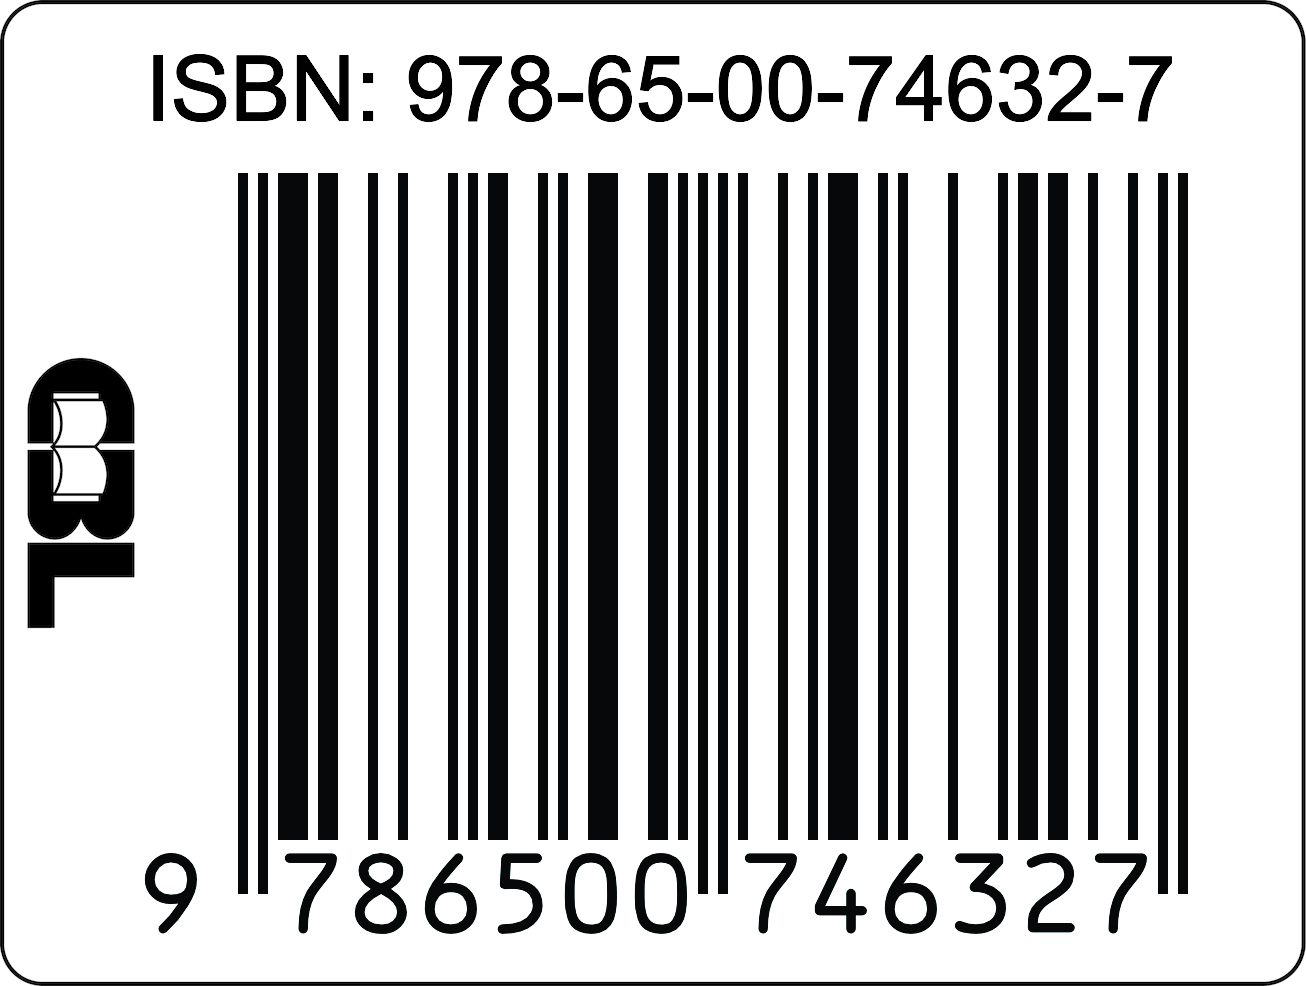
\includegraphics[scale=0.4,right]{imagens/isbn-978-65-00-74632-7-2ed}
    \end{figure}
    
    \restoregeometry
    
\end{titlingpage}


\end{document}